\documentclass[twoside]{book}

% Packages required by doxygen
\usepackage{calc}
\usepackage{doxygen}
\usepackage{graphicx}
\usepackage[utf8]{inputenc}
\usepackage{makeidx}
\usepackage{multicol}
\usepackage{multirow}
\usepackage{textcomp}
\usepackage[table]{xcolor}

% Font selection
\usepackage[T1]{fontenc}
\usepackage{mathptmx}
\usepackage[scaled=.90]{helvet}
\usepackage{courier}
\usepackage{amssymb}
\usepackage{sectsty}
\renewcommand{\familydefault}{\sfdefault}
\allsectionsfont{%
  \fontseries{bc}\selectfont%
  \color{darkgray}%
}
\renewcommand{\DoxyLabelFont}{%
  \fontseries{bc}\selectfont%
  \color{darkgray}%
}

% Page & text layout
\usepackage{geometry}
\geometry{%
  a4paper,%
  top=2.5cm,%
  bottom=2.5cm,%
  left=2.5cm,%
  right=2.5cm%
}
\tolerance=750
\hfuzz=15pt
\hbadness=750
\setlength{\emergencystretch}{15pt}
\setlength{\parindent}{0cm}
\setlength{\parskip}{0.2cm}
\makeatletter
\renewcommand{\paragraph}{%
  \@startsection{paragraph}{4}{0ex}{-1.0ex}{1.0ex}{%
    \normalfont\normalsize\bfseries\SS@parafont%
  }%
}
\renewcommand{\subparagraph}{%
  \@startsection{subparagraph}{5}{0ex}{-1.0ex}{1.0ex}{%
    \normalfont\normalsize\bfseries\SS@subparafont%
  }%
}
\makeatother

% Headers & footers
\usepackage{fancyhdr}
\pagestyle{fancyplain}
\fancyhead[LE]{\fancyplain{}{\bfseries\thepage}}
\fancyhead[CE]{\fancyplain{}{}}
\fancyhead[RE]{\fancyplain{}{\bfseries\leftmark}}
\fancyhead[LO]{\fancyplain{}{\bfseries\rightmark}}
\fancyhead[CO]{\fancyplain{}{}}
\fancyhead[RO]{\fancyplain{}{\bfseries\thepage}}
\fancyfoot[LE]{\fancyplain{}{}}
\fancyfoot[CE]{\fancyplain{}{}}
\fancyfoot[RE]{\fancyplain{}{\bfseries\scriptsize Generated on Fri Dec 11 2020 14\-:20\-:22 for Victre 2.\-0 Pipeline by Doxygen }}
\fancyfoot[LO]{\fancyplain{}{\bfseries\scriptsize Generated on Fri Dec 11 2020 14\-:20\-:22 for Victre 2.\-0 Pipeline by Doxygen }}
\fancyfoot[CO]{\fancyplain{}{}}
\fancyfoot[RO]{\fancyplain{}{}}
\renewcommand{\footrulewidth}{0.4pt}
\renewcommand{\chaptermark}[1]{%
  \markboth{#1}{}%
}
\renewcommand{\sectionmark}[1]{%
  \markright{\thesection\ #1}%
}

% Indices & bibliography
\usepackage{natbib}
\usepackage[titles]{tocloft}
\setcounter{tocdepth}{3}
\setcounter{secnumdepth}{5}
\makeindex

% Hyperlinks (required, but should be loaded last)
\usepackage{ifpdf}
\ifpdf
  \usepackage[pdftex,pagebackref=true]{hyperref}
\else
  \usepackage[ps2pdf,pagebackref=true]{hyperref}
\fi
\hypersetup{%
  colorlinks=true,%
  linkcolor=blue,%
  citecolor=blue,%
  unicode%
}

% Custom commands
\newcommand{\clearemptydoublepage}{%
  \newpage{\pagestyle{empty}\cleardoublepage}%
}


%===== C O N T E N T S =====

\begin{document}

% Titlepage & ToC
\hypersetup{pageanchor=false}
\pagenumbering{roman}
\begin{titlepage}
\vspace*{7cm}
\begin{center}%
{\Large Victre 2.0 Pipeline \\[1ex]\large 0.\-0.\-1 }\\
\vspace*{1cm}
{\large Generated by Doxygen 1.8.5}\\
\vspace*{0.5cm}
{\small Fri Dec 11 2020 14:20:22}\\
\end{center}
\end{titlepage}
\clearemptydoublepage
\tableofcontents
\clearemptydoublepage
\pagenumbering{arabic}
\hypersetup{pageanchor=true}

%--- Begin generated contents ---
\chapter{breast\-Mass}
\label{md_Victre_breastMass_README}
\hypertarget{md_Victre_breastMass_README}{}
Breast Mass Generation Software

{\bfseries Documentation and installation instructions are available here\-:} \href{https://breastMass.readthedocs.io}{\tt breast\-Mass.\-readthedocs.\-io}.

The project is in the public domain within the United States, and copyright and related rights in the work worldwide are waived through the C\-C0 1.\-0 Universal public domain dedication. See the C\-O\-P\-Y\-I\-N\-G.\-txt file in this repository to view the entire C\-C0 dedication.

All contributions to this project will be released under the C\-C0 dedication. By submitting a pull request, you are agreeing to comply with this waiver of copyright interest.

\subsection*{Disclaimer}

This software and documentation (the \char`\"{}\-Software\char`\"{}) were developed at the Food and Drug Administration (F\-D\-A) by employees of the Federal Government in the course of their official duties. Pursuant to Title 17, Section 105 of the United States Code, this work is not subject to copyright protection and is in the public domain. Permission is hereby granted, free of charge, to any person obtaining a copy of the Software, to deal in the Software without restriction, including without limitation the rights to use, copy, modify, merge, publish, distribute, sublicense, or sell copies of the Software or derivatives, and to permit persons to whom the Software is furnished to do so. F\-D\-A assumes no responsibility whatsoever for use by other parties of the Software, its source code, documentation or compiled executables, and makes no guarantees, expressed or implied, about its quality, reliability, or any other characteristic. Further, use of this code in no way implies endorsement by the F\-D\-A or confers any advantage in regulatory decisions. Although this software can be redistributed and/or modified freely, we ask that any derivative works bear some notice that they are derived from it, and any modified versions bear some notice that they have been modified. 
\chapter{Namespace Index}
\section{Namespace List}
Here is a list of all namespaces with brief descriptions\-:\begin{DoxyCompactList}
\item\contentsline{section}{\hyperlink{namespaceconf}{conf} }{\pageref{namespaceconf}}{}
\item\contentsline{section}{\hyperlink{namespaceget__average__lesion}{get\-\_\-average\-\_\-lesion} }{\pageref{namespaceget__average__lesion}}{}
\item\contentsline{section}{\hyperlink{namespacerun__pipeline}{run\-\_\-pipeline} }{\pageref{namespacerun__pipeline}}{}
\item\contentsline{section}{\hyperlink{namespacerun__pipeline__lesionsizes}{run\-\_\-pipeline\-\_\-lesionsizes} }{\pageref{namespacerun__pipeline__lesionsizes}}{}
\item\contentsline{section}{\hyperlink{namespacetest__pipeline}{test\-\_\-pipeline} }{\pageref{namespacetest__pipeline}}{}
\item\contentsline{section}{\hyperlink{namespacetest__spiculated}{test\-\_\-spiculated} }{\pageref{namespacetest__spiculated}}{}
\item\contentsline{section}{\hyperlink{namespaceVictre}{Victre} }{\pageref{namespaceVictre}}{}
\item\contentsline{section}{\hyperlink{namespaceVictre_1_1Constants}{Victre.\-Constants} }{\pageref{namespaceVictre_1_1Constants}}{}
\item\contentsline{section}{\hyperlink{namespaceVictre_1_1Exceptions}{Victre.\-Exceptions} }{\pageref{namespaceVictre_1_1Exceptions}}{}
\item\contentsline{section}{\hyperlink{namespaceVictre_1_1Pipeline}{Victre.\-Pipeline} \\*\subsubsection*{Documentation for the \hyperlink{namespaceVictre}{Victre} pipeline class.}}{\pageref{namespaceVictre_1_1Pipeline}}{}
\end{DoxyCompactList}

\chapter{Hierarchical Index}
\section{Class Hierarchy}
This inheritance list is sorted roughly, but not completely, alphabetically\-:\begin{DoxyCompactList}
\item Exception\begin{DoxyCompactList}
\item \contentsline{section}{Victre.\-Exceptions.\-Victre\-Error}{\pageref{classVictre_1_1Exceptions_1_1VictreError}}{}
\end{DoxyCompactList}
\item \contentsline{section}{perturb}{\pageref{structperturb}}{}
\item \contentsline{section}{Victre.\-Pipeline.\-Pipeline}{\pageref{classVictre_1_1Pipeline_1_1Pipeline}}{}
\end{DoxyCompactList}

\chapter{Class Index}
\section{Class List}
Here are the classes, structs, unions and interfaces with brief descriptions\-:\begin{DoxyCompactList}
\item\contentsline{section}{\hyperlink{structperturb}{perturb} }{\pageref{structperturb}}{}
\item\contentsline{section}{\hyperlink{classVictre_1_1Pipeline_1_1Pipeline}{Victre.\-Pipeline.\-Pipeline} }{\pageref{classVictre_1_1Pipeline_1_1Pipeline}}{}
\item\contentsline{section}{\hyperlink{classVictre_1_1Exceptions_1_1VictreError}{Victre.\-Exceptions.\-Victre\-Error} }{\pageref{classVictre_1_1Exceptions_1_1VictreError}}{}
\end{DoxyCompactList}

\chapter{File Index}
\section{File List}
Here is a list of all files with brief descriptions\-:\begin{DoxyCompactList}
\item\contentsline{section}{\hyperlink{get__average__lesion_8py}{get\-\_\-average\-\_\-lesion.\-py} }{\pageref{get__average__lesion_8py}}{}
\item\contentsline{section}{\hyperlink{run__pipeline_8py}{run\-\_\-pipeline.\-py} }{\pageref{run__pipeline_8py}}{}
\item\contentsline{section}{\hyperlink{run__pipeline__lesionsizes_8py}{run\-\_\-pipeline\-\_\-lesionsizes.\-py} }{\pageref{run__pipeline__lesionsizes_8py}}{}
\item\contentsline{section}{\hyperlink{test__pipeline_8py}{test\-\_\-pipeline.\-py} }{\pageref{test__pipeline_8py}}{}
\item\contentsline{section}{\hyperlink{test__spiculated_8py}{test\-\_\-spiculated.\-py} }{\pageref{test__spiculated_8py}}{}
\item\contentsline{section}{Victre/\hyperlink{____init_____8py}{\-\_\-\-\_\-init\-\_\-\-\_\-.\-py} }{\pageref{____init_____8py}}{}
\item\contentsline{section}{Victre/\hyperlink{Constants_8py}{Constants.\-py} }{\pageref{Constants_8py}}{}
\item\contentsline{section}{Victre/\hyperlink{Exceptions_8py}{Exceptions.\-py} }{\pageref{Exceptions_8py}}{}
\item\contentsline{section}{Victre/\hyperlink{Pipeline_8py}{Pipeline.\-py} }{\pageref{Pipeline_8py}}{}
\item\contentsline{section}{Victre/breast\-Mass/\hyperlink{breastMass_8cxx}{breast\-Mass.\-cxx} \\*Breast\-Mass main source file }{\pageref{breastMass_8cxx}}{}
\item\contentsline{section}{Victre/breast\-Mass/\hyperlink{breastMass_8hxx}{breast\-Mass.\-hxx} \\*Breast\-Mass header file }{\pageref{breastMass_8hxx}}{}
\item\contentsline{section}{Victre/breast\-Mass/\-C\-Make\-Files/2.\-8.\-12.\-2/\-Compiler\-Id\-C/\hyperlink{CMakeCCompilerId_8c}{C\-Make\-C\-Compiler\-Id.\-c} }{\pageref{CMakeCCompilerId_8c}}{}
\item\contentsline{section}{Victre/breast\-Mass/\-C\-Make\-Files/2.\-8.\-12.\-2/\-Compiler\-Id\-C\-X\-X/\hyperlink{CMakeCXXCompilerId_8cpp}{C\-Make\-C\-X\-X\-Compiler\-Id.\-cpp} }{\pageref{CMakeCXXCompilerId_8cpp}}{}
\item\contentsline{section}{Victre/breast\-Mass/doc/\hyperlink{conf_8py}{conf.\-py} }{\pageref{conf_8py}}{}
\item\contentsline{section}{Victre/reconstruction/\hyperlink{FBP__DBTrecon_8h}{F\-B\-P\-\_\-\-D\-B\-Trecon.\-h} }{\pageref{FBP__DBTrecon_8h}}{}
\item\contentsline{section}{Victre/reconstruction/\hyperlink{FBP__DBTrecon__dense__SA_8c}{F\-B\-P\-\_\-\-D\-B\-Trecon\-\_\-dense\-\_\-\-S\-A.\-c} }{\pageref{FBP__DBTrecon__dense__SA_8c}}{}
\item\contentsline{section}{Victre/reconstruction/\hyperlink{FBP__DBTrecon__dense__SP_8c}{F\-B\-P\-\_\-\-D\-B\-Trecon\-\_\-dense\-\_\-\-S\-P.\-c} }{\pageref{FBP__DBTrecon__dense__SP_8c}}{}
\item\contentsline{section}{Victre/reconstruction/\hyperlink{FBP__DBTrecon__fatty__SA_8c}{F\-B\-P\-\_\-\-D\-B\-Trecon\-\_\-fatty\-\_\-\-S\-A.\-c} }{\pageref{FBP__DBTrecon__fatty__SA_8c}}{}
\item\contentsline{section}{Victre/reconstruction/\hyperlink{FBP__DBTrecon__fatty__SP_8c}{F\-B\-P\-\_\-\-D\-B\-Trecon\-\_\-fatty\-\_\-\-S\-P.\-c} }{\pageref{FBP__DBTrecon__fatty__SP_8c}}{}
\item\contentsline{section}{Victre/reconstruction/\hyperlink{FBP__DBTrecon__hetero__SA_8c}{F\-B\-P\-\_\-\-D\-B\-Trecon\-\_\-hetero\-\_\-\-S\-A.\-c} }{\pageref{FBP__DBTrecon__hetero__SA_8c}}{}
\item\contentsline{section}{Victre/reconstruction/\hyperlink{FBP__DBTrecon__hetero__SP_8c}{F\-B\-P\-\_\-\-D\-B\-Trecon\-\_\-hetero\-\_\-\-S\-P.\-c} }{\pageref{FBP__DBTrecon__hetero__SP_8c}}{}
\item\contentsline{section}{Victre/reconstruction/\hyperlink{FBP__DBTrecon__scattered__SA_8c}{F\-B\-P\-\_\-\-D\-B\-Trecon\-\_\-scattered\-\_\-\-S\-A.\-c} }{\pageref{FBP__DBTrecon__scattered__SA_8c}}{}
\item\contentsline{section}{Victre/reconstruction/\hyperlink{FBP__DBTrecon__scattered__SP_8c}{F\-B\-P\-\_\-\-D\-B\-Trecon\-\_\-scattered\-\_\-\-S\-P.\-c} }{\pageref{FBP__DBTrecon__scattered__SP_8c}}{}
\item\contentsline{section}{Victre/reconstruction/\-Aunnasha\-\_\-code\-\_\-read\-\_\-inputfile/\hyperlink{Aunnasha__code__read__inputfile_2FBP__DBTrecon_8c}{F\-B\-P\-\_\-\-D\-B\-Trecon.\-c} }{\pageref{Aunnasha__code__read__inputfile_2FBP__DBTrecon_8c}}{}
\item\contentsline{section}{Victre/reconstruction/\-Aunnasha\-\_\-code\-\_\-read\-\_\-inputfile/\hyperlink{Aunnasha__code__read__inputfile_2FBP__DBTrecon_8h}{F\-B\-P\-\_\-\-D\-B\-Trecon.\-h} }{\pageref{Aunnasha__code__read__inputfile_2FBP__DBTrecon_8h}}{}
\item\contentsline{section}{Victre/reconstruction/\-Aunnasha\-\_\-code\-\_\-read\-\_\-inputfile/\hyperlink{FBP__DBTrecon__dense__VICTRE_8c}{F\-B\-P\-\_\-\-D\-B\-Trecon\-\_\-dense\-\_\-\-V\-I\-C\-T\-R\-E.\-c} }{\pageref{FBP__DBTrecon__dense__VICTRE_8c}}{}
\item\contentsline{section}{Victre/reconstruction/cbct\-\_\-ccode/\hyperlink{coneBeam_8c}{cone\-Beam.\-c} }{\pageref{coneBeam_8c}}{}
\item\contentsline{section}{Victre/reconstruction/cbct\-\_\-ccode/\hyperlink{coneBeam_8h}{cone\-Beam.\-h} }{\pageref{coneBeam_8h}}{}
\item\contentsline{section}{Victre/reconstruction/cbct\-\_\-ccode/\hyperlink{coneBeam__VictreBreast__JUl25_8c}{cone\-Beam\-\_\-\-Victre\-Breast\-\_\-\-J\-Ul25.\-c} }{\pageref{coneBeam__VictreBreast__JUl25_8c}}{}
\item\contentsline{section}{Victre/reconstruction/cbct\-\_\-ccode/\hyperlink{coneBeam__VictreJul12__breast_8c}{cone\-Beam\-\_\-\-Victre\-Jul12\-\_\-breast.\-c} }{\pageref{coneBeam__VictreJul12__breast_8c}}{}
\item\contentsline{section}{Victre/reconstruction/cbct\-\_\-ccode/\hyperlink{coneBeam__VictreJul12__calibration_8c}{cone\-Beam\-\_\-\-Victre\-Jul12\-\_\-calibration.\-c} }{\pageref{coneBeam__VictreJul12__calibration_8c}}{}
\item\contentsline{section}{Victre/reconstruction/cbct\-\_\-ccode/\hyperlink{coneBeam__VictreJul6_8c}{cone\-Beam\-\_\-\-Victre\-Jul6.\-c} }{\pageref{coneBeam__VictreJul6_8c}}{}
\item\contentsline{section}{Victre/reconstruction/cbct\-\_\-ccode/\hyperlink{coneBeamDBT_8c}{cone\-Beam\-D\-B\-T.\-c} }{\pageref{coneBeamDBT_8c}}{}
\item\contentsline{section}{Victre/reconstruction/cbct\-\_\-ccode/\hyperlink{coneBeamDBTJun16_01_07copy_08_8c}{cone\-Beam\-D\-B\-T\-Jun16 (copy).\-c} }{\pageref{coneBeamDBTJun16_01_07copy_08_8c}}{}
\item\contentsline{section}{Victre/reconstruction/cbct\-\_\-ccode/\hyperlink{coneBeamDBTJun19_8c}{cone\-Beam\-D\-B\-T\-Jun19.\-c} }{\pageref{coneBeamDBTJun19_8c}}{}
\item\contentsline{section}{Victre/reconstruction/cbct\-\_\-ccode/\hyperlink{coneBeamDBTJun23_8c}{cone\-Beam\-D\-B\-T\-Jun23.\-c} }{\pageref{coneBeamDBTJun23_8c}}{}
\item\contentsline{section}{Victre/reconstruction/cbct\-\_\-ccode/\hyperlink{coneBeamDBTJun28rpz_8c}{cone\-Beam\-D\-B\-T\-Jun28rpz.\-c} }{\pageref{coneBeamDBTJun28rpz_8c}}{}
\item\contentsline{section}{Victre/reconstruction/cbct\-\_\-ccode/\hyperlink{coneBeamJun12_01_07copy_08_8c}{cone\-Beam\-Jun12 (copy).\-c} }{\pageref{coneBeamJun12_01_07copy_08_8c}}{}
\item\contentsline{section}{Victre/reconstruction/cbct\-\_\-ccode/\hyperlink{coneBeamJun12_8c}{cone\-Beam\-Jun12.\-c} }{\pageref{coneBeamJun12_8c}}{}
\item\contentsline{section}{Victre/reconstruction/cbct\-\_\-ccode/\hyperlink{coneBeamVictreJun30_8c}{cone\-Beam\-Victre\-Jun30.\-c} }{\pageref{coneBeamVictreJun30_8c}}{}
\item\contentsline{section}{Victre/reconstruction/cbct\-\_\-ccode/\hyperlink{cbct__ccode_2FBP__DBTrecon_8c}{F\-B\-P\-\_\-\-D\-B\-Trecon.\-c} }{\pageref{cbct__ccode_2FBP__DBTrecon_8c}}{}
\item\contentsline{section}{Victre/reconstruction/cbct\-\_\-ccode/\hyperlink{olderversiondata_8c}{olderversiondata.\-c} }{\pageref{olderversiondata_8c}}{}
\end{DoxyCompactList}

\chapter{Namespace Documentation}
\hypertarget{namespaceconf}{\section{conf Namespace Reference}
\label{namespaceconf}\index{conf@{conf}}
}
\subsection*{Variables}
\begin{DoxyCompactItemize}
\item 
list \hyperlink{namespaceconf_ae475e080536acb271a0a0efe56c3ba42}{extensions}
\item 
list \hyperlink{namespaceconf_ae850ae634911b713e036b43894fdd525}{templates\-\_\-path} = \mbox{[}'\-\_\-templates'\mbox{]}
\item 
string \hyperlink{namespaceconf_a10af2a769eb3bd3322e874f677e435b1}{source\-\_\-suffix} = '.rst'
\item 
string \hyperlink{namespaceconf_a6fcd7e5236f355b1e1a55f9d95988810}{master\-\_\-doc} = 'index'
\item 
string \hyperlink{namespaceconf_a45653c983098153b78e33600e39230eb}{project} = u'breast\-Mass'
\item 
string \hyperlink{namespaceconf_a33fa97cf51dcb25970fbf53f10159589}{copyright} = u'2018, Christian G. Graff'
\item 
string \hyperlink{namespaceconf_a637c239d256432248aa8d9f3ab0b8c52}{author} = u'Christian G. Graff'
\item 
string \hyperlink{namespaceconf_ade15c5b54093b64d7c428ec19ca5b1cb}{version} = u'1.\-0'
\item 
string \hyperlink{namespaceconf_a325dc746d8bf05c54d26351c35a21d90}{release} = u'1.\-0'
\item 
\hyperlink{namespaceconf_ad76a2e6d7bfa880ebb4042c08e8b4e12}{language} = None
\item 
list \hyperlink{namespaceconf_a7ad48fb6f3e9b129c02346ea0d3527c1}{exclude\-\_\-patterns} = \mbox{[}'\-\_\-build', 'Thumbs.\-db', '.D\-S\-\_\-\-Store'\mbox{]}
\item 
string \hyperlink{namespaceconf_a641130e096b26cba8a5d63ed38684de7}{pygments\-\_\-style} = 'sphinx'
\item 
\hyperlink{namespaceconf_a997cbdffcb2f28023aba4c37bbf469b5}{todo\-\_\-include\-\_\-todos} = False
\item 
string \hyperlink{namespaceconf_a6c3bfcc1a44546c1c75ce20f55bd0fd6}{html\-\_\-theme} = 'alabaster'
\item 
dictionary \hyperlink{namespaceconf_aeaafa42217d24810edc9b116b88a4585}{html\-\_\-theme\-\_\-options}
\item 
\hyperlink{namespaceconf_aef058dc18c5e6a45d2cebad007a465c7}{html\-\_\-show\-\_\-copyright} = False
\item 
list \hyperlink{namespaceconf_af4fb5d8851ccaade135c2668dd3ced41}{html\-\_\-static\-\_\-path} = \mbox{[}'\-\_\-static'\mbox{]}
\item 
dictionary \hyperlink{namespaceconf_a3f3b198d720ed6fab15e95fa2479adb6}{html\-\_\-sidebars}
\item 
string \hyperlink{namespaceconf_aab7fddb2766ce3c430d8246fbfdbc7b1}{htmlhelp\-\_\-basename} = 'breast\-Massdoc'
\item 
dictionary \hyperlink{namespaceconf_a33619d385ad23765ac6ebb58bf82d43d}{latex\-\_\-elements}
\item 
list \hyperlink{namespaceconf_a7812f49970f3de0d15dd7b9b9a10e3a1}{latex\-\_\-documents}
\item 
list \hyperlink{namespaceconf_a85efc5fee48a26fa2d651f6eeb38fc2b}{man\-\_\-pages}
\item 
list \hyperlink{namespaceconf_a54b0faed214ac92017d5689efbb10672}{texinfo\-\_\-documents}
\item 
dictionary \hyperlink{namespaceconf_a8375f4f963de3ac8026eaa9beced9564}{intersphinx\-\_\-mapping} = \{'https\-://docs.\-python.\-org/'\-: None\}
\end{DoxyCompactItemize}


\subsection{Variable Documentation}
\hypertarget{namespaceconf_a637c239d256432248aa8d9f3ab0b8c52}{\index{conf@{conf}!author@{author}}
\index{author@{author}!conf@{conf}}
\subsubsection[{author}]{\setlength{\rightskip}{0pt plus 5cm}string conf.\-author = u'Christian G. Graff'}}\label{namespaceconf_a637c239d256432248aa8d9f3ab0b8c52}
\hypertarget{namespaceconf_a33fa97cf51dcb25970fbf53f10159589}{\index{conf@{conf}!copyright@{copyright}}
\index{copyright@{copyright}!conf@{conf}}
\subsubsection[{copyright}]{\setlength{\rightskip}{0pt plus 5cm}string conf.\-copyright = u'2018, Christian G. Graff'}}\label{namespaceconf_a33fa97cf51dcb25970fbf53f10159589}
\hypertarget{namespaceconf_a7ad48fb6f3e9b129c02346ea0d3527c1}{\index{conf@{conf}!exclude\-\_\-patterns@{exclude\-\_\-patterns}}
\index{exclude\-\_\-patterns@{exclude\-\_\-patterns}!conf@{conf}}
\subsubsection[{exclude\-\_\-patterns}]{\setlength{\rightskip}{0pt plus 5cm}list conf.\-exclude\-\_\-patterns = \mbox{[}'\-\_\-build', 'Thumbs.\-db', '.D\-S\-\_\-\-Store'\mbox{]}}}\label{namespaceconf_a7ad48fb6f3e9b129c02346ea0d3527c1}
\hypertarget{namespaceconf_ae475e080536acb271a0a0efe56c3ba42}{\index{conf@{conf}!extensions@{extensions}}
\index{extensions@{extensions}!conf@{conf}}
\subsubsection[{extensions}]{\setlength{\rightskip}{0pt plus 5cm}list conf.\-extensions}}\label{namespaceconf_ae475e080536acb271a0a0efe56c3ba42}
{\bfseries Initial value\-:}
\begin{DoxyCode}
1 = [\textcolor{stringliteral}{'sphinx.ext.intersphinx'},
2     \textcolor{stringliteral}{'sphinx.ext.mathjax'},
3     \textcolor{stringliteral}{'sphinx.ext.githubpages'}]
\end{DoxyCode}
\hypertarget{namespaceconf_aef058dc18c5e6a45d2cebad007a465c7}{\index{conf@{conf}!html\-\_\-show\-\_\-copyright@{html\-\_\-show\-\_\-copyright}}
\index{html\-\_\-show\-\_\-copyright@{html\-\_\-show\-\_\-copyright}!conf@{conf}}
\subsubsection[{html\-\_\-show\-\_\-copyright}]{\setlength{\rightskip}{0pt plus 5cm}conf.\-html\-\_\-show\-\_\-copyright = False}}\label{namespaceconf_aef058dc18c5e6a45d2cebad007a465c7}
\hypertarget{namespaceconf_a3f3b198d720ed6fab15e95fa2479adb6}{\index{conf@{conf}!html\-\_\-sidebars@{html\-\_\-sidebars}}
\index{html\-\_\-sidebars@{html\-\_\-sidebars}!conf@{conf}}
\subsubsection[{html\-\_\-sidebars}]{\setlength{\rightskip}{0pt plus 5cm}dictionary conf.\-html\-\_\-sidebars}}\label{namespaceconf_a3f3b198d720ed6fab15e95fa2479adb6}
{\bfseries Initial value\-:}
\begin{DoxyCode}
1 = \{
2     \textcolor{stringliteral}{'**'}: [
3         \textcolor{stringliteral}{'about.html'},
4         \textcolor{stringliteral}{'globaltoc.html'},
5         \textcolor{stringliteral}{'relations.html'},  \textcolor{comment}{# needs 'show\_related': True theme option to display}
6         \textcolor{stringliteral}{'searchbox.html'},
7     ]
8 \}
\end{DoxyCode}
\hypertarget{namespaceconf_af4fb5d8851ccaade135c2668dd3ced41}{\index{conf@{conf}!html\-\_\-static\-\_\-path@{html\-\_\-static\-\_\-path}}
\index{html\-\_\-static\-\_\-path@{html\-\_\-static\-\_\-path}!conf@{conf}}
\subsubsection[{html\-\_\-static\-\_\-path}]{\setlength{\rightskip}{0pt plus 5cm}list conf.\-html\-\_\-static\-\_\-path = \mbox{[}'\-\_\-static'\mbox{]}}}\label{namespaceconf_af4fb5d8851ccaade135c2668dd3ced41}
\hypertarget{namespaceconf_a6c3bfcc1a44546c1c75ce20f55bd0fd6}{\index{conf@{conf}!html\-\_\-theme@{html\-\_\-theme}}
\index{html\-\_\-theme@{html\-\_\-theme}!conf@{conf}}
\subsubsection[{html\-\_\-theme}]{\setlength{\rightskip}{0pt plus 5cm}string conf.\-html\-\_\-theme = 'alabaster'}}\label{namespaceconf_a6c3bfcc1a44546c1c75ce20f55bd0fd6}
\hypertarget{namespaceconf_aeaafa42217d24810edc9b116b88a4585}{\index{conf@{conf}!html\-\_\-theme\-\_\-options@{html\-\_\-theme\-\_\-options}}
\index{html\-\_\-theme\-\_\-options@{html\-\_\-theme\-\_\-options}!conf@{conf}}
\subsubsection[{html\-\_\-theme\-\_\-options}]{\setlength{\rightskip}{0pt plus 5cm}dictionary conf.\-html\-\_\-theme\-\_\-options}}\label{namespaceconf_aeaafa42217d24810edc9b116b88a4585}
{\bfseries Initial value\-:}
\begin{DoxyCode}
1 = \{
2     \textcolor{stringliteral}{'logo'}: \textcolor{stringliteral}{'massLogo.png'},
3     \textcolor{stringliteral}{'logo\_name'}: \textcolor{stringliteral}{'true'},
4     \textcolor{stringliteral}{'description'}: \textcolor{stringliteral}{'breast mass generation'},
5     \textcolor{stringliteral}{'font\_family'}: \textcolor{stringliteral}{'Helvetica'},
6     \textcolor{stringliteral}{'head\_font\_family'}: \textcolor{stringliteral}{'Helvetica'},
7     \textcolor{stringliteral}{'font\_size'}: \textcolor{stringliteral}{'12pt'},
8     \textcolor{stringliteral}{'fixed\_sidebar'}: \textcolor{stringliteral}{'true'},
9     \textcolor{stringliteral}{'page\_width'}: \textcolor{stringliteral}{'1200px'},
10     \textcolor{stringliteral}{'sidebar\_width'}: \textcolor{stringliteral}{'250px'},
11     \textcolor{stringliteral}{'github\_user'}: \textcolor{stringliteral}{'DIDSR'},
12     \textcolor{stringliteral}{'github\_repo'}: \textcolor{stringliteral}{'breastMass'},
13     \textcolor{stringliteral}{'github\_button'}: \textcolor{stringliteral}{'true'}
14 \}
\end{DoxyCode}
\hypertarget{namespaceconf_aab7fddb2766ce3c430d8246fbfdbc7b1}{\index{conf@{conf}!htmlhelp\-\_\-basename@{htmlhelp\-\_\-basename}}
\index{htmlhelp\-\_\-basename@{htmlhelp\-\_\-basename}!conf@{conf}}
\subsubsection[{htmlhelp\-\_\-basename}]{\setlength{\rightskip}{0pt plus 5cm}string conf.\-htmlhelp\-\_\-basename = 'breast\-Massdoc'}}\label{namespaceconf_aab7fddb2766ce3c430d8246fbfdbc7b1}
\hypertarget{namespaceconf_a8375f4f963de3ac8026eaa9beced9564}{\index{conf@{conf}!intersphinx\-\_\-mapping@{intersphinx\-\_\-mapping}}
\index{intersphinx\-\_\-mapping@{intersphinx\-\_\-mapping}!conf@{conf}}
\subsubsection[{intersphinx\-\_\-mapping}]{\setlength{\rightskip}{0pt plus 5cm}dictionary conf.\-intersphinx\-\_\-mapping = \{'https\-://docs.\-python.\-org/'\-: None\}}}\label{namespaceconf_a8375f4f963de3ac8026eaa9beced9564}
\hypertarget{namespaceconf_ad76a2e6d7bfa880ebb4042c08e8b4e12}{\index{conf@{conf}!language@{language}}
\index{language@{language}!conf@{conf}}
\subsubsection[{language}]{\setlength{\rightskip}{0pt plus 5cm}conf.\-language = None}}\label{namespaceconf_ad76a2e6d7bfa880ebb4042c08e8b4e12}
\hypertarget{namespaceconf_a7812f49970f3de0d15dd7b9b9a10e3a1}{\index{conf@{conf}!latex\-\_\-documents@{latex\-\_\-documents}}
\index{latex\-\_\-documents@{latex\-\_\-documents}!conf@{conf}}
\subsubsection[{latex\-\_\-documents}]{\setlength{\rightskip}{0pt plus 5cm}list conf.\-latex\-\_\-documents}}\label{namespaceconf_a7812f49970f3de0d15dd7b9b9a10e3a1}
{\bfseries Initial value\-:}
\begin{DoxyCode}
1 = [
2     (master\_doc, \textcolor{stringliteral}{'breastMass.tex'}, \textcolor{stringliteral}{u'breastMass Documentation'},
3      \textcolor{stringliteral}{u'Christian G. Graff'}, \textcolor{stringliteral}{'manual'}),
4 ]
\end{DoxyCode}
\hypertarget{namespaceconf_a33619d385ad23765ac6ebb58bf82d43d}{\index{conf@{conf}!latex\-\_\-elements@{latex\-\_\-elements}}
\index{latex\-\_\-elements@{latex\-\_\-elements}!conf@{conf}}
\subsubsection[{latex\-\_\-elements}]{\setlength{\rightskip}{0pt plus 5cm}dictionary conf.\-latex\-\_\-elements}}\label{namespaceconf_a33619d385ad23765ac6ebb58bf82d43d}
{\bfseries Initial value\-:}
\begin{DoxyCode}
1 = \{
2     \textcolor{comment}{# The paper size ('letterpaper' or 'a4paper').}
3     \textcolor{comment}{#}
4     \textcolor{comment}{# 'papersize': 'letterpaper',}
5 
6     \textcolor{comment}{# The font size ('10pt', '11pt' or '12pt').}
7     \textcolor{comment}{#}
8     \textcolor{comment}{# 'pointsize': '10pt',}
9 
10     \textcolor{comment}{# Additional stuff for the LaTeX preamble.}
11     \textcolor{comment}{#}
12     \textcolor{comment}{# 'preamble': '',}
13 
14     \textcolor{comment}{# Latex figure (float) alignment}
15     \textcolor{comment}{#}
16     \textcolor{comment}{# 'figure\_align': 'htbp',}
17     \textcolor{stringliteral}{'extraclassoptions'}: \textcolor{stringliteral}{'openany,oneside'}    
18 \}
\end{DoxyCode}
\hypertarget{namespaceconf_a85efc5fee48a26fa2d651f6eeb38fc2b}{\index{conf@{conf}!man\-\_\-pages@{man\-\_\-pages}}
\index{man\-\_\-pages@{man\-\_\-pages}!conf@{conf}}
\subsubsection[{man\-\_\-pages}]{\setlength{\rightskip}{0pt plus 5cm}list conf.\-man\-\_\-pages}}\label{namespaceconf_a85efc5fee48a26fa2d651f6eeb38fc2b}
{\bfseries Initial value\-:}
\begin{DoxyCode}
1 = [
2     (master\_doc, \textcolor{stringliteral}{'breastmass'}, \textcolor{stringliteral}{u'breastMass Documentation'},
3      [author], 1)
4 ]
\end{DoxyCode}
\hypertarget{namespaceconf_a6fcd7e5236f355b1e1a55f9d95988810}{\index{conf@{conf}!master\-\_\-doc@{master\-\_\-doc}}
\index{master\-\_\-doc@{master\-\_\-doc}!conf@{conf}}
\subsubsection[{master\-\_\-doc}]{\setlength{\rightskip}{0pt plus 5cm}string conf.\-master\-\_\-doc = 'index'}}\label{namespaceconf_a6fcd7e5236f355b1e1a55f9d95988810}
\hypertarget{namespaceconf_a45653c983098153b78e33600e39230eb}{\index{conf@{conf}!project@{project}}
\index{project@{project}!conf@{conf}}
\subsubsection[{project}]{\setlength{\rightskip}{0pt plus 5cm}string conf.\-project = u'breast\-Mass'}}\label{namespaceconf_a45653c983098153b78e33600e39230eb}
\hypertarget{namespaceconf_a641130e096b26cba8a5d63ed38684de7}{\index{conf@{conf}!pygments\-\_\-style@{pygments\-\_\-style}}
\index{pygments\-\_\-style@{pygments\-\_\-style}!conf@{conf}}
\subsubsection[{pygments\-\_\-style}]{\setlength{\rightskip}{0pt plus 5cm}string conf.\-pygments\-\_\-style = 'sphinx'}}\label{namespaceconf_a641130e096b26cba8a5d63ed38684de7}
\hypertarget{namespaceconf_a325dc746d8bf05c54d26351c35a21d90}{\index{conf@{conf}!release@{release}}
\index{release@{release}!conf@{conf}}
\subsubsection[{release}]{\setlength{\rightskip}{0pt plus 5cm}string conf.\-release = u'1.\-0'}}\label{namespaceconf_a325dc746d8bf05c54d26351c35a21d90}
\hypertarget{namespaceconf_a10af2a769eb3bd3322e874f677e435b1}{\index{conf@{conf}!source\-\_\-suffix@{source\-\_\-suffix}}
\index{source\-\_\-suffix@{source\-\_\-suffix}!conf@{conf}}
\subsubsection[{source\-\_\-suffix}]{\setlength{\rightskip}{0pt plus 5cm}string conf.\-source\-\_\-suffix = '.rst'}}\label{namespaceconf_a10af2a769eb3bd3322e874f677e435b1}
\hypertarget{namespaceconf_ae850ae634911b713e036b43894fdd525}{\index{conf@{conf}!templates\-\_\-path@{templates\-\_\-path}}
\index{templates\-\_\-path@{templates\-\_\-path}!conf@{conf}}
\subsubsection[{templates\-\_\-path}]{\setlength{\rightskip}{0pt plus 5cm}list conf.\-templates\-\_\-path = \mbox{[}'\-\_\-templates'\mbox{]}}}\label{namespaceconf_ae850ae634911b713e036b43894fdd525}
\hypertarget{namespaceconf_a54b0faed214ac92017d5689efbb10672}{\index{conf@{conf}!texinfo\-\_\-documents@{texinfo\-\_\-documents}}
\index{texinfo\-\_\-documents@{texinfo\-\_\-documents}!conf@{conf}}
\subsubsection[{texinfo\-\_\-documents}]{\setlength{\rightskip}{0pt plus 5cm}list conf.\-texinfo\-\_\-documents}}\label{namespaceconf_a54b0faed214ac92017d5689efbb10672}
{\bfseries Initial value\-:}
\begin{DoxyCode}
1 = [
2     (master\_doc, \textcolor{stringliteral}{'breastMass'}, \textcolor{stringliteral}{u'breastMass Documentation'},
3      author, \textcolor{stringliteral}{'breastMass'}, \textcolor{stringliteral}{'breast mass generation'},
4      \textcolor{stringliteral}{'Miscellaneous'}),
5 ]
\end{DoxyCode}
\hypertarget{namespaceconf_a997cbdffcb2f28023aba4c37bbf469b5}{\index{conf@{conf}!todo\-\_\-include\-\_\-todos@{todo\-\_\-include\-\_\-todos}}
\index{todo\-\_\-include\-\_\-todos@{todo\-\_\-include\-\_\-todos}!conf@{conf}}
\subsubsection[{todo\-\_\-include\-\_\-todos}]{\setlength{\rightskip}{0pt plus 5cm}conf.\-todo\-\_\-include\-\_\-todos = False}}\label{namespaceconf_a997cbdffcb2f28023aba4c37bbf469b5}
\hypertarget{namespaceconf_ade15c5b54093b64d7c428ec19ca5b1cb}{\index{conf@{conf}!version@{version}}
\index{version@{version}!conf@{conf}}
\subsubsection[{version}]{\setlength{\rightskip}{0pt plus 5cm}string conf.\-version = u'1.\-0'}}\label{namespaceconf_ade15c5b54093b64d7c428ec19ca5b1cb}

\hypertarget{namespaceget__average__lesion}{\section{get\-\_\-average\-\_\-lesion Namespace Reference}
\label{namespaceget__average__lesion}\index{get\-\_\-average\-\_\-lesion@{get\-\_\-average\-\_\-lesion}}
}
\subsection*{Functions}
\begin{DoxyCompactItemize}
\item 
def \hyperlink{namespaceget__average__lesion_a6fa4030a8ff4bd77b404c5c5fe1dcba0}{get\-\_\-folder\-\_\-contents}
\end{DoxyCompactItemize}
\subsection*{Variables}
\begin{DoxyCompactItemize}
\item 
dictionary \hyperlink{namespaceget__average__lesion_a04e4f7fdef2b31493b5aab71ddf47d7f}{lesion\-\_\-str}
\item 
tuple \hyperlink{namespaceget__average__lesion_a18dd42d421835ddf04df21748b1fbd97}{phantoms} = \hyperlink{namespaceget__average__lesion_a6fa4030a8ff4bd77b404c5c5fe1dcba0}{get\-\_\-folder\-\_\-contents}(\char`\"{}results\char`\"{})
\item 
dictionary \hyperlink{namespaceget__average__lesion_a1fd4bf63fb19d5891e9e0d3390074201}{mean}
\item 
int \hyperlink{namespaceget__average__lesion_aa8eb6c12f2c638c3c97b5cbb4f7aa6b0}{num\-\_\-cases} = 3
\item 
tuple \hyperlink{namespaceget__average__lesion_af4a292c67ad6c19a4faf0f86f5aa0f45}{rois} = h5py.\-File(ph + \char`\"{}/R\-O\-Is.\-h5\char`\"{}, \char`\"{}r\char`\"{})
\end{DoxyCompactItemize}


\subsection{Function Documentation}
\hypertarget{namespaceget__average__lesion_a6fa4030a8ff4bd77b404c5c5fe1dcba0}{\index{get\-\_\-average\-\_\-lesion@{get\-\_\-average\-\_\-lesion}!get\-\_\-folder\-\_\-contents@{get\-\_\-folder\-\_\-contents}}
\index{get\-\_\-folder\-\_\-contents@{get\-\_\-folder\-\_\-contents}!get_average_lesion@{get\-\_\-average\-\_\-lesion}}
\subsubsection[{get\-\_\-folder\-\_\-contents}]{\setlength{\rightskip}{0pt plus 5cm}def get\-\_\-average\-\_\-lesion.\-get\-\_\-folder\-\_\-contents (
\begin{DoxyParamCaption}
\item[{}]{folder}
\end{DoxyParamCaption}
)}}\label{namespaceget__average__lesion_a6fa4030a8ff4bd77b404c5c5fe1dcba0}


\subsection{Variable Documentation}
\hypertarget{namespaceget__average__lesion_a04e4f7fdef2b31493b5aab71ddf47d7f}{\index{get\-\_\-average\-\_\-lesion@{get\-\_\-average\-\_\-lesion}!lesion\-\_\-str@{lesion\-\_\-str}}
\index{lesion\-\_\-str@{lesion\-\_\-str}!get_average_lesion@{get\-\_\-average\-\_\-lesion}}
\subsubsection[{lesion\-\_\-str}]{\setlength{\rightskip}{0pt plus 5cm}dictionary get\-\_\-average\-\_\-lesion.\-lesion\-\_\-str}}\label{namespaceget__average__lesion_a04e4f7fdef2b31493b5aab71ddf47d7f}
{\bfseries Initial value\-:}
\begin{DoxyCode}
1 = \{Constants.VICTRE\_CLUSTERCALC: \textcolor{stringliteral}{"clustercalc"},
2               Constants.VICTRE\_SPICULATED: \textcolor{stringliteral}{"spiculated"}\}
\end{DoxyCode}
\hypertarget{namespaceget__average__lesion_a1fd4bf63fb19d5891e9e0d3390074201}{\index{get\-\_\-average\-\_\-lesion@{get\-\_\-average\-\_\-lesion}!mean@{mean}}
\index{mean@{mean}!get_average_lesion@{get\-\_\-average\-\_\-lesion}}
\subsubsection[{mean}]{\setlength{\rightskip}{0pt plus 5cm}dictionary get\-\_\-average\-\_\-lesion.\-mean}}\label{namespaceget__average__lesion_a1fd4bf63fb19d5891e9e0d3390074201}
{\bfseries Initial value\-:}
\begin{DoxyCode}
1 = \{\textcolor{stringliteral}{"dbt"}: \{Constants.VICTRE\_CLUSTERCALC: np.zeros((5, 65, 65)),
2                 Constants.VICTRE\_SPICULATED: np.zeros((9, 109, 109))\},
3         \textcolor{stringliteral}{"dm"}: \{Constants.VICTRE\_CLUSTERCALC: np.zeros((65, 65)),
4                Constants.VICTRE\_SPICULATED: np.zeros((109, 109))\}
5         \}
\end{DoxyCode}
\hypertarget{namespaceget__average__lesion_aa8eb6c12f2c638c3c97b5cbb4f7aa6b0}{\index{get\-\_\-average\-\_\-lesion@{get\-\_\-average\-\_\-lesion}!num\-\_\-cases@{num\-\_\-cases}}
\index{num\-\_\-cases@{num\-\_\-cases}!get_average_lesion@{get\-\_\-average\-\_\-lesion}}
\subsubsection[{num\-\_\-cases}]{\setlength{\rightskip}{0pt plus 5cm}int get\-\_\-average\-\_\-lesion.\-num\-\_\-cases = 3}}\label{namespaceget__average__lesion_aa8eb6c12f2c638c3c97b5cbb4f7aa6b0}
\hypertarget{namespaceget__average__lesion_a18dd42d421835ddf04df21748b1fbd97}{\index{get\-\_\-average\-\_\-lesion@{get\-\_\-average\-\_\-lesion}!phantoms@{phantoms}}
\index{phantoms@{phantoms}!get_average_lesion@{get\-\_\-average\-\_\-lesion}}
\subsubsection[{phantoms}]{\setlength{\rightskip}{0pt plus 5cm}list get\-\_\-average\-\_\-lesion.\-phantoms = {\bf get\-\_\-folder\-\_\-contents}(\char`\"{}results\char`\"{})}}\label{namespaceget__average__lesion_a18dd42d421835ddf04df21748b1fbd97}
\hypertarget{namespaceget__average__lesion_af4a292c67ad6c19a4faf0f86f5aa0f45}{\index{get\-\_\-average\-\_\-lesion@{get\-\_\-average\-\_\-lesion}!rois@{rois}}
\index{rois@{rois}!get_average_lesion@{get\-\_\-average\-\_\-lesion}}
\subsubsection[{rois}]{\setlength{\rightskip}{0pt plus 5cm}tuple get\-\_\-average\-\_\-lesion.\-rois = h5py.\-File(ph + \char`\"{}/R\-O\-Is.\-h5\char`\"{}, \char`\"{}r\char`\"{})}}\label{namespaceget__average__lesion_af4a292c67ad6c19a4faf0f86f5aa0f45}

\hypertarget{namespacerun__pipeline}{\section{run\-\_\-pipeline Namespace Reference}
\label{namespacerun__pipeline}\index{run\-\_\-pipeline@{run\-\_\-pipeline}}
}
\subsection*{Variables}
\begin{DoxyCompactItemize}
\item 
string \hyperlink{namespacerun__pipeline_aa14c4b2755be317ff6b122e4e340e3ad}{hpc\-\_\-cluster\-\_\-ip} = \char`\"{}192.\-168.\-45.\-21\char`\"{}
\item 
string \hyperlink{namespacerun__pipeline_ad2c440e7163ff7674972217024c82f44}{phantoms\-\_\-folder} = \char`\"{}/gpfs\-\_\-projects/V\-I\-C\-T\-R\-E/pivotal/phantoms/with\-Lesion/\char`\"{}
\item 
string \hyperlink{namespacerun__pipeline_ae61cb02024dfca7d93506ffb8033e069}{density} = \char`\"{}dense\char`\"{}
\item 
tuple \hyperlink{namespacerun__pipeline_a15bae38d22aeec6a0d47fa8cade55406}{all\-\_\-seeds} = np.\-loadtxt(\hyperlink{namespacerun__pipeline_ad2c440e7163ff7674972217024c82f44}{phantoms\-\_\-folder} + \hyperlink{namespacerun__pipeline_ae61cb02024dfca7d93506ffb8033e069}{density} + \char`\"{}/seeds.\-txt\char`\"{})
\item 
list \hyperlink{namespacerun__pipeline_ae33763f2d174b8a12c1a4d6de9c514d3}{lesion\-\_\-only\-\_\-materials}
\item 
string \hyperlink{namespacerun__pipeline_ab0c872cc0ac374f364881c1b8c53be2f}{spectrum\-\_\-file} = \char`\"{}./Victre/projection/spectrum/W28k\-Vp\-\_\-\-Rh50um\-\_\-\-Be1mm.\-spc\char`\"{}
\item 
list \hyperlink{namespacerun__pipeline_a0ea10c437dacefc9eb6e69b098f7124d}{seed} = \hyperlink{namespacerun__pipeline_a15bae38d22aeec6a0d47fa8cade55406}{all\-\_\-seeds}\mbox{[}n\mbox{]}
\item 
\hyperlink{namespacerun__pipeline_a52ad572b0cc10acfe4c6f92accf792c8}{phantom\-\_\-file} = \hyperlink{namespacerun__pipeline_ad2c440e7163ff7674972217024c82f44}{phantoms\-\_\-folder}+\hyperlink{namespacerun__pipeline_ae61cb02024dfca7d93506ffb8033e069}{density}+\textbackslash{}
\item 
tuple \hyperlink{namespacerun__pipeline_a27b743dac5fef240f9c04a8664ebe49c}{pline}
\item 
tuple \hyperlink{namespacerun__pipeline_a6b679545160329ef5ae04905e0fc0f70}{vx\-\_\-locations}
\item 
string \hyperlink{namespacerun__pipeline_abaa1ba9de8ccf7d14b2ca397db5de9e9}{mhd\-\_\-file} = \hyperlink{namespacerun__pipeline_ad2c440e7163ff7674972217024c82f44}{phantoms\-\_\-folder}+\hyperlink{namespacerun__pipeline_ae61cb02024dfca7d93506ffb8033e069}{density}+\char`\"{}/pc\-\_\-\{\-:d\}\-\_\-crop.\-mhd\char`\"{}
\item 
\hyperlink{namespacerun__pipeline_a82244d07ac01d28c7380290c904cadd7}{offset} = None
\item 
tuple \hyperlink{namespacerun__pipeline_aaaa6fb70bbde47bf610f101b1c7365ba}{line} = f.\-readline()
\item 
dictionary \hyperlink{namespacerun__pipeline_acbbe35ae536f40bcd740b4fa98cd53a1}{roi\-\_\-sizes}
\end{DoxyCompactItemize}


\subsection{Variable Documentation}
\hypertarget{namespacerun__pipeline_a15bae38d22aeec6a0d47fa8cade55406}{\index{run\-\_\-pipeline@{run\-\_\-pipeline}!all\-\_\-seeds@{all\-\_\-seeds}}
\index{all\-\_\-seeds@{all\-\_\-seeds}!run_pipeline@{run\-\_\-pipeline}}
\subsubsection[{all\-\_\-seeds}]{\setlength{\rightskip}{0pt plus 5cm}tuple run\-\_\-pipeline.\-all\-\_\-seeds = np.\-loadtxt({\bf phantoms\-\_\-folder} + {\bf density} + \char`\"{}/seeds.\-txt\char`\"{})}}\label{namespacerun__pipeline_a15bae38d22aeec6a0d47fa8cade55406}
\hypertarget{namespacerun__pipeline_ae61cb02024dfca7d93506ffb8033e069}{\index{run\-\_\-pipeline@{run\-\_\-pipeline}!density@{density}}
\index{density@{density}!run_pipeline@{run\-\_\-pipeline}}
\subsubsection[{density}]{\setlength{\rightskip}{0pt plus 5cm}string run\-\_\-pipeline.\-density = \char`\"{}dense\char`\"{}}}\label{namespacerun__pipeline_ae61cb02024dfca7d93506ffb8033e069}
\hypertarget{namespacerun__pipeline_aa14c4b2755be317ff6b122e4e340e3ad}{\index{run\-\_\-pipeline@{run\-\_\-pipeline}!hpc\-\_\-cluster\-\_\-ip@{hpc\-\_\-cluster\-\_\-ip}}
\index{hpc\-\_\-cluster\-\_\-ip@{hpc\-\_\-cluster\-\_\-ip}!run_pipeline@{run\-\_\-pipeline}}
\subsubsection[{hpc\-\_\-cluster\-\_\-ip}]{\setlength{\rightskip}{0pt plus 5cm}string run\-\_\-pipeline.\-hpc\-\_\-cluster\-\_\-ip = \char`\"{}192.\-168.\-45.\-21\char`\"{}}}\label{namespacerun__pipeline_aa14c4b2755be317ff6b122e4e340e3ad}
\hypertarget{namespacerun__pipeline_ae33763f2d174b8a12c1a4d6de9c514d3}{\index{run\-\_\-pipeline@{run\-\_\-pipeline}!lesion\-\_\-only\-\_\-materials@{lesion\-\_\-only\-\_\-materials}}
\index{lesion\-\_\-only\-\_\-materials@{lesion\-\_\-only\-\_\-materials}!run_pipeline@{run\-\_\-pipeline}}
\subsubsection[{lesion\-\_\-only\-\_\-materials}]{\setlength{\rightskip}{0pt plus 5cm}list run\-\_\-pipeline.\-lesion\-\_\-only\-\_\-materials}}\label{namespacerun__pipeline_ae33763f2d174b8a12c1a4d6de9c514d3}
{\bfseries Initial value\-:}
\begin{DoxyCode}
1 = [\{\textcolor{stringliteral}{"material"}: \textcolor{stringliteral}{"./Victre/projection/material/air\_\_5-120keV.mcgpu.gz"},
2                           \textcolor{stringliteral}{"density"}: 0.0012,
3                           \textcolor{stringliteral}{"voxel\_id"}: [0, 1, 2, 29, 33, 88, 40, 125, 150, 225, 95, 50, 65, 66]
4                           \},
5                          \{\textcolor{stringliteral}{"material"}: \textcolor{stringliteral}{"./Victre/projection/material/glandular\_\_5-120keV.mcgpu.gz"},
6                           \textcolor{stringliteral}{"density"}: 1.06,
7                           \textcolor{stringliteral}{"voxel\_id"}: [200]
8                           \},
9                          \{\textcolor{stringliteral}{"material"}: \textcolor{stringliteral}{"./Victre/projection/material/CalciumOxalate\_\_5-120keV.mcgpu.gz"},
10                           \textcolor{stringliteral}{"density"}: 1.781,
11                           \textcolor{stringliteral}{"voxel\_id"}: [250]
12                           \}
13                          ]
\end{DoxyCode}
\hypertarget{namespacerun__pipeline_aaaa6fb70bbde47bf610f101b1c7365ba}{\index{run\-\_\-pipeline@{run\-\_\-pipeline}!line@{line}}
\index{line@{line}!run_pipeline@{run\-\_\-pipeline}}
\subsubsection[{line}]{\setlength{\rightskip}{0pt plus 5cm}tuple run\-\_\-pipeline.\-line = f.\-readline()}}\label{namespacerun__pipeline_aaaa6fb70bbde47bf610f101b1c7365ba}
\hypertarget{namespacerun__pipeline_abaa1ba9de8ccf7d14b2ca397db5de9e9}{\index{run\-\_\-pipeline@{run\-\_\-pipeline}!mhd\-\_\-file@{mhd\-\_\-file}}
\index{mhd\-\_\-file@{mhd\-\_\-file}!run_pipeline@{run\-\_\-pipeline}}
\subsubsection[{mhd\-\_\-file}]{\setlength{\rightskip}{0pt plus 5cm}string run\-\_\-pipeline.\-mhd\-\_\-file = {\bf phantoms\-\_\-folder}+{\bf density}+\char`\"{}/pc\-\_\-\{\-:d\}\-\_\-crop.\-mhd\char`\"{}}}\label{namespacerun__pipeline_abaa1ba9de8ccf7d14b2ca397db5de9e9}
\hypertarget{namespacerun__pipeline_a82244d07ac01d28c7380290c904cadd7}{\index{run\-\_\-pipeline@{run\-\_\-pipeline}!offset@{offset}}
\index{offset@{offset}!run_pipeline@{run\-\_\-pipeline}}
\subsubsection[{offset}]{\setlength{\rightskip}{0pt plus 5cm}list run\-\_\-pipeline.\-offset = None}}\label{namespacerun__pipeline_a82244d07ac01d28c7380290c904cadd7}
\hypertarget{namespacerun__pipeline_a52ad572b0cc10acfe4c6f92accf792c8}{\index{run\-\_\-pipeline@{run\-\_\-pipeline}!phantom\-\_\-file@{phantom\-\_\-file}}
\index{phantom\-\_\-file@{phantom\-\_\-file}!run_pipeline@{run\-\_\-pipeline}}
\subsubsection[{phantom\-\_\-file}]{\setlength{\rightskip}{0pt plus 5cm}run\-\_\-pipeline.\-phantom\-\_\-file = {\bf phantoms\-\_\-folder}+{\bf density}+\textbackslash{}}}\label{namespacerun__pipeline_a52ad572b0cc10acfe4c6f92accf792c8}
\hypertarget{namespacerun__pipeline_ad2c440e7163ff7674972217024c82f44}{\index{run\-\_\-pipeline@{run\-\_\-pipeline}!phantoms\-\_\-folder@{phantoms\-\_\-folder}}
\index{phantoms\-\_\-folder@{phantoms\-\_\-folder}!run_pipeline@{run\-\_\-pipeline}}
\subsubsection[{phantoms\-\_\-folder}]{\setlength{\rightskip}{0pt plus 5cm}string run\-\_\-pipeline.\-phantoms\-\_\-folder = \char`\"{}/gpfs\-\_\-projects/V\-I\-C\-T\-R\-E/pivotal/phantoms/with\-Lesion/\char`\"{}}}\label{namespacerun__pipeline_ad2c440e7163ff7674972217024c82f44}
\hypertarget{namespacerun__pipeline_a27b743dac5fef240f9c04a8664ebe49c}{\index{run\-\_\-pipeline@{run\-\_\-pipeline}!pline@{pline}}
\index{pline@{pline}!run_pipeline@{run\-\_\-pipeline}}
\subsubsection[{pline}]{\setlength{\rightskip}{0pt plus 5cm}tuple run\-\_\-pipeline.\-pline}}\label{namespacerun__pipeline_a27b743dac5fef240f9c04a8664ebe49c}
{\bfseries Initial value\-:}
\begin{DoxyCode}
1 = \hyperlink{namespaceVictre_1_1Pipeline}{Victre.Pipeline}(ip=hpc\_cluster\_ip, seed=seed, materials=lesion\_only\_materials,
2                             phantom\_file=phantom\_file)
\end{DoxyCode}
\hypertarget{namespacerun__pipeline_acbbe35ae536f40bcd740b4fa98cd53a1}{\index{run\-\_\-pipeline@{run\-\_\-pipeline}!roi\-\_\-sizes@{roi\-\_\-sizes}}
\index{roi\-\_\-sizes@{roi\-\_\-sizes}!run_pipeline@{run\-\_\-pipeline}}
\subsubsection[{roi\-\_\-sizes}]{\setlength{\rightskip}{0pt plus 5cm}dictionary run\-\_\-pipeline.\-roi\-\_\-sizes}}\label{namespacerun__pipeline_acbbe35ae536f40bcd740b4fa98cd53a1}
{\bfseries Initial value\-:}
\begin{DoxyCode}
1 = \{Constants.VICTRE\_SPICULATED: [109, 109, 9],
2                  Constants.VICTRE\_CLUSTERCALC: [65, 65, 5]\}
\end{DoxyCode}
\hypertarget{namespacerun__pipeline_a0ea10c437dacefc9eb6e69b098f7124d}{\index{run\-\_\-pipeline@{run\-\_\-pipeline}!seed@{seed}}
\index{seed@{seed}!run_pipeline@{run\-\_\-pipeline}}
\subsubsection[{seed}]{\setlength{\rightskip}{0pt plus 5cm}list run\-\_\-pipeline.\-seed = {\bf all\-\_\-seeds}\mbox{[}n\mbox{]}}}\label{namespacerun__pipeline_a0ea10c437dacefc9eb6e69b098f7124d}
\hypertarget{namespacerun__pipeline_ab0c872cc0ac374f364881c1b8c53be2f}{\index{run\-\_\-pipeline@{run\-\_\-pipeline}!spectrum\-\_\-file@{spectrum\-\_\-file}}
\index{spectrum\-\_\-file@{spectrum\-\_\-file}!run_pipeline@{run\-\_\-pipeline}}
\subsubsection[{spectrum\-\_\-file}]{\setlength{\rightskip}{0pt plus 5cm}string run\-\_\-pipeline.\-spectrum\-\_\-file = \char`\"{}./Victre/projection/spectrum/W28k\-Vp\-\_\-\-Rh50um\-\_\-\-Be1mm.\-spc\char`\"{}}}\label{namespacerun__pipeline_ab0c872cc0ac374f364881c1b8c53be2f}
\hypertarget{namespacerun__pipeline_a6b679545160329ef5ae04905e0fc0f70}{\index{run\-\_\-pipeline@{run\-\_\-pipeline}!vx\-\_\-locations@{vx\-\_\-locations}}
\index{vx\-\_\-locations@{vx\-\_\-locations}!run_pipeline@{run\-\_\-pipeline}}
\subsubsection[{vx\-\_\-locations}]{\setlength{\rightskip}{0pt plus 5cm}tuple run\-\_\-pipeline.\-vx\-\_\-locations}}\label{namespacerun__pipeline_a6b679545160329ef5ae04905e0fc0f70}
{\bfseries Initial value\-:}
\begin{DoxyCode}
1 = np.loadtxt(\textcolor{stringliteral}{"\{:s\}/pcl\_\{:d\}\_crop.loc"}.format(
2         phantoms\_folder + density, seed), delimiter=\textcolor{stringliteral}{' '}, dtype=(int), unpack=\textcolor{keyword}{True})
\end{DoxyCode}

\hypertarget{namespacerun__pipeline__lesionsizes}{\section{run\-\_\-pipeline\-\_\-lesionsizes Namespace Reference}
\label{namespacerun__pipeline__lesionsizes}\index{run\-\_\-pipeline\-\_\-lesionsizes@{run\-\_\-pipeline\-\_\-lesionsizes}}
}
\subsection*{Variables}
\begin{DoxyCompactItemize}
\item 
tuple \hyperlink{namespacerun__pipeline__lesionsizes_a275196213a52b483bde36a8d8b8535cb}{parser}
\item 
string \hyperlink{namespacerun__pipeline__lesionsizes_aa88ad88d9cf23592a308b4d4e2ed6ebf}{help} = 'Size for the spiculated mass'
\item 
tuple \hyperlink{namespacerun__pipeline__lesionsizes_ae091ae8eef37ab6c53b0409575d19343}{lesion\-\_\-size} = parser.\-parse\-\_\-args()
\item 
string \hyperlink{namespacerun__pipeline__lesionsizes_a459355f58091ae51752cbc1b81939a7d}{hpc\-\_\-cluster\-\_\-ip} = \char`\"{}192.\-168.\-45.\-21\char`\"{}
\item 
string \hyperlink{namespacerun__pipeline__lesionsizes_a121e580b0ae55595847533bd0f4c9250}{phantoms\-\_\-folder} = \char`\"{}/gpfs\-\_\-projects/V\-I\-C\-T\-R\-E/pivotal/phantoms/with\-Lesion/\char`\"{}
\item 
string \hyperlink{namespacerun__pipeline__lesionsizes_ae2a3f1b39ec7dc28c3aa3bc223432ba8}{density} = \char`\"{}dense\char`\"{}
\item 
int \hyperlink{namespacerun__pipeline__lesionsizes_a23bb2caa24e95d5ce8622ae343b0035f}{num\-\_\-cases} = 3
\item 
tuple \hyperlink{namespacerun__pipeline__lesionsizes_a17e351f66c99883c1fc46e398ddb89db}{all\-\_\-seeds} = np.\-loadtxt(\hyperlink{namespacerun__pipeline__lesionsizes_a121e580b0ae55595847533bd0f4c9250}{phantoms\-\_\-folder} + \hyperlink{namespacerun__pipeline__lesionsizes_ae2a3f1b39ec7dc28c3aa3bc223432ba8}{density} + \char`\"{}/seeds.\-txt\char`\"{})
\item 
list \hyperlink{namespacerun__pipeline__lesionsizes_aba8698213c56a7ecc0806eb68c010d63}{lesion\-\_\-only\-\_\-materials}
\item 
string \hyperlink{namespacerun__pipeline__lesionsizes_aa2e480913d7171fd2b0c89520bcec773}{spectrum\-\_\-file} = \char`\"{}./Victre/projection/spectrum/W28k\-Vp\-\_\-\-Rh50um\-\_\-\-Be1mm\-\_\-\-Al2mm\-\_\-\-M\-T\-F.\-spc\char`\"{}
\item 
list \hyperlink{namespacerun__pipeline__lesionsizes_ae359043ae5c4f2c1d8f12c0cdbffb932}{seed} = \hyperlink{namespacerun__pipeline__lesionsizes_a17e351f66c99883c1fc46e398ddb89db}{all\-\_\-seeds}\mbox{[}\hyperlink{namespacerun__pipeline__lesionsizes_a8e812d3e5e9a02e87801a5fcdd32c268}{n}\mbox{]}
\item 
\hyperlink{namespacerun__pipeline__lesionsizes_aa31734859d313f521c7643f1db6be86c}{phantom\-\_\-file} = \hyperlink{namespacerun__pipeline__lesionsizes_a121e580b0ae55595847533bd0f4c9250}{phantoms\-\_\-folder}+\hyperlink{namespacerun__pipeline__lesionsizes_ae2a3f1b39ec7dc28c3aa3bc223432ba8}{density}+\textbackslash{}
\item 
string \hyperlink{namespacerun__pipeline__lesionsizes_a6036549ef880af11d13c9e0c5d2c001a}{lesion\-\_\-file} = \char`\"{}lesions/spiculated/mass\-\_\--\/308854003\-\_\-size\{\-:.\-2f\}.\-h5\char`\"{}
\item 
tuple \hyperlink{namespacerun__pipeline__lesionsizes_ac13a2bd6cea7d4d8155376ddaf1ba751}{pline}
\item 
dictionary \hyperlink{namespacerun__pipeline__lesionsizes_a3b75350f1aa1a1b47aa8ef34a06809db}{roi\-\_\-sizes}
\item 
int \hyperlink{namespacerun__pipeline__lesionsizes_a8e812d3e5e9a02e87801a5fcdd32c268}{n} = 4
\end{DoxyCompactItemize}


\subsection{Variable Documentation}
\hypertarget{namespacerun__pipeline__lesionsizes_a17e351f66c99883c1fc46e398ddb89db}{\index{run\-\_\-pipeline\-\_\-lesionsizes@{run\-\_\-pipeline\-\_\-lesionsizes}!all\-\_\-seeds@{all\-\_\-seeds}}
\index{all\-\_\-seeds@{all\-\_\-seeds}!run_pipeline_lesionsizes@{run\-\_\-pipeline\-\_\-lesionsizes}}
\subsubsection[{all\-\_\-seeds}]{\setlength{\rightskip}{0pt plus 5cm}tuple run\-\_\-pipeline\-\_\-lesionsizes.\-all\-\_\-seeds = np.\-loadtxt({\bf phantoms\-\_\-folder} + {\bf density} + \char`\"{}/seeds.\-txt\char`\"{})}}\label{namespacerun__pipeline__lesionsizes_a17e351f66c99883c1fc46e398ddb89db}
\hypertarget{namespacerun__pipeline__lesionsizes_ae2a3f1b39ec7dc28c3aa3bc223432ba8}{\index{run\-\_\-pipeline\-\_\-lesionsizes@{run\-\_\-pipeline\-\_\-lesionsizes}!density@{density}}
\index{density@{density}!run_pipeline_lesionsizes@{run\-\_\-pipeline\-\_\-lesionsizes}}
\subsubsection[{density}]{\setlength{\rightskip}{0pt plus 5cm}string run\-\_\-pipeline\-\_\-lesionsizes.\-density = \char`\"{}dense\char`\"{}}}\label{namespacerun__pipeline__lesionsizes_ae2a3f1b39ec7dc28c3aa3bc223432ba8}
\hypertarget{namespacerun__pipeline__lesionsizes_aa88ad88d9cf23592a308b4d4e2ed6ebf}{\index{run\-\_\-pipeline\-\_\-lesionsizes@{run\-\_\-pipeline\-\_\-lesionsizes}!help@{help}}
\index{help@{help}!run_pipeline_lesionsizes@{run\-\_\-pipeline\-\_\-lesionsizes}}
\subsubsection[{help}]{\setlength{\rightskip}{0pt plus 5cm}string run\-\_\-pipeline\-\_\-lesionsizes.\-help = 'Size for the spiculated mass'}}\label{namespacerun__pipeline__lesionsizes_aa88ad88d9cf23592a308b4d4e2ed6ebf}
\hypertarget{namespacerun__pipeline__lesionsizes_a459355f58091ae51752cbc1b81939a7d}{\index{run\-\_\-pipeline\-\_\-lesionsizes@{run\-\_\-pipeline\-\_\-lesionsizes}!hpc\-\_\-cluster\-\_\-ip@{hpc\-\_\-cluster\-\_\-ip}}
\index{hpc\-\_\-cluster\-\_\-ip@{hpc\-\_\-cluster\-\_\-ip}!run_pipeline_lesionsizes@{run\-\_\-pipeline\-\_\-lesionsizes}}
\subsubsection[{hpc\-\_\-cluster\-\_\-ip}]{\setlength{\rightskip}{0pt plus 5cm}string run\-\_\-pipeline\-\_\-lesionsizes.\-hpc\-\_\-cluster\-\_\-ip = \char`\"{}192.\-168.\-45.\-21\char`\"{}}}\label{namespacerun__pipeline__lesionsizes_a459355f58091ae51752cbc1b81939a7d}
\hypertarget{namespacerun__pipeline__lesionsizes_a6036549ef880af11d13c9e0c5d2c001a}{\index{run\-\_\-pipeline\-\_\-lesionsizes@{run\-\_\-pipeline\-\_\-lesionsizes}!lesion\-\_\-file@{lesion\-\_\-file}}
\index{lesion\-\_\-file@{lesion\-\_\-file}!run_pipeline_lesionsizes@{run\-\_\-pipeline\-\_\-lesionsizes}}
\subsubsection[{lesion\-\_\-file}]{\setlength{\rightskip}{0pt plus 5cm}string run\-\_\-pipeline\-\_\-lesionsizes.\-lesion\-\_\-file = \char`\"{}lesions/spiculated/mass\-\_\--\/308854003\-\_\-size\{\-:.\-2f\}.\-h5\char`\"{}}}\label{namespacerun__pipeline__lesionsizes_a6036549ef880af11d13c9e0c5d2c001a}
\hypertarget{namespacerun__pipeline__lesionsizes_aba8698213c56a7ecc0806eb68c010d63}{\index{run\-\_\-pipeline\-\_\-lesionsizes@{run\-\_\-pipeline\-\_\-lesionsizes}!lesion\-\_\-only\-\_\-materials@{lesion\-\_\-only\-\_\-materials}}
\index{lesion\-\_\-only\-\_\-materials@{lesion\-\_\-only\-\_\-materials}!run_pipeline_lesionsizes@{run\-\_\-pipeline\-\_\-lesionsizes}}
\subsubsection[{lesion\-\_\-only\-\_\-materials}]{\setlength{\rightskip}{0pt plus 5cm}list run\-\_\-pipeline\-\_\-lesionsizes.\-lesion\-\_\-only\-\_\-materials}}\label{namespacerun__pipeline__lesionsizes_aba8698213c56a7ecc0806eb68c010d63}
{\bfseries Initial value\-:}
\begin{DoxyCode}
1 = [\{\textcolor{stringliteral}{"material"}: \textcolor{stringliteral}{"./Victre/projection/material/air\_\_5-120keV.mcgpu.gz"},
2                           \textcolor{stringliteral}{"density"}: 0.0012,
3                           \textcolor{stringliteral}{"voxel\_id"}: [0, 1, 2, 29, 33, 88, 40, 125, 150, 225, 95, 50, 65, 66]
4                           \},
5                          \{\textcolor{stringliteral}{"material"}: \textcolor{stringliteral}{"./Victre/projection/material/glandular\_\_5-120keV.mcgpu.gz"},
6                           \textcolor{stringliteral}{"density"}: 1.06,
7                           \textcolor{stringliteral}{"voxel\_id"}: [200]
8                           \},
9                          \{\textcolor{stringliteral}{"material"}: \textcolor{stringliteral}{"./Victre/projection/material/CalciumOxalate\_\_5-120keV.mcgpu.gz"},
10                           \textcolor{stringliteral}{"density"}: 1.781,
11                           \textcolor{stringliteral}{"voxel\_id"}: [250]
12                           \}
13                          ]
\end{DoxyCode}
\hypertarget{namespacerun__pipeline__lesionsizes_ae091ae8eef37ab6c53b0409575d19343}{\index{run\-\_\-pipeline\-\_\-lesionsizes@{run\-\_\-pipeline\-\_\-lesionsizes}!lesion\-\_\-size@{lesion\-\_\-size}}
\index{lesion\-\_\-size@{lesion\-\_\-size}!run_pipeline_lesionsizes@{run\-\_\-pipeline\-\_\-lesionsizes}}
\subsubsection[{lesion\-\_\-size}]{\setlength{\rightskip}{0pt plus 5cm}float run\-\_\-pipeline\-\_\-lesionsizes.\-lesion\-\_\-size = parser.\-parse\-\_\-args()}}\label{namespacerun__pipeline__lesionsizes_ae091ae8eef37ab6c53b0409575d19343}
\hypertarget{namespacerun__pipeline__lesionsizes_a8e812d3e5e9a02e87801a5fcdd32c268}{\index{run\-\_\-pipeline\-\_\-lesionsizes@{run\-\_\-pipeline\-\_\-lesionsizes}!n@{n}}
\index{n@{n}!run_pipeline_lesionsizes@{run\-\_\-pipeline\-\_\-lesionsizes}}
\subsubsection[{n}]{\setlength{\rightskip}{0pt plus 5cm}int run\-\_\-pipeline\-\_\-lesionsizes.\-n = 4}}\label{namespacerun__pipeline__lesionsizes_a8e812d3e5e9a02e87801a5fcdd32c268}
\hypertarget{namespacerun__pipeline__lesionsizes_a23bb2caa24e95d5ce8622ae343b0035f}{\index{run\-\_\-pipeline\-\_\-lesionsizes@{run\-\_\-pipeline\-\_\-lesionsizes}!num\-\_\-cases@{num\-\_\-cases}}
\index{num\-\_\-cases@{num\-\_\-cases}!run_pipeline_lesionsizes@{run\-\_\-pipeline\-\_\-lesionsizes}}
\subsubsection[{num\-\_\-cases}]{\setlength{\rightskip}{0pt plus 5cm}int run\-\_\-pipeline\-\_\-lesionsizes.\-num\-\_\-cases = 3}}\label{namespacerun__pipeline__lesionsizes_a23bb2caa24e95d5ce8622ae343b0035f}
\hypertarget{namespacerun__pipeline__lesionsizes_a275196213a52b483bde36a8d8b8535cb}{\index{run\-\_\-pipeline\-\_\-lesionsizes@{run\-\_\-pipeline\-\_\-lesionsizes}!parser@{parser}}
\index{parser@{parser}!run_pipeline_lesionsizes@{run\-\_\-pipeline\-\_\-lesionsizes}}
\subsubsection[{parser}]{\setlength{\rightskip}{0pt plus 5cm}tuple run\-\_\-pipeline\-\_\-lesionsizes.\-parser}}\label{namespacerun__pipeline__lesionsizes_a275196213a52b483bde36a8d8b8535cb}
{\bfseries Initial value\-:}
\begin{DoxyCode}
1 = argparse.ArgumentParser(
2     description=\textcolor{stringliteral}{'Runs the VICTRE pipeline for a specific mass size'})
\end{DoxyCode}
\hypertarget{namespacerun__pipeline__lesionsizes_aa31734859d313f521c7643f1db6be86c}{\index{run\-\_\-pipeline\-\_\-lesionsizes@{run\-\_\-pipeline\-\_\-lesionsizes}!phantom\-\_\-file@{phantom\-\_\-file}}
\index{phantom\-\_\-file@{phantom\-\_\-file}!run_pipeline_lesionsizes@{run\-\_\-pipeline\-\_\-lesionsizes}}
\subsubsection[{phantom\-\_\-file}]{\setlength{\rightskip}{0pt plus 5cm}run\-\_\-pipeline\-\_\-lesionsizes.\-phantom\-\_\-file = {\bf phantoms\-\_\-folder}+{\bf density}+\textbackslash{}}}\label{namespacerun__pipeline__lesionsizes_aa31734859d313f521c7643f1db6be86c}
\hypertarget{namespacerun__pipeline__lesionsizes_a121e580b0ae55595847533bd0f4c9250}{\index{run\-\_\-pipeline\-\_\-lesionsizes@{run\-\_\-pipeline\-\_\-lesionsizes}!phantoms\-\_\-folder@{phantoms\-\_\-folder}}
\index{phantoms\-\_\-folder@{phantoms\-\_\-folder}!run_pipeline_lesionsizes@{run\-\_\-pipeline\-\_\-lesionsizes}}
\subsubsection[{phantoms\-\_\-folder}]{\setlength{\rightskip}{0pt plus 5cm}string run\-\_\-pipeline\-\_\-lesionsizes.\-phantoms\-\_\-folder = \char`\"{}/gpfs\-\_\-projects/V\-I\-C\-T\-R\-E/pivotal/phantoms/with\-Lesion/\char`\"{}}}\label{namespacerun__pipeline__lesionsizes_a121e580b0ae55595847533bd0f4c9250}
\hypertarget{namespacerun__pipeline__lesionsizes_ac13a2bd6cea7d4d8155376ddaf1ba751}{\index{run\-\_\-pipeline\-\_\-lesionsizes@{run\-\_\-pipeline\-\_\-lesionsizes}!pline@{pline}}
\index{pline@{pline}!run_pipeline_lesionsizes@{run\-\_\-pipeline\-\_\-lesionsizes}}
\subsubsection[{pline}]{\setlength{\rightskip}{0pt plus 5cm}tuple run\-\_\-pipeline\-\_\-lesionsizes.\-pline}}\label{namespacerun__pipeline__lesionsizes_ac13a2bd6cea7d4d8155376ddaf1ba751}
{\bfseries Initial value\-:}
\begin{DoxyCode}
1 = \hyperlink{namespaceVictre_1_1Pipeline}{Victre.Pipeline}(ip=hpc\_cluster\_ip,
2                             seed=seed,
3                             phantom\_file=phantom\_file,
4                             lesion\_file=lesion\_file,
5                             spectrum\_file=spectrum\_file,
6                             materials=lesion\_only\_materials)
\end{DoxyCode}
\hypertarget{namespacerun__pipeline__lesionsizes_a3b75350f1aa1a1b47aa8ef34a06809db}{\index{run\-\_\-pipeline\-\_\-lesionsizes@{run\-\_\-pipeline\-\_\-lesionsizes}!roi\-\_\-sizes@{roi\-\_\-sizes}}
\index{roi\-\_\-sizes@{roi\-\_\-sizes}!run_pipeline_lesionsizes@{run\-\_\-pipeline\-\_\-lesionsizes}}
\subsubsection[{roi\-\_\-sizes}]{\setlength{\rightskip}{0pt plus 5cm}run\-\_\-pipeline\-\_\-lesionsizes.\-roi\-\_\-sizes}}\label{namespacerun__pipeline__lesionsizes_a3b75350f1aa1a1b47aa8ef34a06809db}
{\bfseries Initial value\-:}
\begin{DoxyCode}
1 = \{Constants.VICTRE\_SPICULATED: [109, 109, 9],
2                  Constants.VICTRE\_CLUSTERCALC: [65, 65, 5]\}
\end{DoxyCode}
\hypertarget{namespacerun__pipeline__lesionsizes_ae359043ae5c4f2c1d8f12c0cdbffb932}{\index{run\-\_\-pipeline\-\_\-lesionsizes@{run\-\_\-pipeline\-\_\-lesionsizes}!seed@{seed}}
\index{seed@{seed}!run_pipeline_lesionsizes@{run\-\_\-pipeline\-\_\-lesionsizes}}
\subsubsection[{seed}]{\setlength{\rightskip}{0pt plus 5cm}list run\-\_\-pipeline\-\_\-lesionsizes.\-seed = {\bf all\-\_\-seeds}\mbox{[}{\bf n}\mbox{]}}}\label{namespacerun__pipeline__lesionsizes_ae359043ae5c4f2c1d8f12c0cdbffb932}
\hypertarget{namespacerun__pipeline__lesionsizes_aa2e480913d7171fd2b0c89520bcec773}{\index{run\-\_\-pipeline\-\_\-lesionsizes@{run\-\_\-pipeline\-\_\-lesionsizes}!spectrum\-\_\-file@{spectrum\-\_\-file}}
\index{spectrum\-\_\-file@{spectrum\-\_\-file}!run_pipeline_lesionsizes@{run\-\_\-pipeline\-\_\-lesionsizes}}
\subsubsection[{spectrum\-\_\-file}]{\setlength{\rightskip}{0pt plus 5cm}string run\-\_\-pipeline\-\_\-lesionsizes.\-spectrum\-\_\-file = \char`\"{}./Victre/projection/spectrum/W28k\-Vp\-\_\-\-Rh50um\-\_\-\-Be1mm\-\_\-\-Al2mm\-\_\-\-M\-T\-F.\-spc\char`\"{}}}\label{namespacerun__pipeline__lesionsizes_aa2e480913d7171fd2b0c89520bcec773}

\hypertarget{namespacetest__pipeline}{\section{test\-\_\-pipeline Namespace Reference}
\label{namespacetest__pipeline}\index{test\-\_\-pipeline@{test\-\_\-pipeline}}
}
\subsection*{Variables}
\begin{DoxyCompactItemize}
\item 
string \hyperlink{namespacetest__pipeline_af92fee384c18b13c6673a89759d43ed0}{hpc\-\_\-cluster\-\_\-ip} = \char`\"{}192.\-168.\-45.\-21\char`\"{}
\item 
string \hyperlink{namespacetest__pipeline_a5a533cd65e06752395913aef099f6f3a}{phantoms\-\_\-folder} = \char`\"{}/gpfs\-\_\-projects/V\-I\-C\-T\-R\-E/pivotal/phantoms/with\-Lesion/\char`\"{}
\item 
string \hyperlink{namespacetest__pipeline_ae1187c73a8652306ffcb6026d1c447a9}{density} = \char`\"{}dense\char`\"{}
\item 
int \hyperlink{namespacetest__pipeline_a2cc55609849787d81000c76439d285af}{seed} = 2132574818
\item 
string \hyperlink{namespacetest__pipeline_a04ba5a1d7ea995de9393c50eb14ef9ad}{spectrum\-\_\-file} = \char`\"{}./Victre/projection/spectrum/W28k\-Vp\-\_\-\-Rh50um\-\_\-\-Be1mm.\-spc\char`\"{}
\item 
list \hyperlink{namespacetest__pipeline_a9b60cd1b189b1d4b7ed5d792e12598db}{lesion\-\_\-only\-\_\-materials}
\item 
string \hyperlink{namespacetest__pipeline_a12b71fc499f0a1951e42b754b6cfa198}{phantom\-\_\-file} = \hyperlink{namespacetest__pipeline_a5a533cd65e06752395913aef099f6f3a}{phantoms\-\_\-folder}+\hyperlink{namespacetest__pipeline_ae1187c73a8652306ffcb6026d1c447a9}{density}+\char`\"{}/pcl\-\_\-\{\-:d\}\-\_\-crop.\-raw.\-gz\char`\"{}
\item 
tuple \hyperlink{namespacetest__pipeline_a4f34ebd50c5400c94a3b33124629e2fe}{pline}
\item 
tuple \hyperlink{namespacetest__pipeline_a0891497d3339772fa64ecb2ef3816a8a}{vx\-\_\-locations}
\item 
string \hyperlink{namespacetest__pipeline_ae843f1cf40718b92abe9429113865859}{mhd\-\_\-file} = \hyperlink{namespacetest__pipeline_a5a533cd65e06752395913aef099f6f3a}{phantoms\-\_\-folder}+\hyperlink{namespacetest__pipeline_ae1187c73a8652306ffcb6026d1c447a9}{density}+\char`\"{}/pc\-\_\-\{\-:d\}\-\_\-crop.\-mhd\char`\"{}
\item 
\hyperlink{namespacetest__pipeline_a0adaf87bfe7dc26e1a0d89f220fb981e}{offset} = None
\item 
tuple \hyperlink{namespacetest__pipeline_ae549bb444ef90158d4f47e0c3f8a17d0}{line} = f.\-readline()
\item 
dictionary \hyperlink{namespacetest__pipeline_ac3f90bba6b3ba7eb9c6c5fbf56f3f540}{roi\-\_\-sizes}
\end{DoxyCompactItemize}


\subsection{Variable Documentation}
\hypertarget{namespacetest__pipeline_ae1187c73a8652306ffcb6026d1c447a9}{\index{test\-\_\-pipeline@{test\-\_\-pipeline}!density@{density}}
\index{density@{density}!test_pipeline@{test\-\_\-pipeline}}
\subsubsection[{density}]{\setlength{\rightskip}{0pt plus 5cm}string test\-\_\-pipeline.\-density = \char`\"{}dense\char`\"{}}}\label{namespacetest__pipeline_ae1187c73a8652306ffcb6026d1c447a9}
\hypertarget{namespacetest__pipeline_af92fee384c18b13c6673a89759d43ed0}{\index{test\-\_\-pipeline@{test\-\_\-pipeline}!hpc\-\_\-cluster\-\_\-ip@{hpc\-\_\-cluster\-\_\-ip}}
\index{hpc\-\_\-cluster\-\_\-ip@{hpc\-\_\-cluster\-\_\-ip}!test_pipeline@{test\-\_\-pipeline}}
\subsubsection[{hpc\-\_\-cluster\-\_\-ip}]{\setlength{\rightskip}{0pt plus 5cm}string test\-\_\-pipeline.\-hpc\-\_\-cluster\-\_\-ip = \char`\"{}192.\-168.\-45.\-21\char`\"{}}}\label{namespacetest__pipeline_af92fee384c18b13c6673a89759d43ed0}
\hypertarget{namespacetest__pipeline_a9b60cd1b189b1d4b7ed5d792e12598db}{\index{test\-\_\-pipeline@{test\-\_\-pipeline}!lesion\-\_\-only\-\_\-materials@{lesion\-\_\-only\-\_\-materials}}
\index{lesion\-\_\-only\-\_\-materials@{lesion\-\_\-only\-\_\-materials}!test_pipeline@{test\-\_\-pipeline}}
\subsubsection[{lesion\-\_\-only\-\_\-materials}]{\setlength{\rightskip}{0pt plus 5cm}list test\-\_\-pipeline.\-lesion\-\_\-only\-\_\-materials}}\label{namespacetest__pipeline_a9b60cd1b189b1d4b7ed5d792e12598db}
{\bfseries Initial value\-:}
\begin{DoxyCode}
1 = [\{\textcolor{stringliteral}{"material"}: \textcolor{stringliteral}{"./Victre/projection/material/air\_\_5-120keV.mcgpu.gz"},
2                           \textcolor{stringliteral}{"density"}: 0.0012,
3                           \textcolor{stringliteral}{"voxel\_id"}: [0, 1, 2, 29, 33, 88, 40, 125, 150, 225, 95, 50, 65, 66]
4                           \},
5                          \{\textcolor{stringliteral}{"material"}: \textcolor{stringliteral}{"./Victre/projection/material/glandular\_\_5-120keV.mcgpu.gz"},
6                           \textcolor{stringliteral}{"density"}: 1.06,
7                              \textcolor{stringliteral}{"voxel\_id"}: [200]
8                           \},
9                          \{\textcolor{stringliteral}{"material"}: \textcolor{stringliteral}{"./Victre/projection/material/CalciumOxalate\_\_5-120keV.mcgpu.gz"},
10                           \textcolor{stringliteral}{"density"}: 1.781,
11                              \textcolor{stringliteral}{"voxel\_id"}: [250]
12                           \}
13                          ]
\end{DoxyCode}
\hypertarget{namespacetest__pipeline_ae549bb444ef90158d4f47e0c3f8a17d0}{\index{test\-\_\-pipeline@{test\-\_\-pipeline}!line@{line}}
\index{line@{line}!test_pipeline@{test\-\_\-pipeline}}
\subsubsection[{line}]{\setlength{\rightskip}{0pt plus 5cm}tuple test\-\_\-pipeline.\-line = f.\-readline()}}\label{namespacetest__pipeline_ae549bb444ef90158d4f47e0c3f8a17d0}
\hypertarget{namespacetest__pipeline_ae843f1cf40718b92abe9429113865859}{\index{test\-\_\-pipeline@{test\-\_\-pipeline}!mhd\-\_\-file@{mhd\-\_\-file}}
\index{mhd\-\_\-file@{mhd\-\_\-file}!test_pipeline@{test\-\_\-pipeline}}
\subsubsection[{mhd\-\_\-file}]{\setlength{\rightskip}{0pt plus 5cm}string test\-\_\-pipeline.\-mhd\-\_\-file = {\bf phantoms\-\_\-folder}+{\bf density}+\char`\"{}/pc\-\_\-\{\-:d\}\-\_\-crop.\-mhd\char`\"{}}}\label{namespacetest__pipeline_ae843f1cf40718b92abe9429113865859}
\hypertarget{namespacetest__pipeline_a0adaf87bfe7dc26e1a0d89f220fb981e}{\index{test\-\_\-pipeline@{test\-\_\-pipeline}!offset@{offset}}
\index{offset@{offset}!test_pipeline@{test\-\_\-pipeline}}
\subsubsection[{offset}]{\setlength{\rightskip}{0pt plus 5cm}list test\-\_\-pipeline.\-offset = None}}\label{namespacetest__pipeline_a0adaf87bfe7dc26e1a0d89f220fb981e}
\hypertarget{namespacetest__pipeline_a12b71fc499f0a1951e42b754b6cfa198}{\index{test\-\_\-pipeline@{test\-\_\-pipeline}!phantom\-\_\-file@{phantom\-\_\-file}}
\index{phantom\-\_\-file@{phantom\-\_\-file}!test_pipeline@{test\-\_\-pipeline}}
\subsubsection[{phantom\-\_\-file}]{\setlength{\rightskip}{0pt plus 5cm}string test\-\_\-pipeline.\-phantom\-\_\-file = {\bf phantoms\-\_\-folder}+{\bf density}+\char`\"{}/pcl\-\_\-\{\-:d\}\-\_\-crop.\-raw.\-gz\char`\"{}}}\label{namespacetest__pipeline_a12b71fc499f0a1951e42b754b6cfa198}
\hypertarget{namespacetest__pipeline_a5a533cd65e06752395913aef099f6f3a}{\index{test\-\_\-pipeline@{test\-\_\-pipeline}!phantoms\-\_\-folder@{phantoms\-\_\-folder}}
\index{phantoms\-\_\-folder@{phantoms\-\_\-folder}!test_pipeline@{test\-\_\-pipeline}}
\subsubsection[{phantoms\-\_\-folder}]{\setlength{\rightskip}{0pt plus 5cm}string test\-\_\-pipeline.\-phantoms\-\_\-folder = \char`\"{}/gpfs\-\_\-projects/V\-I\-C\-T\-R\-E/pivotal/phantoms/with\-Lesion/\char`\"{}}}\label{namespacetest__pipeline_a5a533cd65e06752395913aef099f6f3a}
\hypertarget{namespacetest__pipeline_a4f34ebd50c5400c94a3b33124629e2fe}{\index{test\-\_\-pipeline@{test\-\_\-pipeline}!pline@{pline}}
\index{pline@{pline}!test_pipeline@{test\-\_\-pipeline}}
\subsubsection[{pline}]{\setlength{\rightskip}{0pt plus 5cm}tuple test\-\_\-pipeline.\-pline}}\label{namespacetest__pipeline_a4f34ebd50c5400c94a3b33124629e2fe}
{\bfseries Initial value\-:}
\begin{DoxyCode}
1 = \hyperlink{namespaceVictre_1_1Pipeline}{Victre.Pipeline}(ip=hpc\_cluster\_ip, seed=seed,
2                         phantom\_file=phantom\_file)
\end{DoxyCode}
\hypertarget{namespacetest__pipeline_ac3f90bba6b3ba7eb9c6c5fbf56f3f540}{\index{test\-\_\-pipeline@{test\-\_\-pipeline}!roi\-\_\-sizes@{roi\-\_\-sizes}}
\index{roi\-\_\-sizes@{roi\-\_\-sizes}!test_pipeline@{test\-\_\-pipeline}}
\subsubsection[{roi\-\_\-sizes}]{\setlength{\rightskip}{0pt plus 5cm}dictionary test\-\_\-pipeline.\-roi\-\_\-sizes}}\label{namespacetest__pipeline_ac3f90bba6b3ba7eb9c6c5fbf56f3f540}
{\bfseries Initial value\-:}
\begin{DoxyCode}
1 = \{Constants.VICTRE\_SPICULATED: [109, 109, 9],
2              Constants.VICTRE\_CLUSTERCALC: [65, 65, 5]\}
\end{DoxyCode}
\hypertarget{namespacetest__pipeline_a2cc55609849787d81000c76439d285af}{\index{test\-\_\-pipeline@{test\-\_\-pipeline}!seed@{seed}}
\index{seed@{seed}!test_pipeline@{test\-\_\-pipeline}}
\subsubsection[{seed}]{\setlength{\rightskip}{0pt plus 5cm}int test\-\_\-pipeline.\-seed = 2132574818}}\label{namespacetest__pipeline_a2cc55609849787d81000c76439d285af}
\hypertarget{namespacetest__pipeline_a04ba5a1d7ea995de9393c50eb14ef9ad}{\index{test\-\_\-pipeline@{test\-\_\-pipeline}!spectrum\-\_\-file@{spectrum\-\_\-file}}
\index{spectrum\-\_\-file@{spectrum\-\_\-file}!test_pipeline@{test\-\_\-pipeline}}
\subsubsection[{spectrum\-\_\-file}]{\setlength{\rightskip}{0pt plus 5cm}string test\-\_\-pipeline.\-spectrum\-\_\-file = \char`\"{}./Victre/projection/spectrum/W28k\-Vp\-\_\-\-Rh50um\-\_\-\-Be1mm.\-spc\char`\"{}}}\label{namespacetest__pipeline_a04ba5a1d7ea995de9393c50eb14ef9ad}
\hypertarget{namespacetest__pipeline_a0891497d3339772fa64ecb2ef3816a8a}{\index{test\-\_\-pipeline@{test\-\_\-pipeline}!vx\-\_\-locations@{vx\-\_\-locations}}
\index{vx\-\_\-locations@{vx\-\_\-locations}!test_pipeline@{test\-\_\-pipeline}}
\subsubsection[{vx\-\_\-locations}]{\setlength{\rightskip}{0pt plus 5cm}tuple test\-\_\-pipeline.\-vx\-\_\-locations}}\label{namespacetest__pipeline_a0891497d3339772fa64ecb2ef3816a8a}
{\bfseries Initial value\-:}
\begin{DoxyCode}
1 = np.loadtxt(\textcolor{stringliteral}{"\{:s\}/pcl\_\{:d\}\_crop.loc"}.format(
2     phantoms\_folder + density, seed), delimiter=\textcolor{stringliteral}{' '}, dtype=(int), unpack=\textcolor{keyword}{True})
\end{DoxyCode}

\hypertarget{namespacetest__spiculated}{\section{test\-\_\-spiculated Namespace Reference}
\label{namespacetest__spiculated}\index{test\-\_\-spiculated@{test\-\_\-spiculated}}
}
\subsection*{Variables}
\begin{DoxyCompactItemize}
\item 
string \hyperlink{namespacetest__spiculated_aff5d6f1f85c625e33f5d9c0781bdcabf}{hpc\-\_\-cluster\-\_\-ip} = \char`\"{}192.\-168.\-45.\-21\char`\"{}
\item 
string \hyperlink{namespacetest__spiculated_a8e2ee47dc71ed73ef801fe300660add5}{phantoms\-\_\-folder} = \char`\"{}/gpfs\-\_\-projects/V\-I\-C\-T\-R\-E/pivotal/phantoms/with\-Lesion/\char`\"{}
\item 
string \hyperlink{namespacetest__spiculated_a058a57e76535b7d35038bffbda8fda91}{density} = \char`\"{}dense\char`\"{}
\item 
int \hyperlink{namespacetest__spiculated_ae23883f2f949cd553bd4b1df786aefce}{seed} = 2132574818
\item 
string \hyperlink{namespacetest__spiculated_a38dbe89cf6d710045fcb1f252ce6db10}{phantom\-\_\-file} = \hyperlink{namespacetest__spiculated_a8e2ee47dc71ed73ef801fe300660add5}{phantoms\-\_\-folder}+\hyperlink{namespacetest__spiculated_a058a57e76535b7d35038bffbda8fda91}{density}+\char`\"{}/pc\-\_\-\{\-:d\}\-\_\-crop.\-raw.\-gz\char`\"{}
\item 
float \hyperlink{namespacetest__spiculated_a40ff806ed0a1985c23f9ee4d5ee829de}{size} = 0.\-5
\item 
string \hyperlink{namespacetest__spiculated_ac19b4dd28e8af37f75bf2ec1ecb23c62}{lesion\-\_\-file} = \char`\"{}lesions/spiculated/mass\-\_\--\/308854003\-\_\-size\{\-:.\-2f\}.\-h5\char`\"{}
\item 
list \hyperlink{namespacetest__spiculated_ab3f4da20a41fe314d5da3e3ded84fc6f}{lesion\-\_\-only\-\_\-materials}
\item 
tuple \hyperlink{namespacetest__spiculated_a2691d025d2f4ab43907a58fd9bbf3c50}{pline}
\item 
dictionary \hyperlink{namespacetest__spiculated_aee77941f94eca1ddc6507a6dc644320e}{roi\-\_\-sizes}
\item 
int \hyperlink{namespacetest__spiculated_a6d4fc5a3e76208ad33c81d7bffb36de5}{n} = 2
\end{DoxyCompactItemize}


\subsection{Variable Documentation}
\hypertarget{namespacetest__spiculated_a058a57e76535b7d35038bffbda8fda91}{\index{test\-\_\-spiculated@{test\-\_\-spiculated}!density@{density}}
\index{density@{density}!test_spiculated@{test\-\_\-spiculated}}
\subsubsection[{density}]{\setlength{\rightskip}{0pt plus 5cm}string test\-\_\-spiculated.\-density = \char`\"{}dense\char`\"{}}}\label{namespacetest__spiculated_a058a57e76535b7d35038bffbda8fda91}
\hypertarget{namespacetest__spiculated_aff5d6f1f85c625e33f5d9c0781bdcabf}{\index{test\-\_\-spiculated@{test\-\_\-spiculated}!hpc\-\_\-cluster\-\_\-ip@{hpc\-\_\-cluster\-\_\-ip}}
\index{hpc\-\_\-cluster\-\_\-ip@{hpc\-\_\-cluster\-\_\-ip}!test_spiculated@{test\-\_\-spiculated}}
\subsubsection[{hpc\-\_\-cluster\-\_\-ip}]{\setlength{\rightskip}{0pt plus 5cm}string test\-\_\-spiculated.\-hpc\-\_\-cluster\-\_\-ip = \char`\"{}192.\-168.\-45.\-21\char`\"{}}}\label{namespacetest__spiculated_aff5d6f1f85c625e33f5d9c0781bdcabf}
\hypertarget{namespacetest__spiculated_ac19b4dd28e8af37f75bf2ec1ecb23c62}{\index{test\-\_\-spiculated@{test\-\_\-spiculated}!lesion\-\_\-file@{lesion\-\_\-file}}
\index{lesion\-\_\-file@{lesion\-\_\-file}!test_spiculated@{test\-\_\-spiculated}}
\subsubsection[{lesion\-\_\-file}]{\setlength{\rightskip}{0pt plus 5cm}string test\-\_\-spiculated.\-lesion\-\_\-file = \char`\"{}lesions/spiculated/mass\-\_\--\/308854003\-\_\-size\{\-:.\-2f\}.\-h5\char`\"{}}}\label{namespacetest__spiculated_ac19b4dd28e8af37f75bf2ec1ecb23c62}
\hypertarget{namespacetest__spiculated_ab3f4da20a41fe314d5da3e3ded84fc6f}{\index{test\-\_\-spiculated@{test\-\_\-spiculated}!lesion\-\_\-only\-\_\-materials@{lesion\-\_\-only\-\_\-materials}}
\index{lesion\-\_\-only\-\_\-materials@{lesion\-\_\-only\-\_\-materials}!test_spiculated@{test\-\_\-spiculated}}
\subsubsection[{lesion\-\_\-only\-\_\-materials}]{\setlength{\rightskip}{0pt plus 5cm}list test\-\_\-spiculated.\-lesion\-\_\-only\-\_\-materials}}\label{namespacetest__spiculated_ab3f4da20a41fe314d5da3e3ded84fc6f}
{\bfseries Initial value\-:}
\begin{DoxyCode}
1 = [\{\textcolor{stringliteral}{"material"}: \textcolor{stringliteral}{"./Victre/projection/material/air\_\_5-120keV.mcgpu.gz"},
2                           \textcolor{stringliteral}{"density"}: 0.0012,
3                           \textcolor{stringliteral}{"voxel\_id"}: [0, 1, 2, 29, 33, 88, 40, 125, 150, 225, 95, 50, 65, 66]
4                           \},
5                          \{\textcolor{stringliteral}{"material"}: \textcolor{stringliteral}{"./Victre/projection/material/glandular\_\_5-120keV.mcgpu.gz"},
6                           \textcolor{stringliteral}{"density"}: 1.06,
7                              \textcolor{stringliteral}{"voxel\_id"}: [200]
8                           \},
9                          \{\textcolor{stringliteral}{"material"}: \textcolor{stringliteral}{"./Victre/projection/material/CalciumOxalate\_\_5-120keV.mcgpu.gz"},
10                           \textcolor{stringliteral}{"density"}: 1.781,
11                              \textcolor{stringliteral}{"voxel\_id"}: [250]
12                           \}
13                          ]
\end{DoxyCode}
\hypertarget{namespacetest__spiculated_a6d4fc5a3e76208ad33c81d7bffb36de5}{\index{test\-\_\-spiculated@{test\-\_\-spiculated}!n@{n}}
\index{n@{n}!test_spiculated@{test\-\_\-spiculated}}
\subsubsection[{n}]{\setlength{\rightskip}{0pt plus 5cm}int test\-\_\-spiculated.\-n = 2}}\label{namespacetest__spiculated_a6d4fc5a3e76208ad33c81d7bffb36de5}
\hypertarget{namespacetest__spiculated_a38dbe89cf6d710045fcb1f252ce6db10}{\index{test\-\_\-spiculated@{test\-\_\-spiculated}!phantom\-\_\-file@{phantom\-\_\-file}}
\index{phantom\-\_\-file@{phantom\-\_\-file}!test_spiculated@{test\-\_\-spiculated}}
\subsubsection[{phantom\-\_\-file}]{\setlength{\rightskip}{0pt plus 5cm}string test\-\_\-spiculated.\-phantom\-\_\-file = {\bf phantoms\-\_\-folder}+{\bf density}+\char`\"{}/pc\-\_\-\{\-:d\}\-\_\-crop.\-raw.\-gz\char`\"{}}}\label{namespacetest__spiculated_a38dbe89cf6d710045fcb1f252ce6db10}
\hypertarget{namespacetest__spiculated_a8e2ee47dc71ed73ef801fe300660add5}{\index{test\-\_\-spiculated@{test\-\_\-spiculated}!phantoms\-\_\-folder@{phantoms\-\_\-folder}}
\index{phantoms\-\_\-folder@{phantoms\-\_\-folder}!test_spiculated@{test\-\_\-spiculated}}
\subsubsection[{phantoms\-\_\-folder}]{\setlength{\rightskip}{0pt plus 5cm}string test\-\_\-spiculated.\-phantoms\-\_\-folder = \char`\"{}/gpfs\-\_\-projects/V\-I\-C\-T\-R\-E/pivotal/phantoms/with\-Lesion/\char`\"{}}}\label{namespacetest__spiculated_a8e2ee47dc71ed73ef801fe300660add5}
\hypertarget{namespacetest__spiculated_a2691d025d2f4ab43907a58fd9bbf3c50}{\index{test\-\_\-spiculated@{test\-\_\-spiculated}!pline@{pline}}
\index{pline@{pline}!test_spiculated@{test\-\_\-spiculated}}
\subsubsection[{pline}]{\setlength{\rightskip}{0pt plus 5cm}tuple test\-\_\-spiculated.\-pline}}\label{namespacetest__spiculated_a2691d025d2f4ab43907a58fd9bbf3c50}
{\bfseries Initial value\-:}
\begin{DoxyCode}
1 = \hyperlink{namespaceVictre_1_1Pipeline}{Victre.Pipeline}(ip=hpc\_cluster\_ip,
2                         seed=seed,
3                         phantom\_file=phantom\_file,
4                         lesion\_file=lesion\_file,
5                         spectrum=\textcolor{stringliteral}{"W28kVp\_Rh50um\_Be1mm\_Al2mm\_MTF"},  \textcolor{comment}{# aluminium spectrum}
6                         materials=lesion\_only\_materials)
\end{DoxyCode}
\hypertarget{namespacetest__spiculated_aee77941f94eca1ddc6507a6dc644320e}{\index{test\-\_\-spiculated@{test\-\_\-spiculated}!roi\-\_\-sizes@{roi\-\_\-sizes}}
\index{roi\-\_\-sizes@{roi\-\_\-sizes}!test_spiculated@{test\-\_\-spiculated}}
\subsubsection[{roi\-\_\-sizes}]{\setlength{\rightskip}{0pt plus 5cm}test\-\_\-spiculated.\-roi\-\_\-sizes}}\label{namespacetest__spiculated_aee77941f94eca1ddc6507a6dc644320e}
{\bfseries Initial value\-:}
\begin{DoxyCode}
1 = \{Constants.VICTRE\_SPICULATED: [109, 109, 9],
2              Constants.VICTRE\_CLUSTERCALC: [65, 65, 5]\}
\end{DoxyCode}
\hypertarget{namespacetest__spiculated_ae23883f2f949cd553bd4b1df786aefce}{\index{test\-\_\-spiculated@{test\-\_\-spiculated}!seed@{seed}}
\index{seed@{seed}!test_spiculated@{test\-\_\-spiculated}}
\subsubsection[{seed}]{\setlength{\rightskip}{0pt plus 5cm}int test\-\_\-spiculated.\-seed = 2132574818}}\label{namespacetest__spiculated_ae23883f2f949cd553bd4b1df786aefce}
\hypertarget{namespacetest__spiculated_a40ff806ed0a1985c23f9ee4d5ee829de}{\index{test\-\_\-spiculated@{test\-\_\-spiculated}!size@{size}}
\index{size@{size}!test_spiculated@{test\-\_\-spiculated}}
\subsubsection[{size}]{\setlength{\rightskip}{0pt plus 5cm}float test\-\_\-spiculated.\-size = 0.\-5}}\label{namespacetest__spiculated_a40ff806ed0a1985c23f9ee4d5ee829de}

\hypertarget{namespaceVictre}{\section{Victre Namespace Reference}
\label{namespaceVictre}\index{Victre@{Victre}}
}
\subsection*{Namespaces}
\begin{DoxyCompactItemize}
\item 
\hyperlink{namespaceVictre_1_1Constants}{Constants}
\item 
\hyperlink{namespaceVictre_1_1Exceptions}{Exceptions}
\item 
\hyperlink{namespaceVictre_1_1Pipeline}{Pipeline}
\end{DoxyCompactItemize}


\subsection{Detailed Description}
\begin{DoxyVerb}@package docstring
Documentation for the Victre project.
\end{DoxyVerb}
 
\hypertarget{namespaceVictre_1_1Constants}{\section{Victre.\-Constants Namespace Reference}
\label{namespaceVictre_1_1Constants}\index{Victre.\-Constants@{Victre.\-Constants}}
}
\subsection*{Variables}
\begin{DoxyCompactItemize}
\item 
int \hyperlink{namespaceVictre_1_1Constants_a77bdb782c53bfcba86298b9dbf9badf8}{V\-I\-C\-T\-R\-E\-\_\-\-C\-L\-U\-S\-T\-E\-R\-C\-A\-L\-C} = 1
\item 
int \hyperlink{namespaceVictre_1_1Constants_a958697a0c4859c6af5fa5b86ca200122}{V\-I\-C\-T\-R\-E\-\_\-\-S\-P\-I\-C\-U\-L\-A\-T\-E\-D} = 2
\item 
dictionary \hyperlink{namespaceVictre_1_1Constants_afb24053601d05cef5c08ba473c4aa6c6}{L\-E\-S\-I\-O\-N\-\_\-\-M\-A\-T\-E\-R\-I\-A\-L\-S}
\item 
list \hyperlink{namespaceVictre_1_1Constants_a4b0fc18a3a04131e2a58c169f0dbbbac}{F\-O\-R\-B\-I\-D\-D\-E\-N\-\_\-\-O\-V\-E\-R\-L\-A\-P} = \mbox{[}0, 2, 33, 48\mbox{]}
\item 
list \hyperlink{namespaceVictre_1_1Constants_a2ffc77ab0e4ac3a91b60dd45022fcdf1}{V\-I\-C\-T\-R\-E\-\_\-\-D\-E\-F\-A\-U\-L\-T\-\_\-\-M\-A\-T\-E\-R\-I\-A\-L\-S}
\end{DoxyCompactItemize}


\subsection{Variable Documentation}
\hypertarget{namespaceVictre_1_1Constants_a4b0fc18a3a04131e2a58c169f0dbbbac}{\index{Victre\-::\-Constants@{Victre\-::\-Constants}!F\-O\-R\-B\-I\-D\-D\-E\-N\-\_\-\-O\-V\-E\-R\-L\-A\-P@{F\-O\-R\-B\-I\-D\-D\-E\-N\-\_\-\-O\-V\-E\-R\-L\-A\-P}}
\index{F\-O\-R\-B\-I\-D\-D\-E\-N\-\_\-\-O\-V\-E\-R\-L\-A\-P@{F\-O\-R\-B\-I\-D\-D\-E\-N\-\_\-\-O\-V\-E\-R\-L\-A\-P}!Victre::Constants@{Victre\-::\-Constants}}
\subsubsection[{F\-O\-R\-B\-I\-D\-D\-E\-N\-\_\-\-O\-V\-E\-R\-L\-A\-P}]{\setlength{\rightskip}{0pt plus 5cm}list Victre.\-Constants.\-F\-O\-R\-B\-I\-D\-D\-E\-N\-\_\-\-O\-V\-E\-R\-L\-A\-P = \mbox{[}0, 2, 33, 48\mbox{]}}}\label{namespaceVictre_1_1Constants_a4b0fc18a3a04131e2a58c169f0dbbbac}
\hypertarget{namespaceVictre_1_1Constants_afb24053601d05cef5c08ba473c4aa6c6}{\index{Victre\-::\-Constants@{Victre\-::\-Constants}!L\-E\-S\-I\-O\-N\-\_\-\-M\-A\-T\-E\-R\-I\-A\-L\-S@{L\-E\-S\-I\-O\-N\-\_\-\-M\-A\-T\-E\-R\-I\-A\-L\-S}}
\index{L\-E\-S\-I\-O\-N\-\_\-\-M\-A\-T\-E\-R\-I\-A\-L\-S@{L\-E\-S\-I\-O\-N\-\_\-\-M\-A\-T\-E\-R\-I\-A\-L\-S}!Victre::Constants@{Victre\-::\-Constants}}
\subsubsection[{L\-E\-S\-I\-O\-N\-\_\-\-M\-A\-T\-E\-R\-I\-A\-L\-S}]{\setlength{\rightskip}{0pt plus 5cm}dictionary Victre.\-Constants.\-L\-E\-S\-I\-O\-N\-\_\-\-M\-A\-T\-E\-R\-I\-A\-L\-S}}\label{namespaceVictre_1_1Constants_afb24053601d05cef5c08ba473c4aa6c6}
{\bfseries Initial value\-:}
\begin{DoxyCode}
1 = \{VICTRE\_CLUSTERCALC: 250,
2                     VICTRE\_SPICULATED: 200\}
\end{DoxyCode}
\hypertarget{namespaceVictre_1_1Constants_a77bdb782c53bfcba86298b9dbf9badf8}{\index{Victre\-::\-Constants@{Victre\-::\-Constants}!V\-I\-C\-T\-R\-E\-\_\-\-C\-L\-U\-S\-T\-E\-R\-C\-A\-L\-C@{V\-I\-C\-T\-R\-E\-\_\-\-C\-L\-U\-S\-T\-E\-R\-C\-A\-L\-C}}
\index{V\-I\-C\-T\-R\-E\-\_\-\-C\-L\-U\-S\-T\-E\-R\-C\-A\-L\-C@{V\-I\-C\-T\-R\-E\-\_\-\-C\-L\-U\-S\-T\-E\-R\-C\-A\-L\-C}!Victre::Constants@{Victre\-::\-Constants}}
\subsubsection[{V\-I\-C\-T\-R\-E\-\_\-\-C\-L\-U\-S\-T\-E\-R\-C\-A\-L\-C}]{\setlength{\rightskip}{0pt plus 5cm}int Victre.\-Constants.\-V\-I\-C\-T\-R\-E\-\_\-\-C\-L\-U\-S\-T\-E\-R\-C\-A\-L\-C = 1}}\label{namespaceVictre_1_1Constants_a77bdb782c53bfcba86298b9dbf9badf8}
\hypertarget{namespaceVictre_1_1Constants_a2ffc77ab0e4ac3a91b60dd45022fcdf1}{\index{Victre\-::\-Constants@{Victre\-::\-Constants}!V\-I\-C\-T\-R\-E\-\_\-\-D\-E\-F\-A\-U\-L\-T\-\_\-\-M\-A\-T\-E\-R\-I\-A\-L\-S@{V\-I\-C\-T\-R\-E\-\_\-\-D\-E\-F\-A\-U\-L\-T\-\_\-\-M\-A\-T\-E\-R\-I\-A\-L\-S}}
\index{V\-I\-C\-T\-R\-E\-\_\-\-D\-E\-F\-A\-U\-L\-T\-\_\-\-M\-A\-T\-E\-R\-I\-A\-L\-S@{V\-I\-C\-T\-R\-E\-\_\-\-D\-E\-F\-A\-U\-L\-T\-\_\-\-M\-A\-T\-E\-R\-I\-A\-L\-S}!Victre::Constants@{Victre\-::\-Constants}}
\subsubsection[{V\-I\-C\-T\-R\-E\-\_\-\-D\-E\-F\-A\-U\-L\-T\-\_\-\-M\-A\-T\-E\-R\-I\-A\-L\-S}]{\setlength{\rightskip}{0pt plus 5cm}list Victre.\-Constants.\-V\-I\-C\-T\-R\-E\-\_\-\-D\-E\-F\-A\-U\-L\-T\-\_\-\-M\-A\-T\-E\-R\-I\-A\-L\-S}}\label{namespaceVictre_1_1Constants_a2ffc77ab0e4ac3a91b60dd45022fcdf1}
\hypertarget{namespaceVictre_1_1Constants_a958697a0c4859c6af5fa5b86ca200122}{\index{Victre\-::\-Constants@{Victre\-::\-Constants}!V\-I\-C\-T\-R\-E\-\_\-\-S\-P\-I\-C\-U\-L\-A\-T\-E\-D@{V\-I\-C\-T\-R\-E\-\_\-\-S\-P\-I\-C\-U\-L\-A\-T\-E\-D}}
\index{V\-I\-C\-T\-R\-E\-\_\-\-S\-P\-I\-C\-U\-L\-A\-T\-E\-D@{V\-I\-C\-T\-R\-E\-\_\-\-S\-P\-I\-C\-U\-L\-A\-T\-E\-D}!Victre::Constants@{Victre\-::\-Constants}}
\subsubsection[{V\-I\-C\-T\-R\-E\-\_\-\-S\-P\-I\-C\-U\-L\-A\-T\-E\-D}]{\setlength{\rightskip}{0pt plus 5cm}int Victre.\-Constants.\-V\-I\-C\-T\-R\-E\-\_\-\-S\-P\-I\-C\-U\-L\-A\-T\-E\-D = 2}}\label{namespaceVictre_1_1Constants_a958697a0c4859c6af5fa5b86ca200122}

\hypertarget{namespaceVictre_1_1Exceptions}{\section{Victre.\-Exceptions Namespace Reference}
\label{namespaceVictre_1_1Exceptions}\index{Victre.\-Exceptions@{Victre.\-Exceptions}}
}
\subsection*{Classes}
\begin{DoxyCompactItemize}
\item 
class \hyperlink{classVictre_1_1Exceptions_1_1VictreError}{Victre\-Error}
\end{DoxyCompactItemize}

\hypertarget{namespaceVictre_1_1Pipeline}{\section{Victre.\-Pipeline Namespace Reference}
\label{namespaceVictre_1_1Pipeline}\index{Victre.\-Pipeline@{Victre.\-Pipeline}}
}
\subsection*{Classes}
\begin{DoxyCompactItemize}
\item 
class \hyperlink{classVictre_1_1Pipeline_1_1Pipeline}{Pipeline}
\end{DoxyCompactItemize}

\chapter{Class Documentation}
\hypertarget{structperturb}{\section{perturb Struct Reference}
\label{structperturb}\index{perturb@{perturb}}
}
\subsection*{Public Attributes}
\begin{DoxyCompactItemize}
\item 
double \hyperlink{structperturb_a17b885786a6640dd4e9ab2c728355c36}{r}
\item 
double \hyperlink{structperturb_a550c35c8109b1abf38143d431b04422f}{theta}
\item 
double \hyperlink{structperturb_a007934f3aee9bf27a197cf7b559dc088}{phi}
\item 
double \hyperlink{structperturb_abccd94528853ef8c8c9fc3ef752cedb3}{length}
\item 
double \hyperlink{structperturb_a10479a25e619975429bac41bab42443f}{rad}
\item 
bool \hyperlink{structperturb_a862becc421371eb341ce62bec437c607}{spike}
\end{DoxyCompactItemize}


\subsection{Member Data Documentation}
\hypertarget{structperturb_abccd94528853ef8c8c9fc3ef752cedb3}{\index{perturb@{perturb}!length@{length}}
\index{length@{length}!perturb@{perturb}}
\subsubsection[{length}]{\setlength{\rightskip}{0pt plus 5cm}double perturb\-::length}}\label{structperturb_abccd94528853ef8c8c9fc3ef752cedb3}
\hypertarget{structperturb_a007934f3aee9bf27a197cf7b559dc088}{\index{perturb@{perturb}!phi@{phi}}
\index{phi@{phi}!perturb@{perturb}}
\subsubsection[{phi}]{\setlength{\rightskip}{0pt plus 5cm}double perturb\-::phi}}\label{structperturb_a007934f3aee9bf27a197cf7b559dc088}
\hypertarget{structperturb_a17b885786a6640dd4e9ab2c728355c36}{\index{perturb@{perturb}!r@{r}}
\index{r@{r}!perturb@{perturb}}
\subsubsection[{r}]{\setlength{\rightskip}{0pt plus 5cm}double perturb\-::r}}\label{structperturb_a17b885786a6640dd4e9ab2c728355c36}
\hypertarget{structperturb_a10479a25e619975429bac41bab42443f}{\index{perturb@{perturb}!rad@{rad}}
\index{rad@{rad}!perturb@{perturb}}
\subsubsection[{rad}]{\setlength{\rightskip}{0pt plus 5cm}double perturb\-::rad}}\label{structperturb_a10479a25e619975429bac41bab42443f}
\hypertarget{structperturb_a862becc421371eb341ce62bec437c607}{\index{perturb@{perturb}!spike@{spike}}
\index{spike@{spike}!perturb@{perturb}}
\subsubsection[{spike}]{\setlength{\rightskip}{0pt plus 5cm}bool perturb\-::spike}}\label{structperturb_a862becc421371eb341ce62bec437c607}
\hypertarget{structperturb_a550c35c8109b1abf38143d431b04422f}{\index{perturb@{perturb}!theta@{theta}}
\index{theta@{theta}!perturb@{perturb}}
\subsubsection[{theta}]{\setlength{\rightskip}{0pt plus 5cm}double perturb\-::theta}}\label{structperturb_a550c35c8109b1abf38143d431b04422f}


The documentation for this struct was generated from the following file\-:\begin{DoxyCompactItemize}
\item 
Victre/breast\-Mass/\hyperlink{breastMass_8cxx}{breast\-Mass.\-cxx}\end{DoxyCompactItemize}

\hypertarget{classVictre_1_1Pipeline_1_1Pipeline}{\section{Victre.\-Pipeline.\-Pipeline Class Reference}
\label{classVictre_1_1Pipeline_1_1Pipeline}\index{Victre.\-Pipeline.\-Pipeline@{Victre.\-Pipeline.\-Pipeline}}
}
\subsection*{Public Member Functions}
\begin{DoxyCompactItemize}
\item 
def \hyperlink{classVictre_1_1Pipeline_1_1Pipeline_a45627045131474e1dc8c218655aee2b2}{\-\_\-\-\_\-init\-\_\-\-\_\-}
\item 
def \hyperlink{classVictre_1_1Pipeline_1_1Pipeline_a372ba5d565da4224e4768316ac640f99}{project}
\item 
def \hyperlink{classVictre_1_1Pipeline_1_1Pipeline_ab7dbcc6b27ab4e563391e2d76045f609}{reconstruct}
\item 
def \hyperlink{classVictre_1_1Pipeline_1_1Pipeline_a27d92d6338fea609839441a7f644ae41}{get\-\_\-coordinates\-\_\-dbt}
\item 
def \hyperlink{classVictre_1_1Pipeline_1_1Pipeline_a404619920d58648ef74e6307d8b6a7dc}{get\-\_\-coordinates\-\_\-dm}
\item 
def \hyperlink{classVictre_1_1Pipeline_1_1Pipeline_a38cf3bb515b5c52d4010867bc3dfc1d0}{save\-\_\-\-D\-I\-C\-O\-M}
\item 
def \hyperlink{classVictre_1_1Pipeline_1_1Pipeline_ab41af48a6a0860907671a80d4d1fffd6}{save\-\_\-\-R\-O\-Is}
\item 
def \hyperlink{classVictre_1_1Pipeline_1_1Pipeline_ae6bc9a133eb885f8aa605ff80fc7f784}{get\-\_\-folder\-\_\-contents}
\item 
def \hyperlink{classVictre_1_1Pipeline_1_1Pipeline_aa63a440812d2bbeec712e6c4f9054f1d}{generate\-\_\-spiculated}
\item 
def \hyperlink{classVictre_1_1Pipeline_1_1Pipeline_aab8f3f01f7247868aecd5bac81323263}{insert\-\_\-lesions}
\item 
def \hyperlink{classVictre_1_1Pipeline_1_1Pipeline_a6ed9f1e6df840d9a5753860de0312272}{add\-\_\-absent\-\_\-\-R\-O\-Is}
\end{DoxyCompactItemize}
\subsection*{Public Attributes}
\begin{DoxyCompactItemize}
\item 
\hyperlink{classVictre_1_1Pipeline_1_1Pipeline_aa252e7c9269262d7c97deb49112caef3}{seed}
\item 
\hyperlink{classVictre_1_1Pipeline_1_1Pipeline_a43757d24ebee55a97ad659c6e0cb27ad}{ip}
\item 
\hyperlink{classVictre_1_1Pipeline_1_1Pipeline_a7cbcebfc89ab01d7c2f51cfd39ea3dae}{lesion\-\_\-file}
\item 
\hyperlink{classVictre_1_1Pipeline_1_1Pipeline_acf86f8174c970edae18400315e841c16}{lesions}
\item 
\hyperlink{classVictre_1_1Pipeline_1_1Pipeline_a0fb31f166001c15f1a20349d4679e9a3}{lesion\-\_\-locations}
\item 
\hyperlink{classVictre_1_1Pipeline_1_1Pipeline_a9b64bd35b445bbdf6732b7567910e567}{arguments\-\_\-mcgpu}
\item 
\hyperlink{classVictre_1_1Pipeline_1_1Pipeline_a8b81342be465b5c99ba7da997fc6fd5c}{materials}
\item 
\hyperlink{classVictre_1_1Pipeline_1_1Pipeline_abcb9cb7ffcd4a4a69dccf0fb2ca03d54}{flatfield\-\_\-file}
\item 
\hyperlink{classVictre_1_1Pipeline_1_1Pipeline_a19f258798c13c0a6fdbe9c2d09f1b026}{arguments\-\_\-recon}
\item 
\hyperlink{classVictre_1_1Pipeline_1_1Pipeline_a17245decfa597e911b0c12be88a3fb96}{recon\-\_\-size}
\end{DoxyCompactItemize}


\subsection{Detailed Description}
\begin{DoxyVerb}Victre Pipeline class. This is all you need!
\end{DoxyVerb}
 

\subsection{Constructor \& Destructor Documentation}
\hypertarget{classVictre_1_1Pipeline_1_1Pipeline_a45627045131474e1dc8c218655aee2b2}{\index{Victre\-::\-Pipeline\-::\-Pipeline@{Victre\-::\-Pipeline\-::\-Pipeline}!\-\_\-\-\_\-init\-\_\-\-\_\-@{\-\_\-\-\_\-init\-\_\-\-\_\-}}
\index{\-\_\-\-\_\-init\-\_\-\-\_\-@{\-\_\-\-\_\-init\-\_\-\-\_\-}!Victre::Pipeline::Pipeline@{Victre\-::\-Pipeline\-::\-Pipeline}}
\subsubsection[{\-\_\-\-\_\-init\-\_\-\-\_\-}]{\setlength{\rightskip}{0pt plus 5cm}def Victre.\-Pipeline.\-Pipeline.\-\_\-\-\_\-init\-\_\-\-\_\- (
\begin{DoxyParamCaption}
\item[{}]{self, }
\item[{}]{ip, }
\item[{}]{seed = {\ttfamily None}, }
\item[{}]{phantom\-\_\-file = {\ttfamily \char`\"{}phantom/pcl\-\_\-2132574818\-\_\-crop.raw.gz\char`\"{}}, }
\item[{}]{spectrum\-\_\-file = {\ttfamily \char`\"{}./Victre/projection/spectrum/W28kVp\-\_\-Rh50um\-\_\-Be1mm.spc\char`\"{}}, }
\item[{}]{lesion\-\_\-file = {\ttfamily None}, }
\item[{}]{materials = {\ttfamily None}, }
\item[{}]{arguments\-\_\-mcgpu = {\ttfamily dict()}, }
\item[{}]{arguments\-\_\-recon = {\ttfamily dict()}, }
\item[{}]{flatfield\-\_\-file = {\ttfamily None}}
\end{DoxyParamCaption}
)}}\label{classVictre_1_1Pipeline_1_1Pipeline_a45627045131474e1dc8c218655aee2b2}
\begin{DoxyVerb}Object constructor for the Victre pipeline class

@type ip: str
@param ip: IP address to run the projection (GPU enabled)

@type seed: int
@param seed: Random seed used to generate or read the phantom

@type phantom_file: str
@param phantom_file: Path to file containing the phantom to be loaded

@type spectrum_file: str
@param spectrum_file: Path to file containing the spectrum used to project in MCGPU

@type lesion_file: str
@param lesion_file: Path to file containing the lesion to be inserted (in HDF5 format)

@type materials: dict
@param materials: Dictionary including the materials to be used during projection

@type arguments_mcgpu: dict
@param arguments_mcgpu: Arguments to be overridden for the projection in MCGPU

@type arguments_recon: dict
@param arguments_recon: Arguments to be overridden for the reconstruction algorithm

@type flatfield_file: str
@param flatfield_file: Path to the flatfield file for projection

@rtype: string
@return: Returns a sentence with your variables in it
\end{DoxyVerb}
 

\subsection{Member Function Documentation}
\hypertarget{classVictre_1_1Pipeline_1_1Pipeline_a6ed9f1e6df840d9a5753860de0312272}{\index{Victre\-::\-Pipeline\-::\-Pipeline@{Victre\-::\-Pipeline\-::\-Pipeline}!add\-\_\-absent\-\_\-\-R\-O\-Is@{add\-\_\-absent\-\_\-\-R\-O\-Is}}
\index{add\-\_\-absent\-\_\-\-R\-O\-Is@{add\-\_\-absent\-\_\-\-R\-O\-Is}!Victre::Pipeline::Pipeline@{Victre\-::\-Pipeline\-::\-Pipeline}}
\subsubsection[{add\-\_\-absent\-\_\-\-R\-O\-Is}]{\setlength{\rightskip}{0pt plus 5cm}def Victre.\-Pipeline.\-Pipeline.\-add\-\_\-absent\-\_\-\-R\-O\-Is (
\begin{DoxyParamCaption}
\item[{}]{self, }
\item[{}]{lesion\-\_\-type, }
\item[{}]{n = {\ttfamily 1}, }
\item[{}]{locations = {\ttfamily None}, }
\item[{}]{roi\-\_\-sizes = {\ttfamily None}}
\end{DoxyParamCaption}
)}}\label{classVictre_1_1Pipeline_1_1Pipeline_a6ed9f1e6df840d9a5753860de0312272}
\hypertarget{classVictre_1_1Pipeline_1_1Pipeline_aa63a440812d2bbeec712e6c4f9054f1d}{\index{Victre\-::\-Pipeline\-::\-Pipeline@{Victre\-::\-Pipeline\-::\-Pipeline}!generate\-\_\-spiculated@{generate\-\_\-spiculated}}
\index{generate\-\_\-spiculated@{generate\-\_\-spiculated}!Victre::Pipeline::Pipeline@{Victre\-::\-Pipeline\-::\-Pipeline}}
\subsubsection[{generate\-\_\-spiculated}]{\setlength{\rightskip}{0pt plus 5cm}def Victre.\-Pipeline.\-Pipeline.\-generate\-\_\-spiculated (
\begin{DoxyParamCaption}
\item[{}]{self, }
\item[{}]{seed, }
\item[{}]{size}
\end{DoxyParamCaption}
)}}\label{classVictre_1_1Pipeline_1_1Pipeline_aa63a440812d2bbeec712e6c4f9054f1d}
\hypertarget{classVictre_1_1Pipeline_1_1Pipeline_a27d92d6338fea609839441a7f644ae41}{\index{Victre\-::\-Pipeline\-::\-Pipeline@{Victre\-::\-Pipeline\-::\-Pipeline}!get\-\_\-coordinates\-\_\-dbt@{get\-\_\-coordinates\-\_\-dbt}}
\index{get\-\_\-coordinates\-\_\-dbt@{get\-\_\-coordinates\-\_\-dbt}!Victre::Pipeline::Pipeline@{Victre\-::\-Pipeline\-::\-Pipeline}}
\subsubsection[{get\-\_\-coordinates\-\_\-dbt}]{\setlength{\rightskip}{0pt plus 5cm}def Victre.\-Pipeline.\-Pipeline.\-get\-\_\-coordinates\-\_\-dbt (
\begin{DoxyParamCaption}
\item[{}]{self, }
\item[{}]{vx\-\_\-location}
\end{DoxyParamCaption}
)}}\label{classVictre_1_1Pipeline_1_1Pipeline_a27d92d6338fea609839441a7f644ae41}
\hypertarget{classVictre_1_1Pipeline_1_1Pipeline_a404619920d58648ef74e6307d8b6a7dc}{\index{Victre\-::\-Pipeline\-::\-Pipeline@{Victre\-::\-Pipeline\-::\-Pipeline}!get\-\_\-coordinates\-\_\-dm@{get\-\_\-coordinates\-\_\-dm}}
\index{get\-\_\-coordinates\-\_\-dm@{get\-\_\-coordinates\-\_\-dm}!Victre::Pipeline::Pipeline@{Victre\-::\-Pipeline\-::\-Pipeline}}
\subsubsection[{get\-\_\-coordinates\-\_\-dm}]{\setlength{\rightskip}{0pt plus 5cm}def Victre.\-Pipeline.\-Pipeline.\-get\-\_\-coordinates\-\_\-dm (
\begin{DoxyParamCaption}
\item[{}]{self, }
\item[{}]{vx\-\_\-location}
\end{DoxyParamCaption}
)}}\label{classVictre_1_1Pipeline_1_1Pipeline_a404619920d58648ef74e6307d8b6a7dc}
\hypertarget{classVictre_1_1Pipeline_1_1Pipeline_ae6bc9a133eb885f8aa605ff80fc7f784}{\index{Victre\-::\-Pipeline\-::\-Pipeline@{Victre\-::\-Pipeline\-::\-Pipeline}!get\-\_\-folder\-\_\-contents@{get\-\_\-folder\-\_\-contents}}
\index{get\-\_\-folder\-\_\-contents@{get\-\_\-folder\-\_\-contents}!Victre::Pipeline::Pipeline@{Victre\-::\-Pipeline\-::\-Pipeline}}
\subsubsection[{get\-\_\-folder\-\_\-contents}]{\setlength{\rightskip}{0pt plus 5cm}def Victre.\-Pipeline.\-Pipeline.\-get\-\_\-folder\-\_\-contents (
\begin{DoxyParamCaption}
\item[{}]{self, }
\item[{}]{folder}
\end{DoxyParamCaption}
)}}\label{classVictre_1_1Pipeline_1_1Pipeline_ae6bc9a133eb885f8aa605ff80fc7f784}
\hypertarget{classVictre_1_1Pipeline_1_1Pipeline_aab8f3f01f7247868aecd5bac81323263}{\index{Victre\-::\-Pipeline\-::\-Pipeline@{Victre\-::\-Pipeline\-::\-Pipeline}!insert\-\_\-lesions@{insert\-\_\-lesions}}
\index{insert\-\_\-lesions@{insert\-\_\-lesions}!Victre::Pipeline::Pipeline@{Victre\-::\-Pipeline\-::\-Pipeline}}
\subsubsection[{insert\-\_\-lesions}]{\setlength{\rightskip}{0pt plus 5cm}def Victre.\-Pipeline.\-Pipeline.\-insert\-\_\-lesions (
\begin{DoxyParamCaption}
\item[{}]{self, }
\item[{}]{lesion\-\_\-type, }
\item[{}]{n = {\ttfamily 1}, }
\item[{}]{lesion\-\_\-file = {\ttfamily None}, }
\item[{}]{locations = {\ttfamily None}, }
\item[{}]{roi\-\_\-sizes = {\ttfamily None}}
\end{DoxyParamCaption}
)}}\label{classVictre_1_1Pipeline_1_1Pipeline_aab8f3f01f7247868aecd5bac81323263}
\hypertarget{classVictre_1_1Pipeline_1_1Pipeline_a372ba5d565da4224e4768316ac640f99}{\index{Victre\-::\-Pipeline\-::\-Pipeline@{Victre\-::\-Pipeline\-::\-Pipeline}!project@{project}}
\index{project@{project}!Victre::Pipeline::Pipeline@{Victre\-::\-Pipeline\-::\-Pipeline}}
\subsubsection[{project}]{\setlength{\rightskip}{0pt plus 5cm}def Victre.\-Pipeline.\-Pipeline.\-project (
\begin{DoxyParamCaption}
\item[{}]{self}
\end{DoxyParamCaption}
)}}\label{classVictre_1_1Pipeline_1_1Pipeline_a372ba5d565da4224e4768316ac640f99}
\hypertarget{classVictre_1_1Pipeline_1_1Pipeline_ab7dbcc6b27ab4e563391e2d76045f609}{\index{Victre\-::\-Pipeline\-::\-Pipeline@{Victre\-::\-Pipeline\-::\-Pipeline}!reconstruct@{reconstruct}}
\index{reconstruct@{reconstruct}!Victre::Pipeline::Pipeline@{Victre\-::\-Pipeline\-::\-Pipeline}}
\subsubsection[{reconstruct}]{\setlength{\rightskip}{0pt plus 5cm}def Victre.\-Pipeline.\-Pipeline.\-reconstruct (
\begin{DoxyParamCaption}
\item[{}]{self}
\end{DoxyParamCaption}
)}}\label{classVictre_1_1Pipeline_1_1Pipeline_ab7dbcc6b27ab4e563391e2d76045f609}
\hypertarget{classVictre_1_1Pipeline_1_1Pipeline_a38cf3bb515b5c52d4010867bc3dfc1d0}{\index{Victre\-::\-Pipeline\-::\-Pipeline@{Victre\-::\-Pipeline\-::\-Pipeline}!save\-\_\-\-D\-I\-C\-O\-M@{save\-\_\-\-D\-I\-C\-O\-M}}
\index{save\-\_\-\-D\-I\-C\-O\-M@{save\-\_\-\-D\-I\-C\-O\-M}!Victre::Pipeline::Pipeline@{Victre\-::\-Pipeline\-::\-Pipeline}}
\subsubsection[{save\-\_\-\-D\-I\-C\-O\-M}]{\setlength{\rightskip}{0pt plus 5cm}def Victre.\-Pipeline.\-Pipeline.\-save\-\_\-\-D\-I\-C\-O\-M (
\begin{DoxyParamCaption}
\item[{}]{self}
\end{DoxyParamCaption}
)}}\label{classVictre_1_1Pipeline_1_1Pipeline_a38cf3bb515b5c52d4010867bc3dfc1d0}
\hypertarget{classVictre_1_1Pipeline_1_1Pipeline_ab41af48a6a0860907671a80d4d1fffd6}{\index{Victre\-::\-Pipeline\-::\-Pipeline@{Victre\-::\-Pipeline\-::\-Pipeline}!save\-\_\-\-R\-O\-Is@{save\-\_\-\-R\-O\-Is}}
\index{save\-\_\-\-R\-O\-Is@{save\-\_\-\-R\-O\-Is}!Victre::Pipeline::Pipeline@{Victre\-::\-Pipeline\-::\-Pipeline}}
\subsubsection[{save\-\_\-\-R\-O\-Is}]{\setlength{\rightskip}{0pt plus 5cm}def Victre.\-Pipeline.\-Pipeline.\-save\-\_\-\-R\-O\-Is (
\begin{DoxyParamCaption}
\item[{}]{self, }
\item[{}]{roi\-\_\-sizes}
\end{DoxyParamCaption}
)}}\label{classVictre_1_1Pipeline_1_1Pipeline_ab41af48a6a0860907671a80d4d1fffd6}


\subsection{Member Data Documentation}
\hypertarget{classVictre_1_1Pipeline_1_1Pipeline_a9b64bd35b445bbdf6732b7567910e567}{\index{Victre\-::\-Pipeline\-::\-Pipeline@{Victre\-::\-Pipeline\-::\-Pipeline}!arguments\-\_\-mcgpu@{arguments\-\_\-mcgpu}}
\index{arguments\-\_\-mcgpu@{arguments\-\_\-mcgpu}!Victre::Pipeline::Pipeline@{Victre\-::\-Pipeline\-::\-Pipeline}}
\subsubsection[{arguments\-\_\-mcgpu}]{\setlength{\rightskip}{0pt plus 5cm}Victre.\-Pipeline.\-Pipeline.\-arguments\-\_\-mcgpu}}\label{classVictre_1_1Pipeline_1_1Pipeline_a9b64bd35b445bbdf6732b7567910e567}
\hypertarget{classVictre_1_1Pipeline_1_1Pipeline_a19f258798c13c0a6fdbe9c2d09f1b026}{\index{Victre\-::\-Pipeline\-::\-Pipeline@{Victre\-::\-Pipeline\-::\-Pipeline}!arguments\-\_\-recon@{arguments\-\_\-recon}}
\index{arguments\-\_\-recon@{arguments\-\_\-recon}!Victre::Pipeline::Pipeline@{Victre\-::\-Pipeline\-::\-Pipeline}}
\subsubsection[{arguments\-\_\-recon}]{\setlength{\rightskip}{0pt plus 5cm}Victre.\-Pipeline.\-Pipeline.\-arguments\-\_\-recon}}\label{classVictre_1_1Pipeline_1_1Pipeline_a19f258798c13c0a6fdbe9c2d09f1b026}
\hypertarget{classVictre_1_1Pipeline_1_1Pipeline_abcb9cb7ffcd4a4a69dccf0fb2ca03d54}{\index{Victre\-::\-Pipeline\-::\-Pipeline@{Victre\-::\-Pipeline\-::\-Pipeline}!flatfield\-\_\-file@{flatfield\-\_\-file}}
\index{flatfield\-\_\-file@{flatfield\-\_\-file}!Victre::Pipeline::Pipeline@{Victre\-::\-Pipeline\-::\-Pipeline}}
\subsubsection[{flatfield\-\_\-file}]{\setlength{\rightskip}{0pt plus 5cm}Victre.\-Pipeline.\-Pipeline.\-flatfield\-\_\-file}}\label{classVictre_1_1Pipeline_1_1Pipeline_abcb9cb7ffcd4a4a69dccf0fb2ca03d54}
\hypertarget{classVictre_1_1Pipeline_1_1Pipeline_a43757d24ebee55a97ad659c6e0cb27ad}{\index{Victre\-::\-Pipeline\-::\-Pipeline@{Victre\-::\-Pipeline\-::\-Pipeline}!ip@{ip}}
\index{ip@{ip}!Victre::Pipeline::Pipeline@{Victre\-::\-Pipeline\-::\-Pipeline}}
\subsubsection[{ip}]{\setlength{\rightskip}{0pt plus 5cm}Victre.\-Pipeline.\-Pipeline.\-ip}}\label{classVictre_1_1Pipeline_1_1Pipeline_a43757d24ebee55a97ad659c6e0cb27ad}
\hypertarget{classVictre_1_1Pipeline_1_1Pipeline_a7cbcebfc89ab01d7c2f51cfd39ea3dae}{\index{Victre\-::\-Pipeline\-::\-Pipeline@{Victre\-::\-Pipeline\-::\-Pipeline}!lesion\-\_\-file@{lesion\-\_\-file}}
\index{lesion\-\_\-file@{lesion\-\_\-file}!Victre::Pipeline::Pipeline@{Victre\-::\-Pipeline\-::\-Pipeline}}
\subsubsection[{lesion\-\_\-file}]{\setlength{\rightskip}{0pt plus 5cm}Victre.\-Pipeline.\-Pipeline.\-lesion\-\_\-file}}\label{classVictre_1_1Pipeline_1_1Pipeline_a7cbcebfc89ab01d7c2f51cfd39ea3dae}
\hypertarget{classVictre_1_1Pipeline_1_1Pipeline_a0fb31f166001c15f1a20349d4679e9a3}{\index{Victre\-::\-Pipeline\-::\-Pipeline@{Victre\-::\-Pipeline\-::\-Pipeline}!lesion\-\_\-locations@{lesion\-\_\-locations}}
\index{lesion\-\_\-locations@{lesion\-\_\-locations}!Victre::Pipeline::Pipeline@{Victre\-::\-Pipeline\-::\-Pipeline}}
\subsubsection[{lesion\-\_\-locations}]{\setlength{\rightskip}{0pt plus 5cm}Victre.\-Pipeline.\-Pipeline.\-lesion\-\_\-locations}}\label{classVictre_1_1Pipeline_1_1Pipeline_a0fb31f166001c15f1a20349d4679e9a3}
\hypertarget{classVictre_1_1Pipeline_1_1Pipeline_acf86f8174c970edae18400315e841c16}{\index{Victre\-::\-Pipeline\-::\-Pipeline@{Victre\-::\-Pipeline\-::\-Pipeline}!lesions@{lesions}}
\index{lesions@{lesions}!Victre::Pipeline::Pipeline@{Victre\-::\-Pipeline\-::\-Pipeline}}
\subsubsection[{lesions}]{\setlength{\rightskip}{0pt plus 5cm}Victre.\-Pipeline.\-Pipeline.\-lesions}}\label{classVictre_1_1Pipeline_1_1Pipeline_acf86f8174c970edae18400315e841c16}
\hypertarget{classVictre_1_1Pipeline_1_1Pipeline_a8b81342be465b5c99ba7da997fc6fd5c}{\index{Victre\-::\-Pipeline\-::\-Pipeline@{Victre\-::\-Pipeline\-::\-Pipeline}!materials@{materials}}
\index{materials@{materials}!Victre::Pipeline::Pipeline@{Victre\-::\-Pipeline\-::\-Pipeline}}
\subsubsection[{materials}]{\setlength{\rightskip}{0pt plus 5cm}Victre.\-Pipeline.\-Pipeline.\-materials}}\label{classVictre_1_1Pipeline_1_1Pipeline_a8b81342be465b5c99ba7da997fc6fd5c}
\hypertarget{classVictre_1_1Pipeline_1_1Pipeline_a17245decfa597e911b0c12be88a3fb96}{\index{Victre\-::\-Pipeline\-::\-Pipeline@{Victre\-::\-Pipeline\-::\-Pipeline}!recon\-\_\-size@{recon\-\_\-size}}
\index{recon\-\_\-size@{recon\-\_\-size}!Victre::Pipeline::Pipeline@{Victre\-::\-Pipeline\-::\-Pipeline}}
\subsubsection[{recon\-\_\-size}]{\setlength{\rightskip}{0pt plus 5cm}Victre.\-Pipeline.\-Pipeline.\-recon\-\_\-size}}\label{classVictre_1_1Pipeline_1_1Pipeline_a17245decfa597e911b0c12be88a3fb96}
\hypertarget{classVictre_1_1Pipeline_1_1Pipeline_aa252e7c9269262d7c97deb49112caef3}{\index{Victre\-::\-Pipeline\-::\-Pipeline@{Victre\-::\-Pipeline\-::\-Pipeline}!seed@{seed}}
\index{seed@{seed}!Victre::Pipeline::Pipeline@{Victre\-::\-Pipeline\-::\-Pipeline}}
\subsubsection[{seed}]{\setlength{\rightskip}{0pt plus 5cm}Victre.\-Pipeline.\-Pipeline.\-seed}}\label{classVictre_1_1Pipeline_1_1Pipeline_aa252e7c9269262d7c97deb49112caef3}


The documentation for this class was generated from the following file\-:\begin{DoxyCompactItemize}
\item 
Victre/\hyperlink{Pipeline_8py}{Pipeline.\-py}\end{DoxyCompactItemize}

\hypertarget{classVictre_1_1Exceptions_1_1VictreError}{\section{Victre.\-Exceptions.\-Victre\-Error Class Reference}
\label{classVictre_1_1Exceptions_1_1VictreError}\index{Victre.\-Exceptions.\-Victre\-Error@{Victre.\-Exceptions.\-Victre\-Error}}
}
Inheritance diagram for Victre.\-Exceptions.\-Victre\-Error\-:\begin{figure}[H]
\begin{center}
\leavevmode
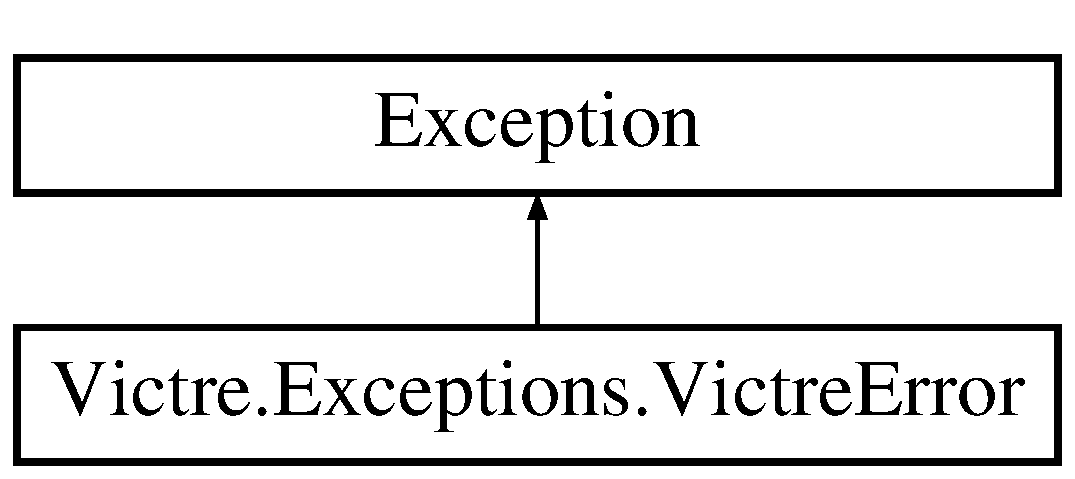
\includegraphics[height=2.000000cm]{classVictre_1_1Exceptions_1_1VictreError}
\end{center}
\end{figure}


\subsection{Detailed Description}
\begin{DoxyVerb}Exception raised for errors in the pipeline.\end{DoxyVerb}
 

The documentation for this class was generated from the following file\-:\begin{DoxyCompactItemize}
\item 
Victre/\hyperlink{Exceptions_8py}{Exceptions.\-py}\end{DoxyCompactItemize}

\chapter{File Documentation}
\hypertarget{get__average__lesion_8py}{\section{get\-\_\-average\-\_\-lesion.\-py File Reference}
\label{get__average__lesion_8py}\index{get\-\_\-average\-\_\-lesion.\-py@{get\-\_\-average\-\_\-lesion.\-py}}
}
\subsection*{Namespaces}
\begin{DoxyCompactItemize}
\item 
\hyperlink{namespaceget__average__lesion}{get\-\_\-average\-\_\-lesion}
\end{DoxyCompactItemize}
\subsection*{Functions}
\begin{DoxyCompactItemize}
\item 
def \hyperlink{namespaceget__average__lesion_a6fa4030a8ff4bd77b404c5c5fe1dcba0}{get\-\_\-average\-\_\-lesion.\-get\-\_\-folder\-\_\-contents}
\end{DoxyCompactItemize}
\subsection*{Variables}
\begin{DoxyCompactItemize}
\item 
dictionary \hyperlink{namespaceget__average__lesion_a04e4f7fdef2b31493b5aab71ddf47d7f}{get\-\_\-average\-\_\-lesion.\-lesion\-\_\-str}
\item 
tuple \hyperlink{namespaceget__average__lesion_a18dd42d421835ddf04df21748b1fbd97}{get\-\_\-average\-\_\-lesion.\-phantoms} = get\-\_\-folder\-\_\-contents(\char`\"{}results\char`\"{})
\item 
dictionary \hyperlink{namespaceget__average__lesion_a1fd4bf63fb19d5891e9e0d3390074201}{get\-\_\-average\-\_\-lesion.\-mean}
\item 
int \hyperlink{namespaceget__average__lesion_aa8eb6c12f2c638c3c97b5cbb4f7aa6b0}{get\-\_\-average\-\_\-lesion.\-num\-\_\-cases} = 3
\item 
tuple \hyperlink{namespaceget__average__lesion_af4a292c67ad6c19a4faf0f86f5aa0f45}{get\-\_\-average\-\_\-lesion.\-rois} = h5py.\-File(ph + \char`\"{}/R\-O\-Is.\-h5\char`\"{}, \char`\"{}r\char`\"{})
\end{DoxyCompactItemize}

\hypertarget{run__pipeline_8py}{\section{run\-\_\-pipeline.\-py File Reference}
\label{run__pipeline_8py}\index{run\-\_\-pipeline.\-py@{run\-\_\-pipeline.\-py}}
}
\subsection*{Namespaces}
\begin{DoxyCompactItemize}
\item 
\hyperlink{namespacerun__pipeline}{run\-\_\-pipeline}
\end{DoxyCompactItemize}
\subsection*{Variables}
\begin{DoxyCompactItemize}
\item 
string \hyperlink{namespacerun__pipeline_aa14c4b2755be317ff6b122e4e340e3ad}{run\-\_\-pipeline.\-hpc\-\_\-cluster\-\_\-ip} = \char`\"{}192.\-168.\-45.\-21\char`\"{}
\item 
string \hyperlink{namespacerun__pipeline_ad2c440e7163ff7674972217024c82f44}{run\-\_\-pipeline.\-phantoms\-\_\-folder} = \char`\"{}/gpfs\-\_\-projects/V\-I\-C\-T\-R\-E/pivotal/phantoms/with\-Lesion/\char`\"{}
\item 
string \hyperlink{namespacerun__pipeline_ae61cb02024dfca7d93506ffb8033e069}{run\-\_\-pipeline.\-density} = \char`\"{}dense\char`\"{}
\item 
tuple \hyperlink{namespacerun__pipeline_a15bae38d22aeec6a0d47fa8cade55406}{run\-\_\-pipeline.\-all\-\_\-seeds} = np.\-loadtxt(phantoms\-\_\-folder + density + \char`\"{}/seeds.\-txt\char`\"{})
\item 
list \hyperlink{namespacerun__pipeline_ae33763f2d174b8a12c1a4d6de9c514d3}{run\-\_\-pipeline.\-lesion\-\_\-only\-\_\-materials}
\item 
string \hyperlink{namespacerun__pipeline_ab0c872cc0ac374f364881c1b8c53be2f}{run\-\_\-pipeline.\-spectrum\-\_\-file} = \char`\"{}./Victre/projection/spectrum/W28k\-Vp\-\_\-\-Rh50um\-\_\-\-Be1mm.\-spc\char`\"{}
\item 
list \hyperlink{namespacerun__pipeline_a0ea10c437dacefc9eb6e69b098f7124d}{run\-\_\-pipeline.\-seed} = all\-\_\-seeds\mbox{[}n\mbox{]}
\item 
\hyperlink{namespacerun__pipeline_a52ad572b0cc10acfe4c6f92accf792c8}{run\-\_\-pipeline.\-phantom\-\_\-file} = phantoms\-\_\-folder+density+\textbackslash{}
\item 
tuple \hyperlink{namespacerun__pipeline_a27b743dac5fef240f9c04a8664ebe49c}{run\-\_\-pipeline.\-pline}
\item 
tuple \hyperlink{namespacerun__pipeline_a6b679545160329ef5ae04905e0fc0f70}{run\-\_\-pipeline.\-vx\-\_\-locations}
\item 
string \hyperlink{namespacerun__pipeline_abaa1ba9de8ccf7d14b2ca397db5de9e9}{run\-\_\-pipeline.\-mhd\-\_\-file} = phantoms\-\_\-folder+density+\char`\"{}/pc\-\_\-\{\-:d\}\-\_\-crop.\-mhd\char`\"{}
\item 
\hyperlink{namespacerun__pipeline_a82244d07ac01d28c7380290c904cadd7}{run\-\_\-pipeline.\-offset} = None
\item 
tuple \hyperlink{namespacerun__pipeline_aaaa6fb70bbde47bf610f101b1c7365ba}{run\-\_\-pipeline.\-line} = f.\-readline()
\item 
dictionary \hyperlink{namespacerun__pipeline_acbbe35ae536f40bcd740b4fa98cd53a1}{run\-\_\-pipeline.\-roi\-\_\-sizes}
\end{DoxyCompactItemize}

\hypertarget{run__pipeline__lesionsizes_8py}{\section{run\-\_\-pipeline\-\_\-lesionsizes.\-py File Reference}
\label{run__pipeline__lesionsizes_8py}\index{run\-\_\-pipeline\-\_\-lesionsizes.\-py@{run\-\_\-pipeline\-\_\-lesionsizes.\-py}}
}
\subsection*{Namespaces}
\begin{DoxyCompactItemize}
\item 
\hyperlink{namespacerun__pipeline__lesionsizes}{run\-\_\-pipeline\-\_\-lesionsizes}
\end{DoxyCompactItemize}
\subsection*{Variables}
\begin{DoxyCompactItemize}
\item 
tuple \hyperlink{namespacerun__pipeline__lesionsizes_a275196213a52b483bde36a8d8b8535cb}{run\-\_\-pipeline\-\_\-lesionsizes.\-parser}
\item 
string \hyperlink{namespacerun__pipeline__lesionsizes_aa88ad88d9cf23592a308b4d4e2ed6ebf}{run\-\_\-pipeline\-\_\-lesionsizes.\-help} = 'Size for the spiculated mass'
\item 
tuple \hyperlink{namespacerun__pipeline__lesionsizes_ae091ae8eef37ab6c53b0409575d19343}{run\-\_\-pipeline\-\_\-lesionsizes.\-lesion\-\_\-size} = parser.\-parse\-\_\-args()
\item 
string \hyperlink{namespacerun__pipeline__lesionsizes_a459355f58091ae51752cbc1b81939a7d}{run\-\_\-pipeline\-\_\-lesionsizes.\-hpc\-\_\-cluster\-\_\-ip} = \char`\"{}192.\-168.\-45.\-21\char`\"{}
\item 
string \hyperlink{namespacerun__pipeline__lesionsizes_a121e580b0ae55595847533bd0f4c9250}{run\-\_\-pipeline\-\_\-lesionsizes.\-phantoms\-\_\-folder} = \char`\"{}/gpfs\-\_\-projects/V\-I\-C\-T\-R\-E/pivotal/phantoms/with\-Lesion/\char`\"{}
\item 
string \hyperlink{namespacerun__pipeline__lesionsizes_ae2a3f1b39ec7dc28c3aa3bc223432ba8}{run\-\_\-pipeline\-\_\-lesionsizes.\-density} = \char`\"{}dense\char`\"{}
\item 
int \hyperlink{namespacerun__pipeline__lesionsizes_a23bb2caa24e95d5ce8622ae343b0035f}{run\-\_\-pipeline\-\_\-lesionsizes.\-num\-\_\-cases} = 3
\item 
tuple \hyperlink{namespacerun__pipeline__lesionsizes_a17e351f66c99883c1fc46e398ddb89db}{run\-\_\-pipeline\-\_\-lesionsizes.\-all\-\_\-seeds} = np.\-loadtxt(phantoms\-\_\-folder + density + \char`\"{}/seeds.\-txt\char`\"{})
\item 
list \hyperlink{namespacerun__pipeline__lesionsizes_aba8698213c56a7ecc0806eb68c010d63}{run\-\_\-pipeline\-\_\-lesionsizes.\-lesion\-\_\-only\-\_\-materials}
\item 
string \hyperlink{namespacerun__pipeline__lesionsizes_aa2e480913d7171fd2b0c89520bcec773}{run\-\_\-pipeline\-\_\-lesionsizes.\-spectrum\-\_\-file} = \char`\"{}./Victre/projection/spectrum/W28k\-Vp\-\_\-\-Rh50um\-\_\-\-Be1mm\-\_\-\-Al2mm\-\_\-\-M\-T\-F.\-spc\char`\"{}
\item 
list \hyperlink{namespacerun__pipeline__lesionsizes_ae359043ae5c4f2c1d8f12c0cdbffb932}{run\-\_\-pipeline\-\_\-lesionsizes.\-seed} = all\-\_\-seeds\mbox{[}n\mbox{]}
\item 
\hyperlink{namespacerun__pipeline__lesionsizes_aa31734859d313f521c7643f1db6be86c}{run\-\_\-pipeline\-\_\-lesionsizes.\-phantom\-\_\-file} = phantoms\-\_\-folder+density+\textbackslash{}
\item 
string \hyperlink{namespacerun__pipeline__lesionsizes_a6036549ef880af11d13c9e0c5d2c001a}{run\-\_\-pipeline\-\_\-lesionsizes.\-lesion\-\_\-file} = \char`\"{}lesions/spiculated/mass\-\_\--\/308854003\-\_\-size\{\-:.\-2f\}.\-h5\char`\"{}
\item 
tuple \hyperlink{namespacerun__pipeline__lesionsizes_ac13a2bd6cea7d4d8155376ddaf1ba751}{run\-\_\-pipeline\-\_\-lesionsizes.\-pline}
\item 
dictionary \hyperlink{namespacerun__pipeline__lesionsizes_a3b75350f1aa1a1b47aa8ef34a06809db}{run\-\_\-pipeline\-\_\-lesionsizes.\-roi\-\_\-sizes}
\item 
int \hyperlink{namespacerun__pipeline__lesionsizes_a8e812d3e5e9a02e87801a5fcdd32c268}{run\-\_\-pipeline\-\_\-lesionsizes.\-n} = 4
\end{DoxyCompactItemize}

\hypertarget{test__pipeline_8py}{\section{test\-\_\-pipeline.\-py File Reference}
\label{test__pipeline_8py}\index{test\-\_\-pipeline.\-py@{test\-\_\-pipeline.\-py}}
}
\subsection*{Namespaces}
\begin{DoxyCompactItemize}
\item 
\hyperlink{namespacetest__pipeline}{test\-\_\-pipeline}
\end{DoxyCompactItemize}
\subsection*{Variables}
\begin{DoxyCompactItemize}
\item 
string \hyperlink{namespacetest__pipeline_af92fee384c18b13c6673a89759d43ed0}{test\-\_\-pipeline.\-hpc\-\_\-cluster\-\_\-ip} = \char`\"{}192.\-168.\-45.\-21\char`\"{}
\item 
string \hyperlink{namespacetest__pipeline_a5a533cd65e06752395913aef099f6f3a}{test\-\_\-pipeline.\-phantoms\-\_\-folder} = \char`\"{}/gpfs\-\_\-projects/V\-I\-C\-T\-R\-E/pivotal/phantoms/with\-Lesion/\char`\"{}
\item 
string \hyperlink{namespacetest__pipeline_ae1187c73a8652306ffcb6026d1c447a9}{test\-\_\-pipeline.\-density} = \char`\"{}dense\char`\"{}
\item 
int \hyperlink{namespacetest__pipeline_a2cc55609849787d81000c76439d285af}{test\-\_\-pipeline.\-seed} = 2132574818
\item 
string \hyperlink{namespacetest__pipeline_a04ba5a1d7ea995de9393c50eb14ef9ad}{test\-\_\-pipeline.\-spectrum\-\_\-file} = \char`\"{}./Victre/projection/spectrum/W28k\-Vp\-\_\-\-Rh50um\-\_\-\-Be1mm.\-spc\char`\"{}
\item 
list \hyperlink{namespacetest__pipeline_a9b60cd1b189b1d4b7ed5d792e12598db}{test\-\_\-pipeline.\-lesion\-\_\-only\-\_\-materials}
\item 
string \hyperlink{namespacetest__pipeline_a12b71fc499f0a1951e42b754b6cfa198}{test\-\_\-pipeline.\-phantom\-\_\-file} = phantoms\-\_\-folder+density+\char`\"{}/pcl\-\_\-\{\-:d\}\-\_\-crop.\-raw.\-gz\char`\"{}
\item 
tuple \hyperlink{namespacetest__pipeline_a4f34ebd50c5400c94a3b33124629e2fe}{test\-\_\-pipeline.\-pline}
\item 
tuple \hyperlink{namespacetest__pipeline_a0891497d3339772fa64ecb2ef3816a8a}{test\-\_\-pipeline.\-vx\-\_\-locations}
\item 
string \hyperlink{namespacetest__pipeline_ae843f1cf40718b92abe9429113865859}{test\-\_\-pipeline.\-mhd\-\_\-file} = phantoms\-\_\-folder+density+\char`\"{}/pc\-\_\-\{\-:d\}\-\_\-crop.\-mhd\char`\"{}
\item 
\hyperlink{namespacetest__pipeline_a0adaf87bfe7dc26e1a0d89f220fb981e}{test\-\_\-pipeline.\-offset} = None
\item 
tuple \hyperlink{namespacetest__pipeline_ae549bb444ef90158d4f47e0c3f8a17d0}{test\-\_\-pipeline.\-line} = f.\-readline()
\item 
dictionary \hyperlink{namespacetest__pipeline_ac3f90bba6b3ba7eb9c6c5fbf56f3f540}{test\-\_\-pipeline.\-roi\-\_\-sizes}
\end{DoxyCompactItemize}

\hypertarget{test__spiculated_8py}{\section{test\-\_\-spiculated.\-py File Reference}
\label{test__spiculated_8py}\index{test\-\_\-spiculated.\-py@{test\-\_\-spiculated.\-py}}
}
\subsection*{Namespaces}
\begin{DoxyCompactItemize}
\item 
\hyperlink{namespacetest__spiculated}{test\-\_\-spiculated}
\end{DoxyCompactItemize}
\subsection*{Variables}
\begin{DoxyCompactItemize}
\item 
string \hyperlink{namespacetest__spiculated_aff5d6f1f85c625e33f5d9c0781bdcabf}{test\-\_\-spiculated.\-hpc\-\_\-cluster\-\_\-ip} = \char`\"{}192.\-168.\-45.\-21\char`\"{}
\item 
string \hyperlink{namespacetest__spiculated_a8e2ee47dc71ed73ef801fe300660add5}{test\-\_\-spiculated.\-phantoms\-\_\-folder} = \char`\"{}/gpfs\-\_\-projects/V\-I\-C\-T\-R\-E/pivotal/phantoms/with\-Lesion/\char`\"{}
\item 
string \hyperlink{namespacetest__spiculated_a058a57e76535b7d35038bffbda8fda91}{test\-\_\-spiculated.\-density} = \char`\"{}dense\char`\"{}
\item 
int \hyperlink{namespacetest__spiculated_ae23883f2f949cd553bd4b1df786aefce}{test\-\_\-spiculated.\-seed} = 2132574818
\item 
string \hyperlink{namespacetest__spiculated_a38dbe89cf6d710045fcb1f252ce6db10}{test\-\_\-spiculated.\-phantom\-\_\-file} = phantoms\-\_\-folder+density+\char`\"{}/pc\-\_\-\{\-:d\}\-\_\-crop.\-raw.\-gz\char`\"{}
\item 
float \hyperlink{namespacetest__spiculated_a40ff806ed0a1985c23f9ee4d5ee829de}{test\-\_\-spiculated.\-size} = 0.\-5
\item 
string \hyperlink{namespacetest__spiculated_ac19b4dd28e8af37f75bf2ec1ecb23c62}{test\-\_\-spiculated.\-lesion\-\_\-file} = \char`\"{}lesions/spiculated/mass\-\_\--\/308854003\-\_\-size\{\-:.\-2f\}.\-h5\char`\"{}
\item 
list \hyperlink{namespacetest__spiculated_ab3f4da20a41fe314d5da3e3ded84fc6f}{test\-\_\-spiculated.\-lesion\-\_\-only\-\_\-materials}
\item 
tuple \hyperlink{namespacetest__spiculated_a2691d025d2f4ab43907a58fd9bbf3c50}{test\-\_\-spiculated.\-pline}
\item 
dictionary \hyperlink{namespacetest__spiculated_aee77941f94eca1ddc6507a6dc644320e}{test\-\_\-spiculated.\-roi\-\_\-sizes}
\item 
int \hyperlink{namespacetest__spiculated_a6d4fc5a3e76208ad33c81d7bffb36de5}{test\-\_\-spiculated.\-n} = 2
\end{DoxyCompactItemize}

\hypertarget{____init_____8py}{\section{Victre/\-\_\-\-\_\-init\-\_\-\-\_\-.py File Reference}
\label{____init_____8py}\index{Victre/\-\_\-\-\_\-init\-\_\-\-\_\-.\-py@{Victre/\-\_\-\-\_\-init\-\_\-\-\_\-.\-py}}
}
\subsection*{Namespaces}
\begin{DoxyCompactItemize}
\item 
\hyperlink{namespaceVictre}{Victre}
\end{DoxyCompactItemize}

\hypertarget{breastMass_8cxx}{\section{Victre/breast\-Mass/breast\-Mass.cxx File Reference}
\label{breastMass_8cxx}\index{Victre/breast\-Mass/breast\-Mass.\-cxx@{Victre/breast\-Mass/breast\-Mass.\-cxx}}
}


breast\-Mass main source file  


{\ttfamily \#include \char`\"{}breast\-Mass.\-hxx\char`\"{}}\\*
\subsection*{Classes}
\begin{DoxyCompactItemize}
\item 
struct \hyperlink{structperturb}{perturb}
\end{DoxyCompactItemize}
\subsection*{Functions}
\begin{DoxyCompactItemize}
\item 
int \hyperlink{breastMass_8cxx_a0ddf1224851353fc92bfbff6f499fa97}{main} (int argc, char $\ast$argv\mbox{[}$\,$\mbox{]})
\item 
void \hyperlink{breastMass_8cxx_a0ab6492def78a98409b7b64d2dedee18}{create\-Branch} (double r, double theta, double phi, double theta\-Dir, double phi\-Dir, double rad, double len, double cont\-Prob, double gam, vtk\-Image\-Data $\ast$mass, vtk\-Minimal\-Standard\-Random\-Sequence $\ast$rgen, vtk\-Box\-Mueller\-Random\-Sequence $\ast$r\-Norm\-Gen, po\-::variables\-\_\-map vm)
\end{DoxyCompactItemize}


\subsection{Detailed Description}
breast\-Mass main source file \begin{DoxyAuthor}{Author}
Christian G. Graff 
\end{DoxyAuthor}
\begin{DoxyVersion}{Version}
1.\-0 
\end{DoxyVersion}
\begin{DoxyDate}{Date}
2018
\end{DoxyDate}
based on \char`\"{}\-A computational model to generate simulated three-\/dimensional breast masses\char`\"{} Sisternes et al., Med. Phys 42(2) 2015.

\begin{DoxyCopyright}{Copyright}
To the extent possible under law, the author(s) have dedicated all copyright and related and neighboring rights to this software to the public domain worldwide. This software is distributed without any warranty. You should have received a copy of the C\-C0 Public Domain Dedication along with this software. If not, see \href{http://creativecommons.org/publicdomain/zero/1.0/}{\tt http\-://creativecommons.\-org/publicdomain/zero/1.\-0/}. 
\end{DoxyCopyright}


\subsection{Function Documentation}
\hypertarget{breastMass_8cxx_a0ab6492def78a98409b7b64d2dedee18}{\index{breast\-Mass.\-cxx@{breast\-Mass.\-cxx}!create\-Branch@{create\-Branch}}
\index{create\-Branch@{create\-Branch}!breastMass.cxx@{breast\-Mass.\-cxx}}
\subsubsection[{create\-Branch}]{\setlength{\rightskip}{0pt plus 5cm}void create\-Branch (
\begin{DoxyParamCaption}
\item[{double}]{r, }
\item[{double}]{theta, }
\item[{double}]{phi, }
\item[{double}]{theta\-Dir, }
\item[{double}]{phi\-Dir, }
\item[{double}]{rad, }
\item[{double}]{len, }
\item[{double}]{cont\-Prob, }
\item[{double}]{gam, }
\item[{vtk\-Image\-Data $\ast$}]{mass, }
\item[{vtk\-Minimal\-Standard\-Random\-Sequence $\ast$}]{rgen, }
\item[{vtk\-Box\-Mueller\-Random\-Sequence $\ast$}]{r\-Norm\-Gen, }
\item[{po\-::variables\-\_\-map}]{vm}
\end{DoxyParamCaption}
)}}\label{breastMass_8cxx_a0ab6492def78a98409b7b64d2dedee18}
\hypertarget{breastMass_8cxx_a0ddf1224851353fc92bfbff6f499fa97}{\index{breast\-Mass.\-cxx@{breast\-Mass.\-cxx}!main@{main}}
\index{main@{main}!breastMass.cxx@{breast\-Mass.\-cxx}}
\subsubsection[{main}]{\setlength{\rightskip}{0pt plus 5cm}int main (
\begin{DoxyParamCaption}
\item[{int}]{argc, }
\item[{char $\ast$}]{argv\mbox{[}$\,$\mbox{]}}
\end{DoxyParamCaption}
)}}\label{breastMass_8cxx_a0ddf1224851353fc92bfbff6f499fa97}

\hypertarget{breastMass_8hxx}{\section{Victre/breast\-Mass/breast\-Mass.hxx File Reference}
\label{breastMass_8hxx}\index{Victre/breast\-Mass/breast\-Mass.\-hxx@{Victre/breast\-Mass/breast\-Mass.\-hxx}}
}


breast\-Mass header file  


{\ttfamily \#include $<$boost/math/special\-\_\-functions/spherical\-\_\-harmonic.\-hpp$>$}\\*
{\ttfamily \#include $<$boost/program\-\_\-options.\-hpp$>$}\\*
{\ttfamily \#include $<$iostream$>$}\\*
{\ttfamily \#include $<$math.\-h$>$}\\*
{\ttfamily \#include $<$unistd.\-h$>$}\\*
{\ttfamily \#include $<$sys/stat.\-h$>$}\\*
{\ttfamily \#include $<$omp.\-h$>$}\\*
{\ttfamily \#include $<$vtk\-Version.\-h$>$}\\*
{\ttfamily \#include $<$vtk\-Smart\-Pointer.\-h$>$}\\*
{\ttfamily \#include $<$vtk\-Math.\-h$>$}\\*
{\ttfamily \#include $<$vtk\-P\-N\-G\-Writer.\-h$>$}\\*
{\ttfamily \#include $<$vtk\-Image\-Data.\-h$>$}\\*
{\ttfamily \#include $<$vtk\-X\-M\-L\-Image\-Data\-Writer.\-h$>$}\\*
{\ttfamily \#include $<$vtk\-Minimal\-Standard\-Random\-Sequence.\-h$>$}\\*
{\ttfamily \#include $<$vtk\-Box\-Mueller\-Random\-Sequence.\-h$>$}\\*
{\ttfamily \#include $<$vtk\-Image\-Interpolator.\-h$>$}\\*
\subsection*{Functions}
\begin{DoxyCompactItemize}
\item 
void \hyperlink{breastMass_8hxx_a7169a38c69ba3f24d4be9799e8b72085}{create\-Branch} (double, double, double, double, double, double, double, double, double, vtk\-Image\-Data $\ast$, vtk\-Minimal\-Standard\-Random\-Sequence $\ast$, vtk\-Box\-Mueller\-Random\-Sequence $\ast$, boost\-::program\-\_\-options\-::variables\-\_\-map)
\end{DoxyCompactItemize}


\subsection{Detailed Description}
breast\-Mass header file \begin{DoxyAuthor}{Author}
Christian G. Graff 
\end{DoxyAuthor}
\begin{DoxyVersion}{Version}
1.\-0 
\end{DoxyVersion}
\begin{DoxyDate}{Date}
2018
\end{DoxyDate}
\begin{DoxyCopyright}{Copyright}
To the extent possible under law, the author(s) have dedicated all copyright and related and neighboring rights to this software to the public domain worldwide. This software is distributed without any warranty. You should have received a copy of the C\-C0 Public Domain Dedication along with this software. If not, see \href{http://creativecommons.org/publicdomain/zero/1.0/}{\tt http\-://creativecommons.\-org/publicdomain/zero/1.\-0/}. 
\end{DoxyCopyright}


\subsection{Function Documentation}
\hypertarget{breastMass_8hxx_a7169a38c69ba3f24d4be9799e8b72085}{\index{breast\-Mass.\-hxx@{breast\-Mass.\-hxx}!create\-Branch@{create\-Branch}}
\index{create\-Branch@{create\-Branch}!breastMass.hxx@{breast\-Mass.\-hxx}}
\subsubsection[{create\-Branch}]{\setlength{\rightskip}{0pt plus 5cm}void create\-Branch (
\begin{DoxyParamCaption}
\item[{double}]{, }
\item[{double}]{, }
\item[{double}]{, }
\item[{double}]{, }
\item[{double}]{, }
\item[{double}]{, }
\item[{double}]{, }
\item[{double}]{, }
\item[{double}]{, }
\item[{vtk\-Image\-Data $\ast$}]{, }
\item[{vtk\-Minimal\-Standard\-Random\-Sequence $\ast$}]{, }
\item[{vtk\-Box\-Mueller\-Random\-Sequence $\ast$}]{, }
\item[{boost\-::program\-\_\-options\-::variables\-\_\-map}]{}
\end{DoxyParamCaption}
)}}\label{breastMass_8hxx_a7169a38c69ba3f24d4be9799e8b72085}

\hypertarget{CMakeCCompilerId_8c}{\section{Victre/breast\-Mass/\-C\-Make\-Files/2.8.12.2/\-Compiler\-Id\-C/\-C\-Make\-C\-Compiler\-Id.c File Reference}
\label{CMakeCCompilerId_8c}\index{Victre/breast\-Mass/\-C\-Make\-Files/2.\-8.\-12.\-2/\-Compiler\-Id\-C/\-C\-Make\-C\-Compiler\-Id.\-c@{Victre/breast\-Mass/\-C\-Make\-Files/2.\-8.\-12.\-2/\-Compiler\-Id\-C/\-C\-Make\-C\-Compiler\-Id.\-c}}
}
\subsection*{Macros}
\begin{DoxyCompactItemize}
\item 
\#define \hyperlink{CMakeCCompilerId_8c_a81dee0709ded976b2e0319239f72d174}{C\-O\-M\-P\-I\-L\-E\-R\-\_\-\-I\-D}~\char`\"{}\char`\"{}
\item 
\#define \hyperlink{CMakeCCompilerId_8c_adbc5372f40838899018fadbc89bd588b}{P\-L\-A\-T\-F\-O\-R\-M\-\_\-\-I\-D}~\char`\"{}\char`\"{}
\item 
\#define \hyperlink{CMakeCCompilerId_8c_aba35d0d200deaeb06aee95ca297acb28}{A\-R\-C\-H\-I\-T\-E\-C\-T\-U\-R\-E\-\_\-\-I\-D}~\char`\"{}\char`\"{}
\item 
\#define \hyperlink{CMakeCCompilerId_8c_ad1280362da42492bbc11aa78cbf776ad}{D\-E\-C}(n)
\item 
\#define \hyperlink{CMakeCCompilerId_8c_a46d5d95daa1bef867bd0179594310ed5}{H\-E\-X}(n)
\end{DoxyCompactItemize}
\subsection*{Functions}
\begin{DoxyCompactItemize}
\item 
int \hyperlink{CMakeCCompilerId_8c_a0ddf1224851353fc92bfbff6f499fa97}{main} (int argc, char $\ast$argv\mbox{[}$\,$\mbox{]})
\end{DoxyCompactItemize}
\subsection*{Variables}
\begin{DoxyCompactItemize}
\item 
char const $\ast$ \hyperlink{CMakeCCompilerId_8c_a4b0efeb7a5d59313986b3a0390f050f6}{info\-\_\-compiler} = \char`\"{}I\-N\-F\-O\char`\"{} \char`\"{}\-:\char`\"{} \char`\"{}compiler\mbox{[}\char`\"{} C\-O\-M\-P\-I\-L\-E\-R\-\_\-\-I\-D \char`\"{}\mbox{]}\char`\"{}
\item 
char const $\ast$ \hyperlink{CMakeCCompilerId_8c_a2321403dee54ee23f0c2fa849c60f7d4}{info\-\_\-platform} = \char`\"{}I\-N\-F\-O\char`\"{} \char`\"{}\-:\char`\"{} \char`\"{}platform\mbox{[}\char`\"{} P\-L\-A\-T\-F\-O\-R\-M\-\_\-\-I\-D \char`\"{}\mbox{]}\char`\"{}
\item 
char const $\ast$ \hyperlink{CMakeCCompilerId_8c_a59647e99d304ed33b15cb284c27ed391}{info\-\_\-arch} = \char`\"{}I\-N\-F\-O\char`\"{} \char`\"{}\-:\char`\"{} \char`\"{}arch\mbox{[}\char`\"{} A\-R\-C\-H\-I\-T\-E\-C\-T\-U\-R\-E\-\_\-\-I\-D \char`\"{}\mbox{]}\char`\"{}
\end{DoxyCompactItemize}


\subsection{Macro Definition Documentation}
\hypertarget{CMakeCCompilerId_8c_aba35d0d200deaeb06aee95ca297acb28}{\index{C\-Make\-C\-Compiler\-Id.\-c@{C\-Make\-C\-Compiler\-Id.\-c}!A\-R\-C\-H\-I\-T\-E\-C\-T\-U\-R\-E\-\_\-\-I\-D@{A\-R\-C\-H\-I\-T\-E\-C\-T\-U\-R\-E\-\_\-\-I\-D}}
\index{A\-R\-C\-H\-I\-T\-E\-C\-T\-U\-R\-E\-\_\-\-I\-D@{A\-R\-C\-H\-I\-T\-E\-C\-T\-U\-R\-E\-\_\-\-I\-D}!CMakeCCompilerId.c@{C\-Make\-C\-Compiler\-Id.\-c}}
\subsubsection[{A\-R\-C\-H\-I\-T\-E\-C\-T\-U\-R\-E\-\_\-\-I\-D}]{\setlength{\rightskip}{0pt plus 5cm}\#define A\-R\-C\-H\-I\-T\-E\-C\-T\-U\-R\-E\-\_\-\-I\-D~\char`\"{}\char`\"{}}}\label{CMakeCCompilerId_8c_aba35d0d200deaeb06aee95ca297acb28}
\hypertarget{CMakeCCompilerId_8c_a81dee0709ded976b2e0319239f72d174}{\index{C\-Make\-C\-Compiler\-Id.\-c@{C\-Make\-C\-Compiler\-Id.\-c}!C\-O\-M\-P\-I\-L\-E\-R\-\_\-\-I\-D@{C\-O\-M\-P\-I\-L\-E\-R\-\_\-\-I\-D}}
\index{C\-O\-M\-P\-I\-L\-E\-R\-\_\-\-I\-D@{C\-O\-M\-P\-I\-L\-E\-R\-\_\-\-I\-D}!CMakeCCompilerId.c@{C\-Make\-C\-Compiler\-Id.\-c}}
\subsubsection[{C\-O\-M\-P\-I\-L\-E\-R\-\_\-\-I\-D}]{\setlength{\rightskip}{0pt plus 5cm}\#define C\-O\-M\-P\-I\-L\-E\-R\-\_\-\-I\-D~\char`\"{}\char`\"{}}}\label{CMakeCCompilerId_8c_a81dee0709ded976b2e0319239f72d174}
\hypertarget{CMakeCCompilerId_8c_ad1280362da42492bbc11aa78cbf776ad}{\index{C\-Make\-C\-Compiler\-Id.\-c@{C\-Make\-C\-Compiler\-Id.\-c}!D\-E\-C@{D\-E\-C}}
\index{D\-E\-C@{D\-E\-C}!CMakeCCompilerId.c@{C\-Make\-C\-Compiler\-Id.\-c}}
\subsubsection[{D\-E\-C}]{\setlength{\rightskip}{0pt plus 5cm}\#define D\-E\-C(
\begin{DoxyParamCaption}
\item[{}]{n}
\end{DoxyParamCaption}
)}}\label{CMakeCCompilerId_8c_ad1280362da42492bbc11aa78cbf776ad}
{\bfseries Value\-:}
\begin{DoxyCode}
(\textcolor{charliteral}{'0'} + (((\hyperlink{namespacerun__pipeline__lesionsizes_a8e812d3e5e9a02e87801a5fcdd32c268}{n}) / 10000000)%10)), \(\backslash\)
  (\textcolor{charliteral}{'0'} + (((\hyperlink{namespacerun__pipeline__lesionsizes_a8e812d3e5e9a02e87801a5fcdd32c268}{n}) / 1000000)%10)),  \(\backslash\)
  (\textcolor{charliteral}{'0'} + (((\hyperlink{namespacerun__pipeline__lesionsizes_a8e812d3e5e9a02e87801a5fcdd32c268}{n}) / 100000)%10)),   \(\backslash\)
  (\textcolor{charliteral}{'0'} + (((\hyperlink{namespacerun__pipeline__lesionsizes_a8e812d3e5e9a02e87801a5fcdd32c268}{n}) / 10000)%10)),    \(\backslash\)
  (\textcolor{charliteral}{'0'} + (((\hyperlink{namespacerun__pipeline__lesionsizes_a8e812d3e5e9a02e87801a5fcdd32c268}{n}) / 1000)%10)),     \(\backslash\)
  (\textcolor{charliteral}{'0'} + (((\hyperlink{namespacerun__pipeline__lesionsizes_a8e812d3e5e9a02e87801a5fcdd32c268}{n}) / 100)%10)),      \(\backslash\)
  (\textcolor{charliteral}{'0'} + (((\hyperlink{namespacerun__pipeline__lesionsizes_a8e812d3e5e9a02e87801a5fcdd32c268}{n}) / 10)%10)),       \(\backslash\)
  (\textcolor{charliteral}{'0'} +  ((\hyperlink{namespacerun__pipeline__lesionsizes_a8e812d3e5e9a02e87801a5fcdd32c268}{n}) % 10))
\end{DoxyCode}
\hypertarget{CMakeCCompilerId_8c_a46d5d95daa1bef867bd0179594310ed5}{\index{C\-Make\-C\-Compiler\-Id.\-c@{C\-Make\-C\-Compiler\-Id.\-c}!H\-E\-X@{H\-E\-X}}
\index{H\-E\-X@{H\-E\-X}!CMakeCCompilerId.c@{C\-Make\-C\-Compiler\-Id.\-c}}
\subsubsection[{H\-E\-X}]{\setlength{\rightskip}{0pt plus 5cm}\#define H\-E\-X(
\begin{DoxyParamCaption}
\item[{}]{n}
\end{DoxyParamCaption}
)}}\label{CMakeCCompilerId_8c_a46d5d95daa1bef867bd0179594310ed5}
{\bfseries Value\-:}
\begin{DoxyCode}
(\textcolor{charliteral}{'0'} + ((\hyperlink{namespacerun__pipeline__lesionsizes_a8e812d3e5e9a02e87801a5fcdd32c268}{n})>>28 & 0xF)), \(\backslash\)
  (\textcolor{charliteral}{'0'} + ((\hyperlink{namespacerun__pipeline__lesionsizes_a8e812d3e5e9a02e87801a5fcdd32c268}{n})>>24 & 0xF)), \(\backslash\)
  (\textcolor{charliteral}{'0'} + ((\hyperlink{namespacerun__pipeline__lesionsizes_a8e812d3e5e9a02e87801a5fcdd32c268}{n})>>20 & 0xF)), \(\backslash\)
  (\textcolor{charliteral}{'0'} + ((\hyperlink{namespacerun__pipeline__lesionsizes_a8e812d3e5e9a02e87801a5fcdd32c268}{n})>>16 & 0xF)), \(\backslash\)
  (\textcolor{charliteral}{'0'} + ((\hyperlink{namespacerun__pipeline__lesionsizes_a8e812d3e5e9a02e87801a5fcdd32c268}{n})>>12 & 0xF)), \(\backslash\)
  (\textcolor{charliteral}{'0'} + ((\hyperlink{namespacerun__pipeline__lesionsizes_a8e812d3e5e9a02e87801a5fcdd32c268}{n})>>8  & 0xF)), \(\backslash\)
  (\textcolor{charliteral}{'0'} + ((\hyperlink{namespacerun__pipeline__lesionsizes_a8e812d3e5e9a02e87801a5fcdd32c268}{n})>>4  & 0xF)), \(\backslash\)
  (\textcolor{charliteral}{'0'} + ((\hyperlink{namespacerun__pipeline__lesionsizes_a8e812d3e5e9a02e87801a5fcdd32c268}{n})     & 0xF))
\end{DoxyCode}
\hypertarget{CMakeCCompilerId_8c_adbc5372f40838899018fadbc89bd588b}{\index{C\-Make\-C\-Compiler\-Id.\-c@{C\-Make\-C\-Compiler\-Id.\-c}!P\-L\-A\-T\-F\-O\-R\-M\-\_\-\-I\-D@{P\-L\-A\-T\-F\-O\-R\-M\-\_\-\-I\-D}}
\index{P\-L\-A\-T\-F\-O\-R\-M\-\_\-\-I\-D@{P\-L\-A\-T\-F\-O\-R\-M\-\_\-\-I\-D}!CMakeCCompilerId.c@{C\-Make\-C\-Compiler\-Id.\-c}}
\subsubsection[{P\-L\-A\-T\-F\-O\-R\-M\-\_\-\-I\-D}]{\setlength{\rightskip}{0pt plus 5cm}\#define P\-L\-A\-T\-F\-O\-R\-M\-\_\-\-I\-D~\char`\"{}\char`\"{}}}\label{CMakeCCompilerId_8c_adbc5372f40838899018fadbc89bd588b}


\subsection{Function Documentation}
\hypertarget{CMakeCCompilerId_8c_a0ddf1224851353fc92bfbff6f499fa97}{\index{C\-Make\-C\-Compiler\-Id.\-c@{C\-Make\-C\-Compiler\-Id.\-c}!main@{main}}
\index{main@{main}!CMakeCCompilerId.c@{C\-Make\-C\-Compiler\-Id.\-c}}
\subsubsection[{main}]{\setlength{\rightskip}{0pt plus 5cm}int main (
\begin{DoxyParamCaption}
\item[{int}]{argc, }
\item[{char $\ast$}]{argv\mbox{[}$\,$\mbox{]}}
\end{DoxyParamCaption}
)}}\label{CMakeCCompilerId_8c_a0ddf1224851353fc92bfbff6f499fa97}


\subsection{Variable Documentation}
\hypertarget{CMakeCCompilerId_8c_a59647e99d304ed33b15cb284c27ed391}{\index{C\-Make\-C\-Compiler\-Id.\-c@{C\-Make\-C\-Compiler\-Id.\-c}!info\-\_\-arch@{info\-\_\-arch}}
\index{info\-\_\-arch@{info\-\_\-arch}!CMakeCCompilerId.c@{C\-Make\-C\-Compiler\-Id.\-c}}
\subsubsection[{info\-\_\-arch}]{\setlength{\rightskip}{0pt plus 5cm}char const$\ast$ info\-\_\-arch = \char`\"{}I\-N\-F\-O\char`\"{} \char`\"{}\-:\char`\"{} \char`\"{}arch\mbox{[}\char`\"{} A\-R\-C\-H\-I\-T\-E\-C\-T\-U\-R\-E\-\_\-\-I\-D \char`\"{}\mbox{]}\char`\"{}}}\label{CMakeCCompilerId_8c_a59647e99d304ed33b15cb284c27ed391}
\hypertarget{CMakeCCompilerId_8c_a4b0efeb7a5d59313986b3a0390f050f6}{\index{C\-Make\-C\-Compiler\-Id.\-c@{C\-Make\-C\-Compiler\-Id.\-c}!info\-\_\-compiler@{info\-\_\-compiler}}
\index{info\-\_\-compiler@{info\-\_\-compiler}!CMakeCCompilerId.c@{C\-Make\-C\-Compiler\-Id.\-c}}
\subsubsection[{info\-\_\-compiler}]{\setlength{\rightskip}{0pt plus 5cm}char const$\ast$ info\-\_\-compiler = \char`\"{}I\-N\-F\-O\char`\"{} \char`\"{}\-:\char`\"{} \char`\"{}compiler\mbox{[}\char`\"{} C\-O\-M\-P\-I\-L\-E\-R\-\_\-\-I\-D \char`\"{}\mbox{]}\char`\"{}}}\label{CMakeCCompilerId_8c_a4b0efeb7a5d59313986b3a0390f050f6}
\hypertarget{CMakeCCompilerId_8c_a2321403dee54ee23f0c2fa849c60f7d4}{\index{C\-Make\-C\-Compiler\-Id.\-c@{C\-Make\-C\-Compiler\-Id.\-c}!info\-\_\-platform@{info\-\_\-platform}}
\index{info\-\_\-platform@{info\-\_\-platform}!CMakeCCompilerId.c@{C\-Make\-C\-Compiler\-Id.\-c}}
\subsubsection[{info\-\_\-platform}]{\setlength{\rightskip}{0pt plus 5cm}char const$\ast$ info\-\_\-platform = \char`\"{}I\-N\-F\-O\char`\"{} \char`\"{}\-:\char`\"{} \char`\"{}platform\mbox{[}\char`\"{} P\-L\-A\-T\-F\-O\-R\-M\-\_\-\-I\-D \char`\"{}\mbox{]}\char`\"{}}}\label{CMakeCCompilerId_8c_a2321403dee54ee23f0c2fa849c60f7d4}

\hypertarget{CMakeCXXCompilerId_8cpp}{\section{Victre/breast\-Mass/\-C\-Make\-Files/2.8.12.2/\-Compiler\-Id\-C\-X\-X/\-C\-Make\-C\-X\-X\-Compiler\-Id.cpp File Reference}
\label{CMakeCXXCompilerId_8cpp}\index{Victre/breast\-Mass/\-C\-Make\-Files/2.\-8.\-12.\-2/\-Compiler\-Id\-C\-X\-X/\-C\-Make\-C\-X\-X\-Compiler\-Id.\-cpp@{Victre/breast\-Mass/\-C\-Make\-Files/2.\-8.\-12.\-2/\-Compiler\-Id\-C\-X\-X/\-C\-Make\-C\-X\-X\-Compiler\-Id.\-cpp}}
}
\subsection*{Macros}
\begin{DoxyCompactItemize}
\item 
\#define \hyperlink{CMakeCXXCompilerId_8cpp_a81dee0709ded976b2e0319239f72d174}{C\-O\-M\-P\-I\-L\-E\-R\-\_\-\-I\-D}~\char`\"{}\char`\"{}
\item 
\#define \hyperlink{CMakeCXXCompilerId_8cpp_adbc5372f40838899018fadbc89bd588b}{P\-L\-A\-T\-F\-O\-R\-M\-\_\-\-I\-D}~\char`\"{}\char`\"{}
\item 
\#define \hyperlink{CMakeCXXCompilerId_8cpp_aba35d0d200deaeb06aee95ca297acb28}{A\-R\-C\-H\-I\-T\-E\-C\-T\-U\-R\-E\-\_\-\-I\-D}~\char`\"{}\char`\"{}
\item 
\#define \hyperlink{CMakeCXXCompilerId_8cpp_ad1280362da42492bbc11aa78cbf776ad}{D\-E\-C}(n)
\item 
\#define \hyperlink{CMakeCXXCompilerId_8cpp_a46d5d95daa1bef867bd0179594310ed5}{H\-E\-X}(n)
\end{DoxyCompactItemize}
\subsection*{Functions}
\begin{DoxyCompactItemize}
\item 
int \hyperlink{CMakeCXXCompilerId_8cpp_a0ddf1224851353fc92bfbff6f499fa97}{main} (int argc, char $\ast$argv\mbox{[}$\,$\mbox{]})
\end{DoxyCompactItemize}
\subsection*{Variables}
\begin{DoxyCompactItemize}
\item 
char const $\ast$ \hyperlink{CMakeCXXCompilerId_8cpp_a4b0efeb7a5d59313986b3a0390f050f6}{info\-\_\-compiler} = \char`\"{}I\-N\-F\-O\char`\"{} \char`\"{}\-:\char`\"{} \char`\"{}compiler\mbox{[}\char`\"{} C\-O\-M\-P\-I\-L\-E\-R\-\_\-\-I\-D \char`\"{}\mbox{]}\char`\"{}
\item 
char const $\ast$ \hyperlink{CMakeCXXCompilerId_8cpp_a2321403dee54ee23f0c2fa849c60f7d4}{info\-\_\-platform} = \char`\"{}I\-N\-F\-O\char`\"{} \char`\"{}\-:\char`\"{} \char`\"{}platform\mbox{[}\char`\"{} P\-L\-A\-T\-F\-O\-R\-M\-\_\-\-I\-D \char`\"{}\mbox{]}\char`\"{}
\item 
char const $\ast$ \hyperlink{CMakeCXXCompilerId_8cpp_a59647e99d304ed33b15cb284c27ed391}{info\-\_\-arch} = \char`\"{}I\-N\-F\-O\char`\"{} \char`\"{}\-:\char`\"{} \char`\"{}arch\mbox{[}\char`\"{} A\-R\-C\-H\-I\-T\-E\-C\-T\-U\-R\-E\-\_\-\-I\-D \char`\"{}\mbox{]}\char`\"{}
\end{DoxyCompactItemize}


\subsection{Macro Definition Documentation}
\hypertarget{CMakeCXXCompilerId_8cpp_aba35d0d200deaeb06aee95ca297acb28}{\index{C\-Make\-C\-X\-X\-Compiler\-Id.\-cpp@{C\-Make\-C\-X\-X\-Compiler\-Id.\-cpp}!A\-R\-C\-H\-I\-T\-E\-C\-T\-U\-R\-E\-\_\-\-I\-D@{A\-R\-C\-H\-I\-T\-E\-C\-T\-U\-R\-E\-\_\-\-I\-D}}
\index{A\-R\-C\-H\-I\-T\-E\-C\-T\-U\-R\-E\-\_\-\-I\-D@{A\-R\-C\-H\-I\-T\-E\-C\-T\-U\-R\-E\-\_\-\-I\-D}!CMakeCXXCompilerId.cpp@{C\-Make\-C\-X\-X\-Compiler\-Id.\-cpp}}
\subsubsection[{A\-R\-C\-H\-I\-T\-E\-C\-T\-U\-R\-E\-\_\-\-I\-D}]{\setlength{\rightskip}{0pt plus 5cm}\#define A\-R\-C\-H\-I\-T\-E\-C\-T\-U\-R\-E\-\_\-\-I\-D~\char`\"{}\char`\"{}}}\label{CMakeCXXCompilerId_8cpp_aba35d0d200deaeb06aee95ca297acb28}
\hypertarget{CMakeCXXCompilerId_8cpp_a81dee0709ded976b2e0319239f72d174}{\index{C\-Make\-C\-X\-X\-Compiler\-Id.\-cpp@{C\-Make\-C\-X\-X\-Compiler\-Id.\-cpp}!C\-O\-M\-P\-I\-L\-E\-R\-\_\-\-I\-D@{C\-O\-M\-P\-I\-L\-E\-R\-\_\-\-I\-D}}
\index{C\-O\-M\-P\-I\-L\-E\-R\-\_\-\-I\-D@{C\-O\-M\-P\-I\-L\-E\-R\-\_\-\-I\-D}!CMakeCXXCompilerId.cpp@{C\-Make\-C\-X\-X\-Compiler\-Id.\-cpp}}
\subsubsection[{C\-O\-M\-P\-I\-L\-E\-R\-\_\-\-I\-D}]{\setlength{\rightskip}{0pt plus 5cm}\#define C\-O\-M\-P\-I\-L\-E\-R\-\_\-\-I\-D~\char`\"{}\char`\"{}}}\label{CMakeCXXCompilerId_8cpp_a81dee0709ded976b2e0319239f72d174}
\hypertarget{CMakeCXXCompilerId_8cpp_ad1280362da42492bbc11aa78cbf776ad}{\index{C\-Make\-C\-X\-X\-Compiler\-Id.\-cpp@{C\-Make\-C\-X\-X\-Compiler\-Id.\-cpp}!D\-E\-C@{D\-E\-C}}
\index{D\-E\-C@{D\-E\-C}!CMakeCXXCompilerId.cpp@{C\-Make\-C\-X\-X\-Compiler\-Id.\-cpp}}
\subsubsection[{D\-E\-C}]{\setlength{\rightskip}{0pt plus 5cm}\#define D\-E\-C(
\begin{DoxyParamCaption}
\item[{}]{n}
\end{DoxyParamCaption}
)}}\label{CMakeCXXCompilerId_8cpp_ad1280362da42492bbc11aa78cbf776ad}
{\bfseries Value\-:}
\begin{DoxyCode}
(\textcolor{charliteral}{'0'} + (((\hyperlink{namespacerun__pipeline__lesionsizes_a8e812d3e5e9a02e87801a5fcdd32c268}{n}) / 10000000)%10)), \(\backslash\)
  (\textcolor{charliteral}{'0'} + (((\hyperlink{namespacerun__pipeline__lesionsizes_a8e812d3e5e9a02e87801a5fcdd32c268}{n}) / 1000000)%10)),  \(\backslash\)
  (\textcolor{charliteral}{'0'} + (((\hyperlink{namespacerun__pipeline__lesionsizes_a8e812d3e5e9a02e87801a5fcdd32c268}{n}) / 100000)%10)),   \(\backslash\)
  (\textcolor{charliteral}{'0'} + (((\hyperlink{namespacerun__pipeline__lesionsizes_a8e812d3e5e9a02e87801a5fcdd32c268}{n}) / 10000)%10)),    \(\backslash\)
  (\textcolor{charliteral}{'0'} + (((\hyperlink{namespacerun__pipeline__lesionsizes_a8e812d3e5e9a02e87801a5fcdd32c268}{n}) / 1000)%10)),     \(\backslash\)
  (\textcolor{charliteral}{'0'} + (((\hyperlink{namespacerun__pipeline__lesionsizes_a8e812d3e5e9a02e87801a5fcdd32c268}{n}) / 100)%10)),      \(\backslash\)
  (\textcolor{charliteral}{'0'} + (((\hyperlink{namespacerun__pipeline__lesionsizes_a8e812d3e5e9a02e87801a5fcdd32c268}{n}) / 10)%10)),       \(\backslash\)
  (\textcolor{charliteral}{'0'} +  ((\hyperlink{namespacerun__pipeline__lesionsizes_a8e812d3e5e9a02e87801a5fcdd32c268}{n}) % 10))
\end{DoxyCode}
\hypertarget{CMakeCXXCompilerId_8cpp_a46d5d95daa1bef867bd0179594310ed5}{\index{C\-Make\-C\-X\-X\-Compiler\-Id.\-cpp@{C\-Make\-C\-X\-X\-Compiler\-Id.\-cpp}!H\-E\-X@{H\-E\-X}}
\index{H\-E\-X@{H\-E\-X}!CMakeCXXCompilerId.cpp@{C\-Make\-C\-X\-X\-Compiler\-Id.\-cpp}}
\subsubsection[{H\-E\-X}]{\setlength{\rightskip}{0pt plus 5cm}\#define H\-E\-X(
\begin{DoxyParamCaption}
\item[{}]{n}
\end{DoxyParamCaption}
)}}\label{CMakeCXXCompilerId_8cpp_a46d5d95daa1bef867bd0179594310ed5}
{\bfseries Value\-:}
\begin{DoxyCode}
(\textcolor{charliteral}{'0'} + ((\hyperlink{namespacerun__pipeline__lesionsizes_a8e812d3e5e9a02e87801a5fcdd32c268}{n})>>28 & 0xF)), \(\backslash\)
  (\textcolor{charliteral}{'0'} + ((\hyperlink{namespacerun__pipeline__lesionsizes_a8e812d3e5e9a02e87801a5fcdd32c268}{n})>>24 & 0xF)), \(\backslash\)
  (\textcolor{charliteral}{'0'} + ((\hyperlink{namespacerun__pipeline__lesionsizes_a8e812d3e5e9a02e87801a5fcdd32c268}{n})>>20 & 0xF)), \(\backslash\)
  (\textcolor{charliteral}{'0'} + ((\hyperlink{namespacerun__pipeline__lesionsizes_a8e812d3e5e9a02e87801a5fcdd32c268}{n})>>16 & 0xF)), \(\backslash\)
  (\textcolor{charliteral}{'0'} + ((\hyperlink{namespacerun__pipeline__lesionsizes_a8e812d3e5e9a02e87801a5fcdd32c268}{n})>>12 & 0xF)), \(\backslash\)
  (\textcolor{charliteral}{'0'} + ((\hyperlink{namespacerun__pipeline__lesionsizes_a8e812d3e5e9a02e87801a5fcdd32c268}{n})>>8  & 0xF)), \(\backslash\)
  (\textcolor{charliteral}{'0'} + ((\hyperlink{namespacerun__pipeline__lesionsizes_a8e812d3e5e9a02e87801a5fcdd32c268}{n})>>4  & 0xF)), \(\backslash\)
  (\textcolor{charliteral}{'0'} + ((\hyperlink{namespacerun__pipeline__lesionsizes_a8e812d3e5e9a02e87801a5fcdd32c268}{n})     & 0xF))
\end{DoxyCode}
\hypertarget{CMakeCXXCompilerId_8cpp_adbc5372f40838899018fadbc89bd588b}{\index{C\-Make\-C\-X\-X\-Compiler\-Id.\-cpp@{C\-Make\-C\-X\-X\-Compiler\-Id.\-cpp}!P\-L\-A\-T\-F\-O\-R\-M\-\_\-\-I\-D@{P\-L\-A\-T\-F\-O\-R\-M\-\_\-\-I\-D}}
\index{P\-L\-A\-T\-F\-O\-R\-M\-\_\-\-I\-D@{P\-L\-A\-T\-F\-O\-R\-M\-\_\-\-I\-D}!CMakeCXXCompilerId.cpp@{C\-Make\-C\-X\-X\-Compiler\-Id.\-cpp}}
\subsubsection[{P\-L\-A\-T\-F\-O\-R\-M\-\_\-\-I\-D}]{\setlength{\rightskip}{0pt plus 5cm}\#define P\-L\-A\-T\-F\-O\-R\-M\-\_\-\-I\-D~\char`\"{}\char`\"{}}}\label{CMakeCXXCompilerId_8cpp_adbc5372f40838899018fadbc89bd588b}


\subsection{Function Documentation}
\hypertarget{CMakeCXXCompilerId_8cpp_a0ddf1224851353fc92bfbff6f499fa97}{\index{C\-Make\-C\-X\-X\-Compiler\-Id.\-cpp@{C\-Make\-C\-X\-X\-Compiler\-Id.\-cpp}!main@{main}}
\index{main@{main}!CMakeCXXCompilerId.cpp@{C\-Make\-C\-X\-X\-Compiler\-Id.\-cpp}}
\subsubsection[{main}]{\setlength{\rightskip}{0pt plus 5cm}int main (
\begin{DoxyParamCaption}
\item[{int}]{argc, }
\item[{char $\ast$}]{argv\mbox{[}$\,$\mbox{]}}
\end{DoxyParamCaption}
)}}\label{CMakeCXXCompilerId_8cpp_a0ddf1224851353fc92bfbff6f499fa97}


\subsection{Variable Documentation}
\hypertarget{CMakeCXXCompilerId_8cpp_a59647e99d304ed33b15cb284c27ed391}{\index{C\-Make\-C\-X\-X\-Compiler\-Id.\-cpp@{C\-Make\-C\-X\-X\-Compiler\-Id.\-cpp}!info\-\_\-arch@{info\-\_\-arch}}
\index{info\-\_\-arch@{info\-\_\-arch}!CMakeCXXCompilerId.cpp@{C\-Make\-C\-X\-X\-Compiler\-Id.\-cpp}}
\subsubsection[{info\-\_\-arch}]{\setlength{\rightskip}{0pt plus 5cm}char const$\ast$ info\-\_\-arch = \char`\"{}I\-N\-F\-O\char`\"{} \char`\"{}\-:\char`\"{} \char`\"{}arch\mbox{[}\char`\"{} A\-R\-C\-H\-I\-T\-E\-C\-T\-U\-R\-E\-\_\-\-I\-D \char`\"{}\mbox{]}\char`\"{}}}\label{CMakeCXXCompilerId_8cpp_a59647e99d304ed33b15cb284c27ed391}
\hypertarget{CMakeCXXCompilerId_8cpp_a4b0efeb7a5d59313986b3a0390f050f6}{\index{C\-Make\-C\-X\-X\-Compiler\-Id.\-cpp@{C\-Make\-C\-X\-X\-Compiler\-Id.\-cpp}!info\-\_\-compiler@{info\-\_\-compiler}}
\index{info\-\_\-compiler@{info\-\_\-compiler}!CMakeCXXCompilerId.cpp@{C\-Make\-C\-X\-X\-Compiler\-Id.\-cpp}}
\subsubsection[{info\-\_\-compiler}]{\setlength{\rightskip}{0pt plus 5cm}char const$\ast$ info\-\_\-compiler = \char`\"{}I\-N\-F\-O\char`\"{} \char`\"{}\-:\char`\"{} \char`\"{}compiler\mbox{[}\char`\"{} C\-O\-M\-P\-I\-L\-E\-R\-\_\-\-I\-D \char`\"{}\mbox{]}\char`\"{}}}\label{CMakeCXXCompilerId_8cpp_a4b0efeb7a5d59313986b3a0390f050f6}
\hypertarget{CMakeCXXCompilerId_8cpp_a2321403dee54ee23f0c2fa849c60f7d4}{\index{C\-Make\-C\-X\-X\-Compiler\-Id.\-cpp@{C\-Make\-C\-X\-X\-Compiler\-Id.\-cpp}!info\-\_\-platform@{info\-\_\-platform}}
\index{info\-\_\-platform@{info\-\_\-platform}!CMakeCXXCompilerId.cpp@{C\-Make\-C\-X\-X\-Compiler\-Id.\-cpp}}
\subsubsection[{info\-\_\-platform}]{\setlength{\rightskip}{0pt plus 5cm}char const$\ast$ info\-\_\-platform = \char`\"{}I\-N\-F\-O\char`\"{} \char`\"{}\-:\char`\"{} \char`\"{}platform\mbox{[}\char`\"{} P\-L\-A\-T\-F\-O\-R\-M\-\_\-\-I\-D \char`\"{}\mbox{]}\char`\"{}}}\label{CMakeCXXCompilerId_8cpp_a2321403dee54ee23f0c2fa849c60f7d4}

\hypertarget{conf_8py}{\section{Victre/breast\-Mass/doc/conf.py File Reference}
\label{conf_8py}\index{Victre/breast\-Mass/doc/conf.\-py@{Victre/breast\-Mass/doc/conf.\-py}}
}
\subsection*{Namespaces}
\begin{DoxyCompactItemize}
\item 
\hyperlink{namespaceconf}{conf}
\end{DoxyCompactItemize}
\subsection*{Variables}
\begin{DoxyCompactItemize}
\item 
list \hyperlink{namespaceconf_ae475e080536acb271a0a0efe56c3ba42}{conf.\-extensions}
\item 
list \hyperlink{namespaceconf_ae850ae634911b713e036b43894fdd525}{conf.\-templates\-\_\-path} = \mbox{[}'\-\_\-templates'\mbox{]}
\item 
string \hyperlink{namespaceconf_a10af2a769eb3bd3322e874f677e435b1}{conf.\-source\-\_\-suffix} = '.rst'
\item 
string \hyperlink{namespaceconf_a6fcd7e5236f355b1e1a55f9d95988810}{conf.\-master\-\_\-doc} = 'index'
\item 
string \hyperlink{namespaceconf_a45653c983098153b78e33600e39230eb}{conf.\-project} = u'breast\-Mass'
\item 
string \hyperlink{namespaceconf_a33fa97cf51dcb25970fbf53f10159589}{conf.\-copyright} = u'2018, Christian G. Graff'
\item 
string \hyperlink{namespaceconf_a637c239d256432248aa8d9f3ab0b8c52}{conf.\-author} = u'Christian G. Graff'
\item 
string \hyperlink{namespaceconf_ade15c5b54093b64d7c428ec19ca5b1cb}{conf.\-version} = u'1.\-0'
\item 
string \hyperlink{namespaceconf_a325dc746d8bf05c54d26351c35a21d90}{conf.\-release} = u'1.\-0'
\item 
\hyperlink{namespaceconf_ad76a2e6d7bfa880ebb4042c08e8b4e12}{conf.\-language} = None
\item 
list \hyperlink{namespaceconf_a7ad48fb6f3e9b129c02346ea0d3527c1}{conf.\-exclude\-\_\-patterns} = \mbox{[}'\-\_\-build', 'Thumbs.\-db', '.D\-S\-\_\-\-Store'\mbox{]}
\item 
string \hyperlink{namespaceconf_a641130e096b26cba8a5d63ed38684de7}{conf.\-pygments\-\_\-style} = 'sphinx'
\item 
\hyperlink{namespaceconf_a997cbdffcb2f28023aba4c37bbf469b5}{conf.\-todo\-\_\-include\-\_\-todos} = False
\item 
string \hyperlink{namespaceconf_a6c3bfcc1a44546c1c75ce20f55bd0fd6}{conf.\-html\-\_\-theme} = 'alabaster'
\item 
dictionary \hyperlink{namespaceconf_aeaafa42217d24810edc9b116b88a4585}{conf.\-html\-\_\-theme\-\_\-options}
\item 
\hyperlink{namespaceconf_aef058dc18c5e6a45d2cebad007a465c7}{conf.\-html\-\_\-show\-\_\-copyright} = False
\item 
list \hyperlink{namespaceconf_af4fb5d8851ccaade135c2668dd3ced41}{conf.\-html\-\_\-static\-\_\-path} = \mbox{[}'\-\_\-static'\mbox{]}
\item 
dictionary \hyperlink{namespaceconf_a3f3b198d720ed6fab15e95fa2479adb6}{conf.\-html\-\_\-sidebars}
\item 
string \hyperlink{namespaceconf_aab7fddb2766ce3c430d8246fbfdbc7b1}{conf.\-htmlhelp\-\_\-basename} = 'breast\-Massdoc'
\item 
dictionary \hyperlink{namespaceconf_a33619d385ad23765ac6ebb58bf82d43d}{conf.\-latex\-\_\-elements}
\item 
list \hyperlink{namespaceconf_a7812f49970f3de0d15dd7b9b9a10e3a1}{conf.\-latex\-\_\-documents}
\item 
list \hyperlink{namespaceconf_a85efc5fee48a26fa2d651f6eeb38fc2b}{conf.\-man\-\_\-pages}
\item 
list \hyperlink{namespaceconf_a54b0faed214ac92017d5689efbb10672}{conf.\-texinfo\-\_\-documents}
\item 
dictionary \hyperlink{namespaceconf_a8375f4f963de3ac8026eaa9beced9564}{conf.\-intersphinx\-\_\-mapping} = \{'https\-://docs.\-python.\-org/'\-: None\}
\end{DoxyCompactItemize}

\hypertarget{README_8md}{\section{Victre/breast\-Mass/\-R\-E\-A\-D\-M\-E.md File Reference}
\label{README_8md}\index{Victre/breast\-Mass/\-R\-E\-A\-D\-M\-E.\-md@{Victre/breast\-Mass/\-R\-E\-A\-D\-M\-E.\-md}}
}

\hypertarget{Constants_8py}{\section{Victre/\-Constants.py File Reference}
\label{Constants_8py}\index{Victre/\-Constants.\-py@{Victre/\-Constants.\-py}}
}
\subsection*{Namespaces}
\begin{DoxyCompactItemize}
\item 
\hyperlink{namespaceVictre_1_1Constants}{Victre.\-Constants}
\end{DoxyCompactItemize}
\subsection*{Variables}
\begin{DoxyCompactItemize}
\item 
int \hyperlink{namespaceVictre_1_1Constants_a77bdb782c53bfcba86298b9dbf9badf8}{Victre.\-Constants.\-V\-I\-C\-T\-R\-E\-\_\-\-C\-L\-U\-S\-T\-E\-R\-C\-A\-L\-C} = 1
\item 
int \hyperlink{namespaceVictre_1_1Constants_a958697a0c4859c6af5fa5b86ca200122}{Victre.\-Constants.\-V\-I\-C\-T\-R\-E\-\_\-\-S\-P\-I\-C\-U\-L\-A\-T\-E\-D} = 2
\item 
dictionary \hyperlink{namespaceVictre_1_1Constants_afb24053601d05cef5c08ba473c4aa6c6}{Victre.\-Constants.\-L\-E\-S\-I\-O\-N\-\_\-\-M\-A\-T\-E\-R\-I\-A\-L\-S}
\item 
list \hyperlink{namespaceVictre_1_1Constants_a4b0fc18a3a04131e2a58c169f0dbbbac}{Victre.\-Constants.\-F\-O\-R\-B\-I\-D\-D\-E\-N\-\_\-\-O\-V\-E\-R\-L\-A\-P} = \mbox{[}0, 2, 33, 48\mbox{]}
\item 
list \hyperlink{namespaceVictre_1_1Constants_a2ffc77ab0e4ac3a91b60dd45022fcdf1}{Victre.\-Constants.\-V\-I\-C\-T\-R\-E\-\_\-\-D\-E\-F\-A\-U\-L\-T\-\_\-\-M\-A\-T\-E\-R\-I\-A\-L\-S}
\end{DoxyCompactItemize}

\hypertarget{Exceptions_8py}{\section{Victre/\-Exceptions.py File Reference}
\label{Exceptions_8py}\index{Victre/\-Exceptions.\-py@{Victre/\-Exceptions.\-py}}
}
\subsection*{Classes}
\begin{DoxyCompactItemize}
\item 
class \hyperlink{classVictre_1_1Exceptions_1_1VictreError}{Victre.\-Exceptions.\-Victre\-Error}
\end{DoxyCompactItemize}
\subsection*{Namespaces}
\begin{DoxyCompactItemize}
\item 
\hyperlink{namespaceVictre_1_1Exceptions}{Victre.\-Exceptions}
\end{DoxyCompactItemize}

\hypertarget{Pipeline_8py}{\section{Victre/\-Pipeline.py File Reference}
\label{Pipeline_8py}\index{Victre/\-Pipeline.\-py@{Victre/\-Pipeline.\-py}}
}
\subsection*{Classes}
\begin{DoxyCompactItemize}
\item 
class \hyperlink{classVictre_1_1Pipeline_1_1Pipeline}{Victre.\-Pipeline.\-Pipeline}
\end{DoxyCompactItemize}
\subsection*{Namespaces}
\begin{DoxyCompactItemize}
\item 
\hyperlink{namespaceVictre_1_1Pipeline}{Victre.\-Pipeline}
\end{DoxyCompactItemize}

\hypertarget{Aunnasha__code__read__inputfile_2FBP__DBTrecon_8c}{\section{Victre/reconstruction/\-Aunnasha\-\_\-code\-\_\-read\-\_\-inputfile/\-F\-B\-P\-\_\-\-D\-B\-Trecon.c File Reference}
\label{Aunnasha__code__read__inputfile_2FBP__DBTrecon_8c}\index{Victre/reconstruction/\-Aunnasha\-\_\-code\-\_\-read\-\_\-inputfile/\-F\-B\-P\-\_\-\-D\-B\-Trecon.\-c@{Victre/reconstruction/\-Aunnasha\-\_\-code\-\_\-read\-\_\-inputfile/\-F\-B\-P\-\_\-\-D\-B\-Trecon.\-c}}
}
{\ttfamily \#include \char`\"{}F\-B\-P\-\_\-\-D\-B\-Trecon.\-h\char`\"{}}\\*
\subsection*{Functions}
\begin{DoxyCompactItemize}
\item 
void \hyperlink{Aunnasha__code__read__inputfile_2FBP__DBTrecon_8c_a5cda96c9bb1e403ea8f0008ed4779413}{cbct\-\_\-back} (double $\ast$proj, int ns, int nt, int \hyperlink{olderversiondata_8c_a518d5f3401534f5c6c21977f12f60989}{na}, double $\ast$betas\-\_\-rad, double $\ast$\hyperlink{olderversiondata_8c_a7a4e29a3fb572eb0b28be6015f270ce5}{offset\-\_\-xyz}, int \hyperlink{olderversiondata_8c_a84e4236f07668a770c27567f1f9615ff}{nx}, int \hyperlink{olderversiondata_8c_a289ca425eb368f1d582b6be2be0d3dfc}{ny}, int \hyperlink{olderversiondata_8c_a79f11413e5bfe18a0e71e17574399ad5}{nz}, double \hyperlink{olderversiondata_8c_aacddc911cdfe5cd5ec97b084754542d4}{dx}, double \hyperlink{olderversiondata_8c_a22b1a06ae09d552a5ca668a07885ebf1}{dy}, double \hyperlink{olderversiondata_8c_a71f0caccd6959b358543ee9cdc9b9c3e}{dz}, double offset\-\_\-s, double offset\-\_\-t, double $\ast$img\-\_\-t, int ia\-\_\-skip, double \hyperlink{olderversiondata_8c_a80bc15799690a92d978c4e2582b79486}{dso}, double \hyperlink{olderversiondata_8c_adcd989387b401ac29bf44755f31c0952}{dfs}, double \hyperlink{olderversiondata_8c_a845e0110d0e9f177ca51aca3cdd11a74}{dsd}, double \hyperlink{olderversiondata_8c_a4ab47e54c2f73ad4c0eb3974709721cd}{ds}, double \hyperlink{olderversiondata_8c_a770f288d3048ff6cbee9faa0969fd6b0}{dt}, double \hyperlink{olderversiondata_8c_ad5657f3c471242932cd0337e47d6ce06}{orbit})
\item 
void \hyperlink{Aunnasha__code__read__inputfile_2FBP__DBTrecon_8c_adaf6b71e9142702720c409119ce980c8}{fdk\-\_\-weight} (double $\ast$proj, int ns, int nt, int \hyperlink{olderversiondata_8c_a518d5f3401534f5c6c21977f12f60989}{na}, double \hyperlink{olderversiondata_8c_a4ab47e54c2f73ad4c0eb3974709721cd}{ds}, double \hyperlink{olderversiondata_8c_a770f288d3048ff6cbee9faa0969fd6b0}{dt}, double offset\-\_\-s, double offset\-\_\-t, double \hyperlink{olderversiondata_8c_a845e0110d0e9f177ca51aca3cdd11a74}{dsd}, double \hyperlink{olderversiondata_8c_a80bc15799690a92d978c4e2582b79486}{dso}, double \hyperlink{olderversiondata_8c_adcd989387b401ac29bf44755f31c0952}{dfs}, int w1cyl)
\item 
void \hyperlink{Aunnasha__code__read__inputfile_2FBP__DBTrecon_8c_a1507d21356e4f00b1a7b332175319b52}{ramp\-\_\-arc} (double $\ast$hval, int n, double \hyperlink{olderversiondata_8c_a4ab47e54c2f73ad4c0eb3974709721cd}{ds}, double \hyperlink{olderversiondata_8c_a845e0110d0e9f177ca51aca3cdd11a74}{dsd})
\item 
void \hyperlink{Aunnasha__code__read__inputfile_2FBP__DBTrecon_8c_a2d5362d5a53a9b639e226882103df3cb}{ramp\-\_\-flat} (double $\ast$hval, int n, double \hyperlink{olderversiondata_8c_a4ab47e54c2f73ad4c0eb3974709721cd}{ds})
\item 
void \hyperlink{Aunnasha__code__read__inputfile_2FBP__DBTrecon_8c_ab0db6dfad28ebe957f5f21008e00f2bc}{fbp\-\_\-ramp} (double $\ast$hval, char $\ast$type, int n, double \hyperlink{olderversiondata_8c_a4ab47e54c2f73ad4c0eb3974709721cd}{ds}, double \hyperlink{olderversiondata_8c_a845e0110d0e9f177ca51aca3cdd11a74}{dsd})
\item 
void \hyperlink{Aunnasha__code__read__inputfile_2FBP__DBTrecon_8c_ae2798b5700b3b975f62c5c7f97d44799}{fdk\-\_\-fan\-\_\-filter} (double $\ast$hval, char $\ast$type, int n, double \hyperlink{olderversiondata_8c_a4ab47e54c2f73ad4c0eb3974709721cd}{ds}, double \hyperlink{olderversiondata_8c_a845e0110d0e9f177ca51aca3cdd11a74}{dsd}, char $\ast$wintype)
\item 
void \hyperlink{Aunnasha__code__read__inputfile_2FBP__DBTrecon_8c_a3e94be79b4da96bc6332816f120b0726}{fdk\-\_\-filter} (double $\ast$proj, char $\ast$window, double \hyperlink{olderversiondata_8c_a845e0110d0e9f177ca51aca3cdd11a74}{dsd}, double \hyperlink{olderversiondata_8c_adcd989387b401ac29bf44755f31c0952}{dfs}, double \hyperlink{olderversiondata_8c_a4ab47e54c2f73ad4c0eb3974709721cd}{ds}, int ns, int nt, int \hyperlink{olderversiondata_8c_a518d5f3401534f5c6c21977f12f60989}{na})
\item 
void \hyperlink{Aunnasha__code__read__inputfile_2FBP__DBTrecon_8c_a0d48b33f41a34b657023072b893d5825}{free\-Array} (double $\ast$$\ast$a, int m)
\item 
void \hyperlink{Aunnasha__code__read__inputfile_2FBP__DBTrecon_8c_aff79dd5e79b727bcec51692aff49a053}{free\-Arrayi} (int $\ast$$\ast$a, int m)
\item 
void \hyperlink{Aunnasha__code__read__inputfile_2FBP__DBTrecon_8c_a86e4f5a10f0736685459e2ceea14bce7}{ct\-\_\-projections} (double $\ast$projv, double $\ast$proji, double $\ast$betas\-\_\-rad, int i, int ns, int nt, int \hyperlink{olderversiondata_8c_ab18b441b06bd805afc73d3b49976f6a1}{ns\-\_\-old}, int \hyperlink{olderversiondata_8c_ac28e9b9e00b9df1d80a1eacda939caf7}{nt\-\_\-old}, double offset\-\_\-s, double offset\-\_\-t, double \hyperlink{olderversiondata_8c_adccfde63b9e6cdabb039f018bb3d61f2}{offset\-\_\-sold}, double \hyperlink{olderversiondata_8c_a31d9716478f706dc9f3433f84fd9f0b9}{offset\-\_\-told}, double \hyperlink{olderversiondata_8c_a770f288d3048ff6cbee9faa0969fd6b0}{dt}, double \hyperlink{olderversiondata_8c_a4ab47e54c2f73ad4c0eb3974709721cd}{ds}, double \hyperlink{olderversiondata_8c_a5b5bdabe12ae6fe4391ca3cd71225f54}{dod}, double \hyperlink{olderversiondata_8c_a80bc15799690a92d978c4e2582b79486}{dso}, double \hyperlink{olderversiondata_8c_a845e0110d0e9f177ca51aca3cdd11a74}{dsd}, double \hyperlink{olderversiondata_8c_ad5657f3c471242932cd0337e47d6ce06}{orbit})
\item 
int \hyperlink{Aunnasha__code__read__inputfile_2FBP__DBTrecon_8c_a0ddf1224851353fc92bfbff6f499fa97}{main} (int argc, char $\ast$argv\mbox{[}$\,$\mbox{]})
\end{DoxyCompactItemize}


\subsection{Function Documentation}
\hypertarget{Aunnasha__code__read__inputfile_2FBP__DBTrecon_8c_a5cda96c9bb1e403ea8f0008ed4779413}{\index{Aunnasha\-\_\-code\-\_\-read\-\_\-inputfile/\-F\-B\-P\-\_\-\-D\-B\-Trecon.\-c@{Aunnasha\-\_\-code\-\_\-read\-\_\-inputfile/\-F\-B\-P\-\_\-\-D\-B\-Trecon.\-c}!cbct\-\_\-back@{cbct\-\_\-back}}
\index{cbct\-\_\-back@{cbct\-\_\-back}!Aunnasha_code_read_inputfile/FBP_DBTrecon.c@{Aunnasha\-\_\-code\-\_\-read\-\_\-inputfile/\-F\-B\-P\-\_\-\-D\-B\-Trecon.\-c}}
\subsubsection[{cbct\-\_\-back}]{\setlength{\rightskip}{0pt plus 5cm}void cbct\-\_\-back (
\begin{DoxyParamCaption}
\item[{double $\ast$}]{proj, }
\item[{int}]{ns, }
\item[{int}]{nt, }
\item[{int}]{na, }
\item[{double $\ast$}]{betas\-\_\-rad, }
\item[{double $\ast$}]{offset\-\_\-xyz, }
\item[{int}]{nx, }
\item[{int}]{ny, }
\item[{int}]{nz, }
\item[{double}]{dx, }
\item[{double}]{dy, }
\item[{double}]{dz, }
\item[{double}]{offset\-\_\-s, }
\item[{double}]{offset\-\_\-t, }
\item[{double $\ast$}]{img\-\_\-t, }
\item[{int}]{ia\-\_\-skip, }
\item[{double}]{dso, }
\item[{double}]{dfs, }
\item[{double}]{dsd, }
\item[{double}]{ds, }
\item[{double}]{dt, }
\item[{double}]{orbit}
\end{DoxyParamCaption}
)}}\label{Aunnasha__code__read__inputfile_2FBP__DBTrecon_8c_a5cda96c9bb1e403ea8f0008ed4779413}
\hypertarget{Aunnasha__code__read__inputfile_2FBP__DBTrecon_8c_a86e4f5a10f0736685459e2ceea14bce7}{\index{Aunnasha\-\_\-code\-\_\-read\-\_\-inputfile/\-F\-B\-P\-\_\-\-D\-B\-Trecon.\-c@{Aunnasha\-\_\-code\-\_\-read\-\_\-inputfile/\-F\-B\-P\-\_\-\-D\-B\-Trecon.\-c}!ct\-\_\-projections@{ct\-\_\-projections}}
\index{ct\-\_\-projections@{ct\-\_\-projections}!Aunnasha_code_read_inputfile/FBP_DBTrecon.c@{Aunnasha\-\_\-code\-\_\-read\-\_\-inputfile/\-F\-B\-P\-\_\-\-D\-B\-Trecon.\-c}}
\subsubsection[{ct\-\_\-projections}]{\setlength{\rightskip}{0pt plus 5cm}void ct\-\_\-projections (
\begin{DoxyParamCaption}
\item[{double $\ast$}]{projv, }
\item[{double $\ast$}]{proji, }
\item[{double $\ast$}]{betas\-\_\-rad, }
\item[{int}]{i, }
\item[{int}]{ns, }
\item[{int}]{nt, }
\item[{int}]{ns\-\_\-old, }
\item[{int}]{nt\-\_\-old, }
\item[{double}]{offset\-\_\-s, }
\item[{double}]{offset\-\_\-t, }
\item[{double}]{offset\-\_\-sold, }
\item[{double}]{offset\-\_\-told, }
\item[{double}]{dt, }
\item[{double}]{ds, }
\item[{double}]{dod, }
\item[{double}]{dso, }
\item[{double}]{dsd, }
\item[{double}]{orbit}
\end{DoxyParamCaption}
)}}\label{Aunnasha__code__read__inputfile_2FBP__DBTrecon_8c_a86e4f5a10f0736685459e2ceea14bce7}
\hypertarget{Aunnasha__code__read__inputfile_2FBP__DBTrecon_8c_ab0db6dfad28ebe957f5f21008e00f2bc}{\index{Aunnasha\-\_\-code\-\_\-read\-\_\-inputfile/\-F\-B\-P\-\_\-\-D\-B\-Trecon.\-c@{Aunnasha\-\_\-code\-\_\-read\-\_\-inputfile/\-F\-B\-P\-\_\-\-D\-B\-Trecon.\-c}!fbp\-\_\-ramp@{fbp\-\_\-ramp}}
\index{fbp\-\_\-ramp@{fbp\-\_\-ramp}!Aunnasha_code_read_inputfile/FBP_DBTrecon.c@{Aunnasha\-\_\-code\-\_\-read\-\_\-inputfile/\-F\-B\-P\-\_\-\-D\-B\-Trecon.\-c}}
\subsubsection[{fbp\-\_\-ramp}]{\setlength{\rightskip}{0pt plus 5cm}void fbp\-\_\-ramp (
\begin{DoxyParamCaption}
\item[{double $\ast$}]{hval, }
\item[{char $\ast$}]{type, }
\item[{int}]{n, }
\item[{double}]{ds, }
\item[{double}]{dsd}
\end{DoxyParamCaption}
)}}\label{Aunnasha__code__read__inputfile_2FBP__DBTrecon_8c_ab0db6dfad28ebe957f5f21008e00f2bc}
\hypertarget{Aunnasha__code__read__inputfile_2FBP__DBTrecon_8c_ae2798b5700b3b975f62c5c7f97d44799}{\index{Aunnasha\-\_\-code\-\_\-read\-\_\-inputfile/\-F\-B\-P\-\_\-\-D\-B\-Trecon.\-c@{Aunnasha\-\_\-code\-\_\-read\-\_\-inputfile/\-F\-B\-P\-\_\-\-D\-B\-Trecon.\-c}!fdk\-\_\-fan\-\_\-filter@{fdk\-\_\-fan\-\_\-filter}}
\index{fdk\-\_\-fan\-\_\-filter@{fdk\-\_\-fan\-\_\-filter}!Aunnasha_code_read_inputfile/FBP_DBTrecon.c@{Aunnasha\-\_\-code\-\_\-read\-\_\-inputfile/\-F\-B\-P\-\_\-\-D\-B\-Trecon.\-c}}
\subsubsection[{fdk\-\_\-fan\-\_\-filter}]{\setlength{\rightskip}{0pt plus 5cm}void fdk\-\_\-fan\-\_\-filter (
\begin{DoxyParamCaption}
\item[{double $\ast$}]{hval, }
\item[{char $\ast$}]{type, }
\item[{int}]{n, }
\item[{double}]{ds, }
\item[{double}]{dsd, }
\item[{char $\ast$}]{wintype}
\end{DoxyParamCaption}
)}}\label{Aunnasha__code__read__inputfile_2FBP__DBTrecon_8c_ae2798b5700b3b975f62c5c7f97d44799}
\hypertarget{Aunnasha__code__read__inputfile_2FBP__DBTrecon_8c_a3e94be79b4da96bc6332816f120b0726}{\index{Aunnasha\-\_\-code\-\_\-read\-\_\-inputfile/\-F\-B\-P\-\_\-\-D\-B\-Trecon.\-c@{Aunnasha\-\_\-code\-\_\-read\-\_\-inputfile/\-F\-B\-P\-\_\-\-D\-B\-Trecon.\-c}!fdk\-\_\-filter@{fdk\-\_\-filter}}
\index{fdk\-\_\-filter@{fdk\-\_\-filter}!Aunnasha_code_read_inputfile/FBP_DBTrecon.c@{Aunnasha\-\_\-code\-\_\-read\-\_\-inputfile/\-F\-B\-P\-\_\-\-D\-B\-Trecon.\-c}}
\subsubsection[{fdk\-\_\-filter}]{\setlength{\rightskip}{0pt plus 5cm}void fdk\-\_\-filter (
\begin{DoxyParamCaption}
\item[{double $\ast$}]{proj, }
\item[{char $\ast$}]{window, }
\item[{double}]{dsd, }
\item[{double}]{dfs, }
\item[{double}]{ds, }
\item[{int}]{ns, }
\item[{int}]{nt, }
\item[{int}]{na}
\end{DoxyParamCaption}
)}}\label{Aunnasha__code__read__inputfile_2FBP__DBTrecon_8c_a3e94be79b4da96bc6332816f120b0726}
\hypertarget{Aunnasha__code__read__inputfile_2FBP__DBTrecon_8c_adaf6b71e9142702720c409119ce980c8}{\index{Aunnasha\-\_\-code\-\_\-read\-\_\-inputfile/\-F\-B\-P\-\_\-\-D\-B\-Trecon.\-c@{Aunnasha\-\_\-code\-\_\-read\-\_\-inputfile/\-F\-B\-P\-\_\-\-D\-B\-Trecon.\-c}!fdk\-\_\-weight@{fdk\-\_\-weight}}
\index{fdk\-\_\-weight@{fdk\-\_\-weight}!Aunnasha_code_read_inputfile/FBP_DBTrecon.c@{Aunnasha\-\_\-code\-\_\-read\-\_\-inputfile/\-F\-B\-P\-\_\-\-D\-B\-Trecon.\-c}}
\subsubsection[{fdk\-\_\-weight}]{\setlength{\rightskip}{0pt plus 5cm}void fdk\-\_\-weight (
\begin{DoxyParamCaption}
\item[{double $\ast$}]{proj, }
\item[{int}]{ns, }
\item[{int}]{nt, }
\item[{int}]{na, }
\item[{double}]{ds, }
\item[{double}]{dt, }
\item[{double}]{offset\-\_\-s, }
\item[{double}]{offset\-\_\-t, }
\item[{double}]{dsd, }
\item[{double}]{dso, }
\item[{double}]{dfs, }
\item[{int}]{w1cyl}
\end{DoxyParamCaption}
)}}\label{Aunnasha__code__read__inputfile_2FBP__DBTrecon_8c_adaf6b71e9142702720c409119ce980c8}
\hypertarget{Aunnasha__code__read__inputfile_2FBP__DBTrecon_8c_a0d48b33f41a34b657023072b893d5825}{\index{Aunnasha\-\_\-code\-\_\-read\-\_\-inputfile/\-F\-B\-P\-\_\-\-D\-B\-Trecon.\-c@{Aunnasha\-\_\-code\-\_\-read\-\_\-inputfile/\-F\-B\-P\-\_\-\-D\-B\-Trecon.\-c}!free\-Array@{free\-Array}}
\index{free\-Array@{free\-Array}!Aunnasha_code_read_inputfile/FBP_DBTrecon.c@{Aunnasha\-\_\-code\-\_\-read\-\_\-inputfile/\-F\-B\-P\-\_\-\-D\-B\-Trecon.\-c}}
\subsubsection[{free\-Array}]{\setlength{\rightskip}{0pt plus 5cm}void free\-Array (
\begin{DoxyParamCaption}
\item[{double $\ast$$\ast$}]{a, }
\item[{int}]{m}
\end{DoxyParamCaption}
)}}\label{Aunnasha__code__read__inputfile_2FBP__DBTrecon_8c_a0d48b33f41a34b657023072b893d5825}
\hypertarget{Aunnasha__code__read__inputfile_2FBP__DBTrecon_8c_aff79dd5e79b727bcec51692aff49a053}{\index{Aunnasha\-\_\-code\-\_\-read\-\_\-inputfile/\-F\-B\-P\-\_\-\-D\-B\-Trecon.\-c@{Aunnasha\-\_\-code\-\_\-read\-\_\-inputfile/\-F\-B\-P\-\_\-\-D\-B\-Trecon.\-c}!free\-Arrayi@{free\-Arrayi}}
\index{free\-Arrayi@{free\-Arrayi}!Aunnasha_code_read_inputfile/FBP_DBTrecon.c@{Aunnasha\-\_\-code\-\_\-read\-\_\-inputfile/\-F\-B\-P\-\_\-\-D\-B\-Trecon.\-c}}
\subsubsection[{free\-Arrayi}]{\setlength{\rightskip}{0pt plus 5cm}void free\-Arrayi (
\begin{DoxyParamCaption}
\item[{int $\ast$$\ast$}]{a, }
\item[{int}]{m}
\end{DoxyParamCaption}
)}}\label{Aunnasha__code__read__inputfile_2FBP__DBTrecon_8c_aff79dd5e79b727bcec51692aff49a053}
\hypertarget{Aunnasha__code__read__inputfile_2FBP__DBTrecon_8c_a0ddf1224851353fc92bfbff6f499fa97}{\index{Aunnasha\-\_\-code\-\_\-read\-\_\-inputfile/\-F\-B\-P\-\_\-\-D\-B\-Trecon.\-c@{Aunnasha\-\_\-code\-\_\-read\-\_\-inputfile/\-F\-B\-P\-\_\-\-D\-B\-Trecon.\-c}!main@{main}}
\index{main@{main}!Aunnasha_code_read_inputfile/FBP_DBTrecon.c@{Aunnasha\-\_\-code\-\_\-read\-\_\-inputfile/\-F\-B\-P\-\_\-\-D\-B\-Trecon.\-c}}
\subsubsection[{main}]{\setlength{\rightskip}{0pt plus 5cm}int main (
\begin{DoxyParamCaption}
\item[{int}]{argc, }
\item[{char $\ast$}]{argv\mbox{[}$\,$\mbox{]}}
\end{DoxyParamCaption}
)}}\label{Aunnasha__code__read__inputfile_2FBP__DBTrecon_8c_a0ddf1224851353fc92bfbff6f499fa97}
\hypertarget{Aunnasha__code__read__inputfile_2FBP__DBTrecon_8c_a1507d21356e4f00b1a7b332175319b52}{\index{Aunnasha\-\_\-code\-\_\-read\-\_\-inputfile/\-F\-B\-P\-\_\-\-D\-B\-Trecon.\-c@{Aunnasha\-\_\-code\-\_\-read\-\_\-inputfile/\-F\-B\-P\-\_\-\-D\-B\-Trecon.\-c}!ramp\-\_\-arc@{ramp\-\_\-arc}}
\index{ramp\-\_\-arc@{ramp\-\_\-arc}!Aunnasha_code_read_inputfile/FBP_DBTrecon.c@{Aunnasha\-\_\-code\-\_\-read\-\_\-inputfile/\-F\-B\-P\-\_\-\-D\-B\-Trecon.\-c}}
\subsubsection[{ramp\-\_\-arc}]{\setlength{\rightskip}{0pt plus 5cm}void ramp\-\_\-arc (
\begin{DoxyParamCaption}
\item[{double $\ast$}]{hval, }
\item[{int}]{n, }
\item[{double}]{ds, }
\item[{double}]{dsd}
\end{DoxyParamCaption}
)}}\label{Aunnasha__code__read__inputfile_2FBP__DBTrecon_8c_a1507d21356e4f00b1a7b332175319b52}
\hypertarget{Aunnasha__code__read__inputfile_2FBP__DBTrecon_8c_a2d5362d5a53a9b639e226882103df3cb}{\index{Aunnasha\-\_\-code\-\_\-read\-\_\-inputfile/\-F\-B\-P\-\_\-\-D\-B\-Trecon.\-c@{Aunnasha\-\_\-code\-\_\-read\-\_\-inputfile/\-F\-B\-P\-\_\-\-D\-B\-Trecon.\-c}!ramp\-\_\-flat@{ramp\-\_\-flat}}
\index{ramp\-\_\-flat@{ramp\-\_\-flat}!Aunnasha_code_read_inputfile/FBP_DBTrecon.c@{Aunnasha\-\_\-code\-\_\-read\-\_\-inputfile/\-F\-B\-P\-\_\-\-D\-B\-Trecon.\-c}}
\subsubsection[{ramp\-\_\-flat}]{\setlength{\rightskip}{0pt plus 5cm}void ramp\-\_\-flat (
\begin{DoxyParamCaption}
\item[{double $\ast$}]{hval, }
\item[{int}]{n, }
\item[{double}]{ds}
\end{DoxyParamCaption}
)}}\label{Aunnasha__code__read__inputfile_2FBP__DBTrecon_8c_a2d5362d5a53a9b639e226882103df3cb}

\hypertarget{cbct__ccode_2FBP__DBTrecon_8c}{\section{Victre/reconstruction/cbct\-\_\-ccode/\-F\-B\-P\-\_\-\-D\-B\-Trecon.c File Reference}
\label{cbct__ccode_2FBP__DBTrecon_8c}\index{Victre/reconstruction/cbct\-\_\-ccode/\-F\-B\-P\-\_\-\-D\-B\-Trecon.\-c@{Victre/reconstruction/cbct\-\_\-ccode/\-F\-B\-P\-\_\-\-D\-B\-Trecon.\-c}}
}
{\ttfamily \#include \char`\"{}cone\-Beam.\-h\char`\"{}}\\*
\subsection*{Functions}
\begin{DoxyCompactItemize}
\item 
void \hyperlink{cbct__ccode_2FBP__DBTrecon_8c_a5cda96c9bb1e403ea8f0008ed4779413}{cbct\-\_\-back} (double $\ast$proj, int ns, int nt, int \hyperlink{olderversiondata_8c_a518d5f3401534f5c6c21977f12f60989}{na}, double $\ast$betas\-\_\-rad, double $\ast$\hyperlink{olderversiondata_8c_a7a4e29a3fb572eb0b28be6015f270ce5}{offset\-\_\-xyz}, int \hyperlink{olderversiondata_8c_a84e4236f07668a770c27567f1f9615ff}{nx}, int \hyperlink{olderversiondata_8c_a289ca425eb368f1d582b6be2be0d3dfc}{ny}, int \hyperlink{olderversiondata_8c_a79f11413e5bfe18a0e71e17574399ad5}{nz}, double \hyperlink{olderversiondata_8c_aacddc911cdfe5cd5ec97b084754542d4}{dx}, double \hyperlink{olderversiondata_8c_a22b1a06ae09d552a5ca668a07885ebf1}{dy}, double \hyperlink{olderversiondata_8c_a71f0caccd6959b358543ee9cdc9b9c3e}{dz}, double offset\-\_\-s, double offset\-\_\-t, double $\ast$img\-\_\-t, int ia\-\_\-skip, double \hyperlink{olderversiondata_8c_a80bc15799690a92d978c4e2582b79486}{dso}, double \hyperlink{olderversiondata_8c_adcd989387b401ac29bf44755f31c0952}{dfs}, double \hyperlink{olderversiondata_8c_a845e0110d0e9f177ca51aca3cdd11a74}{dsd}, double \hyperlink{olderversiondata_8c_a4ab47e54c2f73ad4c0eb3974709721cd}{ds}, double \hyperlink{olderversiondata_8c_a770f288d3048ff6cbee9faa0969fd6b0}{dt}, double \hyperlink{olderversiondata_8c_ad5657f3c471242932cd0337e47d6ce06}{orbit})
\item 
void \hyperlink{cbct__ccode_2FBP__DBTrecon_8c_adaf6b71e9142702720c409119ce980c8}{fdk\-\_\-weight} (double $\ast$proj, int ns, int nt, int \hyperlink{olderversiondata_8c_a518d5f3401534f5c6c21977f12f60989}{na}, double \hyperlink{olderversiondata_8c_a4ab47e54c2f73ad4c0eb3974709721cd}{ds}, double \hyperlink{olderversiondata_8c_a770f288d3048ff6cbee9faa0969fd6b0}{dt}, double offset\-\_\-s, double offset\-\_\-t, double \hyperlink{olderversiondata_8c_a845e0110d0e9f177ca51aca3cdd11a74}{dsd}, double \hyperlink{olderversiondata_8c_a80bc15799690a92d978c4e2582b79486}{dso}, double \hyperlink{olderversiondata_8c_adcd989387b401ac29bf44755f31c0952}{dfs}, int w1cyl)
\item 
void \hyperlink{cbct__ccode_2FBP__DBTrecon_8c_a1507d21356e4f00b1a7b332175319b52}{ramp\-\_\-arc} (double $\ast$hval, int n, double \hyperlink{olderversiondata_8c_a4ab47e54c2f73ad4c0eb3974709721cd}{ds}, double \hyperlink{olderversiondata_8c_a845e0110d0e9f177ca51aca3cdd11a74}{dsd})
\item 
void \hyperlink{cbct__ccode_2FBP__DBTrecon_8c_a2d5362d5a53a9b639e226882103df3cb}{ramp\-\_\-flat} (double $\ast$hval, int n, double \hyperlink{olderversiondata_8c_a4ab47e54c2f73ad4c0eb3974709721cd}{ds})
\item 
void \hyperlink{cbct__ccode_2FBP__DBTrecon_8c_ab0db6dfad28ebe957f5f21008e00f2bc}{fbp\-\_\-ramp} (double $\ast$hval, char $\ast$type, int n, double \hyperlink{olderversiondata_8c_a4ab47e54c2f73ad4c0eb3974709721cd}{ds}, double \hyperlink{olderversiondata_8c_a845e0110d0e9f177ca51aca3cdd11a74}{dsd})
\item 
void \hyperlink{cbct__ccode_2FBP__DBTrecon_8c_ae2798b5700b3b975f62c5c7f97d44799}{fdk\-\_\-fan\-\_\-filter} (double $\ast$hval, char $\ast$type, int n, double \hyperlink{olderversiondata_8c_a4ab47e54c2f73ad4c0eb3974709721cd}{ds}, double \hyperlink{olderversiondata_8c_a845e0110d0e9f177ca51aca3cdd11a74}{dsd}, char $\ast$wintype)
\item 
void \hyperlink{cbct__ccode_2FBP__DBTrecon_8c_a3e94be79b4da96bc6332816f120b0726}{fdk\-\_\-filter} (double $\ast$proj, char $\ast$window, double \hyperlink{olderversiondata_8c_a845e0110d0e9f177ca51aca3cdd11a74}{dsd}, double \hyperlink{olderversiondata_8c_adcd989387b401ac29bf44755f31c0952}{dfs}, double \hyperlink{olderversiondata_8c_a4ab47e54c2f73ad4c0eb3974709721cd}{ds}, int ns, int nt, int \hyperlink{olderversiondata_8c_a518d5f3401534f5c6c21977f12f60989}{na})
\item 
void \hyperlink{cbct__ccode_2FBP__DBTrecon_8c_a0d48b33f41a34b657023072b893d5825}{free\-Array} (double $\ast$$\ast$a, int m)
\item 
void \hyperlink{cbct__ccode_2FBP__DBTrecon_8c_aff79dd5e79b727bcec51692aff49a053}{free\-Arrayi} (int $\ast$$\ast$a, int m)
\item 
void \hyperlink{cbct__ccode_2FBP__DBTrecon_8c_a86e4f5a10f0736685459e2ceea14bce7}{ct\-\_\-projections} (double $\ast$projv, double $\ast$proji, double $\ast$betas\-\_\-rad, int i, int ns, int nt, int \hyperlink{olderversiondata_8c_ab18b441b06bd805afc73d3b49976f6a1}{ns\-\_\-old}, int \hyperlink{olderversiondata_8c_ac28e9b9e00b9df1d80a1eacda939caf7}{nt\-\_\-old}, double offset\-\_\-s, double offset\-\_\-t, double \hyperlink{olderversiondata_8c_adccfde63b9e6cdabb039f018bb3d61f2}{offset\-\_\-sold}, double \hyperlink{olderversiondata_8c_a31d9716478f706dc9f3433f84fd9f0b9}{offset\-\_\-told}, double \hyperlink{olderversiondata_8c_a770f288d3048ff6cbee9faa0969fd6b0}{dt}, double \hyperlink{olderversiondata_8c_a4ab47e54c2f73ad4c0eb3974709721cd}{ds}, double \hyperlink{olderversiondata_8c_a5b5bdabe12ae6fe4391ca3cd71225f54}{dod}, double \hyperlink{olderversiondata_8c_a80bc15799690a92d978c4e2582b79486}{dso}, double \hyperlink{olderversiondata_8c_a845e0110d0e9f177ca51aca3cdd11a74}{dsd}, double \hyperlink{olderversiondata_8c_ad5657f3c471242932cd0337e47d6ce06}{orbit})
\item 
int \hyperlink{cbct__ccode_2FBP__DBTrecon_8c_a0ddf1224851353fc92bfbff6f499fa97}{main} (int argc, char $\ast$argv\mbox{[}$\,$\mbox{]})
\end{DoxyCompactItemize}


\subsection{Function Documentation}
\hypertarget{cbct__ccode_2FBP__DBTrecon_8c_a5cda96c9bb1e403ea8f0008ed4779413}{\index{cbct\-\_\-ccode/\-F\-B\-P\-\_\-\-D\-B\-Trecon.\-c@{cbct\-\_\-ccode/\-F\-B\-P\-\_\-\-D\-B\-Trecon.\-c}!cbct\-\_\-back@{cbct\-\_\-back}}
\index{cbct\-\_\-back@{cbct\-\_\-back}!cbct_ccode/FBP_DBTrecon.c@{cbct\-\_\-ccode/\-F\-B\-P\-\_\-\-D\-B\-Trecon.\-c}}
\subsubsection[{cbct\-\_\-back}]{\setlength{\rightskip}{0pt plus 5cm}void cbct\-\_\-back (
\begin{DoxyParamCaption}
\item[{double $\ast$}]{proj, }
\item[{int}]{ns, }
\item[{int}]{nt, }
\item[{int}]{na, }
\item[{double $\ast$}]{betas\-\_\-rad, }
\item[{double $\ast$}]{offset\-\_\-xyz, }
\item[{int}]{nx, }
\item[{int}]{ny, }
\item[{int}]{nz, }
\item[{double}]{dx, }
\item[{double}]{dy, }
\item[{double}]{dz, }
\item[{double}]{offset\-\_\-s, }
\item[{double}]{offset\-\_\-t, }
\item[{double $\ast$}]{img\-\_\-t, }
\item[{int}]{ia\-\_\-skip, }
\item[{double}]{dso, }
\item[{double}]{dfs, }
\item[{double}]{dsd, }
\item[{double}]{ds, }
\item[{double}]{dt, }
\item[{double}]{orbit}
\end{DoxyParamCaption}
)}}\label{cbct__ccode_2FBP__DBTrecon_8c_a5cda96c9bb1e403ea8f0008ed4779413}
\hypertarget{cbct__ccode_2FBP__DBTrecon_8c_a86e4f5a10f0736685459e2ceea14bce7}{\index{cbct\-\_\-ccode/\-F\-B\-P\-\_\-\-D\-B\-Trecon.\-c@{cbct\-\_\-ccode/\-F\-B\-P\-\_\-\-D\-B\-Trecon.\-c}!ct\-\_\-projections@{ct\-\_\-projections}}
\index{ct\-\_\-projections@{ct\-\_\-projections}!cbct_ccode/FBP_DBTrecon.c@{cbct\-\_\-ccode/\-F\-B\-P\-\_\-\-D\-B\-Trecon.\-c}}
\subsubsection[{ct\-\_\-projections}]{\setlength{\rightskip}{0pt plus 5cm}void ct\-\_\-projections (
\begin{DoxyParamCaption}
\item[{double $\ast$}]{projv, }
\item[{double $\ast$}]{proji, }
\item[{double $\ast$}]{betas\-\_\-rad, }
\item[{int}]{i, }
\item[{int}]{ns, }
\item[{int}]{nt, }
\item[{int}]{ns\-\_\-old, }
\item[{int}]{nt\-\_\-old, }
\item[{double}]{offset\-\_\-s, }
\item[{double}]{offset\-\_\-t, }
\item[{double}]{offset\-\_\-sold, }
\item[{double}]{offset\-\_\-told, }
\item[{double}]{dt, }
\item[{double}]{ds, }
\item[{double}]{dod, }
\item[{double}]{dso, }
\item[{double}]{dsd, }
\item[{double}]{orbit}
\end{DoxyParamCaption}
)}}\label{cbct__ccode_2FBP__DBTrecon_8c_a86e4f5a10f0736685459e2ceea14bce7}
\hypertarget{cbct__ccode_2FBP__DBTrecon_8c_ab0db6dfad28ebe957f5f21008e00f2bc}{\index{cbct\-\_\-ccode/\-F\-B\-P\-\_\-\-D\-B\-Trecon.\-c@{cbct\-\_\-ccode/\-F\-B\-P\-\_\-\-D\-B\-Trecon.\-c}!fbp\-\_\-ramp@{fbp\-\_\-ramp}}
\index{fbp\-\_\-ramp@{fbp\-\_\-ramp}!cbct_ccode/FBP_DBTrecon.c@{cbct\-\_\-ccode/\-F\-B\-P\-\_\-\-D\-B\-Trecon.\-c}}
\subsubsection[{fbp\-\_\-ramp}]{\setlength{\rightskip}{0pt plus 5cm}void fbp\-\_\-ramp (
\begin{DoxyParamCaption}
\item[{double $\ast$}]{hval, }
\item[{char $\ast$}]{type, }
\item[{int}]{n, }
\item[{double}]{ds, }
\item[{double}]{dsd}
\end{DoxyParamCaption}
)}}\label{cbct__ccode_2FBP__DBTrecon_8c_ab0db6dfad28ebe957f5f21008e00f2bc}
\hypertarget{cbct__ccode_2FBP__DBTrecon_8c_ae2798b5700b3b975f62c5c7f97d44799}{\index{cbct\-\_\-ccode/\-F\-B\-P\-\_\-\-D\-B\-Trecon.\-c@{cbct\-\_\-ccode/\-F\-B\-P\-\_\-\-D\-B\-Trecon.\-c}!fdk\-\_\-fan\-\_\-filter@{fdk\-\_\-fan\-\_\-filter}}
\index{fdk\-\_\-fan\-\_\-filter@{fdk\-\_\-fan\-\_\-filter}!cbct_ccode/FBP_DBTrecon.c@{cbct\-\_\-ccode/\-F\-B\-P\-\_\-\-D\-B\-Trecon.\-c}}
\subsubsection[{fdk\-\_\-fan\-\_\-filter}]{\setlength{\rightskip}{0pt plus 5cm}void fdk\-\_\-fan\-\_\-filter (
\begin{DoxyParamCaption}
\item[{double $\ast$}]{hval, }
\item[{char $\ast$}]{type, }
\item[{int}]{n, }
\item[{double}]{ds, }
\item[{double}]{dsd, }
\item[{char $\ast$}]{wintype}
\end{DoxyParamCaption}
)}}\label{cbct__ccode_2FBP__DBTrecon_8c_ae2798b5700b3b975f62c5c7f97d44799}
\hypertarget{cbct__ccode_2FBP__DBTrecon_8c_a3e94be79b4da96bc6332816f120b0726}{\index{cbct\-\_\-ccode/\-F\-B\-P\-\_\-\-D\-B\-Trecon.\-c@{cbct\-\_\-ccode/\-F\-B\-P\-\_\-\-D\-B\-Trecon.\-c}!fdk\-\_\-filter@{fdk\-\_\-filter}}
\index{fdk\-\_\-filter@{fdk\-\_\-filter}!cbct_ccode/FBP_DBTrecon.c@{cbct\-\_\-ccode/\-F\-B\-P\-\_\-\-D\-B\-Trecon.\-c}}
\subsubsection[{fdk\-\_\-filter}]{\setlength{\rightskip}{0pt plus 5cm}void fdk\-\_\-filter (
\begin{DoxyParamCaption}
\item[{double $\ast$}]{proj, }
\item[{char $\ast$}]{window, }
\item[{double}]{dsd, }
\item[{double}]{dfs, }
\item[{double}]{ds, }
\item[{int}]{ns, }
\item[{int}]{nt, }
\item[{int}]{na}
\end{DoxyParamCaption}
)}}\label{cbct__ccode_2FBP__DBTrecon_8c_a3e94be79b4da96bc6332816f120b0726}
\hypertarget{cbct__ccode_2FBP__DBTrecon_8c_adaf6b71e9142702720c409119ce980c8}{\index{cbct\-\_\-ccode/\-F\-B\-P\-\_\-\-D\-B\-Trecon.\-c@{cbct\-\_\-ccode/\-F\-B\-P\-\_\-\-D\-B\-Trecon.\-c}!fdk\-\_\-weight@{fdk\-\_\-weight}}
\index{fdk\-\_\-weight@{fdk\-\_\-weight}!cbct_ccode/FBP_DBTrecon.c@{cbct\-\_\-ccode/\-F\-B\-P\-\_\-\-D\-B\-Trecon.\-c}}
\subsubsection[{fdk\-\_\-weight}]{\setlength{\rightskip}{0pt plus 5cm}void fdk\-\_\-weight (
\begin{DoxyParamCaption}
\item[{double $\ast$}]{proj, }
\item[{int}]{ns, }
\item[{int}]{nt, }
\item[{int}]{na, }
\item[{double}]{ds, }
\item[{double}]{dt, }
\item[{double}]{offset\-\_\-s, }
\item[{double}]{offset\-\_\-t, }
\item[{double}]{dsd, }
\item[{double}]{dso, }
\item[{double}]{dfs, }
\item[{int}]{w1cyl}
\end{DoxyParamCaption}
)}}\label{cbct__ccode_2FBP__DBTrecon_8c_adaf6b71e9142702720c409119ce980c8}
\hypertarget{cbct__ccode_2FBP__DBTrecon_8c_a0d48b33f41a34b657023072b893d5825}{\index{cbct\-\_\-ccode/\-F\-B\-P\-\_\-\-D\-B\-Trecon.\-c@{cbct\-\_\-ccode/\-F\-B\-P\-\_\-\-D\-B\-Trecon.\-c}!free\-Array@{free\-Array}}
\index{free\-Array@{free\-Array}!cbct_ccode/FBP_DBTrecon.c@{cbct\-\_\-ccode/\-F\-B\-P\-\_\-\-D\-B\-Trecon.\-c}}
\subsubsection[{free\-Array}]{\setlength{\rightskip}{0pt plus 5cm}void free\-Array (
\begin{DoxyParamCaption}
\item[{double $\ast$$\ast$}]{a, }
\item[{int}]{m}
\end{DoxyParamCaption}
)}}\label{cbct__ccode_2FBP__DBTrecon_8c_a0d48b33f41a34b657023072b893d5825}
\hypertarget{cbct__ccode_2FBP__DBTrecon_8c_aff79dd5e79b727bcec51692aff49a053}{\index{cbct\-\_\-ccode/\-F\-B\-P\-\_\-\-D\-B\-Trecon.\-c@{cbct\-\_\-ccode/\-F\-B\-P\-\_\-\-D\-B\-Trecon.\-c}!free\-Arrayi@{free\-Arrayi}}
\index{free\-Arrayi@{free\-Arrayi}!cbct_ccode/FBP_DBTrecon.c@{cbct\-\_\-ccode/\-F\-B\-P\-\_\-\-D\-B\-Trecon.\-c}}
\subsubsection[{free\-Arrayi}]{\setlength{\rightskip}{0pt plus 5cm}void free\-Arrayi (
\begin{DoxyParamCaption}
\item[{int $\ast$$\ast$}]{a, }
\item[{int}]{m}
\end{DoxyParamCaption}
)}}\label{cbct__ccode_2FBP__DBTrecon_8c_aff79dd5e79b727bcec51692aff49a053}
\hypertarget{cbct__ccode_2FBP__DBTrecon_8c_a0ddf1224851353fc92bfbff6f499fa97}{\index{cbct\-\_\-ccode/\-F\-B\-P\-\_\-\-D\-B\-Trecon.\-c@{cbct\-\_\-ccode/\-F\-B\-P\-\_\-\-D\-B\-Trecon.\-c}!main@{main}}
\index{main@{main}!cbct_ccode/FBP_DBTrecon.c@{cbct\-\_\-ccode/\-F\-B\-P\-\_\-\-D\-B\-Trecon.\-c}}
\subsubsection[{main}]{\setlength{\rightskip}{0pt plus 5cm}int main (
\begin{DoxyParamCaption}
\item[{int}]{argc, }
\item[{char $\ast$}]{argv\mbox{[}$\,$\mbox{]}}
\end{DoxyParamCaption}
)}}\label{cbct__ccode_2FBP__DBTrecon_8c_a0ddf1224851353fc92bfbff6f499fa97}
\hypertarget{cbct__ccode_2FBP__DBTrecon_8c_a1507d21356e4f00b1a7b332175319b52}{\index{cbct\-\_\-ccode/\-F\-B\-P\-\_\-\-D\-B\-Trecon.\-c@{cbct\-\_\-ccode/\-F\-B\-P\-\_\-\-D\-B\-Trecon.\-c}!ramp\-\_\-arc@{ramp\-\_\-arc}}
\index{ramp\-\_\-arc@{ramp\-\_\-arc}!cbct_ccode/FBP_DBTrecon.c@{cbct\-\_\-ccode/\-F\-B\-P\-\_\-\-D\-B\-Trecon.\-c}}
\subsubsection[{ramp\-\_\-arc}]{\setlength{\rightskip}{0pt plus 5cm}void ramp\-\_\-arc (
\begin{DoxyParamCaption}
\item[{double $\ast$}]{hval, }
\item[{int}]{n, }
\item[{double}]{ds, }
\item[{double}]{dsd}
\end{DoxyParamCaption}
)}}\label{cbct__ccode_2FBP__DBTrecon_8c_a1507d21356e4f00b1a7b332175319b52}
\hypertarget{cbct__ccode_2FBP__DBTrecon_8c_a2d5362d5a53a9b639e226882103df3cb}{\index{cbct\-\_\-ccode/\-F\-B\-P\-\_\-\-D\-B\-Trecon.\-c@{cbct\-\_\-ccode/\-F\-B\-P\-\_\-\-D\-B\-Trecon.\-c}!ramp\-\_\-flat@{ramp\-\_\-flat}}
\index{ramp\-\_\-flat@{ramp\-\_\-flat}!cbct_ccode/FBP_DBTrecon.c@{cbct\-\_\-ccode/\-F\-B\-P\-\_\-\-D\-B\-Trecon.\-c}}
\subsubsection[{ramp\-\_\-flat}]{\setlength{\rightskip}{0pt plus 5cm}void ramp\-\_\-flat (
\begin{DoxyParamCaption}
\item[{double $\ast$}]{hval, }
\item[{int}]{n, }
\item[{double}]{ds}
\end{DoxyParamCaption}
)}}\label{cbct__ccode_2FBP__DBTrecon_8c_a2d5362d5a53a9b639e226882103df3cb}

\hypertarget{Aunnasha__code__read__inputfile_2FBP__DBTrecon_8h}{\section{Victre/reconstruction/\-Aunnasha\-\_\-code\-\_\-read\-\_\-inputfile/\-F\-B\-P\-\_\-\-D\-B\-Trecon.h File Reference}
\label{Aunnasha__code__read__inputfile_2FBP__DBTrecon_8h}\index{Victre/reconstruction/\-Aunnasha\-\_\-code\-\_\-read\-\_\-inputfile/\-F\-B\-P\-\_\-\-D\-B\-Trecon.\-h@{Victre/reconstruction/\-Aunnasha\-\_\-code\-\_\-read\-\_\-inputfile/\-F\-B\-P\-\_\-\-D\-B\-Trecon.\-h}}
}
{\ttfamily \#include $<$stdio.\-h$>$}\\*
{\ttfamily \#include $<$iostream$>$}\\*
{\ttfamily \#include $<$math.\-h$>$}\\*
{\ttfamily \#include $<$stdlib.\-h$>$}\\*
{\ttfamily \#include $<$string.\-h$>$}\\*
{\ttfamily \#include $<$time.\-h$>$}\\*
{\ttfamily \#include $<$fftw3.\-h$>$}\\*
\subsection*{Macros}
\begin{DoxyCompactItemize}
\item 
\#define \hyperlink{Aunnasha__code__read__inputfile_2FBP__DBTrecon_8h_ab64c24e21a46ddfe0f4168c16b882846}{M\-A\-X\-S\-T\-R\-L\-E\-N}~1000
\item 
\#define \hyperlink{Aunnasha__code__read__inputfile_2FBP__DBTrecon_8h_ae71449b1cc6e6250b91f539153a7a0d3}{M\-\_\-\-P\-I}~3.\-141592653589793
\item 
\#define \hyperlink{Aunnasha__code__read__inputfile_2FBP__DBTrecon_8h_a2fd2dd1cb252aa2d3f402ce418041852}{F\-P\-\_\-\-T\-H}~1e-\/4
\end{DoxyCompactItemize}
\subsection*{Typedefs}
\begin{DoxyCompactItemize}
\item 
typedef float \hyperlink{Aunnasha__code__read__inputfile_2FBP__DBTrecon_8h_a73b7999f1a70308db8cb091e28be3a1d}{D\-A\-T\-\_\-\-T\-Y\-P\-E}
\end{DoxyCompactItemize}
\subsection*{Enumerations}
\begin{DoxyCompactItemize}
\item 
enum \hyperlink{Aunnasha__code__read__inputfile_2FBP__DBTrecon_8h_ae08cb97bdcd390fc2cde9dc4595eaf3e}{proc\-\_\-lvl\-\_\-t} \{ \\*
\hyperlink{Aunnasha__code__read__inputfile_2FBP__DBTrecon_8h_ae08cb97bdcd390fc2cde9dc4595eaf3ea0480a34194550419d8acb8dfa226fc5d}{P\-R\-E\-W\-E\-I\-G\-H\-T} =0, 
\hyperlink{Aunnasha__code__read__inputfile_2FBP__DBTrecon_8h_ae08cb97bdcd390fc2cde9dc4595eaf3ea46cf360ad049a9d56c86020e5aba2662}{P\-R\-E\-F\-I\-L\-T\-E\-R}, 
\hyperlink{Aunnasha__code__read__inputfile_2FBP__DBTrecon_8h_ae08cb97bdcd390fc2cde9dc4595eaf3eabcb319b6fcc7bdc4d545de010cb8ab29}{B\-A\-C\-K\-P\-R\-O\-J}, 
\hyperlink{coneBeam_8h_ae08cb97bdcd390fc2cde9dc4595eaf3ea0480a34194550419d8acb8dfa226fc5d}{P\-R\-E\-W\-E\-I\-G\-H\-T} =0, 
\\*
\hyperlink{coneBeam_8h_ae08cb97bdcd390fc2cde9dc4595eaf3ea46cf360ad049a9d56c86020e5aba2662}{P\-R\-E\-F\-I\-L\-T\-E\-R}, 
\hyperlink{coneBeam_8h_ae08cb97bdcd390fc2cde9dc4595eaf3eabcb319b6fcc7bdc4d545de010cb8ab29}{B\-A\-C\-K\-P\-R\-O\-J}, 
\hyperlink{FBP__DBTrecon_8h_ae08cb97bdcd390fc2cde9dc4595eaf3ea0480a34194550419d8acb8dfa226fc5d}{P\-R\-E\-W\-E\-I\-G\-H\-T} =0, 
\hyperlink{FBP__DBTrecon_8h_ae08cb97bdcd390fc2cde9dc4595eaf3ea46cf360ad049a9d56c86020e5aba2662}{P\-R\-E\-F\-I\-L\-T\-E\-R}, 
\\*
\hyperlink{FBP__DBTrecon_8h_ae08cb97bdcd390fc2cde9dc4595eaf3eabcb319b6fcc7bdc4d545de010cb8ab29}{B\-A\-C\-K\-P\-R\-O\-J}
 \}
\end{DoxyCompactItemize}
\subsection*{Variables}
\begin{DoxyCompactItemize}
\item 
\hyperlink{Aunnasha__code__read__inputfile_2FBP__DBTrecon_8h_ae08cb97bdcd390fc2cde9dc4595eaf3e}{proc\-\_\-lvl\-\_\-t} \hyperlink{Aunnasha__code__read__inputfile_2FBP__DBTrecon_8h_ae92fee15439a2d3de903923e168502d7}{runlvl} =\hyperlink{FBP__DBTrecon_8h_ae08cb97bdcd390fc2cde9dc4595eaf3ea0480a34194550419d8acb8dfa226fc5d}{P\-R\-E\-W\-E\-I\-G\-H\-T}
\end{DoxyCompactItemize}


\subsection{Macro Definition Documentation}
\hypertarget{Aunnasha__code__read__inputfile_2FBP__DBTrecon_8h_a2fd2dd1cb252aa2d3f402ce418041852}{\index{Aunnasha\-\_\-code\-\_\-read\-\_\-inputfile/\-F\-B\-P\-\_\-\-D\-B\-Trecon.\-h@{Aunnasha\-\_\-code\-\_\-read\-\_\-inputfile/\-F\-B\-P\-\_\-\-D\-B\-Trecon.\-h}!F\-P\-\_\-\-T\-H@{F\-P\-\_\-\-T\-H}}
\index{F\-P\-\_\-\-T\-H@{F\-P\-\_\-\-T\-H}!Aunnasha_code_read_inputfile/FBP_DBTrecon.h@{Aunnasha\-\_\-code\-\_\-read\-\_\-inputfile/\-F\-B\-P\-\_\-\-D\-B\-Trecon.\-h}}
\subsubsection[{F\-P\-\_\-\-T\-H}]{\setlength{\rightskip}{0pt plus 5cm}\#define F\-P\-\_\-\-T\-H~1e-\/4}}\label{Aunnasha__code__read__inputfile_2FBP__DBTrecon_8h_a2fd2dd1cb252aa2d3f402ce418041852}
\hypertarget{Aunnasha__code__read__inputfile_2FBP__DBTrecon_8h_ae71449b1cc6e6250b91f539153a7a0d3}{\index{Aunnasha\-\_\-code\-\_\-read\-\_\-inputfile/\-F\-B\-P\-\_\-\-D\-B\-Trecon.\-h@{Aunnasha\-\_\-code\-\_\-read\-\_\-inputfile/\-F\-B\-P\-\_\-\-D\-B\-Trecon.\-h}!M\-\_\-\-P\-I@{M\-\_\-\-P\-I}}
\index{M\-\_\-\-P\-I@{M\-\_\-\-P\-I}!Aunnasha_code_read_inputfile/FBP_DBTrecon.h@{Aunnasha\-\_\-code\-\_\-read\-\_\-inputfile/\-F\-B\-P\-\_\-\-D\-B\-Trecon.\-h}}
\subsubsection[{M\-\_\-\-P\-I}]{\setlength{\rightskip}{0pt plus 5cm}\#define M\-\_\-\-P\-I~3.\-141592653589793}}\label{Aunnasha__code__read__inputfile_2FBP__DBTrecon_8h_ae71449b1cc6e6250b91f539153a7a0d3}
\hypertarget{Aunnasha__code__read__inputfile_2FBP__DBTrecon_8h_ab64c24e21a46ddfe0f4168c16b882846}{\index{Aunnasha\-\_\-code\-\_\-read\-\_\-inputfile/\-F\-B\-P\-\_\-\-D\-B\-Trecon.\-h@{Aunnasha\-\_\-code\-\_\-read\-\_\-inputfile/\-F\-B\-P\-\_\-\-D\-B\-Trecon.\-h}!M\-A\-X\-S\-T\-R\-L\-E\-N@{M\-A\-X\-S\-T\-R\-L\-E\-N}}
\index{M\-A\-X\-S\-T\-R\-L\-E\-N@{M\-A\-X\-S\-T\-R\-L\-E\-N}!Aunnasha_code_read_inputfile/FBP_DBTrecon.h@{Aunnasha\-\_\-code\-\_\-read\-\_\-inputfile/\-F\-B\-P\-\_\-\-D\-B\-Trecon.\-h}}
\subsubsection[{M\-A\-X\-S\-T\-R\-L\-E\-N}]{\setlength{\rightskip}{0pt plus 5cm}\#define M\-A\-X\-S\-T\-R\-L\-E\-N~1000}}\label{Aunnasha__code__read__inputfile_2FBP__DBTrecon_8h_ab64c24e21a46ddfe0f4168c16b882846}


\subsection{Typedef Documentation}
\hypertarget{Aunnasha__code__read__inputfile_2FBP__DBTrecon_8h_a73b7999f1a70308db8cb091e28be3a1d}{\index{Aunnasha\-\_\-code\-\_\-read\-\_\-inputfile/\-F\-B\-P\-\_\-\-D\-B\-Trecon.\-h@{Aunnasha\-\_\-code\-\_\-read\-\_\-inputfile/\-F\-B\-P\-\_\-\-D\-B\-Trecon.\-h}!D\-A\-T\-\_\-\-T\-Y\-P\-E@{D\-A\-T\-\_\-\-T\-Y\-P\-E}}
\index{D\-A\-T\-\_\-\-T\-Y\-P\-E@{D\-A\-T\-\_\-\-T\-Y\-P\-E}!Aunnasha_code_read_inputfile/FBP_DBTrecon.h@{Aunnasha\-\_\-code\-\_\-read\-\_\-inputfile/\-F\-B\-P\-\_\-\-D\-B\-Trecon.\-h}}
\subsubsection[{D\-A\-T\-\_\-\-T\-Y\-P\-E}]{\setlength{\rightskip}{0pt plus 5cm}typedef float {\bf D\-A\-T\-\_\-\-T\-Y\-P\-E}}}\label{Aunnasha__code__read__inputfile_2FBP__DBTrecon_8h_a73b7999f1a70308db8cb091e28be3a1d}


\subsection{Enumeration Type Documentation}
\hypertarget{Aunnasha__code__read__inputfile_2FBP__DBTrecon_8h_ae08cb97bdcd390fc2cde9dc4595eaf3e}{\index{Aunnasha\-\_\-code\-\_\-read\-\_\-inputfile/\-F\-B\-P\-\_\-\-D\-B\-Trecon.\-h@{Aunnasha\-\_\-code\-\_\-read\-\_\-inputfile/\-F\-B\-P\-\_\-\-D\-B\-Trecon.\-h}!proc\-\_\-lvl\-\_\-t@{proc\-\_\-lvl\-\_\-t}}
\index{proc\-\_\-lvl\-\_\-t@{proc\-\_\-lvl\-\_\-t}!Aunnasha_code_read_inputfile/FBP_DBTrecon.h@{Aunnasha\-\_\-code\-\_\-read\-\_\-inputfile/\-F\-B\-P\-\_\-\-D\-B\-Trecon.\-h}}
\subsubsection[{proc\-\_\-lvl\-\_\-t}]{\setlength{\rightskip}{0pt plus 5cm}enum {\bf proc\-\_\-lvl\-\_\-t}}}\label{Aunnasha__code__read__inputfile_2FBP__DBTrecon_8h_ae08cb97bdcd390fc2cde9dc4595eaf3e}
\begin{Desc}
\item[Enumerator]\par
\begin{description}
\index{P\-R\-E\-W\-E\-I\-G\-H\-T@{P\-R\-E\-W\-E\-I\-G\-H\-T}!Aunnasha\-\_\-code\-\_\-read\-\_\-inputfile/\-F\-B\-P\-\_\-\-D\-B\-Trecon.\-h@{Aunnasha\-\_\-code\-\_\-read\-\_\-inputfile/\-F\-B\-P\-\_\-\-D\-B\-Trecon.\-h}}\index{Aunnasha\-\_\-code\-\_\-read\-\_\-inputfile/\-F\-B\-P\-\_\-\-D\-B\-Trecon.\-h@{Aunnasha\-\_\-code\-\_\-read\-\_\-inputfile/\-F\-B\-P\-\_\-\-D\-B\-Trecon.\-h}!P\-R\-E\-W\-E\-I\-G\-H\-T@{P\-R\-E\-W\-E\-I\-G\-H\-T}}\item[{\em 
\hypertarget{Aunnasha__code__read__inputfile_2FBP__DBTrecon_8h_ae08cb97bdcd390fc2cde9dc4595eaf3ea0480a34194550419d8acb8dfa226fc5d}{P\-R\-E\-W\-E\-I\-G\-H\-T}\label{Aunnasha__code__read__inputfile_2FBP__DBTrecon_8h_ae08cb97bdcd390fc2cde9dc4595eaf3ea0480a34194550419d8acb8dfa226fc5d}
}]\index{P\-R\-E\-F\-I\-L\-T\-E\-R@{P\-R\-E\-F\-I\-L\-T\-E\-R}!Aunnasha\-\_\-code\-\_\-read\-\_\-inputfile/\-F\-B\-P\-\_\-\-D\-B\-Trecon.\-h@{Aunnasha\-\_\-code\-\_\-read\-\_\-inputfile/\-F\-B\-P\-\_\-\-D\-B\-Trecon.\-h}}\index{Aunnasha\-\_\-code\-\_\-read\-\_\-inputfile/\-F\-B\-P\-\_\-\-D\-B\-Trecon.\-h@{Aunnasha\-\_\-code\-\_\-read\-\_\-inputfile/\-F\-B\-P\-\_\-\-D\-B\-Trecon.\-h}!P\-R\-E\-F\-I\-L\-T\-E\-R@{P\-R\-E\-F\-I\-L\-T\-E\-R}}\item[{\em 
\hypertarget{Aunnasha__code__read__inputfile_2FBP__DBTrecon_8h_ae08cb97bdcd390fc2cde9dc4595eaf3ea46cf360ad049a9d56c86020e5aba2662}{P\-R\-E\-F\-I\-L\-T\-E\-R}\label{Aunnasha__code__read__inputfile_2FBP__DBTrecon_8h_ae08cb97bdcd390fc2cde9dc4595eaf3ea46cf360ad049a9d56c86020e5aba2662}
}]\index{B\-A\-C\-K\-P\-R\-O\-J@{B\-A\-C\-K\-P\-R\-O\-J}!Aunnasha\-\_\-code\-\_\-read\-\_\-inputfile/\-F\-B\-P\-\_\-\-D\-B\-Trecon.\-h@{Aunnasha\-\_\-code\-\_\-read\-\_\-inputfile/\-F\-B\-P\-\_\-\-D\-B\-Trecon.\-h}}\index{Aunnasha\-\_\-code\-\_\-read\-\_\-inputfile/\-F\-B\-P\-\_\-\-D\-B\-Trecon.\-h@{Aunnasha\-\_\-code\-\_\-read\-\_\-inputfile/\-F\-B\-P\-\_\-\-D\-B\-Trecon.\-h}!B\-A\-C\-K\-P\-R\-O\-J@{B\-A\-C\-K\-P\-R\-O\-J}}\item[{\em 
\hypertarget{Aunnasha__code__read__inputfile_2FBP__DBTrecon_8h_ae08cb97bdcd390fc2cde9dc4595eaf3eabcb319b6fcc7bdc4d545de010cb8ab29}{B\-A\-C\-K\-P\-R\-O\-J}\label{Aunnasha__code__read__inputfile_2FBP__DBTrecon_8h_ae08cb97bdcd390fc2cde9dc4595eaf3eabcb319b6fcc7bdc4d545de010cb8ab29}
}]\index{P\-R\-E\-W\-E\-I\-G\-H\-T@{P\-R\-E\-W\-E\-I\-G\-H\-T}!Aunnasha\-\_\-code\-\_\-read\-\_\-inputfile/\-F\-B\-P\-\_\-\-D\-B\-Trecon.\-h@{Aunnasha\-\_\-code\-\_\-read\-\_\-inputfile/\-F\-B\-P\-\_\-\-D\-B\-Trecon.\-h}}\index{Aunnasha\-\_\-code\-\_\-read\-\_\-inputfile/\-F\-B\-P\-\_\-\-D\-B\-Trecon.\-h@{Aunnasha\-\_\-code\-\_\-read\-\_\-inputfile/\-F\-B\-P\-\_\-\-D\-B\-Trecon.\-h}!P\-R\-E\-W\-E\-I\-G\-H\-T@{P\-R\-E\-W\-E\-I\-G\-H\-T}}\item[{\em 
\hypertarget{Aunnasha__code__read__inputfile_2FBP__DBTrecon_8h_ae08cb97bdcd390fc2cde9dc4595eaf3ea0480a34194550419d8acb8dfa226fc5d}{P\-R\-E\-W\-E\-I\-G\-H\-T}\label{Aunnasha__code__read__inputfile_2FBP__DBTrecon_8h_ae08cb97bdcd390fc2cde9dc4595eaf3ea0480a34194550419d8acb8dfa226fc5d}
}]\index{P\-R\-E\-F\-I\-L\-T\-E\-R@{P\-R\-E\-F\-I\-L\-T\-E\-R}!Aunnasha\-\_\-code\-\_\-read\-\_\-inputfile/\-F\-B\-P\-\_\-\-D\-B\-Trecon.\-h@{Aunnasha\-\_\-code\-\_\-read\-\_\-inputfile/\-F\-B\-P\-\_\-\-D\-B\-Trecon.\-h}}\index{Aunnasha\-\_\-code\-\_\-read\-\_\-inputfile/\-F\-B\-P\-\_\-\-D\-B\-Trecon.\-h@{Aunnasha\-\_\-code\-\_\-read\-\_\-inputfile/\-F\-B\-P\-\_\-\-D\-B\-Trecon.\-h}!P\-R\-E\-F\-I\-L\-T\-E\-R@{P\-R\-E\-F\-I\-L\-T\-E\-R}}\item[{\em 
\hypertarget{Aunnasha__code__read__inputfile_2FBP__DBTrecon_8h_ae08cb97bdcd390fc2cde9dc4595eaf3ea46cf360ad049a9d56c86020e5aba2662}{P\-R\-E\-F\-I\-L\-T\-E\-R}\label{Aunnasha__code__read__inputfile_2FBP__DBTrecon_8h_ae08cb97bdcd390fc2cde9dc4595eaf3ea46cf360ad049a9d56c86020e5aba2662}
}]\index{B\-A\-C\-K\-P\-R\-O\-J@{B\-A\-C\-K\-P\-R\-O\-J}!Aunnasha\-\_\-code\-\_\-read\-\_\-inputfile/\-F\-B\-P\-\_\-\-D\-B\-Trecon.\-h@{Aunnasha\-\_\-code\-\_\-read\-\_\-inputfile/\-F\-B\-P\-\_\-\-D\-B\-Trecon.\-h}}\index{Aunnasha\-\_\-code\-\_\-read\-\_\-inputfile/\-F\-B\-P\-\_\-\-D\-B\-Trecon.\-h@{Aunnasha\-\_\-code\-\_\-read\-\_\-inputfile/\-F\-B\-P\-\_\-\-D\-B\-Trecon.\-h}!B\-A\-C\-K\-P\-R\-O\-J@{B\-A\-C\-K\-P\-R\-O\-J}}\item[{\em 
\hypertarget{Aunnasha__code__read__inputfile_2FBP__DBTrecon_8h_ae08cb97bdcd390fc2cde9dc4595eaf3eabcb319b6fcc7bdc4d545de010cb8ab29}{B\-A\-C\-K\-P\-R\-O\-J}\label{Aunnasha__code__read__inputfile_2FBP__DBTrecon_8h_ae08cb97bdcd390fc2cde9dc4595eaf3eabcb319b6fcc7bdc4d545de010cb8ab29}
}]\index{P\-R\-E\-W\-E\-I\-G\-H\-T@{P\-R\-E\-W\-E\-I\-G\-H\-T}!Aunnasha\-\_\-code\-\_\-read\-\_\-inputfile/\-F\-B\-P\-\_\-\-D\-B\-Trecon.\-h@{Aunnasha\-\_\-code\-\_\-read\-\_\-inputfile/\-F\-B\-P\-\_\-\-D\-B\-Trecon.\-h}}\index{Aunnasha\-\_\-code\-\_\-read\-\_\-inputfile/\-F\-B\-P\-\_\-\-D\-B\-Trecon.\-h@{Aunnasha\-\_\-code\-\_\-read\-\_\-inputfile/\-F\-B\-P\-\_\-\-D\-B\-Trecon.\-h}!P\-R\-E\-W\-E\-I\-G\-H\-T@{P\-R\-E\-W\-E\-I\-G\-H\-T}}\item[{\em 
\hypertarget{Aunnasha__code__read__inputfile_2FBP__DBTrecon_8h_ae08cb97bdcd390fc2cde9dc4595eaf3ea0480a34194550419d8acb8dfa226fc5d}{P\-R\-E\-W\-E\-I\-G\-H\-T}\label{Aunnasha__code__read__inputfile_2FBP__DBTrecon_8h_ae08cb97bdcd390fc2cde9dc4595eaf3ea0480a34194550419d8acb8dfa226fc5d}
}]\index{P\-R\-E\-F\-I\-L\-T\-E\-R@{P\-R\-E\-F\-I\-L\-T\-E\-R}!Aunnasha\-\_\-code\-\_\-read\-\_\-inputfile/\-F\-B\-P\-\_\-\-D\-B\-Trecon.\-h@{Aunnasha\-\_\-code\-\_\-read\-\_\-inputfile/\-F\-B\-P\-\_\-\-D\-B\-Trecon.\-h}}\index{Aunnasha\-\_\-code\-\_\-read\-\_\-inputfile/\-F\-B\-P\-\_\-\-D\-B\-Trecon.\-h@{Aunnasha\-\_\-code\-\_\-read\-\_\-inputfile/\-F\-B\-P\-\_\-\-D\-B\-Trecon.\-h}!P\-R\-E\-F\-I\-L\-T\-E\-R@{P\-R\-E\-F\-I\-L\-T\-E\-R}}\item[{\em 
\hypertarget{Aunnasha__code__read__inputfile_2FBP__DBTrecon_8h_ae08cb97bdcd390fc2cde9dc4595eaf3ea46cf360ad049a9d56c86020e5aba2662}{P\-R\-E\-F\-I\-L\-T\-E\-R}\label{Aunnasha__code__read__inputfile_2FBP__DBTrecon_8h_ae08cb97bdcd390fc2cde9dc4595eaf3ea46cf360ad049a9d56c86020e5aba2662}
}]\index{B\-A\-C\-K\-P\-R\-O\-J@{B\-A\-C\-K\-P\-R\-O\-J}!Aunnasha\-\_\-code\-\_\-read\-\_\-inputfile/\-F\-B\-P\-\_\-\-D\-B\-Trecon.\-h@{Aunnasha\-\_\-code\-\_\-read\-\_\-inputfile/\-F\-B\-P\-\_\-\-D\-B\-Trecon.\-h}}\index{Aunnasha\-\_\-code\-\_\-read\-\_\-inputfile/\-F\-B\-P\-\_\-\-D\-B\-Trecon.\-h@{Aunnasha\-\_\-code\-\_\-read\-\_\-inputfile/\-F\-B\-P\-\_\-\-D\-B\-Trecon.\-h}!B\-A\-C\-K\-P\-R\-O\-J@{B\-A\-C\-K\-P\-R\-O\-J}}\item[{\em 
\hypertarget{Aunnasha__code__read__inputfile_2FBP__DBTrecon_8h_ae08cb97bdcd390fc2cde9dc4595eaf3eabcb319b6fcc7bdc4d545de010cb8ab29}{B\-A\-C\-K\-P\-R\-O\-J}\label{Aunnasha__code__read__inputfile_2FBP__DBTrecon_8h_ae08cb97bdcd390fc2cde9dc4595eaf3eabcb319b6fcc7bdc4d545de010cb8ab29}
}]\end{description}
\end{Desc}


\subsection{Variable Documentation}
\hypertarget{Aunnasha__code__read__inputfile_2FBP__DBTrecon_8h_ae92fee15439a2d3de903923e168502d7}{\index{Aunnasha\-\_\-code\-\_\-read\-\_\-inputfile/\-F\-B\-P\-\_\-\-D\-B\-Trecon.\-h@{Aunnasha\-\_\-code\-\_\-read\-\_\-inputfile/\-F\-B\-P\-\_\-\-D\-B\-Trecon.\-h}!runlvl@{runlvl}}
\index{runlvl@{runlvl}!Aunnasha_code_read_inputfile/FBP_DBTrecon.h@{Aunnasha\-\_\-code\-\_\-read\-\_\-inputfile/\-F\-B\-P\-\_\-\-D\-B\-Trecon.\-h}}
\subsubsection[{runlvl}]{\setlength{\rightskip}{0pt plus 5cm}{\bf proc\-\_\-lvl\-\_\-t} runlvl ={\bf P\-R\-E\-W\-E\-I\-G\-H\-T}}}\label{Aunnasha__code__read__inputfile_2FBP__DBTrecon_8h_ae92fee15439a2d3de903923e168502d7}

\hypertarget{FBP__DBTrecon_8h}{\section{Victre/reconstruction/\-F\-B\-P\-\_\-\-D\-B\-Trecon.h File Reference}
\label{FBP__DBTrecon_8h}\index{Victre/reconstruction/\-F\-B\-P\-\_\-\-D\-B\-Trecon.\-h@{Victre/reconstruction/\-F\-B\-P\-\_\-\-D\-B\-Trecon.\-h}}
}
{\ttfamily \#include $<$stdio.\-h$>$}\\*
{\ttfamily \#include $<$iostream$>$}\\*
{\ttfamily \#include $<$math.\-h$>$}\\*
{\ttfamily \#include $<$stdlib.\-h$>$}\\*
{\ttfamily \#include $<$string.\-h$>$}\\*
{\ttfamily \#include $<$time.\-h$>$}\\*
{\ttfamily \#include $<$fftw3.\-h$>$}\\*
\subsection*{Macros}
\begin{DoxyCompactItemize}
\item 
\#define \hyperlink{FBP__DBTrecon_8h_ab64c24e21a46ddfe0f4168c16b882846}{M\-A\-X\-S\-T\-R\-L\-E\-N}~1000
\item 
\#define \hyperlink{FBP__DBTrecon_8h_ae71449b1cc6e6250b91f539153a7a0d3}{M\-\_\-\-P\-I}~3.\-141592653589793
\item 
\#define \hyperlink{FBP__DBTrecon_8h_a2fd2dd1cb252aa2d3f402ce418041852}{F\-P\-\_\-\-T\-H}~1e-\/4
\end{DoxyCompactItemize}
\subsection*{Typedefs}
\begin{DoxyCompactItemize}
\item 
typedef float \hyperlink{FBP__DBTrecon_8h_a73b7999f1a70308db8cb091e28be3a1d}{D\-A\-T\-\_\-\-T\-Y\-P\-E}
\end{DoxyCompactItemize}
\subsection*{Enumerations}
\begin{DoxyCompactItemize}
\item 
enum \hyperlink{FBP__DBTrecon_8h_ae08cb97bdcd390fc2cde9dc4595eaf3e}{proc\-\_\-lvl\-\_\-t} \{ \\*
\hyperlink{Aunnasha__code__read__inputfile_2FBP__DBTrecon_8h_ae08cb97bdcd390fc2cde9dc4595eaf3ea0480a34194550419d8acb8dfa226fc5d}{P\-R\-E\-W\-E\-I\-G\-H\-T} =0, 
\hyperlink{Aunnasha__code__read__inputfile_2FBP__DBTrecon_8h_ae08cb97bdcd390fc2cde9dc4595eaf3ea46cf360ad049a9d56c86020e5aba2662}{P\-R\-E\-F\-I\-L\-T\-E\-R}, 
\hyperlink{Aunnasha__code__read__inputfile_2FBP__DBTrecon_8h_ae08cb97bdcd390fc2cde9dc4595eaf3eabcb319b6fcc7bdc4d545de010cb8ab29}{B\-A\-C\-K\-P\-R\-O\-J}, 
\hyperlink{coneBeam_8h_ae08cb97bdcd390fc2cde9dc4595eaf3ea0480a34194550419d8acb8dfa226fc5d}{P\-R\-E\-W\-E\-I\-G\-H\-T} =0, 
\\*
\hyperlink{coneBeam_8h_ae08cb97bdcd390fc2cde9dc4595eaf3ea46cf360ad049a9d56c86020e5aba2662}{P\-R\-E\-F\-I\-L\-T\-E\-R}, 
\hyperlink{coneBeam_8h_ae08cb97bdcd390fc2cde9dc4595eaf3eabcb319b6fcc7bdc4d545de010cb8ab29}{B\-A\-C\-K\-P\-R\-O\-J}, 
\hyperlink{FBP__DBTrecon_8h_ae08cb97bdcd390fc2cde9dc4595eaf3ea0480a34194550419d8acb8dfa226fc5d}{P\-R\-E\-W\-E\-I\-G\-H\-T} =0, 
\hyperlink{FBP__DBTrecon_8h_ae08cb97bdcd390fc2cde9dc4595eaf3ea46cf360ad049a9d56c86020e5aba2662}{P\-R\-E\-F\-I\-L\-T\-E\-R}, 
\\*
\hyperlink{FBP__DBTrecon_8h_ae08cb97bdcd390fc2cde9dc4595eaf3eabcb319b6fcc7bdc4d545de010cb8ab29}{B\-A\-C\-K\-P\-R\-O\-J}
 \}
\end{DoxyCompactItemize}
\subsection*{Variables}
\begin{DoxyCompactItemize}
\item 
\hyperlink{Aunnasha__code__read__inputfile_2FBP__DBTrecon_8h_ae08cb97bdcd390fc2cde9dc4595eaf3e}{proc\-\_\-lvl\-\_\-t} \hyperlink{FBP__DBTrecon_8h_ae92fee15439a2d3de903923e168502d7}{runlvl} =\hyperlink{FBP__DBTrecon_8h_ae08cb97bdcd390fc2cde9dc4595eaf3ea0480a34194550419d8acb8dfa226fc5d}{P\-R\-E\-W\-E\-I\-G\-H\-T}
\end{DoxyCompactItemize}


\subsection{Macro Definition Documentation}
\hypertarget{FBP__DBTrecon_8h_a2fd2dd1cb252aa2d3f402ce418041852}{\index{F\-B\-P\-\_\-\-D\-B\-Trecon.\-h@{F\-B\-P\-\_\-\-D\-B\-Trecon.\-h}!F\-P\-\_\-\-T\-H@{F\-P\-\_\-\-T\-H}}
\index{F\-P\-\_\-\-T\-H@{F\-P\-\_\-\-T\-H}!FBP_DBTrecon.h@{F\-B\-P\-\_\-\-D\-B\-Trecon.\-h}}
\subsubsection[{F\-P\-\_\-\-T\-H}]{\setlength{\rightskip}{0pt plus 5cm}\#define F\-P\-\_\-\-T\-H~1e-\/4}}\label{FBP__DBTrecon_8h_a2fd2dd1cb252aa2d3f402ce418041852}
\hypertarget{FBP__DBTrecon_8h_ae71449b1cc6e6250b91f539153a7a0d3}{\index{F\-B\-P\-\_\-\-D\-B\-Trecon.\-h@{F\-B\-P\-\_\-\-D\-B\-Trecon.\-h}!M\-\_\-\-P\-I@{M\-\_\-\-P\-I}}
\index{M\-\_\-\-P\-I@{M\-\_\-\-P\-I}!FBP_DBTrecon.h@{F\-B\-P\-\_\-\-D\-B\-Trecon.\-h}}
\subsubsection[{M\-\_\-\-P\-I}]{\setlength{\rightskip}{0pt plus 5cm}\#define M\-\_\-\-P\-I~3.\-141592653589793}}\label{FBP__DBTrecon_8h_ae71449b1cc6e6250b91f539153a7a0d3}
\hypertarget{FBP__DBTrecon_8h_ab64c24e21a46ddfe0f4168c16b882846}{\index{F\-B\-P\-\_\-\-D\-B\-Trecon.\-h@{F\-B\-P\-\_\-\-D\-B\-Trecon.\-h}!M\-A\-X\-S\-T\-R\-L\-E\-N@{M\-A\-X\-S\-T\-R\-L\-E\-N}}
\index{M\-A\-X\-S\-T\-R\-L\-E\-N@{M\-A\-X\-S\-T\-R\-L\-E\-N}!FBP_DBTrecon.h@{F\-B\-P\-\_\-\-D\-B\-Trecon.\-h}}
\subsubsection[{M\-A\-X\-S\-T\-R\-L\-E\-N}]{\setlength{\rightskip}{0pt plus 5cm}\#define M\-A\-X\-S\-T\-R\-L\-E\-N~1000}}\label{FBP__DBTrecon_8h_ab64c24e21a46ddfe0f4168c16b882846}


\subsection{Typedef Documentation}
\hypertarget{FBP__DBTrecon_8h_a73b7999f1a70308db8cb091e28be3a1d}{\index{F\-B\-P\-\_\-\-D\-B\-Trecon.\-h@{F\-B\-P\-\_\-\-D\-B\-Trecon.\-h}!D\-A\-T\-\_\-\-T\-Y\-P\-E@{D\-A\-T\-\_\-\-T\-Y\-P\-E}}
\index{D\-A\-T\-\_\-\-T\-Y\-P\-E@{D\-A\-T\-\_\-\-T\-Y\-P\-E}!FBP_DBTrecon.h@{F\-B\-P\-\_\-\-D\-B\-Trecon.\-h}}
\subsubsection[{D\-A\-T\-\_\-\-T\-Y\-P\-E}]{\setlength{\rightskip}{0pt plus 5cm}typedef float {\bf D\-A\-T\-\_\-\-T\-Y\-P\-E}}}\label{FBP__DBTrecon_8h_a73b7999f1a70308db8cb091e28be3a1d}


\subsection{Enumeration Type Documentation}
\hypertarget{FBP__DBTrecon_8h_ae08cb97bdcd390fc2cde9dc4595eaf3e}{\index{F\-B\-P\-\_\-\-D\-B\-Trecon.\-h@{F\-B\-P\-\_\-\-D\-B\-Trecon.\-h}!proc\-\_\-lvl\-\_\-t@{proc\-\_\-lvl\-\_\-t}}
\index{proc\-\_\-lvl\-\_\-t@{proc\-\_\-lvl\-\_\-t}!FBP_DBTrecon.h@{F\-B\-P\-\_\-\-D\-B\-Trecon.\-h}}
\subsubsection[{proc\-\_\-lvl\-\_\-t}]{\setlength{\rightskip}{0pt plus 5cm}enum {\bf proc\-\_\-lvl\-\_\-t}}}\label{FBP__DBTrecon_8h_ae08cb97bdcd390fc2cde9dc4595eaf3e}
\begin{Desc}
\item[Enumerator]\par
\begin{description}
\index{P\-R\-E\-W\-E\-I\-G\-H\-T@{P\-R\-E\-W\-E\-I\-G\-H\-T}!F\-B\-P\-\_\-\-D\-B\-Trecon.\-h@{F\-B\-P\-\_\-\-D\-B\-Trecon.\-h}}\index{F\-B\-P\-\_\-\-D\-B\-Trecon.\-h@{F\-B\-P\-\_\-\-D\-B\-Trecon.\-h}!P\-R\-E\-W\-E\-I\-G\-H\-T@{P\-R\-E\-W\-E\-I\-G\-H\-T}}\item[{\em 
\hypertarget{FBP__DBTrecon_8h_ae08cb97bdcd390fc2cde9dc4595eaf3ea0480a34194550419d8acb8dfa226fc5d}{P\-R\-E\-W\-E\-I\-G\-H\-T}\label{FBP__DBTrecon_8h_ae08cb97bdcd390fc2cde9dc4595eaf3ea0480a34194550419d8acb8dfa226fc5d}
}]\index{P\-R\-E\-F\-I\-L\-T\-E\-R@{P\-R\-E\-F\-I\-L\-T\-E\-R}!F\-B\-P\-\_\-\-D\-B\-Trecon.\-h@{F\-B\-P\-\_\-\-D\-B\-Trecon.\-h}}\index{F\-B\-P\-\_\-\-D\-B\-Trecon.\-h@{F\-B\-P\-\_\-\-D\-B\-Trecon.\-h}!P\-R\-E\-F\-I\-L\-T\-E\-R@{P\-R\-E\-F\-I\-L\-T\-E\-R}}\item[{\em 
\hypertarget{FBP__DBTrecon_8h_ae08cb97bdcd390fc2cde9dc4595eaf3ea46cf360ad049a9d56c86020e5aba2662}{P\-R\-E\-F\-I\-L\-T\-E\-R}\label{FBP__DBTrecon_8h_ae08cb97bdcd390fc2cde9dc4595eaf3ea46cf360ad049a9d56c86020e5aba2662}
}]\index{B\-A\-C\-K\-P\-R\-O\-J@{B\-A\-C\-K\-P\-R\-O\-J}!F\-B\-P\-\_\-\-D\-B\-Trecon.\-h@{F\-B\-P\-\_\-\-D\-B\-Trecon.\-h}}\index{F\-B\-P\-\_\-\-D\-B\-Trecon.\-h@{F\-B\-P\-\_\-\-D\-B\-Trecon.\-h}!B\-A\-C\-K\-P\-R\-O\-J@{B\-A\-C\-K\-P\-R\-O\-J}}\item[{\em 
\hypertarget{FBP__DBTrecon_8h_ae08cb97bdcd390fc2cde9dc4595eaf3eabcb319b6fcc7bdc4d545de010cb8ab29}{B\-A\-C\-K\-P\-R\-O\-J}\label{FBP__DBTrecon_8h_ae08cb97bdcd390fc2cde9dc4595eaf3eabcb319b6fcc7bdc4d545de010cb8ab29}
}]\index{P\-R\-E\-W\-E\-I\-G\-H\-T@{P\-R\-E\-W\-E\-I\-G\-H\-T}!F\-B\-P\-\_\-\-D\-B\-Trecon.\-h@{F\-B\-P\-\_\-\-D\-B\-Trecon.\-h}}\index{F\-B\-P\-\_\-\-D\-B\-Trecon.\-h@{F\-B\-P\-\_\-\-D\-B\-Trecon.\-h}!P\-R\-E\-W\-E\-I\-G\-H\-T@{P\-R\-E\-W\-E\-I\-G\-H\-T}}\item[{\em 
\hypertarget{FBP__DBTrecon_8h_ae08cb97bdcd390fc2cde9dc4595eaf3ea0480a34194550419d8acb8dfa226fc5d}{P\-R\-E\-W\-E\-I\-G\-H\-T}\label{FBP__DBTrecon_8h_ae08cb97bdcd390fc2cde9dc4595eaf3ea0480a34194550419d8acb8dfa226fc5d}
}]\index{P\-R\-E\-F\-I\-L\-T\-E\-R@{P\-R\-E\-F\-I\-L\-T\-E\-R}!F\-B\-P\-\_\-\-D\-B\-Trecon.\-h@{F\-B\-P\-\_\-\-D\-B\-Trecon.\-h}}\index{F\-B\-P\-\_\-\-D\-B\-Trecon.\-h@{F\-B\-P\-\_\-\-D\-B\-Trecon.\-h}!P\-R\-E\-F\-I\-L\-T\-E\-R@{P\-R\-E\-F\-I\-L\-T\-E\-R}}\item[{\em 
\hypertarget{FBP__DBTrecon_8h_ae08cb97bdcd390fc2cde9dc4595eaf3ea46cf360ad049a9d56c86020e5aba2662}{P\-R\-E\-F\-I\-L\-T\-E\-R}\label{FBP__DBTrecon_8h_ae08cb97bdcd390fc2cde9dc4595eaf3ea46cf360ad049a9d56c86020e5aba2662}
}]\index{B\-A\-C\-K\-P\-R\-O\-J@{B\-A\-C\-K\-P\-R\-O\-J}!F\-B\-P\-\_\-\-D\-B\-Trecon.\-h@{F\-B\-P\-\_\-\-D\-B\-Trecon.\-h}}\index{F\-B\-P\-\_\-\-D\-B\-Trecon.\-h@{F\-B\-P\-\_\-\-D\-B\-Trecon.\-h}!B\-A\-C\-K\-P\-R\-O\-J@{B\-A\-C\-K\-P\-R\-O\-J}}\item[{\em 
\hypertarget{FBP__DBTrecon_8h_ae08cb97bdcd390fc2cde9dc4595eaf3eabcb319b6fcc7bdc4d545de010cb8ab29}{B\-A\-C\-K\-P\-R\-O\-J}\label{FBP__DBTrecon_8h_ae08cb97bdcd390fc2cde9dc4595eaf3eabcb319b6fcc7bdc4d545de010cb8ab29}
}]\index{P\-R\-E\-W\-E\-I\-G\-H\-T@{P\-R\-E\-W\-E\-I\-G\-H\-T}!F\-B\-P\-\_\-\-D\-B\-Trecon.\-h@{F\-B\-P\-\_\-\-D\-B\-Trecon.\-h}}\index{F\-B\-P\-\_\-\-D\-B\-Trecon.\-h@{F\-B\-P\-\_\-\-D\-B\-Trecon.\-h}!P\-R\-E\-W\-E\-I\-G\-H\-T@{P\-R\-E\-W\-E\-I\-G\-H\-T}}\item[{\em 
\hypertarget{FBP__DBTrecon_8h_ae08cb97bdcd390fc2cde9dc4595eaf3ea0480a34194550419d8acb8dfa226fc5d}{P\-R\-E\-W\-E\-I\-G\-H\-T}\label{FBP__DBTrecon_8h_ae08cb97bdcd390fc2cde9dc4595eaf3ea0480a34194550419d8acb8dfa226fc5d}
}]\index{P\-R\-E\-F\-I\-L\-T\-E\-R@{P\-R\-E\-F\-I\-L\-T\-E\-R}!F\-B\-P\-\_\-\-D\-B\-Trecon.\-h@{F\-B\-P\-\_\-\-D\-B\-Trecon.\-h}}\index{F\-B\-P\-\_\-\-D\-B\-Trecon.\-h@{F\-B\-P\-\_\-\-D\-B\-Trecon.\-h}!P\-R\-E\-F\-I\-L\-T\-E\-R@{P\-R\-E\-F\-I\-L\-T\-E\-R}}\item[{\em 
\hypertarget{FBP__DBTrecon_8h_ae08cb97bdcd390fc2cde9dc4595eaf3ea46cf360ad049a9d56c86020e5aba2662}{P\-R\-E\-F\-I\-L\-T\-E\-R}\label{FBP__DBTrecon_8h_ae08cb97bdcd390fc2cde9dc4595eaf3ea46cf360ad049a9d56c86020e5aba2662}
}]\index{B\-A\-C\-K\-P\-R\-O\-J@{B\-A\-C\-K\-P\-R\-O\-J}!F\-B\-P\-\_\-\-D\-B\-Trecon.\-h@{F\-B\-P\-\_\-\-D\-B\-Trecon.\-h}}\index{F\-B\-P\-\_\-\-D\-B\-Trecon.\-h@{F\-B\-P\-\_\-\-D\-B\-Trecon.\-h}!B\-A\-C\-K\-P\-R\-O\-J@{B\-A\-C\-K\-P\-R\-O\-J}}\item[{\em 
\hypertarget{FBP__DBTrecon_8h_ae08cb97bdcd390fc2cde9dc4595eaf3eabcb319b6fcc7bdc4d545de010cb8ab29}{B\-A\-C\-K\-P\-R\-O\-J}\label{FBP__DBTrecon_8h_ae08cb97bdcd390fc2cde9dc4595eaf3eabcb319b6fcc7bdc4d545de010cb8ab29}
}]\end{description}
\end{Desc}


\subsection{Variable Documentation}
\hypertarget{FBP__DBTrecon_8h_ae92fee15439a2d3de903923e168502d7}{\index{F\-B\-P\-\_\-\-D\-B\-Trecon.\-h@{F\-B\-P\-\_\-\-D\-B\-Trecon.\-h}!runlvl@{runlvl}}
\index{runlvl@{runlvl}!FBP_DBTrecon.h@{F\-B\-P\-\_\-\-D\-B\-Trecon.\-h}}
\subsubsection[{runlvl}]{\setlength{\rightskip}{0pt plus 5cm}{\bf proc\-\_\-lvl\-\_\-t} runlvl ={\bf P\-R\-E\-W\-E\-I\-G\-H\-T}}}\label{FBP__DBTrecon_8h_ae92fee15439a2d3de903923e168502d7}

\hypertarget{FBP__DBTrecon__dense__VICTRE_8c}{\section{Victre/reconstruction/\-Aunnasha\-\_\-code\-\_\-read\-\_\-inputfile/\-F\-B\-P\-\_\-\-D\-B\-Trecon\-\_\-dense\-\_\-\-V\-I\-C\-T\-R\-E.c File Reference}
\label{FBP__DBTrecon__dense__VICTRE_8c}\index{Victre/reconstruction/\-Aunnasha\-\_\-code\-\_\-read\-\_\-inputfile/\-F\-B\-P\-\_\-\-D\-B\-Trecon\-\_\-dense\-\_\-\-V\-I\-C\-T\-R\-E.\-c@{Victre/reconstruction/\-Aunnasha\-\_\-code\-\_\-read\-\_\-inputfile/\-F\-B\-P\-\_\-\-D\-B\-Trecon\-\_\-dense\-\_\-\-V\-I\-C\-T\-R\-E.\-c}}
}
{\ttfamily \#include \char`\"{}F\-B\-P\-\_\-\-D\-B\-Trecon.\-h\char`\"{}}\\*
\subsection*{Functions}
\begin{DoxyCompactItemize}
\item 
void \hyperlink{FBP__DBTrecon__dense__VICTRE_8c_a5cda96c9bb1e403ea8f0008ed4779413}{cbct\-\_\-back} (double $\ast$proj, int ns, int nt, int \hyperlink{olderversiondata_8c_a518d5f3401534f5c6c21977f12f60989}{na}, double $\ast$betas\-\_\-rad, double $\ast$\hyperlink{olderversiondata_8c_a7a4e29a3fb572eb0b28be6015f270ce5}{offset\-\_\-xyz}, int \hyperlink{olderversiondata_8c_a84e4236f07668a770c27567f1f9615ff}{nx}, int \hyperlink{olderversiondata_8c_a289ca425eb368f1d582b6be2be0d3dfc}{ny}, int \hyperlink{olderversiondata_8c_a79f11413e5bfe18a0e71e17574399ad5}{nz}, double \hyperlink{olderversiondata_8c_aacddc911cdfe5cd5ec97b084754542d4}{dx}, double \hyperlink{olderversiondata_8c_a22b1a06ae09d552a5ca668a07885ebf1}{dy}, double \hyperlink{olderversiondata_8c_a71f0caccd6959b358543ee9cdc9b9c3e}{dz}, double offset\-\_\-s, double offset\-\_\-t, double $\ast$img\-\_\-t, int ia\-\_\-skip, double \hyperlink{olderversiondata_8c_a80bc15799690a92d978c4e2582b79486}{dso}, double \hyperlink{olderversiondata_8c_adcd989387b401ac29bf44755f31c0952}{dfs}, double \hyperlink{olderversiondata_8c_a845e0110d0e9f177ca51aca3cdd11a74}{dsd}, double \hyperlink{olderversiondata_8c_a4ab47e54c2f73ad4c0eb3974709721cd}{ds}, double \hyperlink{olderversiondata_8c_a770f288d3048ff6cbee9faa0969fd6b0}{dt}, double \hyperlink{olderversiondata_8c_ad5657f3c471242932cd0337e47d6ce06}{orbit})
\item 
void \hyperlink{FBP__DBTrecon__dense__VICTRE_8c_adaf6b71e9142702720c409119ce980c8}{fdk\-\_\-weight} (double $\ast$proj, int ns, int nt, int \hyperlink{olderversiondata_8c_a518d5f3401534f5c6c21977f12f60989}{na}, double \hyperlink{olderversiondata_8c_a4ab47e54c2f73ad4c0eb3974709721cd}{ds}, double \hyperlink{olderversiondata_8c_a770f288d3048ff6cbee9faa0969fd6b0}{dt}, double offset\-\_\-s, double offset\-\_\-t, double \hyperlink{olderversiondata_8c_a845e0110d0e9f177ca51aca3cdd11a74}{dsd}, double \hyperlink{olderversiondata_8c_a80bc15799690a92d978c4e2582b79486}{dso}, double \hyperlink{olderversiondata_8c_adcd989387b401ac29bf44755f31c0952}{dfs}, int w1cyl)
\item 
void \hyperlink{FBP__DBTrecon__dense__VICTRE_8c_a1507d21356e4f00b1a7b332175319b52}{ramp\-\_\-arc} (double $\ast$hval, int n, double \hyperlink{olderversiondata_8c_a4ab47e54c2f73ad4c0eb3974709721cd}{ds}, double \hyperlink{olderversiondata_8c_a845e0110d0e9f177ca51aca3cdd11a74}{dsd})
\item 
void \hyperlink{FBP__DBTrecon__dense__VICTRE_8c_a2d5362d5a53a9b639e226882103df3cb}{ramp\-\_\-flat} (double $\ast$hval, int n, double \hyperlink{olderversiondata_8c_a4ab47e54c2f73ad4c0eb3974709721cd}{ds})
\item 
void \hyperlink{FBP__DBTrecon__dense__VICTRE_8c_ab0db6dfad28ebe957f5f21008e00f2bc}{fbp\-\_\-ramp} (double $\ast$hval, char $\ast$type, int n, double \hyperlink{olderversiondata_8c_a4ab47e54c2f73ad4c0eb3974709721cd}{ds}, double \hyperlink{olderversiondata_8c_a845e0110d0e9f177ca51aca3cdd11a74}{dsd})
\item 
void \hyperlink{FBP__DBTrecon__dense__VICTRE_8c_ae2798b5700b3b975f62c5c7f97d44799}{fdk\-\_\-fan\-\_\-filter} (double $\ast$hval, char $\ast$type, int n, double \hyperlink{olderversiondata_8c_a4ab47e54c2f73ad4c0eb3974709721cd}{ds}, double \hyperlink{olderversiondata_8c_a845e0110d0e9f177ca51aca3cdd11a74}{dsd}, char $\ast$wintype)
\item 
void \hyperlink{FBP__DBTrecon__dense__VICTRE_8c_a3e94be79b4da96bc6332816f120b0726}{fdk\-\_\-filter} (double $\ast$proj, char $\ast$window, double \hyperlink{olderversiondata_8c_a845e0110d0e9f177ca51aca3cdd11a74}{dsd}, double \hyperlink{olderversiondata_8c_adcd989387b401ac29bf44755f31c0952}{dfs}, double \hyperlink{olderversiondata_8c_a4ab47e54c2f73ad4c0eb3974709721cd}{ds}, int ns, int nt, int \hyperlink{olderversiondata_8c_a518d5f3401534f5c6c21977f12f60989}{na})
\item 
void \hyperlink{FBP__DBTrecon__dense__VICTRE_8c_a0d48b33f41a34b657023072b893d5825}{free\-Array} (double $\ast$$\ast$a, int m)
\item 
void \hyperlink{FBP__DBTrecon__dense__VICTRE_8c_aff79dd5e79b727bcec51692aff49a053}{free\-Arrayi} (int $\ast$$\ast$a, int m)
\item 
void \hyperlink{FBP__DBTrecon__dense__VICTRE_8c_a86e4f5a10f0736685459e2ceea14bce7}{ct\-\_\-projections} (double $\ast$projv, double $\ast$proji, double $\ast$betas\-\_\-rad, int i, int ns, int nt, int \hyperlink{olderversiondata_8c_ab18b441b06bd805afc73d3b49976f6a1}{ns\-\_\-old}, int \hyperlink{olderversiondata_8c_ac28e9b9e00b9df1d80a1eacda939caf7}{nt\-\_\-old}, double offset\-\_\-s, double offset\-\_\-t, double \hyperlink{olderversiondata_8c_adccfde63b9e6cdabb039f018bb3d61f2}{offset\-\_\-sold}, double \hyperlink{olderversiondata_8c_a31d9716478f706dc9f3433f84fd9f0b9}{offset\-\_\-told}, double \hyperlink{olderversiondata_8c_a770f288d3048ff6cbee9faa0969fd6b0}{dt}, double \hyperlink{olderversiondata_8c_a4ab47e54c2f73ad4c0eb3974709721cd}{ds}, double \hyperlink{olderversiondata_8c_a5b5bdabe12ae6fe4391ca3cd71225f54}{dod}, double \hyperlink{olderversiondata_8c_a80bc15799690a92d978c4e2582b79486}{dso}, double \hyperlink{olderversiondata_8c_a845e0110d0e9f177ca51aca3cdd11a74}{dsd}, double \hyperlink{olderversiondata_8c_ad5657f3c471242932cd0337e47d6ce06}{orbit})
\item 
int \hyperlink{FBP__DBTrecon__dense__VICTRE_8c_a0ddf1224851353fc92bfbff6f499fa97}{main} (int argc, char $\ast$argv\mbox{[}$\,$\mbox{]})
\end{DoxyCompactItemize}


\subsection{Function Documentation}
\hypertarget{FBP__DBTrecon__dense__VICTRE_8c_a5cda96c9bb1e403ea8f0008ed4779413}{\index{F\-B\-P\-\_\-\-D\-B\-Trecon\-\_\-dense\-\_\-\-V\-I\-C\-T\-R\-E.\-c@{F\-B\-P\-\_\-\-D\-B\-Trecon\-\_\-dense\-\_\-\-V\-I\-C\-T\-R\-E.\-c}!cbct\-\_\-back@{cbct\-\_\-back}}
\index{cbct\-\_\-back@{cbct\-\_\-back}!FBP_DBTrecon_dense_VICTRE.c@{F\-B\-P\-\_\-\-D\-B\-Trecon\-\_\-dense\-\_\-\-V\-I\-C\-T\-R\-E.\-c}}
\subsubsection[{cbct\-\_\-back}]{\setlength{\rightskip}{0pt plus 5cm}void cbct\-\_\-back (
\begin{DoxyParamCaption}
\item[{double $\ast$}]{proj, }
\item[{int}]{ns, }
\item[{int}]{nt, }
\item[{int}]{na, }
\item[{double $\ast$}]{betas\-\_\-rad, }
\item[{double $\ast$}]{offset\-\_\-xyz, }
\item[{int}]{nx, }
\item[{int}]{ny, }
\item[{int}]{nz, }
\item[{double}]{dx, }
\item[{double}]{dy, }
\item[{double}]{dz, }
\item[{double}]{offset\-\_\-s, }
\item[{double}]{offset\-\_\-t, }
\item[{double $\ast$}]{img\-\_\-t, }
\item[{int}]{ia\-\_\-skip, }
\item[{double}]{dso, }
\item[{double}]{dfs, }
\item[{double}]{dsd, }
\item[{double}]{ds, }
\item[{double}]{dt, }
\item[{double}]{orbit}
\end{DoxyParamCaption}
)}}\label{FBP__DBTrecon__dense__VICTRE_8c_a5cda96c9bb1e403ea8f0008ed4779413}
\hypertarget{FBP__DBTrecon__dense__VICTRE_8c_a86e4f5a10f0736685459e2ceea14bce7}{\index{F\-B\-P\-\_\-\-D\-B\-Trecon\-\_\-dense\-\_\-\-V\-I\-C\-T\-R\-E.\-c@{F\-B\-P\-\_\-\-D\-B\-Trecon\-\_\-dense\-\_\-\-V\-I\-C\-T\-R\-E.\-c}!ct\-\_\-projections@{ct\-\_\-projections}}
\index{ct\-\_\-projections@{ct\-\_\-projections}!FBP_DBTrecon_dense_VICTRE.c@{F\-B\-P\-\_\-\-D\-B\-Trecon\-\_\-dense\-\_\-\-V\-I\-C\-T\-R\-E.\-c}}
\subsubsection[{ct\-\_\-projections}]{\setlength{\rightskip}{0pt plus 5cm}void ct\-\_\-projections (
\begin{DoxyParamCaption}
\item[{double $\ast$}]{projv, }
\item[{double $\ast$}]{proji, }
\item[{double $\ast$}]{betas\-\_\-rad, }
\item[{int}]{i, }
\item[{int}]{ns, }
\item[{int}]{nt, }
\item[{int}]{ns\-\_\-old, }
\item[{int}]{nt\-\_\-old, }
\item[{double}]{offset\-\_\-s, }
\item[{double}]{offset\-\_\-t, }
\item[{double}]{offset\-\_\-sold, }
\item[{double}]{offset\-\_\-told, }
\item[{double}]{dt, }
\item[{double}]{ds, }
\item[{double}]{dod, }
\item[{double}]{dso, }
\item[{double}]{dsd, }
\item[{double}]{orbit}
\end{DoxyParamCaption}
)}}\label{FBP__DBTrecon__dense__VICTRE_8c_a86e4f5a10f0736685459e2ceea14bce7}
\hypertarget{FBP__DBTrecon__dense__VICTRE_8c_ab0db6dfad28ebe957f5f21008e00f2bc}{\index{F\-B\-P\-\_\-\-D\-B\-Trecon\-\_\-dense\-\_\-\-V\-I\-C\-T\-R\-E.\-c@{F\-B\-P\-\_\-\-D\-B\-Trecon\-\_\-dense\-\_\-\-V\-I\-C\-T\-R\-E.\-c}!fbp\-\_\-ramp@{fbp\-\_\-ramp}}
\index{fbp\-\_\-ramp@{fbp\-\_\-ramp}!FBP_DBTrecon_dense_VICTRE.c@{F\-B\-P\-\_\-\-D\-B\-Trecon\-\_\-dense\-\_\-\-V\-I\-C\-T\-R\-E.\-c}}
\subsubsection[{fbp\-\_\-ramp}]{\setlength{\rightskip}{0pt plus 5cm}void fbp\-\_\-ramp (
\begin{DoxyParamCaption}
\item[{double $\ast$}]{hval, }
\item[{char $\ast$}]{type, }
\item[{int}]{n, }
\item[{double}]{ds, }
\item[{double}]{dsd}
\end{DoxyParamCaption}
)}}\label{FBP__DBTrecon__dense__VICTRE_8c_ab0db6dfad28ebe957f5f21008e00f2bc}
\hypertarget{FBP__DBTrecon__dense__VICTRE_8c_ae2798b5700b3b975f62c5c7f97d44799}{\index{F\-B\-P\-\_\-\-D\-B\-Trecon\-\_\-dense\-\_\-\-V\-I\-C\-T\-R\-E.\-c@{F\-B\-P\-\_\-\-D\-B\-Trecon\-\_\-dense\-\_\-\-V\-I\-C\-T\-R\-E.\-c}!fdk\-\_\-fan\-\_\-filter@{fdk\-\_\-fan\-\_\-filter}}
\index{fdk\-\_\-fan\-\_\-filter@{fdk\-\_\-fan\-\_\-filter}!FBP_DBTrecon_dense_VICTRE.c@{F\-B\-P\-\_\-\-D\-B\-Trecon\-\_\-dense\-\_\-\-V\-I\-C\-T\-R\-E.\-c}}
\subsubsection[{fdk\-\_\-fan\-\_\-filter}]{\setlength{\rightskip}{0pt plus 5cm}void fdk\-\_\-fan\-\_\-filter (
\begin{DoxyParamCaption}
\item[{double $\ast$}]{hval, }
\item[{char $\ast$}]{type, }
\item[{int}]{n, }
\item[{double}]{ds, }
\item[{double}]{dsd, }
\item[{char $\ast$}]{wintype}
\end{DoxyParamCaption}
)}}\label{FBP__DBTrecon__dense__VICTRE_8c_ae2798b5700b3b975f62c5c7f97d44799}
\hypertarget{FBP__DBTrecon__dense__VICTRE_8c_a3e94be79b4da96bc6332816f120b0726}{\index{F\-B\-P\-\_\-\-D\-B\-Trecon\-\_\-dense\-\_\-\-V\-I\-C\-T\-R\-E.\-c@{F\-B\-P\-\_\-\-D\-B\-Trecon\-\_\-dense\-\_\-\-V\-I\-C\-T\-R\-E.\-c}!fdk\-\_\-filter@{fdk\-\_\-filter}}
\index{fdk\-\_\-filter@{fdk\-\_\-filter}!FBP_DBTrecon_dense_VICTRE.c@{F\-B\-P\-\_\-\-D\-B\-Trecon\-\_\-dense\-\_\-\-V\-I\-C\-T\-R\-E.\-c}}
\subsubsection[{fdk\-\_\-filter}]{\setlength{\rightskip}{0pt plus 5cm}void fdk\-\_\-filter (
\begin{DoxyParamCaption}
\item[{double $\ast$}]{proj, }
\item[{char $\ast$}]{window, }
\item[{double}]{dsd, }
\item[{double}]{dfs, }
\item[{double}]{ds, }
\item[{int}]{ns, }
\item[{int}]{nt, }
\item[{int}]{na}
\end{DoxyParamCaption}
)}}\label{FBP__DBTrecon__dense__VICTRE_8c_a3e94be79b4da96bc6332816f120b0726}
\hypertarget{FBP__DBTrecon__dense__VICTRE_8c_adaf6b71e9142702720c409119ce980c8}{\index{F\-B\-P\-\_\-\-D\-B\-Trecon\-\_\-dense\-\_\-\-V\-I\-C\-T\-R\-E.\-c@{F\-B\-P\-\_\-\-D\-B\-Trecon\-\_\-dense\-\_\-\-V\-I\-C\-T\-R\-E.\-c}!fdk\-\_\-weight@{fdk\-\_\-weight}}
\index{fdk\-\_\-weight@{fdk\-\_\-weight}!FBP_DBTrecon_dense_VICTRE.c@{F\-B\-P\-\_\-\-D\-B\-Trecon\-\_\-dense\-\_\-\-V\-I\-C\-T\-R\-E.\-c}}
\subsubsection[{fdk\-\_\-weight}]{\setlength{\rightskip}{0pt plus 5cm}void fdk\-\_\-weight (
\begin{DoxyParamCaption}
\item[{double $\ast$}]{proj, }
\item[{int}]{ns, }
\item[{int}]{nt, }
\item[{int}]{na, }
\item[{double}]{ds, }
\item[{double}]{dt, }
\item[{double}]{offset\-\_\-s, }
\item[{double}]{offset\-\_\-t, }
\item[{double}]{dsd, }
\item[{double}]{dso, }
\item[{double}]{dfs, }
\item[{int}]{w1cyl}
\end{DoxyParamCaption}
)}}\label{FBP__DBTrecon__dense__VICTRE_8c_adaf6b71e9142702720c409119ce980c8}
\hypertarget{FBP__DBTrecon__dense__VICTRE_8c_a0d48b33f41a34b657023072b893d5825}{\index{F\-B\-P\-\_\-\-D\-B\-Trecon\-\_\-dense\-\_\-\-V\-I\-C\-T\-R\-E.\-c@{F\-B\-P\-\_\-\-D\-B\-Trecon\-\_\-dense\-\_\-\-V\-I\-C\-T\-R\-E.\-c}!free\-Array@{free\-Array}}
\index{free\-Array@{free\-Array}!FBP_DBTrecon_dense_VICTRE.c@{F\-B\-P\-\_\-\-D\-B\-Trecon\-\_\-dense\-\_\-\-V\-I\-C\-T\-R\-E.\-c}}
\subsubsection[{free\-Array}]{\setlength{\rightskip}{0pt plus 5cm}void free\-Array (
\begin{DoxyParamCaption}
\item[{double $\ast$$\ast$}]{a, }
\item[{int}]{m}
\end{DoxyParamCaption}
)}}\label{FBP__DBTrecon__dense__VICTRE_8c_a0d48b33f41a34b657023072b893d5825}
\hypertarget{FBP__DBTrecon__dense__VICTRE_8c_aff79dd5e79b727bcec51692aff49a053}{\index{F\-B\-P\-\_\-\-D\-B\-Trecon\-\_\-dense\-\_\-\-V\-I\-C\-T\-R\-E.\-c@{F\-B\-P\-\_\-\-D\-B\-Trecon\-\_\-dense\-\_\-\-V\-I\-C\-T\-R\-E.\-c}!free\-Arrayi@{free\-Arrayi}}
\index{free\-Arrayi@{free\-Arrayi}!FBP_DBTrecon_dense_VICTRE.c@{F\-B\-P\-\_\-\-D\-B\-Trecon\-\_\-dense\-\_\-\-V\-I\-C\-T\-R\-E.\-c}}
\subsubsection[{free\-Arrayi}]{\setlength{\rightskip}{0pt plus 5cm}void free\-Arrayi (
\begin{DoxyParamCaption}
\item[{int $\ast$$\ast$}]{a, }
\item[{int}]{m}
\end{DoxyParamCaption}
)}}\label{FBP__DBTrecon__dense__VICTRE_8c_aff79dd5e79b727bcec51692aff49a053}
\hypertarget{FBP__DBTrecon__dense__VICTRE_8c_a0ddf1224851353fc92bfbff6f499fa97}{\index{F\-B\-P\-\_\-\-D\-B\-Trecon\-\_\-dense\-\_\-\-V\-I\-C\-T\-R\-E.\-c@{F\-B\-P\-\_\-\-D\-B\-Trecon\-\_\-dense\-\_\-\-V\-I\-C\-T\-R\-E.\-c}!main@{main}}
\index{main@{main}!FBP_DBTrecon_dense_VICTRE.c@{F\-B\-P\-\_\-\-D\-B\-Trecon\-\_\-dense\-\_\-\-V\-I\-C\-T\-R\-E.\-c}}
\subsubsection[{main}]{\setlength{\rightskip}{0pt plus 5cm}int main (
\begin{DoxyParamCaption}
\item[{int}]{argc, }
\item[{char $\ast$}]{argv\mbox{[}$\,$\mbox{]}}
\end{DoxyParamCaption}
)}}\label{FBP__DBTrecon__dense__VICTRE_8c_a0ddf1224851353fc92bfbff6f499fa97}
\hypertarget{FBP__DBTrecon__dense__VICTRE_8c_a1507d21356e4f00b1a7b332175319b52}{\index{F\-B\-P\-\_\-\-D\-B\-Trecon\-\_\-dense\-\_\-\-V\-I\-C\-T\-R\-E.\-c@{F\-B\-P\-\_\-\-D\-B\-Trecon\-\_\-dense\-\_\-\-V\-I\-C\-T\-R\-E.\-c}!ramp\-\_\-arc@{ramp\-\_\-arc}}
\index{ramp\-\_\-arc@{ramp\-\_\-arc}!FBP_DBTrecon_dense_VICTRE.c@{F\-B\-P\-\_\-\-D\-B\-Trecon\-\_\-dense\-\_\-\-V\-I\-C\-T\-R\-E.\-c}}
\subsubsection[{ramp\-\_\-arc}]{\setlength{\rightskip}{0pt plus 5cm}void ramp\-\_\-arc (
\begin{DoxyParamCaption}
\item[{double $\ast$}]{hval, }
\item[{int}]{n, }
\item[{double}]{ds, }
\item[{double}]{dsd}
\end{DoxyParamCaption}
)}}\label{FBP__DBTrecon__dense__VICTRE_8c_a1507d21356e4f00b1a7b332175319b52}
\hypertarget{FBP__DBTrecon__dense__VICTRE_8c_a2d5362d5a53a9b639e226882103df3cb}{\index{F\-B\-P\-\_\-\-D\-B\-Trecon\-\_\-dense\-\_\-\-V\-I\-C\-T\-R\-E.\-c@{F\-B\-P\-\_\-\-D\-B\-Trecon\-\_\-dense\-\_\-\-V\-I\-C\-T\-R\-E.\-c}!ramp\-\_\-flat@{ramp\-\_\-flat}}
\index{ramp\-\_\-flat@{ramp\-\_\-flat}!FBP_DBTrecon_dense_VICTRE.c@{F\-B\-P\-\_\-\-D\-B\-Trecon\-\_\-dense\-\_\-\-V\-I\-C\-T\-R\-E.\-c}}
\subsubsection[{ramp\-\_\-flat}]{\setlength{\rightskip}{0pt plus 5cm}void ramp\-\_\-flat (
\begin{DoxyParamCaption}
\item[{double $\ast$}]{hval, }
\item[{int}]{n, }
\item[{double}]{ds}
\end{DoxyParamCaption}
)}}\label{FBP__DBTrecon__dense__VICTRE_8c_a2d5362d5a53a9b639e226882103df3cb}

\hypertarget{coneBeam_8c}{\section{Victre/reconstruction/cbct\-\_\-ccode/cone\-Beam.c File Reference}
\label{coneBeam_8c}\index{Victre/reconstruction/cbct\-\_\-ccode/cone\-Beam.\-c@{Victre/reconstruction/cbct\-\_\-ccode/cone\-Beam.\-c}}
}
{\ttfamily \#include \char`\"{}cone\-Beam.\-h\char`\"{}}\\*
\subsection*{Functions}
\begin{DoxyCompactItemize}
\item 
void \hyperlink{coneBeam_8c_a5cda96c9bb1e403ea8f0008ed4779413}{cbct\-\_\-back} (double $\ast$proj, int ns, int nt, int \hyperlink{olderversiondata_8c_a518d5f3401534f5c6c21977f12f60989}{na}, double $\ast$betas\-\_\-rad, double $\ast$\hyperlink{olderversiondata_8c_a7a4e29a3fb572eb0b28be6015f270ce5}{offset\-\_\-xyz}, int \hyperlink{olderversiondata_8c_a84e4236f07668a770c27567f1f9615ff}{nx}, int \hyperlink{olderversiondata_8c_a289ca425eb368f1d582b6be2be0d3dfc}{ny}, int \hyperlink{olderversiondata_8c_a79f11413e5bfe18a0e71e17574399ad5}{nz}, double \hyperlink{olderversiondata_8c_aacddc911cdfe5cd5ec97b084754542d4}{dx}, double \hyperlink{olderversiondata_8c_a22b1a06ae09d552a5ca668a07885ebf1}{dy}, double \hyperlink{olderversiondata_8c_a71f0caccd6959b358543ee9cdc9b9c3e}{dz}, double offset\-\_\-s, double offset\-\_\-t, double $\ast$img\-\_\-t, int ia\-\_\-skip, double \hyperlink{olderversiondata_8c_a80bc15799690a92d978c4e2582b79486}{dso}, double \hyperlink{olderversiondata_8c_adcd989387b401ac29bf44755f31c0952}{dfs}, double \hyperlink{olderversiondata_8c_a845e0110d0e9f177ca51aca3cdd11a74}{dsd}, double \hyperlink{olderversiondata_8c_a4ab47e54c2f73ad4c0eb3974709721cd}{ds}, double \hyperlink{olderversiondata_8c_a770f288d3048ff6cbee9faa0969fd6b0}{dt}, double \hyperlink{olderversiondata_8c_ad5657f3c471242932cd0337e47d6ce06}{orbit})
\item 
void \hyperlink{coneBeam_8c_adaf6b71e9142702720c409119ce980c8}{fdk\-\_\-weight} (double $\ast$proj, int ns, int nt, int \hyperlink{olderversiondata_8c_a518d5f3401534f5c6c21977f12f60989}{na}, double \hyperlink{olderversiondata_8c_a4ab47e54c2f73ad4c0eb3974709721cd}{ds}, double \hyperlink{olderversiondata_8c_a770f288d3048ff6cbee9faa0969fd6b0}{dt}, double offset\-\_\-s, double offset\-\_\-t, double \hyperlink{olderversiondata_8c_a845e0110d0e9f177ca51aca3cdd11a74}{dsd}, double \hyperlink{olderversiondata_8c_a80bc15799690a92d978c4e2582b79486}{dso}, double \hyperlink{olderversiondata_8c_adcd989387b401ac29bf44755f31c0952}{dfs}, int w1cyl)
\item 
void \hyperlink{coneBeam_8c_a1507d21356e4f00b1a7b332175319b52}{ramp\-\_\-arc} (double $\ast$hval, int n, double \hyperlink{olderversiondata_8c_a4ab47e54c2f73ad4c0eb3974709721cd}{ds}, double \hyperlink{olderversiondata_8c_a845e0110d0e9f177ca51aca3cdd11a74}{dsd})
\item 
void \hyperlink{coneBeam_8c_a2d5362d5a53a9b639e226882103df3cb}{ramp\-\_\-flat} (double $\ast$hval, int n, double \hyperlink{olderversiondata_8c_a4ab47e54c2f73ad4c0eb3974709721cd}{ds})
\item 
void \hyperlink{coneBeam_8c_ab0db6dfad28ebe957f5f21008e00f2bc}{fbp\-\_\-ramp} (double $\ast$hval, char $\ast$type, int n, double \hyperlink{olderversiondata_8c_a4ab47e54c2f73ad4c0eb3974709721cd}{ds}, double \hyperlink{olderversiondata_8c_a845e0110d0e9f177ca51aca3cdd11a74}{dsd})
\item 
void \hyperlink{coneBeam_8c_ae2798b5700b3b975f62c5c7f97d44799}{fdk\-\_\-fan\-\_\-filter} (double $\ast$hval, char $\ast$type, int n, double \hyperlink{olderversiondata_8c_a4ab47e54c2f73ad4c0eb3974709721cd}{ds}, double \hyperlink{olderversiondata_8c_a845e0110d0e9f177ca51aca3cdd11a74}{dsd}, char $\ast$wintype)
\item 
void \hyperlink{coneBeam_8c_a3e94be79b4da96bc6332816f120b0726}{fdk\-\_\-filter} (double $\ast$proj, char $\ast$window, double \hyperlink{olderversiondata_8c_a845e0110d0e9f177ca51aca3cdd11a74}{dsd}, double \hyperlink{olderversiondata_8c_adcd989387b401ac29bf44755f31c0952}{dfs}, double \hyperlink{olderversiondata_8c_a4ab47e54c2f73ad4c0eb3974709721cd}{ds}, int ns, int nt, int \hyperlink{olderversiondata_8c_a518d5f3401534f5c6c21977f12f60989}{na})
\item 
void \hyperlink{coneBeam_8c_a0d48b33f41a34b657023072b893d5825}{free\-Array} (double $\ast$$\ast$a, int m)
\item 
void \hyperlink{coneBeam_8c_aff79dd5e79b727bcec51692aff49a053}{free\-Arrayi} (int $\ast$$\ast$a, int m)
\item 
void \hyperlink{coneBeam_8c_a86e4f5a10f0736685459e2ceea14bce7}{ct\-\_\-projections} (double $\ast$projv, double $\ast$proji, double $\ast$betas\-\_\-rad, int i, int ns, int nt, int \hyperlink{olderversiondata_8c_ab18b441b06bd805afc73d3b49976f6a1}{ns\-\_\-old}, int \hyperlink{olderversiondata_8c_ac28e9b9e00b9df1d80a1eacda939caf7}{nt\-\_\-old}, double offset\-\_\-s, double offset\-\_\-t, double \hyperlink{olderversiondata_8c_adccfde63b9e6cdabb039f018bb3d61f2}{offset\-\_\-sold}, double \hyperlink{olderversiondata_8c_a31d9716478f706dc9f3433f84fd9f0b9}{offset\-\_\-told}, double \hyperlink{olderversiondata_8c_a770f288d3048ff6cbee9faa0969fd6b0}{dt}, double \hyperlink{olderversiondata_8c_a4ab47e54c2f73ad4c0eb3974709721cd}{ds}, double \hyperlink{olderversiondata_8c_a5b5bdabe12ae6fe4391ca3cd71225f54}{dod}, double \hyperlink{olderversiondata_8c_a80bc15799690a92d978c4e2582b79486}{dso}, double \hyperlink{olderversiondata_8c_a845e0110d0e9f177ca51aca3cdd11a74}{dsd}, double \hyperlink{olderversiondata_8c_ad5657f3c471242932cd0337e47d6ce06}{orbit})
\item 
int \hyperlink{coneBeam_8c_a0ddf1224851353fc92bfbff6f499fa97}{main} (int argc, char $\ast$argv\mbox{[}$\,$\mbox{]})
\end{DoxyCompactItemize}


\subsection{Function Documentation}
\hypertarget{coneBeam_8c_a5cda96c9bb1e403ea8f0008ed4779413}{\index{cone\-Beam.\-c@{cone\-Beam.\-c}!cbct\-\_\-back@{cbct\-\_\-back}}
\index{cbct\-\_\-back@{cbct\-\_\-back}!coneBeam.c@{cone\-Beam.\-c}}
\subsubsection[{cbct\-\_\-back}]{\setlength{\rightskip}{0pt plus 5cm}void cbct\-\_\-back (
\begin{DoxyParamCaption}
\item[{double $\ast$}]{proj, }
\item[{int}]{ns, }
\item[{int}]{nt, }
\item[{int}]{na, }
\item[{double $\ast$}]{betas\-\_\-rad, }
\item[{double $\ast$}]{offset\-\_\-xyz, }
\item[{int}]{nx, }
\item[{int}]{ny, }
\item[{int}]{nz, }
\item[{double}]{dx, }
\item[{double}]{dy, }
\item[{double}]{dz, }
\item[{double}]{offset\-\_\-s, }
\item[{double}]{offset\-\_\-t, }
\item[{double $\ast$}]{img\-\_\-t, }
\item[{int}]{ia\-\_\-skip, }
\item[{double}]{dso, }
\item[{double}]{dfs, }
\item[{double}]{dsd, }
\item[{double}]{ds, }
\item[{double}]{dt, }
\item[{double}]{orbit}
\end{DoxyParamCaption}
)}}\label{coneBeam_8c_a5cda96c9bb1e403ea8f0008ed4779413}
\hypertarget{coneBeam_8c_a86e4f5a10f0736685459e2ceea14bce7}{\index{cone\-Beam.\-c@{cone\-Beam.\-c}!ct\-\_\-projections@{ct\-\_\-projections}}
\index{ct\-\_\-projections@{ct\-\_\-projections}!coneBeam.c@{cone\-Beam.\-c}}
\subsubsection[{ct\-\_\-projections}]{\setlength{\rightskip}{0pt plus 5cm}void ct\-\_\-projections (
\begin{DoxyParamCaption}
\item[{double $\ast$}]{projv, }
\item[{double $\ast$}]{proji, }
\item[{double $\ast$}]{betas\-\_\-rad, }
\item[{int}]{i, }
\item[{int}]{ns, }
\item[{int}]{nt, }
\item[{int}]{ns\-\_\-old, }
\item[{int}]{nt\-\_\-old, }
\item[{double}]{offset\-\_\-s, }
\item[{double}]{offset\-\_\-t, }
\item[{double}]{offset\-\_\-sold, }
\item[{double}]{offset\-\_\-told, }
\item[{double}]{dt, }
\item[{double}]{ds, }
\item[{double}]{dod, }
\item[{double}]{dso, }
\item[{double}]{dsd, }
\item[{double}]{orbit}
\end{DoxyParamCaption}
)}}\label{coneBeam_8c_a86e4f5a10f0736685459e2ceea14bce7}
\hypertarget{coneBeam_8c_ab0db6dfad28ebe957f5f21008e00f2bc}{\index{cone\-Beam.\-c@{cone\-Beam.\-c}!fbp\-\_\-ramp@{fbp\-\_\-ramp}}
\index{fbp\-\_\-ramp@{fbp\-\_\-ramp}!coneBeam.c@{cone\-Beam.\-c}}
\subsubsection[{fbp\-\_\-ramp}]{\setlength{\rightskip}{0pt plus 5cm}void fbp\-\_\-ramp (
\begin{DoxyParamCaption}
\item[{double $\ast$}]{hval, }
\item[{char $\ast$}]{type, }
\item[{int}]{n, }
\item[{double}]{ds, }
\item[{double}]{dsd}
\end{DoxyParamCaption}
)}}\label{coneBeam_8c_ab0db6dfad28ebe957f5f21008e00f2bc}
\hypertarget{coneBeam_8c_ae2798b5700b3b975f62c5c7f97d44799}{\index{cone\-Beam.\-c@{cone\-Beam.\-c}!fdk\-\_\-fan\-\_\-filter@{fdk\-\_\-fan\-\_\-filter}}
\index{fdk\-\_\-fan\-\_\-filter@{fdk\-\_\-fan\-\_\-filter}!coneBeam.c@{cone\-Beam.\-c}}
\subsubsection[{fdk\-\_\-fan\-\_\-filter}]{\setlength{\rightskip}{0pt plus 5cm}void fdk\-\_\-fan\-\_\-filter (
\begin{DoxyParamCaption}
\item[{double $\ast$}]{hval, }
\item[{char $\ast$}]{type, }
\item[{int}]{n, }
\item[{double}]{ds, }
\item[{double}]{dsd, }
\item[{char $\ast$}]{wintype}
\end{DoxyParamCaption}
)}}\label{coneBeam_8c_ae2798b5700b3b975f62c5c7f97d44799}
\hypertarget{coneBeam_8c_a3e94be79b4da96bc6332816f120b0726}{\index{cone\-Beam.\-c@{cone\-Beam.\-c}!fdk\-\_\-filter@{fdk\-\_\-filter}}
\index{fdk\-\_\-filter@{fdk\-\_\-filter}!coneBeam.c@{cone\-Beam.\-c}}
\subsubsection[{fdk\-\_\-filter}]{\setlength{\rightskip}{0pt plus 5cm}void fdk\-\_\-filter (
\begin{DoxyParamCaption}
\item[{double $\ast$}]{proj, }
\item[{char $\ast$}]{window, }
\item[{double}]{dsd, }
\item[{double}]{dfs, }
\item[{double}]{ds, }
\item[{int}]{ns, }
\item[{int}]{nt, }
\item[{int}]{na}
\end{DoxyParamCaption}
)}}\label{coneBeam_8c_a3e94be79b4da96bc6332816f120b0726}
\hypertarget{coneBeam_8c_adaf6b71e9142702720c409119ce980c8}{\index{cone\-Beam.\-c@{cone\-Beam.\-c}!fdk\-\_\-weight@{fdk\-\_\-weight}}
\index{fdk\-\_\-weight@{fdk\-\_\-weight}!coneBeam.c@{cone\-Beam.\-c}}
\subsubsection[{fdk\-\_\-weight}]{\setlength{\rightskip}{0pt plus 5cm}void fdk\-\_\-weight (
\begin{DoxyParamCaption}
\item[{double $\ast$}]{proj, }
\item[{int}]{ns, }
\item[{int}]{nt, }
\item[{int}]{na, }
\item[{double}]{ds, }
\item[{double}]{dt, }
\item[{double}]{offset\-\_\-s, }
\item[{double}]{offset\-\_\-t, }
\item[{double}]{dsd, }
\item[{double}]{dso, }
\item[{double}]{dfs, }
\item[{int}]{w1cyl}
\end{DoxyParamCaption}
)}}\label{coneBeam_8c_adaf6b71e9142702720c409119ce980c8}
\hypertarget{coneBeam_8c_a0d48b33f41a34b657023072b893d5825}{\index{cone\-Beam.\-c@{cone\-Beam.\-c}!free\-Array@{free\-Array}}
\index{free\-Array@{free\-Array}!coneBeam.c@{cone\-Beam.\-c}}
\subsubsection[{free\-Array}]{\setlength{\rightskip}{0pt plus 5cm}void free\-Array (
\begin{DoxyParamCaption}
\item[{double $\ast$$\ast$}]{a, }
\item[{int}]{m}
\end{DoxyParamCaption}
)}}\label{coneBeam_8c_a0d48b33f41a34b657023072b893d5825}
\hypertarget{coneBeam_8c_aff79dd5e79b727bcec51692aff49a053}{\index{cone\-Beam.\-c@{cone\-Beam.\-c}!free\-Arrayi@{free\-Arrayi}}
\index{free\-Arrayi@{free\-Arrayi}!coneBeam.c@{cone\-Beam.\-c}}
\subsubsection[{free\-Arrayi}]{\setlength{\rightskip}{0pt plus 5cm}void free\-Arrayi (
\begin{DoxyParamCaption}
\item[{int $\ast$$\ast$}]{a, }
\item[{int}]{m}
\end{DoxyParamCaption}
)}}\label{coneBeam_8c_aff79dd5e79b727bcec51692aff49a053}
\hypertarget{coneBeam_8c_a0ddf1224851353fc92bfbff6f499fa97}{\index{cone\-Beam.\-c@{cone\-Beam.\-c}!main@{main}}
\index{main@{main}!coneBeam.c@{cone\-Beam.\-c}}
\subsubsection[{main}]{\setlength{\rightskip}{0pt plus 5cm}int main (
\begin{DoxyParamCaption}
\item[{int}]{argc, }
\item[{char $\ast$}]{argv\mbox{[}$\,$\mbox{]}}
\end{DoxyParamCaption}
)}}\label{coneBeam_8c_a0ddf1224851353fc92bfbff6f499fa97}
\hypertarget{coneBeam_8c_a1507d21356e4f00b1a7b332175319b52}{\index{cone\-Beam.\-c@{cone\-Beam.\-c}!ramp\-\_\-arc@{ramp\-\_\-arc}}
\index{ramp\-\_\-arc@{ramp\-\_\-arc}!coneBeam.c@{cone\-Beam.\-c}}
\subsubsection[{ramp\-\_\-arc}]{\setlength{\rightskip}{0pt plus 5cm}void ramp\-\_\-arc (
\begin{DoxyParamCaption}
\item[{double $\ast$}]{hval, }
\item[{int}]{n, }
\item[{double}]{ds, }
\item[{double}]{dsd}
\end{DoxyParamCaption}
)}}\label{coneBeam_8c_a1507d21356e4f00b1a7b332175319b52}
\hypertarget{coneBeam_8c_a2d5362d5a53a9b639e226882103df3cb}{\index{cone\-Beam.\-c@{cone\-Beam.\-c}!ramp\-\_\-flat@{ramp\-\_\-flat}}
\index{ramp\-\_\-flat@{ramp\-\_\-flat}!coneBeam.c@{cone\-Beam.\-c}}
\subsubsection[{ramp\-\_\-flat}]{\setlength{\rightskip}{0pt plus 5cm}void ramp\-\_\-flat (
\begin{DoxyParamCaption}
\item[{double $\ast$}]{hval, }
\item[{int}]{n, }
\item[{double}]{ds}
\end{DoxyParamCaption}
)}}\label{coneBeam_8c_a2d5362d5a53a9b639e226882103df3cb}

\hypertarget{coneBeam_8h}{\section{Victre/reconstruction/cbct\-\_\-ccode/cone\-Beam.h File Reference}
\label{coneBeam_8h}\index{Victre/reconstruction/cbct\-\_\-ccode/cone\-Beam.\-h@{Victre/reconstruction/cbct\-\_\-ccode/cone\-Beam.\-h}}
}
{\ttfamily \#include $<$stdio.\-h$>$}\\*
{\ttfamily \#include $<$iostream$>$}\\*
{\ttfamily \#include $<$math.\-h$>$}\\*
{\ttfamily \#include $<$stdlib.\-h$>$}\\*
{\ttfamily \#include $<$string.\-h$>$}\\*
{\ttfamily \#include $<$time.\-h$>$}\\*
{\ttfamily \#include $<$fftw3.\-h$>$}\\*
\subsection*{Macros}
\begin{DoxyCompactItemize}
\item 
\#define \hyperlink{coneBeam_8h_ab64c24e21a46ddfe0f4168c16b882846}{M\-A\-X\-S\-T\-R\-L\-E\-N}~256
\item 
\#define \hyperlink{coneBeam_8h_ae71449b1cc6e6250b91f539153a7a0d3}{M\-\_\-\-P\-I}~3.\-141592653589793
\item 
\#define \hyperlink{coneBeam_8h_a2fd2dd1cb252aa2d3f402ce418041852}{F\-P\-\_\-\-T\-H}~1e-\/4
\end{DoxyCompactItemize}
\subsection*{Typedefs}
\begin{DoxyCompactItemize}
\item 
typedef float \hyperlink{coneBeam_8h_a73b7999f1a70308db8cb091e28be3a1d}{D\-A\-T\-\_\-\-T\-Y\-P\-E}
\end{DoxyCompactItemize}
\subsection*{Enumerations}
\begin{DoxyCompactItemize}
\item 
enum \hyperlink{coneBeam_8h_ae08cb97bdcd390fc2cde9dc4595eaf3e}{proc\-\_\-lvl\-\_\-t} \{ \\*
\hyperlink{Aunnasha__code__read__inputfile_2FBP__DBTrecon_8h_ae08cb97bdcd390fc2cde9dc4595eaf3ea0480a34194550419d8acb8dfa226fc5d}{P\-R\-E\-W\-E\-I\-G\-H\-T} =0, 
\hyperlink{Aunnasha__code__read__inputfile_2FBP__DBTrecon_8h_ae08cb97bdcd390fc2cde9dc4595eaf3ea46cf360ad049a9d56c86020e5aba2662}{P\-R\-E\-F\-I\-L\-T\-E\-R}, 
\hyperlink{Aunnasha__code__read__inputfile_2FBP__DBTrecon_8h_ae08cb97bdcd390fc2cde9dc4595eaf3eabcb319b6fcc7bdc4d545de010cb8ab29}{B\-A\-C\-K\-P\-R\-O\-J}, 
\hyperlink{coneBeam_8h_ae08cb97bdcd390fc2cde9dc4595eaf3ea0480a34194550419d8acb8dfa226fc5d}{P\-R\-E\-W\-E\-I\-G\-H\-T} =0, 
\\*
\hyperlink{coneBeam_8h_ae08cb97bdcd390fc2cde9dc4595eaf3ea46cf360ad049a9d56c86020e5aba2662}{P\-R\-E\-F\-I\-L\-T\-E\-R}, 
\hyperlink{coneBeam_8h_ae08cb97bdcd390fc2cde9dc4595eaf3eabcb319b6fcc7bdc4d545de010cb8ab29}{B\-A\-C\-K\-P\-R\-O\-J}, 
\hyperlink{FBP__DBTrecon_8h_ae08cb97bdcd390fc2cde9dc4595eaf3ea0480a34194550419d8acb8dfa226fc5d}{P\-R\-E\-W\-E\-I\-G\-H\-T} =0, 
\hyperlink{FBP__DBTrecon_8h_ae08cb97bdcd390fc2cde9dc4595eaf3ea46cf360ad049a9d56c86020e5aba2662}{P\-R\-E\-F\-I\-L\-T\-E\-R}, 
\\*
\hyperlink{FBP__DBTrecon_8h_ae08cb97bdcd390fc2cde9dc4595eaf3eabcb319b6fcc7bdc4d545de010cb8ab29}{B\-A\-C\-K\-P\-R\-O\-J}
 \}
\end{DoxyCompactItemize}
\subsection*{Variables}
\begin{DoxyCompactItemize}
\item 
\hyperlink{Aunnasha__code__read__inputfile_2FBP__DBTrecon_8h_ae08cb97bdcd390fc2cde9dc4595eaf3e}{proc\-\_\-lvl\-\_\-t} \hyperlink{coneBeam_8h_ae92fee15439a2d3de903923e168502d7}{runlvl} =\hyperlink{FBP__DBTrecon_8h_ae08cb97bdcd390fc2cde9dc4595eaf3ea0480a34194550419d8acb8dfa226fc5d}{P\-R\-E\-W\-E\-I\-G\-H\-T}
\end{DoxyCompactItemize}


\subsection{Macro Definition Documentation}
\hypertarget{coneBeam_8h_a2fd2dd1cb252aa2d3f402ce418041852}{\index{cone\-Beam.\-h@{cone\-Beam.\-h}!F\-P\-\_\-\-T\-H@{F\-P\-\_\-\-T\-H}}
\index{F\-P\-\_\-\-T\-H@{F\-P\-\_\-\-T\-H}!coneBeam.h@{cone\-Beam.\-h}}
\subsubsection[{F\-P\-\_\-\-T\-H}]{\setlength{\rightskip}{0pt plus 5cm}\#define F\-P\-\_\-\-T\-H~1e-\/4}}\label{coneBeam_8h_a2fd2dd1cb252aa2d3f402ce418041852}
\hypertarget{coneBeam_8h_ae71449b1cc6e6250b91f539153a7a0d3}{\index{cone\-Beam.\-h@{cone\-Beam.\-h}!M\-\_\-\-P\-I@{M\-\_\-\-P\-I}}
\index{M\-\_\-\-P\-I@{M\-\_\-\-P\-I}!coneBeam.h@{cone\-Beam.\-h}}
\subsubsection[{M\-\_\-\-P\-I}]{\setlength{\rightskip}{0pt plus 5cm}\#define M\-\_\-\-P\-I~3.\-141592653589793}}\label{coneBeam_8h_ae71449b1cc6e6250b91f539153a7a0d3}
\hypertarget{coneBeam_8h_ab64c24e21a46ddfe0f4168c16b882846}{\index{cone\-Beam.\-h@{cone\-Beam.\-h}!M\-A\-X\-S\-T\-R\-L\-E\-N@{M\-A\-X\-S\-T\-R\-L\-E\-N}}
\index{M\-A\-X\-S\-T\-R\-L\-E\-N@{M\-A\-X\-S\-T\-R\-L\-E\-N}!coneBeam.h@{cone\-Beam.\-h}}
\subsubsection[{M\-A\-X\-S\-T\-R\-L\-E\-N}]{\setlength{\rightskip}{0pt plus 5cm}\#define M\-A\-X\-S\-T\-R\-L\-E\-N~256}}\label{coneBeam_8h_ab64c24e21a46ddfe0f4168c16b882846}


\subsection{Typedef Documentation}
\hypertarget{coneBeam_8h_a73b7999f1a70308db8cb091e28be3a1d}{\index{cone\-Beam.\-h@{cone\-Beam.\-h}!D\-A\-T\-\_\-\-T\-Y\-P\-E@{D\-A\-T\-\_\-\-T\-Y\-P\-E}}
\index{D\-A\-T\-\_\-\-T\-Y\-P\-E@{D\-A\-T\-\_\-\-T\-Y\-P\-E}!coneBeam.h@{cone\-Beam.\-h}}
\subsubsection[{D\-A\-T\-\_\-\-T\-Y\-P\-E}]{\setlength{\rightskip}{0pt plus 5cm}typedef float {\bf D\-A\-T\-\_\-\-T\-Y\-P\-E}}}\label{coneBeam_8h_a73b7999f1a70308db8cb091e28be3a1d}


\subsection{Enumeration Type Documentation}
\hypertarget{coneBeam_8h_ae08cb97bdcd390fc2cde9dc4595eaf3e}{\index{cone\-Beam.\-h@{cone\-Beam.\-h}!proc\-\_\-lvl\-\_\-t@{proc\-\_\-lvl\-\_\-t}}
\index{proc\-\_\-lvl\-\_\-t@{proc\-\_\-lvl\-\_\-t}!coneBeam.h@{cone\-Beam.\-h}}
\subsubsection[{proc\-\_\-lvl\-\_\-t}]{\setlength{\rightskip}{0pt plus 5cm}enum {\bf proc\-\_\-lvl\-\_\-t}}}\label{coneBeam_8h_ae08cb97bdcd390fc2cde9dc4595eaf3e}
\begin{Desc}
\item[Enumerator]\par
\begin{description}
\index{P\-R\-E\-W\-E\-I\-G\-H\-T@{P\-R\-E\-W\-E\-I\-G\-H\-T}!cone\-Beam.\-h@{cone\-Beam.\-h}}\index{cone\-Beam.\-h@{cone\-Beam.\-h}!P\-R\-E\-W\-E\-I\-G\-H\-T@{P\-R\-E\-W\-E\-I\-G\-H\-T}}\item[{\em 
\hypertarget{coneBeam_8h_ae08cb97bdcd390fc2cde9dc4595eaf3ea0480a34194550419d8acb8dfa226fc5d}{P\-R\-E\-W\-E\-I\-G\-H\-T}\label{coneBeam_8h_ae08cb97bdcd390fc2cde9dc4595eaf3ea0480a34194550419d8acb8dfa226fc5d}
}]\index{P\-R\-E\-F\-I\-L\-T\-E\-R@{P\-R\-E\-F\-I\-L\-T\-E\-R}!cone\-Beam.\-h@{cone\-Beam.\-h}}\index{cone\-Beam.\-h@{cone\-Beam.\-h}!P\-R\-E\-F\-I\-L\-T\-E\-R@{P\-R\-E\-F\-I\-L\-T\-E\-R}}\item[{\em 
\hypertarget{coneBeam_8h_ae08cb97bdcd390fc2cde9dc4595eaf3ea46cf360ad049a9d56c86020e5aba2662}{P\-R\-E\-F\-I\-L\-T\-E\-R}\label{coneBeam_8h_ae08cb97bdcd390fc2cde9dc4595eaf3ea46cf360ad049a9d56c86020e5aba2662}
}]\index{B\-A\-C\-K\-P\-R\-O\-J@{B\-A\-C\-K\-P\-R\-O\-J}!cone\-Beam.\-h@{cone\-Beam.\-h}}\index{cone\-Beam.\-h@{cone\-Beam.\-h}!B\-A\-C\-K\-P\-R\-O\-J@{B\-A\-C\-K\-P\-R\-O\-J}}\item[{\em 
\hypertarget{coneBeam_8h_ae08cb97bdcd390fc2cde9dc4595eaf3eabcb319b6fcc7bdc4d545de010cb8ab29}{B\-A\-C\-K\-P\-R\-O\-J}\label{coneBeam_8h_ae08cb97bdcd390fc2cde9dc4595eaf3eabcb319b6fcc7bdc4d545de010cb8ab29}
}]\index{P\-R\-E\-W\-E\-I\-G\-H\-T@{P\-R\-E\-W\-E\-I\-G\-H\-T}!cone\-Beam.\-h@{cone\-Beam.\-h}}\index{cone\-Beam.\-h@{cone\-Beam.\-h}!P\-R\-E\-W\-E\-I\-G\-H\-T@{P\-R\-E\-W\-E\-I\-G\-H\-T}}\item[{\em 
\hypertarget{coneBeam_8h_ae08cb97bdcd390fc2cde9dc4595eaf3ea0480a34194550419d8acb8dfa226fc5d}{P\-R\-E\-W\-E\-I\-G\-H\-T}\label{coneBeam_8h_ae08cb97bdcd390fc2cde9dc4595eaf3ea0480a34194550419d8acb8dfa226fc5d}
}]\index{P\-R\-E\-F\-I\-L\-T\-E\-R@{P\-R\-E\-F\-I\-L\-T\-E\-R}!cone\-Beam.\-h@{cone\-Beam.\-h}}\index{cone\-Beam.\-h@{cone\-Beam.\-h}!P\-R\-E\-F\-I\-L\-T\-E\-R@{P\-R\-E\-F\-I\-L\-T\-E\-R}}\item[{\em 
\hypertarget{coneBeam_8h_ae08cb97bdcd390fc2cde9dc4595eaf3ea46cf360ad049a9d56c86020e5aba2662}{P\-R\-E\-F\-I\-L\-T\-E\-R}\label{coneBeam_8h_ae08cb97bdcd390fc2cde9dc4595eaf3ea46cf360ad049a9d56c86020e5aba2662}
}]\index{B\-A\-C\-K\-P\-R\-O\-J@{B\-A\-C\-K\-P\-R\-O\-J}!cone\-Beam.\-h@{cone\-Beam.\-h}}\index{cone\-Beam.\-h@{cone\-Beam.\-h}!B\-A\-C\-K\-P\-R\-O\-J@{B\-A\-C\-K\-P\-R\-O\-J}}\item[{\em 
\hypertarget{coneBeam_8h_ae08cb97bdcd390fc2cde9dc4595eaf3eabcb319b6fcc7bdc4d545de010cb8ab29}{B\-A\-C\-K\-P\-R\-O\-J}\label{coneBeam_8h_ae08cb97bdcd390fc2cde9dc4595eaf3eabcb319b6fcc7bdc4d545de010cb8ab29}
}]\index{P\-R\-E\-W\-E\-I\-G\-H\-T@{P\-R\-E\-W\-E\-I\-G\-H\-T}!cone\-Beam.\-h@{cone\-Beam.\-h}}\index{cone\-Beam.\-h@{cone\-Beam.\-h}!P\-R\-E\-W\-E\-I\-G\-H\-T@{P\-R\-E\-W\-E\-I\-G\-H\-T}}\item[{\em 
\hypertarget{coneBeam_8h_ae08cb97bdcd390fc2cde9dc4595eaf3ea0480a34194550419d8acb8dfa226fc5d}{P\-R\-E\-W\-E\-I\-G\-H\-T}\label{coneBeam_8h_ae08cb97bdcd390fc2cde9dc4595eaf3ea0480a34194550419d8acb8dfa226fc5d}
}]\index{P\-R\-E\-F\-I\-L\-T\-E\-R@{P\-R\-E\-F\-I\-L\-T\-E\-R}!cone\-Beam.\-h@{cone\-Beam.\-h}}\index{cone\-Beam.\-h@{cone\-Beam.\-h}!P\-R\-E\-F\-I\-L\-T\-E\-R@{P\-R\-E\-F\-I\-L\-T\-E\-R}}\item[{\em 
\hypertarget{coneBeam_8h_ae08cb97bdcd390fc2cde9dc4595eaf3ea46cf360ad049a9d56c86020e5aba2662}{P\-R\-E\-F\-I\-L\-T\-E\-R}\label{coneBeam_8h_ae08cb97bdcd390fc2cde9dc4595eaf3ea46cf360ad049a9d56c86020e5aba2662}
}]\index{B\-A\-C\-K\-P\-R\-O\-J@{B\-A\-C\-K\-P\-R\-O\-J}!cone\-Beam.\-h@{cone\-Beam.\-h}}\index{cone\-Beam.\-h@{cone\-Beam.\-h}!B\-A\-C\-K\-P\-R\-O\-J@{B\-A\-C\-K\-P\-R\-O\-J}}\item[{\em 
\hypertarget{coneBeam_8h_ae08cb97bdcd390fc2cde9dc4595eaf3eabcb319b6fcc7bdc4d545de010cb8ab29}{B\-A\-C\-K\-P\-R\-O\-J}\label{coneBeam_8h_ae08cb97bdcd390fc2cde9dc4595eaf3eabcb319b6fcc7bdc4d545de010cb8ab29}
}]\end{description}
\end{Desc}


\subsection{Variable Documentation}
\hypertarget{coneBeam_8h_ae92fee15439a2d3de903923e168502d7}{\index{cone\-Beam.\-h@{cone\-Beam.\-h}!runlvl@{runlvl}}
\index{runlvl@{runlvl}!coneBeam.h@{cone\-Beam.\-h}}
\subsubsection[{runlvl}]{\setlength{\rightskip}{0pt plus 5cm}{\bf proc\-\_\-lvl\-\_\-t} runlvl ={\bf P\-R\-E\-W\-E\-I\-G\-H\-T}}}\label{coneBeam_8h_ae92fee15439a2d3de903923e168502d7}

\hypertarget{coneBeam__VictreBreast__JUl25_8c}{\section{Victre/reconstruction/cbct\-\_\-ccode/cone\-Beam\-\_\-\-Victre\-Breast\-\_\-\-J\-Ul25.c File Reference}
\label{coneBeam__VictreBreast__JUl25_8c}\index{Victre/reconstruction/cbct\-\_\-ccode/cone\-Beam\-\_\-\-Victre\-Breast\-\_\-\-J\-Ul25.\-c@{Victre/reconstruction/cbct\-\_\-ccode/cone\-Beam\-\_\-\-Victre\-Breast\-\_\-\-J\-Ul25.\-c}}
}
{\ttfamily \#include \char`\"{}cone\-Beam.\-h\char`\"{}}\\*
\subsection*{Functions}
\begin{DoxyCompactItemize}
\item 
void \hyperlink{coneBeam__VictreBreast__JUl25_8c_a5cda96c9bb1e403ea8f0008ed4779413}{cbct\-\_\-back} (double $\ast$proj, int ns, int nt, int \hyperlink{olderversiondata_8c_a518d5f3401534f5c6c21977f12f60989}{na}, double $\ast$betas\-\_\-rad, double $\ast$\hyperlink{olderversiondata_8c_a7a4e29a3fb572eb0b28be6015f270ce5}{offset\-\_\-xyz}, int \hyperlink{olderversiondata_8c_a84e4236f07668a770c27567f1f9615ff}{nx}, int \hyperlink{olderversiondata_8c_a289ca425eb368f1d582b6be2be0d3dfc}{ny}, int \hyperlink{olderversiondata_8c_a79f11413e5bfe18a0e71e17574399ad5}{nz}, double \hyperlink{olderversiondata_8c_aacddc911cdfe5cd5ec97b084754542d4}{dx}, double \hyperlink{olderversiondata_8c_a22b1a06ae09d552a5ca668a07885ebf1}{dy}, double \hyperlink{olderversiondata_8c_a71f0caccd6959b358543ee9cdc9b9c3e}{dz}, double offset\-\_\-s, double offset\-\_\-t, double $\ast$img\-\_\-t, int ia\-\_\-skip, double \hyperlink{olderversiondata_8c_a80bc15799690a92d978c4e2582b79486}{dso}, double \hyperlink{olderversiondata_8c_adcd989387b401ac29bf44755f31c0952}{dfs}, double \hyperlink{olderversiondata_8c_a845e0110d0e9f177ca51aca3cdd11a74}{dsd}, double \hyperlink{olderversiondata_8c_a4ab47e54c2f73ad4c0eb3974709721cd}{ds}, double \hyperlink{olderversiondata_8c_a770f288d3048ff6cbee9faa0969fd6b0}{dt}, double \hyperlink{olderversiondata_8c_ad5657f3c471242932cd0337e47d6ce06}{orbit})
\item 
void \hyperlink{coneBeam__VictreBreast__JUl25_8c_adaf6b71e9142702720c409119ce980c8}{fdk\-\_\-weight} (double $\ast$proj, int ns, int nt, int \hyperlink{olderversiondata_8c_a518d5f3401534f5c6c21977f12f60989}{na}, double \hyperlink{olderversiondata_8c_a4ab47e54c2f73ad4c0eb3974709721cd}{ds}, double \hyperlink{olderversiondata_8c_a770f288d3048ff6cbee9faa0969fd6b0}{dt}, double offset\-\_\-s, double offset\-\_\-t, double \hyperlink{olderversiondata_8c_a845e0110d0e9f177ca51aca3cdd11a74}{dsd}, double \hyperlink{olderversiondata_8c_a80bc15799690a92d978c4e2582b79486}{dso}, double \hyperlink{olderversiondata_8c_adcd989387b401ac29bf44755f31c0952}{dfs}, int w1cyl)
\item 
void \hyperlink{coneBeam__VictreBreast__JUl25_8c_a1507d21356e4f00b1a7b332175319b52}{ramp\-\_\-arc} (double $\ast$hval, int n, double \hyperlink{olderversiondata_8c_a4ab47e54c2f73ad4c0eb3974709721cd}{ds}, double \hyperlink{olderversiondata_8c_a845e0110d0e9f177ca51aca3cdd11a74}{dsd})
\item 
void \hyperlink{coneBeam__VictreBreast__JUl25_8c_a2d5362d5a53a9b639e226882103df3cb}{ramp\-\_\-flat} (double $\ast$hval, int n, double \hyperlink{olderversiondata_8c_a4ab47e54c2f73ad4c0eb3974709721cd}{ds})
\item 
void \hyperlink{coneBeam__VictreBreast__JUl25_8c_ab0db6dfad28ebe957f5f21008e00f2bc}{fbp\-\_\-ramp} (double $\ast$hval, char $\ast$type, int n, double \hyperlink{olderversiondata_8c_a4ab47e54c2f73ad4c0eb3974709721cd}{ds}, double \hyperlink{olderversiondata_8c_a845e0110d0e9f177ca51aca3cdd11a74}{dsd})
\item 
void \hyperlink{coneBeam__VictreBreast__JUl25_8c_ae2798b5700b3b975f62c5c7f97d44799}{fdk\-\_\-fan\-\_\-filter} (double $\ast$hval, char $\ast$type, int n, double \hyperlink{olderversiondata_8c_a4ab47e54c2f73ad4c0eb3974709721cd}{ds}, double \hyperlink{olderversiondata_8c_a845e0110d0e9f177ca51aca3cdd11a74}{dsd}, char $\ast$wintype)
\item 
void \hyperlink{coneBeam__VictreBreast__JUl25_8c_a3e94be79b4da96bc6332816f120b0726}{fdk\-\_\-filter} (double $\ast$proj, char $\ast$window, double \hyperlink{olderversiondata_8c_a845e0110d0e9f177ca51aca3cdd11a74}{dsd}, double \hyperlink{olderversiondata_8c_adcd989387b401ac29bf44755f31c0952}{dfs}, double \hyperlink{olderversiondata_8c_a4ab47e54c2f73ad4c0eb3974709721cd}{ds}, int ns, int nt, int \hyperlink{olderversiondata_8c_a518d5f3401534f5c6c21977f12f60989}{na})
\item 
void \hyperlink{coneBeam__VictreBreast__JUl25_8c_a0d48b33f41a34b657023072b893d5825}{free\-Array} (double $\ast$$\ast$a, int m)
\item 
void \hyperlink{coneBeam__VictreBreast__JUl25_8c_aff79dd5e79b727bcec51692aff49a053}{free\-Arrayi} (int $\ast$$\ast$a, int m)
\item 
void \hyperlink{coneBeam__VictreBreast__JUl25_8c_a86e4f5a10f0736685459e2ceea14bce7}{ct\-\_\-projections} (double $\ast$projv, double $\ast$proji, double $\ast$betas\-\_\-rad, int i, int ns, int nt, int \hyperlink{olderversiondata_8c_ab18b441b06bd805afc73d3b49976f6a1}{ns\-\_\-old}, int \hyperlink{olderversiondata_8c_ac28e9b9e00b9df1d80a1eacda939caf7}{nt\-\_\-old}, double offset\-\_\-s, double offset\-\_\-t, double \hyperlink{olderversiondata_8c_adccfde63b9e6cdabb039f018bb3d61f2}{offset\-\_\-sold}, double \hyperlink{olderversiondata_8c_a31d9716478f706dc9f3433f84fd9f0b9}{offset\-\_\-told}, double \hyperlink{olderversiondata_8c_a770f288d3048ff6cbee9faa0969fd6b0}{dt}, double \hyperlink{olderversiondata_8c_a4ab47e54c2f73ad4c0eb3974709721cd}{ds}, double \hyperlink{olderversiondata_8c_a5b5bdabe12ae6fe4391ca3cd71225f54}{dod}, double \hyperlink{olderversiondata_8c_a80bc15799690a92d978c4e2582b79486}{dso}, double \hyperlink{olderversiondata_8c_a845e0110d0e9f177ca51aca3cdd11a74}{dsd}, double \hyperlink{olderversiondata_8c_ad5657f3c471242932cd0337e47d6ce06}{orbit})
\item 
int \hyperlink{coneBeam__VictreBreast__JUl25_8c_a0ddf1224851353fc92bfbff6f499fa97}{main} (int argc, char $\ast$argv\mbox{[}$\,$\mbox{]})
\end{DoxyCompactItemize}


\subsection{Function Documentation}
\hypertarget{coneBeam__VictreBreast__JUl25_8c_a5cda96c9bb1e403ea8f0008ed4779413}{\index{cone\-Beam\-\_\-\-Victre\-Breast\-\_\-\-J\-Ul25.\-c@{cone\-Beam\-\_\-\-Victre\-Breast\-\_\-\-J\-Ul25.\-c}!cbct\-\_\-back@{cbct\-\_\-back}}
\index{cbct\-\_\-back@{cbct\-\_\-back}!coneBeam_VictreBreast_JUl25.c@{cone\-Beam\-\_\-\-Victre\-Breast\-\_\-\-J\-Ul25.\-c}}
\subsubsection[{cbct\-\_\-back}]{\setlength{\rightskip}{0pt plus 5cm}void cbct\-\_\-back (
\begin{DoxyParamCaption}
\item[{double $\ast$}]{proj, }
\item[{int}]{ns, }
\item[{int}]{nt, }
\item[{int}]{na, }
\item[{double $\ast$}]{betas\-\_\-rad, }
\item[{double $\ast$}]{offset\-\_\-xyz, }
\item[{int}]{nx, }
\item[{int}]{ny, }
\item[{int}]{nz, }
\item[{double}]{dx, }
\item[{double}]{dy, }
\item[{double}]{dz, }
\item[{double}]{offset\-\_\-s, }
\item[{double}]{offset\-\_\-t, }
\item[{double $\ast$}]{img\-\_\-t, }
\item[{int}]{ia\-\_\-skip, }
\item[{double}]{dso, }
\item[{double}]{dfs, }
\item[{double}]{dsd, }
\item[{double}]{ds, }
\item[{double}]{dt, }
\item[{double}]{orbit}
\end{DoxyParamCaption}
)}}\label{coneBeam__VictreBreast__JUl25_8c_a5cda96c9bb1e403ea8f0008ed4779413}
\hypertarget{coneBeam__VictreBreast__JUl25_8c_a86e4f5a10f0736685459e2ceea14bce7}{\index{cone\-Beam\-\_\-\-Victre\-Breast\-\_\-\-J\-Ul25.\-c@{cone\-Beam\-\_\-\-Victre\-Breast\-\_\-\-J\-Ul25.\-c}!ct\-\_\-projections@{ct\-\_\-projections}}
\index{ct\-\_\-projections@{ct\-\_\-projections}!coneBeam_VictreBreast_JUl25.c@{cone\-Beam\-\_\-\-Victre\-Breast\-\_\-\-J\-Ul25.\-c}}
\subsubsection[{ct\-\_\-projections}]{\setlength{\rightskip}{0pt plus 5cm}void ct\-\_\-projections (
\begin{DoxyParamCaption}
\item[{double $\ast$}]{projv, }
\item[{double $\ast$}]{proji, }
\item[{double $\ast$}]{betas\-\_\-rad, }
\item[{int}]{i, }
\item[{int}]{ns, }
\item[{int}]{nt, }
\item[{int}]{ns\-\_\-old, }
\item[{int}]{nt\-\_\-old, }
\item[{double}]{offset\-\_\-s, }
\item[{double}]{offset\-\_\-t, }
\item[{double}]{offset\-\_\-sold, }
\item[{double}]{offset\-\_\-told, }
\item[{double}]{dt, }
\item[{double}]{ds, }
\item[{double}]{dod, }
\item[{double}]{dso, }
\item[{double}]{dsd, }
\item[{double}]{orbit}
\end{DoxyParamCaption}
)}}\label{coneBeam__VictreBreast__JUl25_8c_a86e4f5a10f0736685459e2ceea14bce7}
\hypertarget{coneBeam__VictreBreast__JUl25_8c_ab0db6dfad28ebe957f5f21008e00f2bc}{\index{cone\-Beam\-\_\-\-Victre\-Breast\-\_\-\-J\-Ul25.\-c@{cone\-Beam\-\_\-\-Victre\-Breast\-\_\-\-J\-Ul25.\-c}!fbp\-\_\-ramp@{fbp\-\_\-ramp}}
\index{fbp\-\_\-ramp@{fbp\-\_\-ramp}!coneBeam_VictreBreast_JUl25.c@{cone\-Beam\-\_\-\-Victre\-Breast\-\_\-\-J\-Ul25.\-c}}
\subsubsection[{fbp\-\_\-ramp}]{\setlength{\rightskip}{0pt plus 5cm}void fbp\-\_\-ramp (
\begin{DoxyParamCaption}
\item[{double $\ast$}]{hval, }
\item[{char $\ast$}]{type, }
\item[{int}]{n, }
\item[{double}]{ds, }
\item[{double}]{dsd}
\end{DoxyParamCaption}
)}}\label{coneBeam__VictreBreast__JUl25_8c_ab0db6dfad28ebe957f5f21008e00f2bc}
\hypertarget{coneBeam__VictreBreast__JUl25_8c_ae2798b5700b3b975f62c5c7f97d44799}{\index{cone\-Beam\-\_\-\-Victre\-Breast\-\_\-\-J\-Ul25.\-c@{cone\-Beam\-\_\-\-Victre\-Breast\-\_\-\-J\-Ul25.\-c}!fdk\-\_\-fan\-\_\-filter@{fdk\-\_\-fan\-\_\-filter}}
\index{fdk\-\_\-fan\-\_\-filter@{fdk\-\_\-fan\-\_\-filter}!coneBeam_VictreBreast_JUl25.c@{cone\-Beam\-\_\-\-Victre\-Breast\-\_\-\-J\-Ul25.\-c}}
\subsubsection[{fdk\-\_\-fan\-\_\-filter}]{\setlength{\rightskip}{0pt plus 5cm}void fdk\-\_\-fan\-\_\-filter (
\begin{DoxyParamCaption}
\item[{double $\ast$}]{hval, }
\item[{char $\ast$}]{type, }
\item[{int}]{n, }
\item[{double}]{ds, }
\item[{double}]{dsd, }
\item[{char $\ast$}]{wintype}
\end{DoxyParamCaption}
)}}\label{coneBeam__VictreBreast__JUl25_8c_ae2798b5700b3b975f62c5c7f97d44799}
\hypertarget{coneBeam__VictreBreast__JUl25_8c_a3e94be79b4da96bc6332816f120b0726}{\index{cone\-Beam\-\_\-\-Victre\-Breast\-\_\-\-J\-Ul25.\-c@{cone\-Beam\-\_\-\-Victre\-Breast\-\_\-\-J\-Ul25.\-c}!fdk\-\_\-filter@{fdk\-\_\-filter}}
\index{fdk\-\_\-filter@{fdk\-\_\-filter}!coneBeam_VictreBreast_JUl25.c@{cone\-Beam\-\_\-\-Victre\-Breast\-\_\-\-J\-Ul25.\-c}}
\subsubsection[{fdk\-\_\-filter}]{\setlength{\rightskip}{0pt plus 5cm}void fdk\-\_\-filter (
\begin{DoxyParamCaption}
\item[{double $\ast$}]{proj, }
\item[{char $\ast$}]{window, }
\item[{double}]{dsd, }
\item[{double}]{dfs, }
\item[{double}]{ds, }
\item[{int}]{ns, }
\item[{int}]{nt, }
\item[{int}]{na}
\end{DoxyParamCaption}
)}}\label{coneBeam__VictreBreast__JUl25_8c_a3e94be79b4da96bc6332816f120b0726}
\hypertarget{coneBeam__VictreBreast__JUl25_8c_adaf6b71e9142702720c409119ce980c8}{\index{cone\-Beam\-\_\-\-Victre\-Breast\-\_\-\-J\-Ul25.\-c@{cone\-Beam\-\_\-\-Victre\-Breast\-\_\-\-J\-Ul25.\-c}!fdk\-\_\-weight@{fdk\-\_\-weight}}
\index{fdk\-\_\-weight@{fdk\-\_\-weight}!coneBeam_VictreBreast_JUl25.c@{cone\-Beam\-\_\-\-Victre\-Breast\-\_\-\-J\-Ul25.\-c}}
\subsubsection[{fdk\-\_\-weight}]{\setlength{\rightskip}{0pt plus 5cm}void fdk\-\_\-weight (
\begin{DoxyParamCaption}
\item[{double $\ast$}]{proj, }
\item[{int}]{ns, }
\item[{int}]{nt, }
\item[{int}]{na, }
\item[{double}]{ds, }
\item[{double}]{dt, }
\item[{double}]{offset\-\_\-s, }
\item[{double}]{offset\-\_\-t, }
\item[{double}]{dsd, }
\item[{double}]{dso, }
\item[{double}]{dfs, }
\item[{int}]{w1cyl}
\end{DoxyParamCaption}
)}}\label{coneBeam__VictreBreast__JUl25_8c_adaf6b71e9142702720c409119ce980c8}
\hypertarget{coneBeam__VictreBreast__JUl25_8c_a0d48b33f41a34b657023072b893d5825}{\index{cone\-Beam\-\_\-\-Victre\-Breast\-\_\-\-J\-Ul25.\-c@{cone\-Beam\-\_\-\-Victre\-Breast\-\_\-\-J\-Ul25.\-c}!free\-Array@{free\-Array}}
\index{free\-Array@{free\-Array}!coneBeam_VictreBreast_JUl25.c@{cone\-Beam\-\_\-\-Victre\-Breast\-\_\-\-J\-Ul25.\-c}}
\subsubsection[{free\-Array}]{\setlength{\rightskip}{0pt plus 5cm}void free\-Array (
\begin{DoxyParamCaption}
\item[{double $\ast$$\ast$}]{a, }
\item[{int}]{m}
\end{DoxyParamCaption}
)}}\label{coneBeam__VictreBreast__JUl25_8c_a0d48b33f41a34b657023072b893d5825}
\hypertarget{coneBeam__VictreBreast__JUl25_8c_aff79dd5e79b727bcec51692aff49a053}{\index{cone\-Beam\-\_\-\-Victre\-Breast\-\_\-\-J\-Ul25.\-c@{cone\-Beam\-\_\-\-Victre\-Breast\-\_\-\-J\-Ul25.\-c}!free\-Arrayi@{free\-Arrayi}}
\index{free\-Arrayi@{free\-Arrayi}!coneBeam_VictreBreast_JUl25.c@{cone\-Beam\-\_\-\-Victre\-Breast\-\_\-\-J\-Ul25.\-c}}
\subsubsection[{free\-Arrayi}]{\setlength{\rightskip}{0pt plus 5cm}void free\-Arrayi (
\begin{DoxyParamCaption}
\item[{int $\ast$$\ast$}]{a, }
\item[{int}]{m}
\end{DoxyParamCaption}
)}}\label{coneBeam__VictreBreast__JUl25_8c_aff79dd5e79b727bcec51692aff49a053}
\hypertarget{coneBeam__VictreBreast__JUl25_8c_a0ddf1224851353fc92bfbff6f499fa97}{\index{cone\-Beam\-\_\-\-Victre\-Breast\-\_\-\-J\-Ul25.\-c@{cone\-Beam\-\_\-\-Victre\-Breast\-\_\-\-J\-Ul25.\-c}!main@{main}}
\index{main@{main}!coneBeam_VictreBreast_JUl25.c@{cone\-Beam\-\_\-\-Victre\-Breast\-\_\-\-J\-Ul25.\-c}}
\subsubsection[{main}]{\setlength{\rightskip}{0pt plus 5cm}int main (
\begin{DoxyParamCaption}
\item[{int}]{argc, }
\item[{char $\ast$}]{argv\mbox{[}$\,$\mbox{]}}
\end{DoxyParamCaption}
)}}\label{coneBeam__VictreBreast__JUl25_8c_a0ddf1224851353fc92bfbff6f499fa97}
\hypertarget{coneBeam__VictreBreast__JUl25_8c_a1507d21356e4f00b1a7b332175319b52}{\index{cone\-Beam\-\_\-\-Victre\-Breast\-\_\-\-J\-Ul25.\-c@{cone\-Beam\-\_\-\-Victre\-Breast\-\_\-\-J\-Ul25.\-c}!ramp\-\_\-arc@{ramp\-\_\-arc}}
\index{ramp\-\_\-arc@{ramp\-\_\-arc}!coneBeam_VictreBreast_JUl25.c@{cone\-Beam\-\_\-\-Victre\-Breast\-\_\-\-J\-Ul25.\-c}}
\subsubsection[{ramp\-\_\-arc}]{\setlength{\rightskip}{0pt plus 5cm}void ramp\-\_\-arc (
\begin{DoxyParamCaption}
\item[{double $\ast$}]{hval, }
\item[{int}]{n, }
\item[{double}]{ds, }
\item[{double}]{dsd}
\end{DoxyParamCaption}
)}}\label{coneBeam__VictreBreast__JUl25_8c_a1507d21356e4f00b1a7b332175319b52}
\hypertarget{coneBeam__VictreBreast__JUl25_8c_a2d5362d5a53a9b639e226882103df3cb}{\index{cone\-Beam\-\_\-\-Victre\-Breast\-\_\-\-J\-Ul25.\-c@{cone\-Beam\-\_\-\-Victre\-Breast\-\_\-\-J\-Ul25.\-c}!ramp\-\_\-flat@{ramp\-\_\-flat}}
\index{ramp\-\_\-flat@{ramp\-\_\-flat}!coneBeam_VictreBreast_JUl25.c@{cone\-Beam\-\_\-\-Victre\-Breast\-\_\-\-J\-Ul25.\-c}}
\subsubsection[{ramp\-\_\-flat}]{\setlength{\rightskip}{0pt plus 5cm}void ramp\-\_\-flat (
\begin{DoxyParamCaption}
\item[{double $\ast$}]{hval, }
\item[{int}]{n, }
\item[{double}]{ds}
\end{DoxyParamCaption}
)}}\label{coneBeam__VictreBreast__JUl25_8c_a2d5362d5a53a9b639e226882103df3cb}

\hypertarget{coneBeam__VictreJul12__breast_8c}{\section{Victre/reconstruction/cbct\-\_\-ccode/cone\-Beam\-\_\-\-Victre\-Jul12\-\_\-breast.c File Reference}
\label{coneBeam__VictreJul12__breast_8c}\index{Victre/reconstruction/cbct\-\_\-ccode/cone\-Beam\-\_\-\-Victre\-Jul12\-\_\-breast.\-c@{Victre/reconstruction/cbct\-\_\-ccode/cone\-Beam\-\_\-\-Victre\-Jul12\-\_\-breast.\-c}}
}
{\ttfamily \#include \char`\"{}cone\-Beam.\-h\char`\"{}}\\*
\subsection*{Functions}
\begin{DoxyCompactItemize}
\item 
void \hyperlink{coneBeam__VictreJul12__breast_8c_a5cda96c9bb1e403ea8f0008ed4779413}{cbct\-\_\-back} (double $\ast$proj, int ns, int nt, int \hyperlink{olderversiondata_8c_a518d5f3401534f5c6c21977f12f60989}{na}, double $\ast$betas\-\_\-rad, double $\ast$\hyperlink{olderversiondata_8c_a7a4e29a3fb572eb0b28be6015f270ce5}{offset\-\_\-xyz}, int \hyperlink{olderversiondata_8c_a84e4236f07668a770c27567f1f9615ff}{nx}, int \hyperlink{olderversiondata_8c_a289ca425eb368f1d582b6be2be0d3dfc}{ny}, int \hyperlink{olderversiondata_8c_a79f11413e5bfe18a0e71e17574399ad5}{nz}, double \hyperlink{olderversiondata_8c_aacddc911cdfe5cd5ec97b084754542d4}{dx}, double \hyperlink{olderversiondata_8c_a22b1a06ae09d552a5ca668a07885ebf1}{dy}, double \hyperlink{olderversiondata_8c_a71f0caccd6959b358543ee9cdc9b9c3e}{dz}, double offset\-\_\-s, double offset\-\_\-t, double $\ast$img\-\_\-t, int ia\-\_\-skip, double \hyperlink{olderversiondata_8c_a80bc15799690a92d978c4e2582b79486}{dso}, double \hyperlink{olderversiondata_8c_adcd989387b401ac29bf44755f31c0952}{dfs}, double \hyperlink{olderversiondata_8c_a845e0110d0e9f177ca51aca3cdd11a74}{dsd}, double \hyperlink{olderversiondata_8c_a4ab47e54c2f73ad4c0eb3974709721cd}{ds}, double \hyperlink{olderversiondata_8c_a770f288d3048ff6cbee9faa0969fd6b0}{dt}, double \hyperlink{olderversiondata_8c_ad5657f3c471242932cd0337e47d6ce06}{orbit})
\item 
void \hyperlink{coneBeam__VictreJul12__breast_8c_adaf6b71e9142702720c409119ce980c8}{fdk\-\_\-weight} (double $\ast$proj, int ns, int nt, int \hyperlink{olderversiondata_8c_a518d5f3401534f5c6c21977f12f60989}{na}, double \hyperlink{olderversiondata_8c_a4ab47e54c2f73ad4c0eb3974709721cd}{ds}, double \hyperlink{olderversiondata_8c_a770f288d3048ff6cbee9faa0969fd6b0}{dt}, double offset\-\_\-s, double offset\-\_\-t, double \hyperlink{olderversiondata_8c_a845e0110d0e9f177ca51aca3cdd11a74}{dsd}, double \hyperlink{olderversiondata_8c_a80bc15799690a92d978c4e2582b79486}{dso}, double \hyperlink{olderversiondata_8c_adcd989387b401ac29bf44755f31c0952}{dfs}, int w1cyl)
\item 
void \hyperlink{coneBeam__VictreJul12__breast_8c_a1507d21356e4f00b1a7b332175319b52}{ramp\-\_\-arc} (double $\ast$hval, int n, double \hyperlink{olderversiondata_8c_a4ab47e54c2f73ad4c0eb3974709721cd}{ds}, double \hyperlink{olderversiondata_8c_a845e0110d0e9f177ca51aca3cdd11a74}{dsd})
\item 
void \hyperlink{coneBeam__VictreJul12__breast_8c_a2d5362d5a53a9b639e226882103df3cb}{ramp\-\_\-flat} (double $\ast$hval, int n, double \hyperlink{olderversiondata_8c_a4ab47e54c2f73ad4c0eb3974709721cd}{ds})
\item 
void \hyperlink{coneBeam__VictreJul12__breast_8c_ab0db6dfad28ebe957f5f21008e00f2bc}{fbp\-\_\-ramp} (double $\ast$hval, char $\ast$type, int n, double \hyperlink{olderversiondata_8c_a4ab47e54c2f73ad4c0eb3974709721cd}{ds}, double \hyperlink{olderversiondata_8c_a845e0110d0e9f177ca51aca3cdd11a74}{dsd})
\item 
void \hyperlink{coneBeam__VictreJul12__breast_8c_ae2798b5700b3b975f62c5c7f97d44799}{fdk\-\_\-fan\-\_\-filter} (double $\ast$hval, char $\ast$type, int n, double \hyperlink{olderversiondata_8c_a4ab47e54c2f73ad4c0eb3974709721cd}{ds}, double \hyperlink{olderversiondata_8c_a845e0110d0e9f177ca51aca3cdd11a74}{dsd}, char $\ast$wintype)
\item 
void \hyperlink{coneBeam__VictreJul12__breast_8c_a3e94be79b4da96bc6332816f120b0726}{fdk\-\_\-filter} (double $\ast$proj, char $\ast$window, double \hyperlink{olderversiondata_8c_a845e0110d0e9f177ca51aca3cdd11a74}{dsd}, double \hyperlink{olderversiondata_8c_adcd989387b401ac29bf44755f31c0952}{dfs}, double \hyperlink{olderversiondata_8c_a4ab47e54c2f73ad4c0eb3974709721cd}{ds}, int ns, int nt, int \hyperlink{olderversiondata_8c_a518d5f3401534f5c6c21977f12f60989}{na})
\item 
void \hyperlink{coneBeam__VictreJul12__breast_8c_a0d48b33f41a34b657023072b893d5825}{free\-Array} (double $\ast$$\ast$a, int m)
\item 
void \hyperlink{coneBeam__VictreJul12__breast_8c_aff79dd5e79b727bcec51692aff49a053}{free\-Arrayi} (int $\ast$$\ast$a, int m)
\item 
void \hyperlink{coneBeam__VictreJul12__breast_8c_a86e4f5a10f0736685459e2ceea14bce7}{ct\-\_\-projections} (double $\ast$projv, double $\ast$proji, double $\ast$betas\-\_\-rad, int i, int ns, int nt, int \hyperlink{olderversiondata_8c_ab18b441b06bd805afc73d3b49976f6a1}{ns\-\_\-old}, int \hyperlink{olderversiondata_8c_ac28e9b9e00b9df1d80a1eacda939caf7}{nt\-\_\-old}, double offset\-\_\-s, double offset\-\_\-t, double \hyperlink{olderversiondata_8c_adccfde63b9e6cdabb039f018bb3d61f2}{offset\-\_\-sold}, double \hyperlink{olderversiondata_8c_a31d9716478f706dc9f3433f84fd9f0b9}{offset\-\_\-told}, double \hyperlink{olderversiondata_8c_a770f288d3048ff6cbee9faa0969fd6b0}{dt}, double \hyperlink{olderversiondata_8c_a4ab47e54c2f73ad4c0eb3974709721cd}{ds}, double \hyperlink{olderversiondata_8c_a5b5bdabe12ae6fe4391ca3cd71225f54}{dod}, double \hyperlink{olderversiondata_8c_a80bc15799690a92d978c4e2582b79486}{dso}, double \hyperlink{olderversiondata_8c_a845e0110d0e9f177ca51aca3cdd11a74}{dsd}, double \hyperlink{olderversiondata_8c_ad5657f3c471242932cd0337e47d6ce06}{orbit})
\item 
int \hyperlink{coneBeam__VictreJul12__breast_8c_a0ddf1224851353fc92bfbff6f499fa97}{main} (int argc, char $\ast$argv\mbox{[}$\,$\mbox{]})
\end{DoxyCompactItemize}


\subsection{Function Documentation}
\hypertarget{coneBeam__VictreJul12__breast_8c_a5cda96c9bb1e403ea8f0008ed4779413}{\index{cone\-Beam\-\_\-\-Victre\-Jul12\-\_\-breast.\-c@{cone\-Beam\-\_\-\-Victre\-Jul12\-\_\-breast.\-c}!cbct\-\_\-back@{cbct\-\_\-back}}
\index{cbct\-\_\-back@{cbct\-\_\-back}!coneBeam_VictreJul12_breast.c@{cone\-Beam\-\_\-\-Victre\-Jul12\-\_\-breast.\-c}}
\subsubsection[{cbct\-\_\-back}]{\setlength{\rightskip}{0pt plus 5cm}void cbct\-\_\-back (
\begin{DoxyParamCaption}
\item[{double $\ast$}]{proj, }
\item[{int}]{ns, }
\item[{int}]{nt, }
\item[{int}]{na, }
\item[{double $\ast$}]{betas\-\_\-rad, }
\item[{double $\ast$}]{offset\-\_\-xyz, }
\item[{int}]{nx, }
\item[{int}]{ny, }
\item[{int}]{nz, }
\item[{double}]{dx, }
\item[{double}]{dy, }
\item[{double}]{dz, }
\item[{double}]{offset\-\_\-s, }
\item[{double}]{offset\-\_\-t, }
\item[{double $\ast$}]{img\-\_\-t, }
\item[{int}]{ia\-\_\-skip, }
\item[{double}]{dso, }
\item[{double}]{dfs, }
\item[{double}]{dsd, }
\item[{double}]{ds, }
\item[{double}]{dt, }
\item[{double}]{orbit}
\end{DoxyParamCaption}
)}}\label{coneBeam__VictreJul12__breast_8c_a5cda96c9bb1e403ea8f0008ed4779413}
\hypertarget{coneBeam__VictreJul12__breast_8c_a86e4f5a10f0736685459e2ceea14bce7}{\index{cone\-Beam\-\_\-\-Victre\-Jul12\-\_\-breast.\-c@{cone\-Beam\-\_\-\-Victre\-Jul12\-\_\-breast.\-c}!ct\-\_\-projections@{ct\-\_\-projections}}
\index{ct\-\_\-projections@{ct\-\_\-projections}!coneBeam_VictreJul12_breast.c@{cone\-Beam\-\_\-\-Victre\-Jul12\-\_\-breast.\-c}}
\subsubsection[{ct\-\_\-projections}]{\setlength{\rightskip}{0pt plus 5cm}void ct\-\_\-projections (
\begin{DoxyParamCaption}
\item[{double $\ast$}]{projv, }
\item[{double $\ast$}]{proji, }
\item[{double $\ast$}]{betas\-\_\-rad, }
\item[{int}]{i, }
\item[{int}]{ns, }
\item[{int}]{nt, }
\item[{int}]{ns\-\_\-old, }
\item[{int}]{nt\-\_\-old, }
\item[{double}]{offset\-\_\-s, }
\item[{double}]{offset\-\_\-t, }
\item[{double}]{offset\-\_\-sold, }
\item[{double}]{offset\-\_\-told, }
\item[{double}]{dt, }
\item[{double}]{ds, }
\item[{double}]{dod, }
\item[{double}]{dso, }
\item[{double}]{dsd, }
\item[{double}]{orbit}
\end{DoxyParamCaption}
)}}\label{coneBeam__VictreJul12__breast_8c_a86e4f5a10f0736685459e2ceea14bce7}
\hypertarget{coneBeam__VictreJul12__breast_8c_ab0db6dfad28ebe957f5f21008e00f2bc}{\index{cone\-Beam\-\_\-\-Victre\-Jul12\-\_\-breast.\-c@{cone\-Beam\-\_\-\-Victre\-Jul12\-\_\-breast.\-c}!fbp\-\_\-ramp@{fbp\-\_\-ramp}}
\index{fbp\-\_\-ramp@{fbp\-\_\-ramp}!coneBeam_VictreJul12_breast.c@{cone\-Beam\-\_\-\-Victre\-Jul12\-\_\-breast.\-c}}
\subsubsection[{fbp\-\_\-ramp}]{\setlength{\rightskip}{0pt plus 5cm}void fbp\-\_\-ramp (
\begin{DoxyParamCaption}
\item[{double $\ast$}]{hval, }
\item[{char $\ast$}]{type, }
\item[{int}]{n, }
\item[{double}]{ds, }
\item[{double}]{dsd}
\end{DoxyParamCaption}
)}}\label{coneBeam__VictreJul12__breast_8c_ab0db6dfad28ebe957f5f21008e00f2bc}
\hypertarget{coneBeam__VictreJul12__breast_8c_ae2798b5700b3b975f62c5c7f97d44799}{\index{cone\-Beam\-\_\-\-Victre\-Jul12\-\_\-breast.\-c@{cone\-Beam\-\_\-\-Victre\-Jul12\-\_\-breast.\-c}!fdk\-\_\-fan\-\_\-filter@{fdk\-\_\-fan\-\_\-filter}}
\index{fdk\-\_\-fan\-\_\-filter@{fdk\-\_\-fan\-\_\-filter}!coneBeam_VictreJul12_breast.c@{cone\-Beam\-\_\-\-Victre\-Jul12\-\_\-breast.\-c}}
\subsubsection[{fdk\-\_\-fan\-\_\-filter}]{\setlength{\rightskip}{0pt plus 5cm}void fdk\-\_\-fan\-\_\-filter (
\begin{DoxyParamCaption}
\item[{double $\ast$}]{hval, }
\item[{char $\ast$}]{type, }
\item[{int}]{n, }
\item[{double}]{ds, }
\item[{double}]{dsd, }
\item[{char $\ast$}]{wintype}
\end{DoxyParamCaption}
)}}\label{coneBeam__VictreJul12__breast_8c_ae2798b5700b3b975f62c5c7f97d44799}
\hypertarget{coneBeam__VictreJul12__breast_8c_a3e94be79b4da96bc6332816f120b0726}{\index{cone\-Beam\-\_\-\-Victre\-Jul12\-\_\-breast.\-c@{cone\-Beam\-\_\-\-Victre\-Jul12\-\_\-breast.\-c}!fdk\-\_\-filter@{fdk\-\_\-filter}}
\index{fdk\-\_\-filter@{fdk\-\_\-filter}!coneBeam_VictreJul12_breast.c@{cone\-Beam\-\_\-\-Victre\-Jul12\-\_\-breast.\-c}}
\subsubsection[{fdk\-\_\-filter}]{\setlength{\rightskip}{0pt plus 5cm}void fdk\-\_\-filter (
\begin{DoxyParamCaption}
\item[{double $\ast$}]{proj, }
\item[{char $\ast$}]{window, }
\item[{double}]{dsd, }
\item[{double}]{dfs, }
\item[{double}]{ds, }
\item[{int}]{ns, }
\item[{int}]{nt, }
\item[{int}]{na}
\end{DoxyParamCaption}
)}}\label{coneBeam__VictreJul12__breast_8c_a3e94be79b4da96bc6332816f120b0726}
\hypertarget{coneBeam__VictreJul12__breast_8c_adaf6b71e9142702720c409119ce980c8}{\index{cone\-Beam\-\_\-\-Victre\-Jul12\-\_\-breast.\-c@{cone\-Beam\-\_\-\-Victre\-Jul12\-\_\-breast.\-c}!fdk\-\_\-weight@{fdk\-\_\-weight}}
\index{fdk\-\_\-weight@{fdk\-\_\-weight}!coneBeam_VictreJul12_breast.c@{cone\-Beam\-\_\-\-Victre\-Jul12\-\_\-breast.\-c}}
\subsubsection[{fdk\-\_\-weight}]{\setlength{\rightskip}{0pt plus 5cm}void fdk\-\_\-weight (
\begin{DoxyParamCaption}
\item[{double $\ast$}]{proj, }
\item[{int}]{ns, }
\item[{int}]{nt, }
\item[{int}]{na, }
\item[{double}]{ds, }
\item[{double}]{dt, }
\item[{double}]{offset\-\_\-s, }
\item[{double}]{offset\-\_\-t, }
\item[{double}]{dsd, }
\item[{double}]{dso, }
\item[{double}]{dfs, }
\item[{int}]{w1cyl}
\end{DoxyParamCaption}
)}}\label{coneBeam__VictreJul12__breast_8c_adaf6b71e9142702720c409119ce980c8}
\hypertarget{coneBeam__VictreJul12__breast_8c_a0d48b33f41a34b657023072b893d5825}{\index{cone\-Beam\-\_\-\-Victre\-Jul12\-\_\-breast.\-c@{cone\-Beam\-\_\-\-Victre\-Jul12\-\_\-breast.\-c}!free\-Array@{free\-Array}}
\index{free\-Array@{free\-Array}!coneBeam_VictreJul12_breast.c@{cone\-Beam\-\_\-\-Victre\-Jul12\-\_\-breast.\-c}}
\subsubsection[{free\-Array}]{\setlength{\rightskip}{0pt plus 5cm}void free\-Array (
\begin{DoxyParamCaption}
\item[{double $\ast$$\ast$}]{a, }
\item[{int}]{m}
\end{DoxyParamCaption}
)}}\label{coneBeam__VictreJul12__breast_8c_a0d48b33f41a34b657023072b893d5825}
\hypertarget{coneBeam__VictreJul12__breast_8c_aff79dd5e79b727bcec51692aff49a053}{\index{cone\-Beam\-\_\-\-Victre\-Jul12\-\_\-breast.\-c@{cone\-Beam\-\_\-\-Victre\-Jul12\-\_\-breast.\-c}!free\-Arrayi@{free\-Arrayi}}
\index{free\-Arrayi@{free\-Arrayi}!coneBeam_VictreJul12_breast.c@{cone\-Beam\-\_\-\-Victre\-Jul12\-\_\-breast.\-c}}
\subsubsection[{free\-Arrayi}]{\setlength{\rightskip}{0pt plus 5cm}void free\-Arrayi (
\begin{DoxyParamCaption}
\item[{int $\ast$$\ast$}]{a, }
\item[{int}]{m}
\end{DoxyParamCaption}
)}}\label{coneBeam__VictreJul12__breast_8c_aff79dd5e79b727bcec51692aff49a053}
\hypertarget{coneBeam__VictreJul12__breast_8c_a0ddf1224851353fc92bfbff6f499fa97}{\index{cone\-Beam\-\_\-\-Victre\-Jul12\-\_\-breast.\-c@{cone\-Beam\-\_\-\-Victre\-Jul12\-\_\-breast.\-c}!main@{main}}
\index{main@{main}!coneBeam_VictreJul12_breast.c@{cone\-Beam\-\_\-\-Victre\-Jul12\-\_\-breast.\-c}}
\subsubsection[{main}]{\setlength{\rightskip}{0pt plus 5cm}int main (
\begin{DoxyParamCaption}
\item[{int}]{argc, }
\item[{char $\ast$}]{argv\mbox{[}$\,$\mbox{]}}
\end{DoxyParamCaption}
)}}\label{coneBeam__VictreJul12__breast_8c_a0ddf1224851353fc92bfbff6f499fa97}
\hypertarget{coneBeam__VictreJul12__breast_8c_a1507d21356e4f00b1a7b332175319b52}{\index{cone\-Beam\-\_\-\-Victre\-Jul12\-\_\-breast.\-c@{cone\-Beam\-\_\-\-Victre\-Jul12\-\_\-breast.\-c}!ramp\-\_\-arc@{ramp\-\_\-arc}}
\index{ramp\-\_\-arc@{ramp\-\_\-arc}!coneBeam_VictreJul12_breast.c@{cone\-Beam\-\_\-\-Victre\-Jul12\-\_\-breast.\-c}}
\subsubsection[{ramp\-\_\-arc}]{\setlength{\rightskip}{0pt plus 5cm}void ramp\-\_\-arc (
\begin{DoxyParamCaption}
\item[{double $\ast$}]{hval, }
\item[{int}]{n, }
\item[{double}]{ds, }
\item[{double}]{dsd}
\end{DoxyParamCaption}
)}}\label{coneBeam__VictreJul12__breast_8c_a1507d21356e4f00b1a7b332175319b52}
\hypertarget{coneBeam__VictreJul12__breast_8c_a2d5362d5a53a9b639e226882103df3cb}{\index{cone\-Beam\-\_\-\-Victre\-Jul12\-\_\-breast.\-c@{cone\-Beam\-\_\-\-Victre\-Jul12\-\_\-breast.\-c}!ramp\-\_\-flat@{ramp\-\_\-flat}}
\index{ramp\-\_\-flat@{ramp\-\_\-flat}!coneBeam_VictreJul12_breast.c@{cone\-Beam\-\_\-\-Victre\-Jul12\-\_\-breast.\-c}}
\subsubsection[{ramp\-\_\-flat}]{\setlength{\rightskip}{0pt plus 5cm}void ramp\-\_\-flat (
\begin{DoxyParamCaption}
\item[{double $\ast$}]{hval, }
\item[{int}]{n, }
\item[{double}]{ds}
\end{DoxyParamCaption}
)}}\label{coneBeam__VictreJul12__breast_8c_a2d5362d5a53a9b639e226882103df3cb}

\hypertarget{coneBeam__VictreJul12__calibration_8c}{\section{Victre/reconstruction/cbct\-\_\-ccode/cone\-Beam\-\_\-\-Victre\-Jul12\-\_\-calibration.c File Reference}
\label{coneBeam__VictreJul12__calibration_8c}\index{Victre/reconstruction/cbct\-\_\-ccode/cone\-Beam\-\_\-\-Victre\-Jul12\-\_\-calibration.\-c@{Victre/reconstruction/cbct\-\_\-ccode/cone\-Beam\-\_\-\-Victre\-Jul12\-\_\-calibration.\-c}}
}
{\ttfamily \#include \char`\"{}cone\-Beam.\-h\char`\"{}}\\*
\subsection*{Functions}
\begin{DoxyCompactItemize}
\item 
void \hyperlink{coneBeam__VictreJul12__calibration_8c_a5cda96c9bb1e403ea8f0008ed4779413}{cbct\-\_\-back} (double $\ast$proj, int ns, int nt, int \hyperlink{olderversiondata_8c_a518d5f3401534f5c6c21977f12f60989}{na}, double $\ast$betas\-\_\-rad, double $\ast$\hyperlink{olderversiondata_8c_a7a4e29a3fb572eb0b28be6015f270ce5}{offset\-\_\-xyz}, int \hyperlink{olderversiondata_8c_a84e4236f07668a770c27567f1f9615ff}{nx}, int \hyperlink{olderversiondata_8c_a289ca425eb368f1d582b6be2be0d3dfc}{ny}, int \hyperlink{olderversiondata_8c_a79f11413e5bfe18a0e71e17574399ad5}{nz}, double \hyperlink{olderversiondata_8c_aacddc911cdfe5cd5ec97b084754542d4}{dx}, double \hyperlink{olderversiondata_8c_a22b1a06ae09d552a5ca668a07885ebf1}{dy}, double \hyperlink{olderversiondata_8c_a71f0caccd6959b358543ee9cdc9b9c3e}{dz}, double offset\-\_\-s, double offset\-\_\-t, double $\ast$img\-\_\-t, int ia\-\_\-skip, double \hyperlink{olderversiondata_8c_a80bc15799690a92d978c4e2582b79486}{dso}, double \hyperlink{olderversiondata_8c_adcd989387b401ac29bf44755f31c0952}{dfs}, double \hyperlink{olderversiondata_8c_a845e0110d0e9f177ca51aca3cdd11a74}{dsd}, double \hyperlink{olderversiondata_8c_a4ab47e54c2f73ad4c0eb3974709721cd}{ds}, double \hyperlink{olderversiondata_8c_a770f288d3048ff6cbee9faa0969fd6b0}{dt}, double \hyperlink{olderversiondata_8c_ad5657f3c471242932cd0337e47d6ce06}{orbit})
\item 
void \hyperlink{coneBeam__VictreJul12__calibration_8c_adaf6b71e9142702720c409119ce980c8}{fdk\-\_\-weight} (double $\ast$proj, int ns, int nt, int \hyperlink{olderversiondata_8c_a518d5f3401534f5c6c21977f12f60989}{na}, double \hyperlink{olderversiondata_8c_a4ab47e54c2f73ad4c0eb3974709721cd}{ds}, double \hyperlink{olderversiondata_8c_a770f288d3048ff6cbee9faa0969fd6b0}{dt}, double offset\-\_\-s, double offset\-\_\-t, double \hyperlink{olderversiondata_8c_a845e0110d0e9f177ca51aca3cdd11a74}{dsd}, double \hyperlink{olderversiondata_8c_a80bc15799690a92d978c4e2582b79486}{dso}, double \hyperlink{olderversiondata_8c_adcd989387b401ac29bf44755f31c0952}{dfs}, int w1cyl)
\item 
void \hyperlink{coneBeam__VictreJul12__calibration_8c_a1507d21356e4f00b1a7b332175319b52}{ramp\-\_\-arc} (double $\ast$hval, int n, double \hyperlink{olderversiondata_8c_a4ab47e54c2f73ad4c0eb3974709721cd}{ds}, double \hyperlink{olderversiondata_8c_a845e0110d0e9f177ca51aca3cdd11a74}{dsd})
\item 
void \hyperlink{coneBeam__VictreJul12__calibration_8c_a2d5362d5a53a9b639e226882103df3cb}{ramp\-\_\-flat} (double $\ast$hval, int n, double \hyperlink{olderversiondata_8c_a4ab47e54c2f73ad4c0eb3974709721cd}{ds})
\item 
void \hyperlink{coneBeam__VictreJul12__calibration_8c_ab0db6dfad28ebe957f5f21008e00f2bc}{fbp\-\_\-ramp} (double $\ast$hval, char $\ast$type, int n, double \hyperlink{olderversiondata_8c_a4ab47e54c2f73ad4c0eb3974709721cd}{ds}, double \hyperlink{olderversiondata_8c_a845e0110d0e9f177ca51aca3cdd11a74}{dsd})
\item 
void \hyperlink{coneBeam__VictreJul12__calibration_8c_ae2798b5700b3b975f62c5c7f97d44799}{fdk\-\_\-fan\-\_\-filter} (double $\ast$hval, char $\ast$type, int n, double \hyperlink{olderversiondata_8c_a4ab47e54c2f73ad4c0eb3974709721cd}{ds}, double \hyperlink{olderversiondata_8c_a845e0110d0e9f177ca51aca3cdd11a74}{dsd}, char $\ast$wintype)
\item 
void \hyperlink{coneBeam__VictreJul12__calibration_8c_a3e94be79b4da96bc6332816f120b0726}{fdk\-\_\-filter} (double $\ast$proj, char $\ast$window, double \hyperlink{olderversiondata_8c_a845e0110d0e9f177ca51aca3cdd11a74}{dsd}, double \hyperlink{olderversiondata_8c_adcd989387b401ac29bf44755f31c0952}{dfs}, double \hyperlink{olderversiondata_8c_a4ab47e54c2f73ad4c0eb3974709721cd}{ds}, int ns, int nt, int \hyperlink{olderversiondata_8c_a518d5f3401534f5c6c21977f12f60989}{na})
\item 
void \hyperlink{coneBeam__VictreJul12__calibration_8c_a0d48b33f41a34b657023072b893d5825}{free\-Array} (double $\ast$$\ast$a, int m)
\item 
void \hyperlink{coneBeam__VictreJul12__calibration_8c_aff79dd5e79b727bcec51692aff49a053}{free\-Arrayi} (int $\ast$$\ast$a, int m)
\item 
void \hyperlink{coneBeam__VictreJul12__calibration_8c_a86e4f5a10f0736685459e2ceea14bce7}{ct\-\_\-projections} (double $\ast$projv, double $\ast$proji, double $\ast$betas\-\_\-rad, int i, int ns, int nt, int \hyperlink{olderversiondata_8c_ab18b441b06bd805afc73d3b49976f6a1}{ns\-\_\-old}, int \hyperlink{olderversiondata_8c_ac28e9b9e00b9df1d80a1eacda939caf7}{nt\-\_\-old}, double offset\-\_\-s, double offset\-\_\-t, double \hyperlink{olderversiondata_8c_adccfde63b9e6cdabb039f018bb3d61f2}{offset\-\_\-sold}, double \hyperlink{olderversiondata_8c_a31d9716478f706dc9f3433f84fd9f0b9}{offset\-\_\-told}, double \hyperlink{olderversiondata_8c_a770f288d3048ff6cbee9faa0969fd6b0}{dt}, double \hyperlink{olderversiondata_8c_a4ab47e54c2f73ad4c0eb3974709721cd}{ds}, double \hyperlink{olderversiondata_8c_a5b5bdabe12ae6fe4391ca3cd71225f54}{dod}, double \hyperlink{olderversiondata_8c_a80bc15799690a92d978c4e2582b79486}{dso}, double \hyperlink{olderversiondata_8c_a845e0110d0e9f177ca51aca3cdd11a74}{dsd}, double \hyperlink{olderversiondata_8c_ad5657f3c471242932cd0337e47d6ce06}{orbit})
\item 
int \hyperlink{coneBeam__VictreJul12__calibration_8c_a0ddf1224851353fc92bfbff6f499fa97}{main} (int argc, char $\ast$argv\mbox{[}$\,$\mbox{]})
\end{DoxyCompactItemize}


\subsection{Function Documentation}
\hypertarget{coneBeam__VictreJul12__calibration_8c_a5cda96c9bb1e403ea8f0008ed4779413}{\index{cone\-Beam\-\_\-\-Victre\-Jul12\-\_\-calibration.\-c@{cone\-Beam\-\_\-\-Victre\-Jul12\-\_\-calibration.\-c}!cbct\-\_\-back@{cbct\-\_\-back}}
\index{cbct\-\_\-back@{cbct\-\_\-back}!coneBeam_VictreJul12_calibration.c@{cone\-Beam\-\_\-\-Victre\-Jul12\-\_\-calibration.\-c}}
\subsubsection[{cbct\-\_\-back}]{\setlength{\rightskip}{0pt plus 5cm}void cbct\-\_\-back (
\begin{DoxyParamCaption}
\item[{double $\ast$}]{proj, }
\item[{int}]{ns, }
\item[{int}]{nt, }
\item[{int}]{na, }
\item[{double $\ast$}]{betas\-\_\-rad, }
\item[{double $\ast$}]{offset\-\_\-xyz, }
\item[{int}]{nx, }
\item[{int}]{ny, }
\item[{int}]{nz, }
\item[{double}]{dx, }
\item[{double}]{dy, }
\item[{double}]{dz, }
\item[{double}]{offset\-\_\-s, }
\item[{double}]{offset\-\_\-t, }
\item[{double $\ast$}]{img\-\_\-t, }
\item[{int}]{ia\-\_\-skip, }
\item[{double}]{dso, }
\item[{double}]{dfs, }
\item[{double}]{dsd, }
\item[{double}]{ds, }
\item[{double}]{dt, }
\item[{double}]{orbit}
\end{DoxyParamCaption}
)}}\label{coneBeam__VictreJul12__calibration_8c_a5cda96c9bb1e403ea8f0008ed4779413}
\hypertarget{coneBeam__VictreJul12__calibration_8c_a86e4f5a10f0736685459e2ceea14bce7}{\index{cone\-Beam\-\_\-\-Victre\-Jul12\-\_\-calibration.\-c@{cone\-Beam\-\_\-\-Victre\-Jul12\-\_\-calibration.\-c}!ct\-\_\-projections@{ct\-\_\-projections}}
\index{ct\-\_\-projections@{ct\-\_\-projections}!coneBeam_VictreJul12_calibration.c@{cone\-Beam\-\_\-\-Victre\-Jul12\-\_\-calibration.\-c}}
\subsubsection[{ct\-\_\-projections}]{\setlength{\rightskip}{0pt plus 5cm}void ct\-\_\-projections (
\begin{DoxyParamCaption}
\item[{double $\ast$}]{projv, }
\item[{double $\ast$}]{proji, }
\item[{double $\ast$}]{betas\-\_\-rad, }
\item[{int}]{i, }
\item[{int}]{ns, }
\item[{int}]{nt, }
\item[{int}]{ns\-\_\-old, }
\item[{int}]{nt\-\_\-old, }
\item[{double}]{offset\-\_\-s, }
\item[{double}]{offset\-\_\-t, }
\item[{double}]{offset\-\_\-sold, }
\item[{double}]{offset\-\_\-told, }
\item[{double}]{dt, }
\item[{double}]{ds, }
\item[{double}]{dod, }
\item[{double}]{dso, }
\item[{double}]{dsd, }
\item[{double}]{orbit}
\end{DoxyParamCaption}
)}}\label{coneBeam__VictreJul12__calibration_8c_a86e4f5a10f0736685459e2ceea14bce7}
\hypertarget{coneBeam__VictreJul12__calibration_8c_ab0db6dfad28ebe957f5f21008e00f2bc}{\index{cone\-Beam\-\_\-\-Victre\-Jul12\-\_\-calibration.\-c@{cone\-Beam\-\_\-\-Victre\-Jul12\-\_\-calibration.\-c}!fbp\-\_\-ramp@{fbp\-\_\-ramp}}
\index{fbp\-\_\-ramp@{fbp\-\_\-ramp}!coneBeam_VictreJul12_calibration.c@{cone\-Beam\-\_\-\-Victre\-Jul12\-\_\-calibration.\-c}}
\subsubsection[{fbp\-\_\-ramp}]{\setlength{\rightskip}{0pt plus 5cm}void fbp\-\_\-ramp (
\begin{DoxyParamCaption}
\item[{double $\ast$}]{hval, }
\item[{char $\ast$}]{type, }
\item[{int}]{n, }
\item[{double}]{ds, }
\item[{double}]{dsd}
\end{DoxyParamCaption}
)}}\label{coneBeam__VictreJul12__calibration_8c_ab0db6dfad28ebe957f5f21008e00f2bc}
\hypertarget{coneBeam__VictreJul12__calibration_8c_ae2798b5700b3b975f62c5c7f97d44799}{\index{cone\-Beam\-\_\-\-Victre\-Jul12\-\_\-calibration.\-c@{cone\-Beam\-\_\-\-Victre\-Jul12\-\_\-calibration.\-c}!fdk\-\_\-fan\-\_\-filter@{fdk\-\_\-fan\-\_\-filter}}
\index{fdk\-\_\-fan\-\_\-filter@{fdk\-\_\-fan\-\_\-filter}!coneBeam_VictreJul12_calibration.c@{cone\-Beam\-\_\-\-Victre\-Jul12\-\_\-calibration.\-c}}
\subsubsection[{fdk\-\_\-fan\-\_\-filter}]{\setlength{\rightskip}{0pt plus 5cm}void fdk\-\_\-fan\-\_\-filter (
\begin{DoxyParamCaption}
\item[{double $\ast$}]{hval, }
\item[{char $\ast$}]{type, }
\item[{int}]{n, }
\item[{double}]{ds, }
\item[{double}]{dsd, }
\item[{char $\ast$}]{wintype}
\end{DoxyParamCaption}
)}}\label{coneBeam__VictreJul12__calibration_8c_ae2798b5700b3b975f62c5c7f97d44799}
\hypertarget{coneBeam__VictreJul12__calibration_8c_a3e94be79b4da96bc6332816f120b0726}{\index{cone\-Beam\-\_\-\-Victre\-Jul12\-\_\-calibration.\-c@{cone\-Beam\-\_\-\-Victre\-Jul12\-\_\-calibration.\-c}!fdk\-\_\-filter@{fdk\-\_\-filter}}
\index{fdk\-\_\-filter@{fdk\-\_\-filter}!coneBeam_VictreJul12_calibration.c@{cone\-Beam\-\_\-\-Victre\-Jul12\-\_\-calibration.\-c}}
\subsubsection[{fdk\-\_\-filter}]{\setlength{\rightskip}{0pt plus 5cm}void fdk\-\_\-filter (
\begin{DoxyParamCaption}
\item[{double $\ast$}]{proj, }
\item[{char $\ast$}]{window, }
\item[{double}]{dsd, }
\item[{double}]{dfs, }
\item[{double}]{ds, }
\item[{int}]{ns, }
\item[{int}]{nt, }
\item[{int}]{na}
\end{DoxyParamCaption}
)}}\label{coneBeam__VictreJul12__calibration_8c_a3e94be79b4da96bc6332816f120b0726}
\hypertarget{coneBeam__VictreJul12__calibration_8c_adaf6b71e9142702720c409119ce980c8}{\index{cone\-Beam\-\_\-\-Victre\-Jul12\-\_\-calibration.\-c@{cone\-Beam\-\_\-\-Victre\-Jul12\-\_\-calibration.\-c}!fdk\-\_\-weight@{fdk\-\_\-weight}}
\index{fdk\-\_\-weight@{fdk\-\_\-weight}!coneBeam_VictreJul12_calibration.c@{cone\-Beam\-\_\-\-Victre\-Jul12\-\_\-calibration.\-c}}
\subsubsection[{fdk\-\_\-weight}]{\setlength{\rightskip}{0pt plus 5cm}void fdk\-\_\-weight (
\begin{DoxyParamCaption}
\item[{double $\ast$}]{proj, }
\item[{int}]{ns, }
\item[{int}]{nt, }
\item[{int}]{na, }
\item[{double}]{ds, }
\item[{double}]{dt, }
\item[{double}]{offset\-\_\-s, }
\item[{double}]{offset\-\_\-t, }
\item[{double}]{dsd, }
\item[{double}]{dso, }
\item[{double}]{dfs, }
\item[{int}]{w1cyl}
\end{DoxyParamCaption}
)}}\label{coneBeam__VictreJul12__calibration_8c_adaf6b71e9142702720c409119ce980c8}
\hypertarget{coneBeam__VictreJul12__calibration_8c_a0d48b33f41a34b657023072b893d5825}{\index{cone\-Beam\-\_\-\-Victre\-Jul12\-\_\-calibration.\-c@{cone\-Beam\-\_\-\-Victre\-Jul12\-\_\-calibration.\-c}!free\-Array@{free\-Array}}
\index{free\-Array@{free\-Array}!coneBeam_VictreJul12_calibration.c@{cone\-Beam\-\_\-\-Victre\-Jul12\-\_\-calibration.\-c}}
\subsubsection[{free\-Array}]{\setlength{\rightskip}{0pt plus 5cm}void free\-Array (
\begin{DoxyParamCaption}
\item[{double $\ast$$\ast$}]{a, }
\item[{int}]{m}
\end{DoxyParamCaption}
)}}\label{coneBeam__VictreJul12__calibration_8c_a0d48b33f41a34b657023072b893d5825}
\hypertarget{coneBeam__VictreJul12__calibration_8c_aff79dd5e79b727bcec51692aff49a053}{\index{cone\-Beam\-\_\-\-Victre\-Jul12\-\_\-calibration.\-c@{cone\-Beam\-\_\-\-Victre\-Jul12\-\_\-calibration.\-c}!free\-Arrayi@{free\-Arrayi}}
\index{free\-Arrayi@{free\-Arrayi}!coneBeam_VictreJul12_calibration.c@{cone\-Beam\-\_\-\-Victre\-Jul12\-\_\-calibration.\-c}}
\subsubsection[{free\-Arrayi}]{\setlength{\rightskip}{0pt plus 5cm}void free\-Arrayi (
\begin{DoxyParamCaption}
\item[{int $\ast$$\ast$}]{a, }
\item[{int}]{m}
\end{DoxyParamCaption}
)}}\label{coneBeam__VictreJul12__calibration_8c_aff79dd5e79b727bcec51692aff49a053}
\hypertarget{coneBeam__VictreJul12__calibration_8c_a0ddf1224851353fc92bfbff6f499fa97}{\index{cone\-Beam\-\_\-\-Victre\-Jul12\-\_\-calibration.\-c@{cone\-Beam\-\_\-\-Victre\-Jul12\-\_\-calibration.\-c}!main@{main}}
\index{main@{main}!coneBeam_VictreJul12_calibration.c@{cone\-Beam\-\_\-\-Victre\-Jul12\-\_\-calibration.\-c}}
\subsubsection[{main}]{\setlength{\rightskip}{0pt plus 5cm}int main (
\begin{DoxyParamCaption}
\item[{int}]{argc, }
\item[{char $\ast$}]{argv\mbox{[}$\,$\mbox{]}}
\end{DoxyParamCaption}
)}}\label{coneBeam__VictreJul12__calibration_8c_a0ddf1224851353fc92bfbff6f499fa97}
\hypertarget{coneBeam__VictreJul12__calibration_8c_a1507d21356e4f00b1a7b332175319b52}{\index{cone\-Beam\-\_\-\-Victre\-Jul12\-\_\-calibration.\-c@{cone\-Beam\-\_\-\-Victre\-Jul12\-\_\-calibration.\-c}!ramp\-\_\-arc@{ramp\-\_\-arc}}
\index{ramp\-\_\-arc@{ramp\-\_\-arc}!coneBeam_VictreJul12_calibration.c@{cone\-Beam\-\_\-\-Victre\-Jul12\-\_\-calibration.\-c}}
\subsubsection[{ramp\-\_\-arc}]{\setlength{\rightskip}{0pt plus 5cm}void ramp\-\_\-arc (
\begin{DoxyParamCaption}
\item[{double $\ast$}]{hval, }
\item[{int}]{n, }
\item[{double}]{ds, }
\item[{double}]{dsd}
\end{DoxyParamCaption}
)}}\label{coneBeam__VictreJul12__calibration_8c_a1507d21356e4f00b1a7b332175319b52}
\hypertarget{coneBeam__VictreJul12__calibration_8c_a2d5362d5a53a9b639e226882103df3cb}{\index{cone\-Beam\-\_\-\-Victre\-Jul12\-\_\-calibration.\-c@{cone\-Beam\-\_\-\-Victre\-Jul12\-\_\-calibration.\-c}!ramp\-\_\-flat@{ramp\-\_\-flat}}
\index{ramp\-\_\-flat@{ramp\-\_\-flat}!coneBeam_VictreJul12_calibration.c@{cone\-Beam\-\_\-\-Victre\-Jul12\-\_\-calibration.\-c}}
\subsubsection[{ramp\-\_\-flat}]{\setlength{\rightskip}{0pt plus 5cm}void ramp\-\_\-flat (
\begin{DoxyParamCaption}
\item[{double $\ast$}]{hval, }
\item[{int}]{n, }
\item[{double}]{ds}
\end{DoxyParamCaption}
)}}\label{coneBeam__VictreJul12__calibration_8c_a2d5362d5a53a9b639e226882103df3cb}

\hypertarget{coneBeam__VictreJul6_8c}{\section{Victre/reconstruction/cbct\-\_\-ccode/cone\-Beam\-\_\-\-Victre\-Jul6.c File Reference}
\label{coneBeam__VictreJul6_8c}\index{Victre/reconstruction/cbct\-\_\-ccode/cone\-Beam\-\_\-\-Victre\-Jul6.\-c@{Victre/reconstruction/cbct\-\_\-ccode/cone\-Beam\-\_\-\-Victre\-Jul6.\-c}}
}
{\ttfamily \#include \char`\"{}cone\-Beam.\-h\char`\"{}}\\*
\subsection*{Functions}
\begin{DoxyCompactItemize}
\item 
void \hyperlink{coneBeam__VictreJul6_8c_a5cda96c9bb1e403ea8f0008ed4779413}{cbct\-\_\-back} (double $\ast$proj, int ns, int nt, int \hyperlink{olderversiondata_8c_a518d5f3401534f5c6c21977f12f60989}{na}, double $\ast$betas\-\_\-rad, double $\ast$\hyperlink{olderversiondata_8c_a7a4e29a3fb572eb0b28be6015f270ce5}{offset\-\_\-xyz}, int \hyperlink{olderversiondata_8c_a84e4236f07668a770c27567f1f9615ff}{nx}, int \hyperlink{olderversiondata_8c_a289ca425eb368f1d582b6be2be0d3dfc}{ny}, int \hyperlink{olderversiondata_8c_a79f11413e5bfe18a0e71e17574399ad5}{nz}, double \hyperlink{olderversiondata_8c_aacddc911cdfe5cd5ec97b084754542d4}{dx}, double \hyperlink{olderversiondata_8c_a22b1a06ae09d552a5ca668a07885ebf1}{dy}, double \hyperlink{olderversiondata_8c_a71f0caccd6959b358543ee9cdc9b9c3e}{dz}, double offset\-\_\-s, double offset\-\_\-t, double $\ast$img\-\_\-t, int ia\-\_\-skip, double \hyperlink{olderversiondata_8c_a80bc15799690a92d978c4e2582b79486}{dso}, double \hyperlink{olderversiondata_8c_adcd989387b401ac29bf44755f31c0952}{dfs}, double \hyperlink{olderversiondata_8c_a845e0110d0e9f177ca51aca3cdd11a74}{dsd}, double \hyperlink{olderversiondata_8c_a4ab47e54c2f73ad4c0eb3974709721cd}{ds}, double \hyperlink{olderversiondata_8c_a770f288d3048ff6cbee9faa0969fd6b0}{dt}, double \hyperlink{olderversiondata_8c_ad5657f3c471242932cd0337e47d6ce06}{orbit})
\item 
void \hyperlink{coneBeam__VictreJul6_8c_adaf6b71e9142702720c409119ce980c8}{fdk\-\_\-weight} (double $\ast$proj, int ns, int nt, int \hyperlink{olderversiondata_8c_a518d5f3401534f5c6c21977f12f60989}{na}, double \hyperlink{olderversiondata_8c_a4ab47e54c2f73ad4c0eb3974709721cd}{ds}, double \hyperlink{olderversiondata_8c_a770f288d3048ff6cbee9faa0969fd6b0}{dt}, double offset\-\_\-s, double offset\-\_\-t, double \hyperlink{olderversiondata_8c_a845e0110d0e9f177ca51aca3cdd11a74}{dsd}, double \hyperlink{olderversiondata_8c_a80bc15799690a92d978c4e2582b79486}{dso}, double \hyperlink{olderversiondata_8c_adcd989387b401ac29bf44755f31c0952}{dfs}, int w1cyl)
\item 
void \hyperlink{coneBeam__VictreJul6_8c_a1507d21356e4f00b1a7b332175319b52}{ramp\-\_\-arc} (double $\ast$hval, int n, double \hyperlink{olderversiondata_8c_a4ab47e54c2f73ad4c0eb3974709721cd}{ds}, double \hyperlink{olderversiondata_8c_a845e0110d0e9f177ca51aca3cdd11a74}{dsd})
\item 
void \hyperlink{coneBeam__VictreJul6_8c_a2d5362d5a53a9b639e226882103df3cb}{ramp\-\_\-flat} (double $\ast$hval, int n, double \hyperlink{olderversiondata_8c_a4ab47e54c2f73ad4c0eb3974709721cd}{ds})
\item 
void \hyperlink{coneBeam__VictreJul6_8c_ab0db6dfad28ebe957f5f21008e00f2bc}{fbp\-\_\-ramp} (double $\ast$hval, char $\ast$type, int n, double \hyperlink{olderversiondata_8c_a4ab47e54c2f73ad4c0eb3974709721cd}{ds}, double \hyperlink{olderversiondata_8c_a845e0110d0e9f177ca51aca3cdd11a74}{dsd})
\item 
void \hyperlink{coneBeam__VictreJul6_8c_ae2798b5700b3b975f62c5c7f97d44799}{fdk\-\_\-fan\-\_\-filter} (double $\ast$hval, char $\ast$type, int n, double \hyperlink{olderversiondata_8c_a4ab47e54c2f73ad4c0eb3974709721cd}{ds}, double \hyperlink{olderversiondata_8c_a845e0110d0e9f177ca51aca3cdd11a74}{dsd}, char $\ast$wintype)
\item 
void \hyperlink{coneBeam__VictreJul6_8c_a3e94be79b4da96bc6332816f120b0726}{fdk\-\_\-filter} (double $\ast$proj, char $\ast$window, double \hyperlink{olderversiondata_8c_a845e0110d0e9f177ca51aca3cdd11a74}{dsd}, double \hyperlink{olderversiondata_8c_adcd989387b401ac29bf44755f31c0952}{dfs}, double \hyperlink{olderversiondata_8c_a4ab47e54c2f73ad4c0eb3974709721cd}{ds}, int ns, int nt, int \hyperlink{olderversiondata_8c_a518d5f3401534f5c6c21977f12f60989}{na})
\item 
void \hyperlink{coneBeam__VictreJul6_8c_a0d48b33f41a34b657023072b893d5825}{free\-Array} (double $\ast$$\ast$a, int m)
\item 
void \hyperlink{coneBeam__VictreJul6_8c_aff79dd5e79b727bcec51692aff49a053}{free\-Arrayi} (int $\ast$$\ast$a, int m)
\item 
void \hyperlink{coneBeam__VictreJul6_8c_a86e4f5a10f0736685459e2ceea14bce7}{ct\-\_\-projections} (double $\ast$projv, double $\ast$proji, double $\ast$betas\-\_\-rad, int i, int ns, int nt, int \hyperlink{olderversiondata_8c_ab18b441b06bd805afc73d3b49976f6a1}{ns\-\_\-old}, int \hyperlink{olderversiondata_8c_ac28e9b9e00b9df1d80a1eacda939caf7}{nt\-\_\-old}, double offset\-\_\-s, double offset\-\_\-t, double \hyperlink{olderversiondata_8c_adccfde63b9e6cdabb039f018bb3d61f2}{offset\-\_\-sold}, double \hyperlink{olderversiondata_8c_a31d9716478f706dc9f3433f84fd9f0b9}{offset\-\_\-told}, double \hyperlink{olderversiondata_8c_a770f288d3048ff6cbee9faa0969fd6b0}{dt}, double \hyperlink{olderversiondata_8c_a4ab47e54c2f73ad4c0eb3974709721cd}{ds}, double \hyperlink{olderversiondata_8c_a5b5bdabe12ae6fe4391ca3cd71225f54}{dod}, double \hyperlink{olderversiondata_8c_a80bc15799690a92d978c4e2582b79486}{dso}, double \hyperlink{olderversiondata_8c_a845e0110d0e9f177ca51aca3cdd11a74}{dsd}, double \hyperlink{olderversiondata_8c_ad5657f3c471242932cd0337e47d6ce06}{orbit})
\item 
int \hyperlink{coneBeam__VictreJul6_8c_a0ddf1224851353fc92bfbff6f499fa97}{main} (int argc, char $\ast$argv\mbox{[}$\,$\mbox{]})
\end{DoxyCompactItemize}


\subsection{Function Documentation}
\hypertarget{coneBeam__VictreJul6_8c_a5cda96c9bb1e403ea8f0008ed4779413}{\index{cone\-Beam\-\_\-\-Victre\-Jul6.\-c@{cone\-Beam\-\_\-\-Victre\-Jul6.\-c}!cbct\-\_\-back@{cbct\-\_\-back}}
\index{cbct\-\_\-back@{cbct\-\_\-back}!coneBeam_VictreJul6.c@{cone\-Beam\-\_\-\-Victre\-Jul6.\-c}}
\subsubsection[{cbct\-\_\-back}]{\setlength{\rightskip}{0pt plus 5cm}void cbct\-\_\-back (
\begin{DoxyParamCaption}
\item[{double $\ast$}]{proj, }
\item[{int}]{ns, }
\item[{int}]{nt, }
\item[{int}]{na, }
\item[{double $\ast$}]{betas\-\_\-rad, }
\item[{double $\ast$}]{offset\-\_\-xyz, }
\item[{int}]{nx, }
\item[{int}]{ny, }
\item[{int}]{nz, }
\item[{double}]{dx, }
\item[{double}]{dy, }
\item[{double}]{dz, }
\item[{double}]{offset\-\_\-s, }
\item[{double}]{offset\-\_\-t, }
\item[{double $\ast$}]{img\-\_\-t, }
\item[{int}]{ia\-\_\-skip, }
\item[{double}]{dso, }
\item[{double}]{dfs, }
\item[{double}]{dsd, }
\item[{double}]{ds, }
\item[{double}]{dt, }
\item[{double}]{orbit}
\end{DoxyParamCaption}
)}}\label{coneBeam__VictreJul6_8c_a5cda96c9bb1e403ea8f0008ed4779413}
\hypertarget{coneBeam__VictreJul6_8c_a86e4f5a10f0736685459e2ceea14bce7}{\index{cone\-Beam\-\_\-\-Victre\-Jul6.\-c@{cone\-Beam\-\_\-\-Victre\-Jul6.\-c}!ct\-\_\-projections@{ct\-\_\-projections}}
\index{ct\-\_\-projections@{ct\-\_\-projections}!coneBeam_VictreJul6.c@{cone\-Beam\-\_\-\-Victre\-Jul6.\-c}}
\subsubsection[{ct\-\_\-projections}]{\setlength{\rightskip}{0pt plus 5cm}void ct\-\_\-projections (
\begin{DoxyParamCaption}
\item[{double $\ast$}]{projv, }
\item[{double $\ast$}]{proji, }
\item[{double $\ast$}]{betas\-\_\-rad, }
\item[{int}]{i, }
\item[{int}]{ns, }
\item[{int}]{nt, }
\item[{int}]{ns\-\_\-old, }
\item[{int}]{nt\-\_\-old, }
\item[{double}]{offset\-\_\-s, }
\item[{double}]{offset\-\_\-t, }
\item[{double}]{offset\-\_\-sold, }
\item[{double}]{offset\-\_\-told, }
\item[{double}]{dt, }
\item[{double}]{ds, }
\item[{double}]{dod, }
\item[{double}]{dso, }
\item[{double}]{dsd, }
\item[{double}]{orbit}
\end{DoxyParamCaption}
)}}\label{coneBeam__VictreJul6_8c_a86e4f5a10f0736685459e2ceea14bce7}
\hypertarget{coneBeam__VictreJul6_8c_ab0db6dfad28ebe957f5f21008e00f2bc}{\index{cone\-Beam\-\_\-\-Victre\-Jul6.\-c@{cone\-Beam\-\_\-\-Victre\-Jul6.\-c}!fbp\-\_\-ramp@{fbp\-\_\-ramp}}
\index{fbp\-\_\-ramp@{fbp\-\_\-ramp}!coneBeam_VictreJul6.c@{cone\-Beam\-\_\-\-Victre\-Jul6.\-c}}
\subsubsection[{fbp\-\_\-ramp}]{\setlength{\rightskip}{0pt plus 5cm}void fbp\-\_\-ramp (
\begin{DoxyParamCaption}
\item[{double $\ast$}]{hval, }
\item[{char $\ast$}]{type, }
\item[{int}]{n, }
\item[{double}]{ds, }
\item[{double}]{dsd}
\end{DoxyParamCaption}
)}}\label{coneBeam__VictreJul6_8c_ab0db6dfad28ebe957f5f21008e00f2bc}
\hypertarget{coneBeam__VictreJul6_8c_ae2798b5700b3b975f62c5c7f97d44799}{\index{cone\-Beam\-\_\-\-Victre\-Jul6.\-c@{cone\-Beam\-\_\-\-Victre\-Jul6.\-c}!fdk\-\_\-fan\-\_\-filter@{fdk\-\_\-fan\-\_\-filter}}
\index{fdk\-\_\-fan\-\_\-filter@{fdk\-\_\-fan\-\_\-filter}!coneBeam_VictreJul6.c@{cone\-Beam\-\_\-\-Victre\-Jul6.\-c}}
\subsubsection[{fdk\-\_\-fan\-\_\-filter}]{\setlength{\rightskip}{0pt plus 5cm}void fdk\-\_\-fan\-\_\-filter (
\begin{DoxyParamCaption}
\item[{double $\ast$}]{hval, }
\item[{char $\ast$}]{type, }
\item[{int}]{n, }
\item[{double}]{ds, }
\item[{double}]{dsd, }
\item[{char $\ast$}]{wintype}
\end{DoxyParamCaption}
)}}\label{coneBeam__VictreJul6_8c_ae2798b5700b3b975f62c5c7f97d44799}
\hypertarget{coneBeam__VictreJul6_8c_a3e94be79b4da96bc6332816f120b0726}{\index{cone\-Beam\-\_\-\-Victre\-Jul6.\-c@{cone\-Beam\-\_\-\-Victre\-Jul6.\-c}!fdk\-\_\-filter@{fdk\-\_\-filter}}
\index{fdk\-\_\-filter@{fdk\-\_\-filter}!coneBeam_VictreJul6.c@{cone\-Beam\-\_\-\-Victre\-Jul6.\-c}}
\subsubsection[{fdk\-\_\-filter}]{\setlength{\rightskip}{0pt plus 5cm}void fdk\-\_\-filter (
\begin{DoxyParamCaption}
\item[{double $\ast$}]{proj, }
\item[{char $\ast$}]{window, }
\item[{double}]{dsd, }
\item[{double}]{dfs, }
\item[{double}]{ds, }
\item[{int}]{ns, }
\item[{int}]{nt, }
\item[{int}]{na}
\end{DoxyParamCaption}
)}}\label{coneBeam__VictreJul6_8c_a3e94be79b4da96bc6332816f120b0726}
\hypertarget{coneBeam__VictreJul6_8c_adaf6b71e9142702720c409119ce980c8}{\index{cone\-Beam\-\_\-\-Victre\-Jul6.\-c@{cone\-Beam\-\_\-\-Victre\-Jul6.\-c}!fdk\-\_\-weight@{fdk\-\_\-weight}}
\index{fdk\-\_\-weight@{fdk\-\_\-weight}!coneBeam_VictreJul6.c@{cone\-Beam\-\_\-\-Victre\-Jul6.\-c}}
\subsubsection[{fdk\-\_\-weight}]{\setlength{\rightskip}{0pt plus 5cm}void fdk\-\_\-weight (
\begin{DoxyParamCaption}
\item[{double $\ast$}]{proj, }
\item[{int}]{ns, }
\item[{int}]{nt, }
\item[{int}]{na, }
\item[{double}]{ds, }
\item[{double}]{dt, }
\item[{double}]{offset\-\_\-s, }
\item[{double}]{offset\-\_\-t, }
\item[{double}]{dsd, }
\item[{double}]{dso, }
\item[{double}]{dfs, }
\item[{int}]{w1cyl}
\end{DoxyParamCaption}
)}}\label{coneBeam__VictreJul6_8c_adaf6b71e9142702720c409119ce980c8}
\hypertarget{coneBeam__VictreJul6_8c_a0d48b33f41a34b657023072b893d5825}{\index{cone\-Beam\-\_\-\-Victre\-Jul6.\-c@{cone\-Beam\-\_\-\-Victre\-Jul6.\-c}!free\-Array@{free\-Array}}
\index{free\-Array@{free\-Array}!coneBeam_VictreJul6.c@{cone\-Beam\-\_\-\-Victre\-Jul6.\-c}}
\subsubsection[{free\-Array}]{\setlength{\rightskip}{0pt plus 5cm}void free\-Array (
\begin{DoxyParamCaption}
\item[{double $\ast$$\ast$}]{a, }
\item[{int}]{m}
\end{DoxyParamCaption}
)}}\label{coneBeam__VictreJul6_8c_a0d48b33f41a34b657023072b893d5825}
\hypertarget{coneBeam__VictreJul6_8c_aff79dd5e79b727bcec51692aff49a053}{\index{cone\-Beam\-\_\-\-Victre\-Jul6.\-c@{cone\-Beam\-\_\-\-Victre\-Jul6.\-c}!free\-Arrayi@{free\-Arrayi}}
\index{free\-Arrayi@{free\-Arrayi}!coneBeam_VictreJul6.c@{cone\-Beam\-\_\-\-Victre\-Jul6.\-c}}
\subsubsection[{free\-Arrayi}]{\setlength{\rightskip}{0pt plus 5cm}void free\-Arrayi (
\begin{DoxyParamCaption}
\item[{int $\ast$$\ast$}]{a, }
\item[{int}]{m}
\end{DoxyParamCaption}
)}}\label{coneBeam__VictreJul6_8c_aff79dd5e79b727bcec51692aff49a053}
\hypertarget{coneBeam__VictreJul6_8c_a0ddf1224851353fc92bfbff6f499fa97}{\index{cone\-Beam\-\_\-\-Victre\-Jul6.\-c@{cone\-Beam\-\_\-\-Victre\-Jul6.\-c}!main@{main}}
\index{main@{main}!coneBeam_VictreJul6.c@{cone\-Beam\-\_\-\-Victre\-Jul6.\-c}}
\subsubsection[{main}]{\setlength{\rightskip}{0pt plus 5cm}int main (
\begin{DoxyParamCaption}
\item[{int}]{argc, }
\item[{char $\ast$}]{argv\mbox{[}$\,$\mbox{]}}
\end{DoxyParamCaption}
)}}\label{coneBeam__VictreJul6_8c_a0ddf1224851353fc92bfbff6f499fa97}
\hypertarget{coneBeam__VictreJul6_8c_a1507d21356e4f00b1a7b332175319b52}{\index{cone\-Beam\-\_\-\-Victre\-Jul6.\-c@{cone\-Beam\-\_\-\-Victre\-Jul6.\-c}!ramp\-\_\-arc@{ramp\-\_\-arc}}
\index{ramp\-\_\-arc@{ramp\-\_\-arc}!coneBeam_VictreJul6.c@{cone\-Beam\-\_\-\-Victre\-Jul6.\-c}}
\subsubsection[{ramp\-\_\-arc}]{\setlength{\rightskip}{0pt plus 5cm}void ramp\-\_\-arc (
\begin{DoxyParamCaption}
\item[{double $\ast$}]{hval, }
\item[{int}]{n, }
\item[{double}]{ds, }
\item[{double}]{dsd}
\end{DoxyParamCaption}
)}}\label{coneBeam__VictreJul6_8c_a1507d21356e4f00b1a7b332175319b52}
\hypertarget{coneBeam__VictreJul6_8c_a2d5362d5a53a9b639e226882103df3cb}{\index{cone\-Beam\-\_\-\-Victre\-Jul6.\-c@{cone\-Beam\-\_\-\-Victre\-Jul6.\-c}!ramp\-\_\-flat@{ramp\-\_\-flat}}
\index{ramp\-\_\-flat@{ramp\-\_\-flat}!coneBeam_VictreJul6.c@{cone\-Beam\-\_\-\-Victre\-Jul6.\-c}}
\subsubsection[{ramp\-\_\-flat}]{\setlength{\rightskip}{0pt plus 5cm}void ramp\-\_\-flat (
\begin{DoxyParamCaption}
\item[{double $\ast$}]{hval, }
\item[{int}]{n, }
\item[{double}]{ds}
\end{DoxyParamCaption}
)}}\label{coneBeam__VictreJul6_8c_a2d5362d5a53a9b639e226882103df3cb}

\hypertarget{coneBeamDBT_8c}{\section{Victre/reconstruction/cbct\-\_\-ccode/cone\-Beam\-D\-B\-T.c File Reference}
\label{coneBeamDBT_8c}\index{Victre/reconstruction/cbct\-\_\-ccode/cone\-Beam\-D\-B\-T.\-c@{Victre/reconstruction/cbct\-\_\-ccode/cone\-Beam\-D\-B\-T.\-c}}
}
{\ttfamily \#include \char`\"{}cone\-Beam.\-h\char`\"{}}\\*
\subsection*{Functions}
\begin{DoxyCompactItemize}
\item 
void \hyperlink{coneBeamDBT_8c_aa454ce8749e7249c5c47fa99d2fd034f}{cbct\-\_\-back} (double $\ast$proj, int ns, int nt, int \hyperlink{olderversiondata_8c_a518d5f3401534f5c6c21977f12f60989}{na}, double $\ast$betas\-\_\-rad, double $\ast$\hyperlink{olderversiondata_8c_a7a4e29a3fb572eb0b28be6015f270ce5}{offset\-\_\-xyz}, int \hyperlink{olderversiondata_8c_a84e4236f07668a770c27567f1f9615ff}{nx}, int \hyperlink{olderversiondata_8c_a289ca425eb368f1d582b6be2be0d3dfc}{ny}, int \hyperlink{olderversiondata_8c_a79f11413e5bfe18a0e71e17574399ad5}{nz}, double \hyperlink{olderversiondata_8c_aacddc911cdfe5cd5ec97b084754542d4}{dx}, double \hyperlink{olderversiondata_8c_a22b1a06ae09d552a5ca668a07885ebf1}{dy}, double \hyperlink{olderversiondata_8c_a71f0caccd6959b358543ee9cdc9b9c3e}{dz}, double offset\-\_\-s, double offset\-\_\-t, double $\ast$img, int ia\-\_\-skip, double \hyperlink{olderversiondata_8c_a80bc15799690a92d978c4e2582b79486}{dso}, double \hyperlink{olderversiondata_8c_adcd989387b401ac29bf44755f31c0952}{dfs}, double \hyperlink{olderversiondata_8c_a845e0110d0e9f177ca51aca3cdd11a74}{dsd}, double \hyperlink{olderversiondata_8c_a4ab47e54c2f73ad4c0eb3974709721cd}{ds}, double \hyperlink{olderversiondata_8c_a770f288d3048ff6cbee9faa0969fd6b0}{dt})
\item 
void \hyperlink{coneBeamDBT_8c_adaf6b71e9142702720c409119ce980c8}{fdk\-\_\-weight} (double $\ast$proj, int ns, int nt, int \hyperlink{olderversiondata_8c_a518d5f3401534f5c6c21977f12f60989}{na}, double \hyperlink{olderversiondata_8c_a4ab47e54c2f73ad4c0eb3974709721cd}{ds}, double \hyperlink{olderversiondata_8c_a770f288d3048ff6cbee9faa0969fd6b0}{dt}, double offset\-\_\-s, double offset\-\_\-t, double \hyperlink{olderversiondata_8c_a845e0110d0e9f177ca51aca3cdd11a74}{dsd}, double \hyperlink{olderversiondata_8c_a80bc15799690a92d978c4e2582b79486}{dso}, double \hyperlink{olderversiondata_8c_adcd989387b401ac29bf44755f31c0952}{dfs}, int w1cyl)
\item 
void \hyperlink{coneBeamDBT_8c_a1507d21356e4f00b1a7b332175319b52}{ramp\-\_\-arc} (double $\ast$hval, int n, double \hyperlink{olderversiondata_8c_a4ab47e54c2f73ad4c0eb3974709721cd}{ds}, double \hyperlink{olderversiondata_8c_a845e0110d0e9f177ca51aca3cdd11a74}{dsd})
\item 
void \hyperlink{coneBeamDBT_8c_a2d5362d5a53a9b639e226882103df3cb}{ramp\-\_\-flat} (double $\ast$hval, int n, double \hyperlink{olderversiondata_8c_a4ab47e54c2f73ad4c0eb3974709721cd}{ds})
\item 
void \hyperlink{coneBeamDBT_8c_ab0db6dfad28ebe957f5f21008e00f2bc}{fbp\-\_\-ramp} (double $\ast$hval, char $\ast$type, int n, double \hyperlink{olderversiondata_8c_a4ab47e54c2f73ad4c0eb3974709721cd}{ds}, double \hyperlink{olderversiondata_8c_a845e0110d0e9f177ca51aca3cdd11a74}{dsd})
\item 
void \hyperlink{coneBeamDBT_8c_ae2798b5700b3b975f62c5c7f97d44799}{fdk\-\_\-fan\-\_\-filter} (double $\ast$hval, char $\ast$type, int n, double \hyperlink{olderversiondata_8c_a4ab47e54c2f73ad4c0eb3974709721cd}{ds}, double \hyperlink{olderversiondata_8c_a845e0110d0e9f177ca51aca3cdd11a74}{dsd}, char $\ast$wintype)
\item 
void \hyperlink{coneBeamDBT_8c_a3e94be79b4da96bc6332816f120b0726}{fdk\-\_\-filter} (double $\ast$proj, char $\ast$window, double \hyperlink{olderversiondata_8c_a845e0110d0e9f177ca51aca3cdd11a74}{dsd}, double \hyperlink{olderversiondata_8c_adcd989387b401ac29bf44755f31c0952}{dfs}, double \hyperlink{olderversiondata_8c_a4ab47e54c2f73ad4c0eb3974709721cd}{ds}, int ns, int nt, int \hyperlink{olderversiondata_8c_a518d5f3401534f5c6c21977f12f60989}{na})
\item 
void \hyperlink{coneBeamDBT_8c_a0d48b33f41a34b657023072b893d5825}{free\-Array} (double $\ast$$\ast$a, int m)
\item 
void \hyperlink{coneBeamDBT_8c_aff79dd5e79b727bcec51692aff49a053}{free\-Arrayi} (int $\ast$$\ast$a, int m)
\item 
void \hyperlink{coneBeamDBT_8c_acff8b7961de4539010dafdc8ca1c56b0}{dbt\-\_\-to\-\_\-ct} (double $\ast$projv, double $\ast$proji, double $\ast$betas\-\_\-rad, int i, int ns, int nt, int \hyperlink{olderversiondata_8c_ab18b441b06bd805afc73d3b49976f6a1}{ns\-\_\-old}, int \hyperlink{olderversiondata_8c_ac28e9b9e00b9df1d80a1eacda939caf7}{nt\-\_\-old}, double offset\-\_\-s, double offset\-\_\-t, double \hyperlink{olderversiondata_8c_adccfde63b9e6cdabb039f018bb3d61f2}{offset\-\_\-sold}, double \hyperlink{olderversiondata_8c_a31d9716478f706dc9f3433f84fd9f0b9}{offset\-\_\-told}, double \hyperlink{olderversiondata_8c_a770f288d3048ff6cbee9faa0969fd6b0}{dt}, double \hyperlink{olderversiondata_8c_a4ab47e54c2f73ad4c0eb3974709721cd}{ds}, double \hyperlink{olderversiondata_8c_a5b5bdabe12ae6fe4391ca3cd71225f54}{dod}, double \hyperlink{olderversiondata_8c_a80bc15799690a92d978c4e2582b79486}{dso})
\item 
int \hyperlink{coneBeamDBT_8c_a0ddf1224851353fc92bfbff6f499fa97}{main} (int argc, char $\ast$argv\mbox{[}$\,$\mbox{]})
\end{DoxyCompactItemize}


\subsection{Function Documentation}
\hypertarget{coneBeamDBT_8c_aa454ce8749e7249c5c47fa99d2fd034f}{\index{cone\-Beam\-D\-B\-T.\-c@{cone\-Beam\-D\-B\-T.\-c}!cbct\-\_\-back@{cbct\-\_\-back}}
\index{cbct\-\_\-back@{cbct\-\_\-back}!coneBeamDBT.c@{cone\-Beam\-D\-B\-T.\-c}}
\subsubsection[{cbct\-\_\-back}]{\setlength{\rightskip}{0pt plus 5cm}void cbct\-\_\-back (
\begin{DoxyParamCaption}
\item[{double $\ast$}]{proj, }
\item[{int}]{ns, }
\item[{int}]{nt, }
\item[{int}]{na, }
\item[{double $\ast$}]{betas\-\_\-rad, }
\item[{double $\ast$}]{offset\-\_\-xyz, }
\item[{int}]{nx, }
\item[{int}]{ny, }
\item[{int}]{nz, }
\item[{double}]{dx, }
\item[{double}]{dy, }
\item[{double}]{dz, }
\item[{double}]{offset\-\_\-s, }
\item[{double}]{offset\-\_\-t, }
\item[{double $\ast$}]{img, }
\item[{int}]{ia\-\_\-skip, }
\item[{double}]{dso, }
\item[{double}]{dfs, }
\item[{double}]{dsd, }
\item[{double}]{ds, }
\item[{double}]{dt}
\end{DoxyParamCaption}
)}}\label{coneBeamDBT_8c_aa454ce8749e7249c5c47fa99d2fd034f}
\hypertarget{coneBeamDBT_8c_acff8b7961de4539010dafdc8ca1c56b0}{\index{cone\-Beam\-D\-B\-T.\-c@{cone\-Beam\-D\-B\-T.\-c}!dbt\-\_\-to\-\_\-ct@{dbt\-\_\-to\-\_\-ct}}
\index{dbt\-\_\-to\-\_\-ct@{dbt\-\_\-to\-\_\-ct}!coneBeamDBT.c@{cone\-Beam\-D\-B\-T.\-c}}
\subsubsection[{dbt\-\_\-to\-\_\-ct}]{\setlength{\rightskip}{0pt plus 5cm}void dbt\-\_\-to\-\_\-ct (
\begin{DoxyParamCaption}
\item[{double $\ast$}]{projv, }
\item[{double $\ast$}]{proji, }
\item[{double $\ast$}]{betas\-\_\-rad, }
\item[{int}]{i, }
\item[{int}]{ns, }
\item[{int}]{nt, }
\item[{int}]{ns\-\_\-old, }
\item[{int}]{nt\-\_\-old, }
\item[{double}]{offset\-\_\-s, }
\item[{double}]{offset\-\_\-t, }
\item[{double}]{offset\-\_\-sold, }
\item[{double}]{offset\-\_\-told, }
\item[{double}]{dt, }
\item[{double}]{ds, }
\item[{double}]{dod, }
\item[{double}]{dso}
\end{DoxyParamCaption}
)}}\label{coneBeamDBT_8c_acff8b7961de4539010dafdc8ca1c56b0}
\hypertarget{coneBeamDBT_8c_ab0db6dfad28ebe957f5f21008e00f2bc}{\index{cone\-Beam\-D\-B\-T.\-c@{cone\-Beam\-D\-B\-T.\-c}!fbp\-\_\-ramp@{fbp\-\_\-ramp}}
\index{fbp\-\_\-ramp@{fbp\-\_\-ramp}!coneBeamDBT.c@{cone\-Beam\-D\-B\-T.\-c}}
\subsubsection[{fbp\-\_\-ramp}]{\setlength{\rightskip}{0pt plus 5cm}void fbp\-\_\-ramp (
\begin{DoxyParamCaption}
\item[{double $\ast$}]{hval, }
\item[{char $\ast$}]{type, }
\item[{int}]{n, }
\item[{double}]{ds, }
\item[{double}]{dsd}
\end{DoxyParamCaption}
)}}\label{coneBeamDBT_8c_ab0db6dfad28ebe957f5f21008e00f2bc}
\hypertarget{coneBeamDBT_8c_ae2798b5700b3b975f62c5c7f97d44799}{\index{cone\-Beam\-D\-B\-T.\-c@{cone\-Beam\-D\-B\-T.\-c}!fdk\-\_\-fan\-\_\-filter@{fdk\-\_\-fan\-\_\-filter}}
\index{fdk\-\_\-fan\-\_\-filter@{fdk\-\_\-fan\-\_\-filter}!coneBeamDBT.c@{cone\-Beam\-D\-B\-T.\-c}}
\subsubsection[{fdk\-\_\-fan\-\_\-filter}]{\setlength{\rightskip}{0pt plus 5cm}void fdk\-\_\-fan\-\_\-filter (
\begin{DoxyParamCaption}
\item[{double $\ast$}]{hval, }
\item[{char $\ast$}]{type, }
\item[{int}]{n, }
\item[{double}]{ds, }
\item[{double}]{dsd, }
\item[{char $\ast$}]{wintype}
\end{DoxyParamCaption}
)}}\label{coneBeamDBT_8c_ae2798b5700b3b975f62c5c7f97d44799}
\hypertarget{coneBeamDBT_8c_a3e94be79b4da96bc6332816f120b0726}{\index{cone\-Beam\-D\-B\-T.\-c@{cone\-Beam\-D\-B\-T.\-c}!fdk\-\_\-filter@{fdk\-\_\-filter}}
\index{fdk\-\_\-filter@{fdk\-\_\-filter}!coneBeamDBT.c@{cone\-Beam\-D\-B\-T.\-c}}
\subsubsection[{fdk\-\_\-filter}]{\setlength{\rightskip}{0pt plus 5cm}void fdk\-\_\-filter (
\begin{DoxyParamCaption}
\item[{double $\ast$}]{proj, }
\item[{char $\ast$}]{window, }
\item[{double}]{dsd, }
\item[{double}]{dfs, }
\item[{double}]{ds, }
\item[{int}]{ns, }
\item[{int}]{nt, }
\item[{int}]{na}
\end{DoxyParamCaption}
)}}\label{coneBeamDBT_8c_a3e94be79b4da96bc6332816f120b0726}
\hypertarget{coneBeamDBT_8c_adaf6b71e9142702720c409119ce980c8}{\index{cone\-Beam\-D\-B\-T.\-c@{cone\-Beam\-D\-B\-T.\-c}!fdk\-\_\-weight@{fdk\-\_\-weight}}
\index{fdk\-\_\-weight@{fdk\-\_\-weight}!coneBeamDBT.c@{cone\-Beam\-D\-B\-T.\-c}}
\subsubsection[{fdk\-\_\-weight}]{\setlength{\rightskip}{0pt plus 5cm}void fdk\-\_\-weight (
\begin{DoxyParamCaption}
\item[{double $\ast$}]{proj, }
\item[{int}]{ns, }
\item[{int}]{nt, }
\item[{int}]{na, }
\item[{double}]{ds, }
\item[{double}]{dt, }
\item[{double}]{offset\-\_\-s, }
\item[{double}]{offset\-\_\-t, }
\item[{double}]{dsd, }
\item[{double}]{dso, }
\item[{double}]{dfs, }
\item[{int}]{w1cyl}
\end{DoxyParamCaption}
)}}\label{coneBeamDBT_8c_adaf6b71e9142702720c409119ce980c8}
\hypertarget{coneBeamDBT_8c_a0d48b33f41a34b657023072b893d5825}{\index{cone\-Beam\-D\-B\-T.\-c@{cone\-Beam\-D\-B\-T.\-c}!free\-Array@{free\-Array}}
\index{free\-Array@{free\-Array}!coneBeamDBT.c@{cone\-Beam\-D\-B\-T.\-c}}
\subsubsection[{free\-Array}]{\setlength{\rightskip}{0pt plus 5cm}void free\-Array (
\begin{DoxyParamCaption}
\item[{double $\ast$$\ast$}]{a, }
\item[{int}]{m}
\end{DoxyParamCaption}
)}}\label{coneBeamDBT_8c_a0d48b33f41a34b657023072b893d5825}
\hypertarget{coneBeamDBT_8c_aff79dd5e79b727bcec51692aff49a053}{\index{cone\-Beam\-D\-B\-T.\-c@{cone\-Beam\-D\-B\-T.\-c}!free\-Arrayi@{free\-Arrayi}}
\index{free\-Arrayi@{free\-Arrayi}!coneBeamDBT.c@{cone\-Beam\-D\-B\-T.\-c}}
\subsubsection[{free\-Arrayi}]{\setlength{\rightskip}{0pt plus 5cm}void free\-Arrayi (
\begin{DoxyParamCaption}
\item[{int $\ast$$\ast$}]{a, }
\item[{int}]{m}
\end{DoxyParamCaption}
)}}\label{coneBeamDBT_8c_aff79dd5e79b727bcec51692aff49a053}
\hypertarget{coneBeamDBT_8c_a0ddf1224851353fc92bfbff6f499fa97}{\index{cone\-Beam\-D\-B\-T.\-c@{cone\-Beam\-D\-B\-T.\-c}!main@{main}}
\index{main@{main}!coneBeamDBT.c@{cone\-Beam\-D\-B\-T.\-c}}
\subsubsection[{main}]{\setlength{\rightskip}{0pt plus 5cm}int main (
\begin{DoxyParamCaption}
\item[{int}]{argc, }
\item[{char $\ast$}]{argv\mbox{[}$\,$\mbox{]}}
\end{DoxyParamCaption}
)}}\label{coneBeamDBT_8c_a0ddf1224851353fc92bfbff6f499fa97}
\hypertarget{coneBeamDBT_8c_a1507d21356e4f00b1a7b332175319b52}{\index{cone\-Beam\-D\-B\-T.\-c@{cone\-Beam\-D\-B\-T.\-c}!ramp\-\_\-arc@{ramp\-\_\-arc}}
\index{ramp\-\_\-arc@{ramp\-\_\-arc}!coneBeamDBT.c@{cone\-Beam\-D\-B\-T.\-c}}
\subsubsection[{ramp\-\_\-arc}]{\setlength{\rightskip}{0pt plus 5cm}void ramp\-\_\-arc (
\begin{DoxyParamCaption}
\item[{double $\ast$}]{hval, }
\item[{int}]{n, }
\item[{double}]{ds, }
\item[{double}]{dsd}
\end{DoxyParamCaption}
)}}\label{coneBeamDBT_8c_a1507d21356e4f00b1a7b332175319b52}
\hypertarget{coneBeamDBT_8c_a2d5362d5a53a9b639e226882103df3cb}{\index{cone\-Beam\-D\-B\-T.\-c@{cone\-Beam\-D\-B\-T.\-c}!ramp\-\_\-flat@{ramp\-\_\-flat}}
\index{ramp\-\_\-flat@{ramp\-\_\-flat}!coneBeamDBT.c@{cone\-Beam\-D\-B\-T.\-c}}
\subsubsection[{ramp\-\_\-flat}]{\setlength{\rightskip}{0pt plus 5cm}void ramp\-\_\-flat (
\begin{DoxyParamCaption}
\item[{double $\ast$}]{hval, }
\item[{int}]{n, }
\item[{double}]{ds}
\end{DoxyParamCaption}
)}}\label{coneBeamDBT_8c_a2d5362d5a53a9b639e226882103df3cb}

\hypertarget{coneBeamDBTJun16_01_07copy_08_8c}{\section{Victre/reconstruction/cbct\-\_\-ccode/cone\-Beam\-D\-B\-T\-Jun16 (copy).c File Reference}
\label{coneBeamDBTJun16_01_07copy_08_8c}\index{Victre/reconstruction/cbct\-\_\-ccode/cone\-Beam\-D\-B\-T\-Jun16 (copy).\-c@{Victre/reconstruction/cbct\-\_\-ccode/cone\-Beam\-D\-B\-T\-Jun16 (copy).\-c}}
}
{\ttfamily \#include \char`\"{}cone\-Beam.\-h\char`\"{}}\\*
\subsection*{Functions}
\begin{DoxyCompactItemize}
\item 
void \hyperlink{coneBeamDBTJun16_01_07copy_08_8c_aa454ce8749e7249c5c47fa99d2fd034f}{cbct\-\_\-back} (double $\ast$proj, int ns, int nt, int \hyperlink{olderversiondata_8c_a518d5f3401534f5c6c21977f12f60989}{na}, double $\ast$betas\-\_\-rad, double $\ast$\hyperlink{olderversiondata_8c_a7a4e29a3fb572eb0b28be6015f270ce5}{offset\-\_\-xyz}, int \hyperlink{olderversiondata_8c_a84e4236f07668a770c27567f1f9615ff}{nx}, int \hyperlink{olderversiondata_8c_a289ca425eb368f1d582b6be2be0d3dfc}{ny}, int \hyperlink{olderversiondata_8c_a79f11413e5bfe18a0e71e17574399ad5}{nz}, double \hyperlink{olderversiondata_8c_aacddc911cdfe5cd5ec97b084754542d4}{dx}, double \hyperlink{olderversiondata_8c_a22b1a06ae09d552a5ca668a07885ebf1}{dy}, double \hyperlink{olderversiondata_8c_a71f0caccd6959b358543ee9cdc9b9c3e}{dz}, double offset\-\_\-s, double offset\-\_\-t, double $\ast$img, int ia\-\_\-skip, double \hyperlink{olderversiondata_8c_a80bc15799690a92d978c4e2582b79486}{dso}, double \hyperlink{olderversiondata_8c_adcd989387b401ac29bf44755f31c0952}{dfs}, double \hyperlink{olderversiondata_8c_a845e0110d0e9f177ca51aca3cdd11a74}{dsd}, double \hyperlink{olderversiondata_8c_a4ab47e54c2f73ad4c0eb3974709721cd}{ds}, double \hyperlink{olderversiondata_8c_a770f288d3048ff6cbee9faa0969fd6b0}{dt})
\item 
void \hyperlink{coneBeamDBTJun16_01_07copy_08_8c_adaf6b71e9142702720c409119ce980c8}{fdk\-\_\-weight} (double $\ast$proj, int ns, int nt, int \hyperlink{olderversiondata_8c_a518d5f3401534f5c6c21977f12f60989}{na}, double \hyperlink{olderversiondata_8c_a4ab47e54c2f73ad4c0eb3974709721cd}{ds}, double \hyperlink{olderversiondata_8c_a770f288d3048ff6cbee9faa0969fd6b0}{dt}, double offset\-\_\-s, double offset\-\_\-t, double \hyperlink{olderversiondata_8c_a845e0110d0e9f177ca51aca3cdd11a74}{dsd}, double \hyperlink{olderversiondata_8c_a80bc15799690a92d978c4e2582b79486}{dso}, double \hyperlink{olderversiondata_8c_adcd989387b401ac29bf44755f31c0952}{dfs}, int w1cyl)
\item 
void \hyperlink{coneBeamDBTJun16_01_07copy_08_8c_a1507d21356e4f00b1a7b332175319b52}{ramp\-\_\-arc} (double $\ast$hval, int n, double \hyperlink{olderversiondata_8c_a4ab47e54c2f73ad4c0eb3974709721cd}{ds}, double \hyperlink{olderversiondata_8c_a845e0110d0e9f177ca51aca3cdd11a74}{dsd})
\item 
void \hyperlink{coneBeamDBTJun16_01_07copy_08_8c_a2d5362d5a53a9b639e226882103df3cb}{ramp\-\_\-flat} (double $\ast$hval, int n, double \hyperlink{olderversiondata_8c_a4ab47e54c2f73ad4c0eb3974709721cd}{ds})
\item 
void \hyperlink{coneBeamDBTJun16_01_07copy_08_8c_ab0db6dfad28ebe957f5f21008e00f2bc}{fbp\-\_\-ramp} (double $\ast$hval, char $\ast$type, int n, double \hyperlink{olderversiondata_8c_a4ab47e54c2f73ad4c0eb3974709721cd}{ds}, double \hyperlink{olderversiondata_8c_a845e0110d0e9f177ca51aca3cdd11a74}{dsd})
\item 
void \hyperlink{coneBeamDBTJun16_01_07copy_08_8c_ae2798b5700b3b975f62c5c7f97d44799}{fdk\-\_\-fan\-\_\-filter} (double $\ast$hval, char $\ast$type, int n, double \hyperlink{olderversiondata_8c_a4ab47e54c2f73ad4c0eb3974709721cd}{ds}, double \hyperlink{olderversiondata_8c_a845e0110d0e9f177ca51aca3cdd11a74}{dsd}, char $\ast$wintype)
\item 
void \hyperlink{coneBeamDBTJun16_01_07copy_08_8c_a3e94be79b4da96bc6332816f120b0726}{fdk\-\_\-filter} (double $\ast$proj, char $\ast$window, double \hyperlink{olderversiondata_8c_a845e0110d0e9f177ca51aca3cdd11a74}{dsd}, double \hyperlink{olderversiondata_8c_adcd989387b401ac29bf44755f31c0952}{dfs}, double \hyperlink{olderversiondata_8c_a4ab47e54c2f73ad4c0eb3974709721cd}{ds}, int ns, int nt, int \hyperlink{olderversiondata_8c_a518d5f3401534f5c6c21977f12f60989}{na})
\item 
void \hyperlink{coneBeamDBTJun16_01_07copy_08_8c_a0d48b33f41a34b657023072b893d5825}{free\-Array} (double $\ast$$\ast$a, int m)
\item 
void \hyperlink{coneBeamDBTJun16_01_07copy_08_8c_aff79dd5e79b727bcec51692aff49a053}{free\-Arrayi} (int $\ast$$\ast$a, int m)
\item 
void \hyperlink{coneBeamDBTJun16_01_07copy_08_8c_acff8b7961de4539010dafdc8ca1c56b0}{dbt\-\_\-to\-\_\-ct} (double $\ast$projv, double $\ast$proji, double $\ast$betas\-\_\-rad, int i, int ns, int nt, int \hyperlink{olderversiondata_8c_ab18b441b06bd805afc73d3b49976f6a1}{ns\-\_\-old}, int \hyperlink{olderversiondata_8c_ac28e9b9e00b9df1d80a1eacda939caf7}{nt\-\_\-old}, double offset\-\_\-s, double offset\-\_\-t, double \hyperlink{olderversiondata_8c_adccfde63b9e6cdabb039f018bb3d61f2}{offset\-\_\-sold}, double \hyperlink{olderversiondata_8c_a31d9716478f706dc9f3433f84fd9f0b9}{offset\-\_\-told}, double \hyperlink{olderversiondata_8c_a770f288d3048ff6cbee9faa0969fd6b0}{dt}, double \hyperlink{olderversiondata_8c_a4ab47e54c2f73ad4c0eb3974709721cd}{ds}, double \hyperlink{olderversiondata_8c_a5b5bdabe12ae6fe4391ca3cd71225f54}{dod}, double \hyperlink{olderversiondata_8c_a80bc15799690a92d978c4e2582b79486}{dso})
\item 
int \hyperlink{coneBeamDBTJun16_01_07copy_08_8c_a0ddf1224851353fc92bfbff6f499fa97}{main} (int argc, char $\ast$argv\mbox{[}$\,$\mbox{]})
\end{DoxyCompactItemize}


\subsection{Function Documentation}
\hypertarget{coneBeamDBTJun16_01_07copy_08_8c_aa454ce8749e7249c5c47fa99d2fd034f}{\index{cone\-Beam\-D\-B\-T\-Jun16 (copy).\-c@{cone\-Beam\-D\-B\-T\-Jun16 (copy).\-c}!cbct\-\_\-back@{cbct\-\_\-back}}
\index{cbct\-\_\-back@{cbct\-\_\-back}!coneBeamDBTJun16 (copy).c@{cone\-Beam\-D\-B\-T\-Jun16 (copy).\-c}}
\subsubsection[{cbct\-\_\-back}]{\setlength{\rightskip}{0pt plus 5cm}void cbct\-\_\-back (
\begin{DoxyParamCaption}
\item[{double $\ast$}]{proj, }
\item[{int}]{ns, }
\item[{int}]{nt, }
\item[{int}]{na, }
\item[{double $\ast$}]{betas\-\_\-rad, }
\item[{double $\ast$}]{offset\-\_\-xyz, }
\item[{int}]{nx, }
\item[{int}]{ny, }
\item[{int}]{nz, }
\item[{double}]{dx, }
\item[{double}]{dy, }
\item[{double}]{dz, }
\item[{double}]{offset\-\_\-s, }
\item[{double}]{offset\-\_\-t, }
\item[{double $\ast$}]{img, }
\item[{int}]{ia\-\_\-skip, }
\item[{double}]{dso, }
\item[{double}]{dfs, }
\item[{double}]{dsd, }
\item[{double}]{ds, }
\item[{double}]{dt}
\end{DoxyParamCaption}
)}}\label{coneBeamDBTJun16_01_07copy_08_8c_aa454ce8749e7249c5c47fa99d2fd034f}
\hypertarget{coneBeamDBTJun16_01_07copy_08_8c_acff8b7961de4539010dafdc8ca1c56b0}{\index{cone\-Beam\-D\-B\-T\-Jun16 (copy).\-c@{cone\-Beam\-D\-B\-T\-Jun16 (copy).\-c}!dbt\-\_\-to\-\_\-ct@{dbt\-\_\-to\-\_\-ct}}
\index{dbt\-\_\-to\-\_\-ct@{dbt\-\_\-to\-\_\-ct}!coneBeamDBTJun16 (copy).c@{cone\-Beam\-D\-B\-T\-Jun16 (copy).\-c}}
\subsubsection[{dbt\-\_\-to\-\_\-ct}]{\setlength{\rightskip}{0pt plus 5cm}void dbt\-\_\-to\-\_\-ct (
\begin{DoxyParamCaption}
\item[{double $\ast$}]{projv, }
\item[{double $\ast$}]{proji, }
\item[{double $\ast$}]{betas\-\_\-rad, }
\item[{int}]{i, }
\item[{int}]{ns, }
\item[{int}]{nt, }
\item[{int}]{ns\-\_\-old, }
\item[{int}]{nt\-\_\-old, }
\item[{double}]{offset\-\_\-s, }
\item[{double}]{offset\-\_\-t, }
\item[{double}]{offset\-\_\-sold, }
\item[{double}]{offset\-\_\-told, }
\item[{double}]{dt, }
\item[{double}]{ds, }
\item[{double}]{dod, }
\item[{double}]{dso}
\end{DoxyParamCaption}
)}}\label{coneBeamDBTJun16_01_07copy_08_8c_acff8b7961de4539010dafdc8ca1c56b0}
\hypertarget{coneBeamDBTJun16_01_07copy_08_8c_ab0db6dfad28ebe957f5f21008e00f2bc}{\index{cone\-Beam\-D\-B\-T\-Jun16 (copy).\-c@{cone\-Beam\-D\-B\-T\-Jun16 (copy).\-c}!fbp\-\_\-ramp@{fbp\-\_\-ramp}}
\index{fbp\-\_\-ramp@{fbp\-\_\-ramp}!coneBeamDBTJun16 (copy).c@{cone\-Beam\-D\-B\-T\-Jun16 (copy).\-c}}
\subsubsection[{fbp\-\_\-ramp}]{\setlength{\rightskip}{0pt plus 5cm}void fbp\-\_\-ramp (
\begin{DoxyParamCaption}
\item[{double $\ast$}]{hval, }
\item[{char $\ast$}]{type, }
\item[{int}]{n, }
\item[{double}]{ds, }
\item[{double}]{dsd}
\end{DoxyParamCaption}
)}}\label{coneBeamDBTJun16_01_07copy_08_8c_ab0db6dfad28ebe957f5f21008e00f2bc}
\hypertarget{coneBeamDBTJun16_01_07copy_08_8c_ae2798b5700b3b975f62c5c7f97d44799}{\index{cone\-Beam\-D\-B\-T\-Jun16 (copy).\-c@{cone\-Beam\-D\-B\-T\-Jun16 (copy).\-c}!fdk\-\_\-fan\-\_\-filter@{fdk\-\_\-fan\-\_\-filter}}
\index{fdk\-\_\-fan\-\_\-filter@{fdk\-\_\-fan\-\_\-filter}!coneBeamDBTJun16 (copy).c@{cone\-Beam\-D\-B\-T\-Jun16 (copy).\-c}}
\subsubsection[{fdk\-\_\-fan\-\_\-filter}]{\setlength{\rightskip}{0pt plus 5cm}void fdk\-\_\-fan\-\_\-filter (
\begin{DoxyParamCaption}
\item[{double $\ast$}]{hval, }
\item[{char $\ast$}]{type, }
\item[{int}]{n, }
\item[{double}]{ds, }
\item[{double}]{dsd, }
\item[{char $\ast$}]{wintype}
\end{DoxyParamCaption}
)}}\label{coneBeamDBTJun16_01_07copy_08_8c_ae2798b5700b3b975f62c5c7f97d44799}
\hypertarget{coneBeamDBTJun16_01_07copy_08_8c_a3e94be79b4da96bc6332816f120b0726}{\index{cone\-Beam\-D\-B\-T\-Jun16 (copy).\-c@{cone\-Beam\-D\-B\-T\-Jun16 (copy).\-c}!fdk\-\_\-filter@{fdk\-\_\-filter}}
\index{fdk\-\_\-filter@{fdk\-\_\-filter}!coneBeamDBTJun16 (copy).c@{cone\-Beam\-D\-B\-T\-Jun16 (copy).\-c}}
\subsubsection[{fdk\-\_\-filter}]{\setlength{\rightskip}{0pt plus 5cm}void fdk\-\_\-filter (
\begin{DoxyParamCaption}
\item[{double $\ast$}]{proj, }
\item[{char $\ast$}]{window, }
\item[{double}]{dsd, }
\item[{double}]{dfs, }
\item[{double}]{ds, }
\item[{int}]{ns, }
\item[{int}]{nt, }
\item[{int}]{na}
\end{DoxyParamCaption}
)}}\label{coneBeamDBTJun16_01_07copy_08_8c_a3e94be79b4da96bc6332816f120b0726}
\hypertarget{coneBeamDBTJun16_01_07copy_08_8c_adaf6b71e9142702720c409119ce980c8}{\index{cone\-Beam\-D\-B\-T\-Jun16 (copy).\-c@{cone\-Beam\-D\-B\-T\-Jun16 (copy).\-c}!fdk\-\_\-weight@{fdk\-\_\-weight}}
\index{fdk\-\_\-weight@{fdk\-\_\-weight}!coneBeamDBTJun16 (copy).c@{cone\-Beam\-D\-B\-T\-Jun16 (copy).\-c}}
\subsubsection[{fdk\-\_\-weight}]{\setlength{\rightskip}{0pt plus 5cm}void fdk\-\_\-weight (
\begin{DoxyParamCaption}
\item[{double $\ast$}]{proj, }
\item[{int}]{ns, }
\item[{int}]{nt, }
\item[{int}]{na, }
\item[{double}]{ds, }
\item[{double}]{dt, }
\item[{double}]{offset\-\_\-s, }
\item[{double}]{offset\-\_\-t, }
\item[{double}]{dsd, }
\item[{double}]{dso, }
\item[{double}]{dfs, }
\item[{int}]{w1cyl}
\end{DoxyParamCaption}
)}}\label{coneBeamDBTJun16_01_07copy_08_8c_adaf6b71e9142702720c409119ce980c8}
\hypertarget{coneBeamDBTJun16_01_07copy_08_8c_a0d48b33f41a34b657023072b893d5825}{\index{cone\-Beam\-D\-B\-T\-Jun16 (copy).\-c@{cone\-Beam\-D\-B\-T\-Jun16 (copy).\-c}!free\-Array@{free\-Array}}
\index{free\-Array@{free\-Array}!coneBeamDBTJun16 (copy).c@{cone\-Beam\-D\-B\-T\-Jun16 (copy).\-c}}
\subsubsection[{free\-Array}]{\setlength{\rightskip}{0pt plus 5cm}void free\-Array (
\begin{DoxyParamCaption}
\item[{double $\ast$$\ast$}]{a, }
\item[{int}]{m}
\end{DoxyParamCaption}
)}}\label{coneBeamDBTJun16_01_07copy_08_8c_a0d48b33f41a34b657023072b893d5825}
\hypertarget{coneBeamDBTJun16_01_07copy_08_8c_aff79dd5e79b727bcec51692aff49a053}{\index{cone\-Beam\-D\-B\-T\-Jun16 (copy).\-c@{cone\-Beam\-D\-B\-T\-Jun16 (copy).\-c}!free\-Arrayi@{free\-Arrayi}}
\index{free\-Arrayi@{free\-Arrayi}!coneBeamDBTJun16 (copy).c@{cone\-Beam\-D\-B\-T\-Jun16 (copy).\-c}}
\subsubsection[{free\-Arrayi}]{\setlength{\rightskip}{0pt plus 5cm}void free\-Arrayi (
\begin{DoxyParamCaption}
\item[{int $\ast$$\ast$}]{a, }
\item[{int}]{m}
\end{DoxyParamCaption}
)}}\label{coneBeamDBTJun16_01_07copy_08_8c_aff79dd5e79b727bcec51692aff49a053}
\hypertarget{coneBeamDBTJun16_01_07copy_08_8c_a0ddf1224851353fc92bfbff6f499fa97}{\index{cone\-Beam\-D\-B\-T\-Jun16 (copy).\-c@{cone\-Beam\-D\-B\-T\-Jun16 (copy).\-c}!main@{main}}
\index{main@{main}!coneBeamDBTJun16 (copy).c@{cone\-Beam\-D\-B\-T\-Jun16 (copy).\-c}}
\subsubsection[{main}]{\setlength{\rightskip}{0pt plus 5cm}int main (
\begin{DoxyParamCaption}
\item[{int}]{argc, }
\item[{char $\ast$}]{argv\mbox{[}$\,$\mbox{]}}
\end{DoxyParamCaption}
)}}\label{coneBeamDBTJun16_01_07copy_08_8c_a0ddf1224851353fc92bfbff6f499fa97}
\hypertarget{coneBeamDBTJun16_01_07copy_08_8c_a1507d21356e4f00b1a7b332175319b52}{\index{cone\-Beam\-D\-B\-T\-Jun16 (copy).\-c@{cone\-Beam\-D\-B\-T\-Jun16 (copy).\-c}!ramp\-\_\-arc@{ramp\-\_\-arc}}
\index{ramp\-\_\-arc@{ramp\-\_\-arc}!coneBeamDBTJun16 (copy).c@{cone\-Beam\-D\-B\-T\-Jun16 (copy).\-c}}
\subsubsection[{ramp\-\_\-arc}]{\setlength{\rightskip}{0pt plus 5cm}void ramp\-\_\-arc (
\begin{DoxyParamCaption}
\item[{double $\ast$}]{hval, }
\item[{int}]{n, }
\item[{double}]{ds, }
\item[{double}]{dsd}
\end{DoxyParamCaption}
)}}\label{coneBeamDBTJun16_01_07copy_08_8c_a1507d21356e4f00b1a7b332175319b52}
\hypertarget{coneBeamDBTJun16_01_07copy_08_8c_a2d5362d5a53a9b639e226882103df3cb}{\index{cone\-Beam\-D\-B\-T\-Jun16 (copy).\-c@{cone\-Beam\-D\-B\-T\-Jun16 (copy).\-c}!ramp\-\_\-flat@{ramp\-\_\-flat}}
\index{ramp\-\_\-flat@{ramp\-\_\-flat}!coneBeamDBTJun16 (copy).c@{cone\-Beam\-D\-B\-T\-Jun16 (copy).\-c}}
\subsubsection[{ramp\-\_\-flat}]{\setlength{\rightskip}{0pt plus 5cm}void ramp\-\_\-flat (
\begin{DoxyParamCaption}
\item[{double $\ast$}]{hval, }
\item[{int}]{n, }
\item[{double}]{ds}
\end{DoxyParamCaption}
)}}\label{coneBeamDBTJun16_01_07copy_08_8c_a2d5362d5a53a9b639e226882103df3cb}

\hypertarget{coneBeamDBTJun19_8c}{\section{Victre/reconstruction/cbct\-\_\-ccode/cone\-Beam\-D\-B\-T\-Jun19.c File Reference}
\label{coneBeamDBTJun19_8c}\index{Victre/reconstruction/cbct\-\_\-ccode/cone\-Beam\-D\-B\-T\-Jun19.\-c@{Victre/reconstruction/cbct\-\_\-ccode/cone\-Beam\-D\-B\-T\-Jun19.\-c}}
}
{\ttfamily \#include \char`\"{}cone\-Beam.\-h\char`\"{}}\\*
\subsection*{Functions}
\begin{DoxyCompactItemize}
\item 
void \hyperlink{coneBeamDBTJun19_8c_aa454ce8749e7249c5c47fa99d2fd034f}{cbct\-\_\-back} (double $\ast$proj, int ns, int nt, int \hyperlink{olderversiondata_8c_a518d5f3401534f5c6c21977f12f60989}{na}, double $\ast$betas\-\_\-rad, double $\ast$\hyperlink{olderversiondata_8c_a7a4e29a3fb572eb0b28be6015f270ce5}{offset\-\_\-xyz}, int \hyperlink{olderversiondata_8c_a84e4236f07668a770c27567f1f9615ff}{nx}, int \hyperlink{olderversiondata_8c_a289ca425eb368f1d582b6be2be0d3dfc}{ny}, int \hyperlink{olderversiondata_8c_a79f11413e5bfe18a0e71e17574399ad5}{nz}, double \hyperlink{olderversiondata_8c_aacddc911cdfe5cd5ec97b084754542d4}{dx}, double \hyperlink{olderversiondata_8c_a22b1a06ae09d552a5ca668a07885ebf1}{dy}, double \hyperlink{olderversiondata_8c_a71f0caccd6959b358543ee9cdc9b9c3e}{dz}, double offset\-\_\-s, double offset\-\_\-t, double $\ast$img, int ia\-\_\-skip, double \hyperlink{olderversiondata_8c_a80bc15799690a92d978c4e2582b79486}{dso}, double \hyperlink{olderversiondata_8c_adcd989387b401ac29bf44755f31c0952}{dfs}, double \hyperlink{olderversiondata_8c_a845e0110d0e9f177ca51aca3cdd11a74}{dsd}, double \hyperlink{olderversiondata_8c_a4ab47e54c2f73ad4c0eb3974709721cd}{ds}, double \hyperlink{olderversiondata_8c_a770f288d3048ff6cbee9faa0969fd6b0}{dt})
\item 
void \hyperlink{coneBeamDBTJun19_8c_adaf6b71e9142702720c409119ce980c8}{fdk\-\_\-weight} (double $\ast$proj, int ns, int nt, int \hyperlink{olderversiondata_8c_a518d5f3401534f5c6c21977f12f60989}{na}, double \hyperlink{olderversiondata_8c_a4ab47e54c2f73ad4c0eb3974709721cd}{ds}, double \hyperlink{olderversiondata_8c_a770f288d3048ff6cbee9faa0969fd6b0}{dt}, double offset\-\_\-s, double offset\-\_\-t, double \hyperlink{olderversiondata_8c_a845e0110d0e9f177ca51aca3cdd11a74}{dsd}, double \hyperlink{olderversiondata_8c_a80bc15799690a92d978c4e2582b79486}{dso}, double \hyperlink{olderversiondata_8c_adcd989387b401ac29bf44755f31c0952}{dfs}, int w1cyl)
\item 
void \hyperlink{coneBeamDBTJun19_8c_a1507d21356e4f00b1a7b332175319b52}{ramp\-\_\-arc} (double $\ast$hval, int n, double \hyperlink{olderversiondata_8c_a4ab47e54c2f73ad4c0eb3974709721cd}{ds}, double \hyperlink{olderversiondata_8c_a845e0110d0e9f177ca51aca3cdd11a74}{dsd})
\item 
void \hyperlink{coneBeamDBTJun19_8c_a2d5362d5a53a9b639e226882103df3cb}{ramp\-\_\-flat} (double $\ast$hval, int n, double \hyperlink{olderversiondata_8c_a4ab47e54c2f73ad4c0eb3974709721cd}{ds})
\item 
void \hyperlink{coneBeamDBTJun19_8c_ab0db6dfad28ebe957f5f21008e00f2bc}{fbp\-\_\-ramp} (double $\ast$hval, char $\ast$type, int n, double \hyperlink{olderversiondata_8c_a4ab47e54c2f73ad4c0eb3974709721cd}{ds}, double \hyperlink{olderversiondata_8c_a845e0110d0e9f177ca51aca3cdd11a74}{dsd})
\item 
void \hyperlink{coneBeamDBTJun19_8c_ae2798b5700b3b975f62c5c7f97d44799}{fdk\-\_\-fan\-\_\-filter} (double $\ast$hval, char $\ast$type, int n, double \hyperlink{olderversiondata_8c_a4ab47e54c2f73ad4c0eb3974709721cd}{ds}, double \hyperlink{olderversiondata_8c_a845e0110d0e9f177ca51aca3cdd11a74}{dsd}, char $\ast$wintype)
\item 
void \hyperlink{coneBeamDBTJun19_8c_a3e94be79b4da96bc6332816f120b0726}{fdk\-\_\-filter} (double $\ast$proj, char $\ast$window, double \hyperlink{olderversiondata_8c_a845e0110d0e9f177ca51aca3cdd11a74}{dsd}, double \hyperlink{olderversiondata_8c_adcd989387b401ac29bf44755f31c0952}{dfs}, double \hyperlink{olderversiondata_8c_a4ab47e54c2f73ad4c0eb3974709721cd}{ds}, int ns, int nt, int \hyperlink{olderversiondata_8c_a518d5f3401534f5c6c21977f12f60989}{na})
\item 
void \hyperlink{coneBeamDBTJun19_8c_a0d48b33f41a34b657023072b893d5825}{free\-Array} (double $\ast$$\ast$a, int m)
\item 
void \hyperlink{coneBeamDBTJun19_8c_aff79dd5e79b727bcec51692aff49a053}{free\-Arrayi} (int $\ast$$\ast$a, int m)
\item 
void \hyperlink{coneBeamDBTJun19_8c_acff8b7961de4539010dafdc8ca1c56b0}{dbt\-\_\-to\-\_\-ct} (double $\ast$projv, double $\ast$proji, double $\ast$betas\-\_\-rad, int i, int ns, int nt, int \hyperlink{olderversiondata_8c_ab18b441b06bd805afc73d3b49976f6a1}{ns\-\_\-old}, int \hyperlink{olderversiondata_8c_ac28e9b9e00b9df1d80a1eacda939caf7}{nt\-\_\-old}, double offset\-\_\-s, double offset\-\_\-t, double \hyperlink{olderversiondata_8c_adccfde63b9e6cdabb039f018bb3d61f2}{offset\-\_\-sold}, double \hyperlink{olderversiondata_8c_a31d9716478f706dc9f3433f84fd9f0b9}{offset\-\_\-told}, double \hyperlink{olderversiondata_8c_a770f288d3048ff6cbee9faa0969fd6b0}{dt}, double \hyperlink{olderversiondata_8c_a4ab47e54c2f73ad4c0eb3974709721cd}{ds}, double \hyperlink{olderversiondata_8c_a5b5bdabe12ae6fe4391ca3cd71225f54}{dod}, double \hyperlink{olderversiondata_8c_a80bc15799690a92d978c4e2582b79486}{dso})
\item 
int \hyperlink{coneBeamDBTJun19_8c_a0ddf1224851353fc92bfbff6f499fa97}{main} (int argc, char $\ast$argv\mbox{[}$\,$\mbox{]})
\end{DoxyCompactItemize}


\subsection{Function Documentation}
\hypertarget{coneBeamDBTJun19_8c_aa454ce8749e7249c5c47fa99d2fd034f}{\index{cone\-Beam\-D\-B\-T\-Jun19.\-c@{cone\-Beam\-D\-B\-T\-Jun19.\-c}!cbct\-\_\-back@{cbct\-\_\-back}}
\index{cbct\-\_\-back@{cbct\-\_\-back}!coneBeamDBTJun19.c@{cone\-Beam\-D\-B\-T\-Jun19.\-c}}
\subsubsection[{cbct\-\_\-back}]{\setlength{\rightskip}{0pt plus 5cm}void cbct\-\_\-back (
\begin{DoxyParamCaption}
\item[{double $\ast$}]{proj, }
\item[{int}]{ns, }
\item[{int}]{nt, }
\item[{int}]{na, }
\item[{double $\ast$}]{betas\-\_\-rad, }
\item[{double $\ast$}]{offset\-\_\-xyz, }
\item[{int}]{nx, }
\item[{int}]{ny, }
\item[{int}]{nz, }
\item[{double}]{dx, }
\item[{double}]{dy, }
\item[{double}]{dz, }
\item[{double}]{offset\-\_\-s, }
\item[{double}]{offset\-\_\-t, }
\item[{double $\ast$}]{img, }
\item[{int}]{ia\-\_\-skip, }
\item[{double}]{dso, }
\item[{double}]{dfs, }
\item[{double}]{dsd, }
\item[{double}]{ds, }
\item[{double}]{dt}
\end{DoxyParamCaption}
)}}\label{coneBeamDBTJun19_8c_aa454ce8749e7249c5c47fa99d2fd034f}
\hypertarget{coneBeamDBTJun19_8c_acff8b7961de4539010dafdc8ca1c56b0}{\index{cone\-Beam\-D\-B\-T\-Jun19.\-c@{cone\-Beam\-D\-B\-T\-Jun19.\-c}!dbt\-\_\-to\-\_\-ct@{dbt\-\_\-to\-\_\-ct}}
\index{dbt\-\_\-to\-\_\-ct@{dbt\-\_\-to\-\_\-ct}!coneBeamDBTJun19.c@{cone\-Beam\-D\-B\-T\-Jun19.\-c}}
\subsubsection[{dbt\-\_\-to\-\_\-ct}]{\setlength{\rightskip}{0pt plus 5cm}void dbt\-\_\-to\-\_\-ct (
\begin{DoxyParamCaption}
\item[{double $\ast$}]{projv, }
\item[{double $\ast$}]{proji, }
\item[{double $\ast$}]{betas\-\_\-rad, }
\item[{int}]{i, }
\item[{int}]{ns, }
\item[{int}]{nt, }
\item[{int}]{ns\-\_\-old, }
\item[{int}]{nt\-\_\-old, }
\item[{double}]{offset\-\_\-s, }
\item[{double}]{offset\-\_\-t, }
\item[{double}]{offset\-\_\-sold, }
\item[{double}]{offset\-\_\-told, }
\item[{double}]{dt, }
\item[{double}]{ds, }
\item[{double}]{dod, }
\item[{double}]{dso}
\end{DoxyParamCaption}
)}}\label{coneBeamDBTJun19_8c_acff8b7961de4539010dafdc8ca1c56b0}
\hypertarget{coneBeamDBTJun19_8c_ab0db6dfad28ebe957f5f21008e00f2bc}{\index{cone\-Beam\-D\-B\-T\-Jun19.\-c@{cone\-Beam\-D\-B\-T\-Jun19.\-c}!fbp\-\_\-ramp@{fbp\-\_\-ramp}}
\index{fbp\-\_\-ramp@{fbp\-\_\-ramp}!coneBeamDBTJun19.c@{cone\-Beam\-D\-B\-T\-Jun19.\-c}}
\subsubsection[{fbp\-\_\-ramp}]{\setlength{\rightskip}{0pt plus 5cm}void fbp\-\_\-ramp (
\begin{DoxyParamCaption}
\item[{double $\ast$}]{hval, }
\item[{char $\ast$}]{type, }
\item[{int}]{n, }
\item[{double}]{ds, }
\item[{double}]{dsd}
\end{DoxyParamCaption}
)}}\label{coneBeamDBTJun19_8c_ab0db6dfad28ebe957f5f21008e00f2bc}
\hypertarget{coneBeamDBTJun19_8c_ae2798b5700b3b975f62c5c7f97d44799}{\index{cone\-Beam\-D\-B\-T\-Jun19.\-c@{cone\-Beam\-D\-B\-T\-Jun19.\-c}!fdk\-\_\-fan\-\_\-filter@{fdk\-\_\-fan\-\_\-filter}}
\index{fdk\-\_\-fan\-\_\-filter@{fdk\-\_\-fan\-\_\-filter}!coneBeamDBTJun19.c@{cone\-Beam\-D\-B\-T\-Jun19.\-c}}
\subsubsection[{fdk\-\_\-fan\-\_\-filter}]{\setlength{\rightskip}{0pt plus 5cm}void fdk\-\_\-fan\-\_\-filter (
\begin{DoxyParamCaption}
\item[{double $\ast$}]{hval, }
\item[{char $\ast$}]{type, }
\item[{int}]{n, }
\item[{double}]{ds, }
\item[{double}]{dsd, }
\item[{char $\ast$}]{wintype}
\end{DoxyParamCaption}
)}}\label{coneBeamDBTJun19_8c_ae2798b5700b3b975f62c5c7f97d44799}
\hypertarget{coneBeamDBTJun19_8c_a3e94be79b4da96bc6332816f120b0726}{\index{cone\-Beam\-D\-B\-T\-Jun19.\-c@{cone\-Beam\-D\-B\-T\-Jun19.\-c}!fdk\-\_\-filter@{fdk\-\_\-filter}}
\index{fdk\-\_\-filter@{fdk\-\_\-filter}!coneBeamDBTJun19.c@{cone\-Beam\-D\-B\-T\-Jun19.\-c}}
\subsubsection[{fdk\-\_\-filter}]{\setlength{\rightskip}{0pt plus 5cm}void fdk\-\_\-filter (
\begin{DoxyParamCaption}
\item[{double $\ast$}]{proj, }
\item[{char $\ast$}]{window, }
\item[{double}]{dsd, }
\item[{double}]{dfs, }
\item[{double}]{ds, }
\item[{int}]{ns, }
\item[{int}]{nt, }
\item[{int}]{na}
\end{DoxyParamCaption}
)}}\label{coneBeamDBTJun19_8c_a3e94be79b4da96bc6332816f120b0726}
\hypertarget{coneBeamDBTJun19_8c_adaf6b71e9142702720c409119ce980c8}{\index{cone\-Beam\-D\-B\-T\-Jun19.\-c@{cone\-Beam\-D\-B\-T\-Jun19.\-c}!fdk\-\_\-weight@{fdk\-\_\-weight}}
\index{fdk\-\_\-weight@{fdk\-\_\-weight}!coneBeamDBTJun19.c@{cone\-Beam\-D\-B\-T\-Jun19.\-c}}
\subsubsection[{fdk\-\_\-weight}]{\setlength{\rightskip}{0pt plus 5cm}void fdk\-\_\-weight (
\begin{DoxyParamCaption}
\item[{double $\ast$}]{proj, }
\item[{int}]{ns, }
\item[{int}]{nt, }
\item[{int}]{na, }
\item[{double}]{ds, }
\item[{double}]{dt, }
\item[{double}]{offset\-\_\-s, }
\item[{double}]{offset\-\_\-t, }
\item[{double}]{dsd, }
\item[{double}]{dso, }
\item[{double}]{dfs, }
\item[{int}]{w1cyl}
\end{DoxyParamCaption}
)}}\label{coneBeamDBTJun19_8c_adaf6b71e9142702720c409119ce980c8}
\hypertarget{coneBeamDBTJun19_8c_a0d48b33f41a34b657023072b893d5825}{\index{cone\-Beam\-D\-B\-T\-Jun19.\-c@{cone\-Beam\-D\-B\-T\-Jun19.\-c}!free\-Array@{free\-Array}}
\index{free\-Array@{free\-Array}!coneBeamDBTJun19.c@{cone\-Beam\-D\-B\-T\-Jun19.\-c}}
\subsubsection[{free\-Array}]{\setlength{\rightskip}{0pt plus 5cm}void free\-Array (
\begin{DoxyParamCaption}
\item[{double $\ast$$\ast$}]{a, }
\item[{int}]{m}
\end{DoxyParamCaption}
)}}\label{coneBeamDBTJun19_8c_a0d48b33f41a34b657023072b893d5825}
\hypertarget{coneBeamDBTJun19_8c_aff79dd5e79b727bcec51692aff49a053}{\index{cone\-Beam\-D\-B\-T\-Jun19.\-c@{cone\-Beam\-D\-B\-T\-Jun19.\-c}!free\-Arrayi@{free\-Arrayi}}
\index{free\-Arrayi@{free\-Arrayi}!coneBeamDBTJun19.c@{cone\-Beam\-D\-B\-T\-Jun19.\-c}}
\subsubsection[{free\-Arrayi}]{\setlength{\rightskip}{0pt plus 5cm}void free\-Arrayi (
\begin{DoxyParamCaption}
\item[{int $\ast$$\ast$}]{a, }
\item[{int}]{m}
\end{DoxyParamCaption}
)}}\label{coneBeamDBTJun19_8c_aff79dd5e79b727bcec51692aff49a053}
\hypertarget{coneBeamDBTJun19_8c_a0ddf1224851353fc92bfbff6f499fa97}{\index{cone\-Beam\-D\-B\-T\-Jun19.\-c@{cone\-Beam\-D\-B\-T\-Jun19.\-c}!main@{main}}
\index{main@{main}!coneBeamDBTJun19.c@{cone\-Beam\-D\-B\-T\-Jun19.\-c}}
\subsubsection[{main}]{\setlength{\rightskip}{0pt plus 5cm}int main (
\begin{DoxyParamCaption}
\item[{int}]{argc, }
\item[{char $\ast$}]{argv\mbox{[}$\,$\mbox{]}}
\end{DoxyParamCaption}
)}}\label{coneBeamDBTJun19_8c_a0ddf1224851353fc92bfbff6f499fa97}
\hypertarget{coneBeamDBTJun19_8c_a1507d21356e4f00b1a7b332175319b52}{\index{cone\-Beam\-D\-B\-T\-Jun19.\-c@{cone\-Beam\-D\-B\-T\-Jun19.\-c}!ramp\-\_\-arc@{ramp\-\_\-arc}}
\index{ramp\-\_\-arc@{ramp\-\_\-arc}!coneBeamDBTJun19.c@{cone\-Beam\-D\-B\-T\-Jun19.\-c}}
\subsubsection[{ramp\-\_\-arc}]{\setlength{\rightskip}{0pt plus 5cm}void ramp\-\_\-arc (
\begin{DoxyParamCaption}
\item[{double $\ast$}]{hval, }
\item[{int}]{n, }
\item[{double}]{ds, }
\item[{double}]{dsd}
\end{DoxyParamCaption}
)}}\label{coneBeamDBTJun19_8c_a1507d21356e4f00b1a7b332175319b52}
\hypertarget{coneBeamDBTJun19_8c_a2d5362d5a53a9b639e226882103df3cb}{\index{cone\-Beam\-D\-B\-T\-Jun19.\-c@{cone\-Beam\-D\-B\-T\-Jun19.\-c}!ramp\-\_\-flat@{ramp\-\_\-flat}}
\index{ramp\-\_\-flat@{ramp\-\_\-flat}!coneBeamDBTJun19.c@{cone\-Beam\-D\-B\-T\-Jun19.\-c}}
\subsubsection[{ramp\-\_\-flat}]{\setlength{\rightskip}{0pt plus 5cm}void ramp\-\_\-flat (
\begin{DoxyParamCaption}
\item[{double $\ast$}]{hval, }
\item[{int}]{n, }
\item[{double}]{ds}
\end{DoxyParamCaption}
)}}\label{coneBeamDBTJun19_8c_a2d5362d5a53a9b639e226882103df3cb}

\hypertarget{coneBeamDBTJun23_8c}{\section{Victre/reconstruction/cbct\-\_\-ccode/cone\-Beam\-D\-B\-T\-Jun23.c File Reference}
\label{coneBeamDBTJun23_8c}\index{Victre/reconstruction/cbct\-\_\-ccode/cone\-Beam\-D\-B\-T\-Jun23.\-c@{Victre/reconstruction/cbct\-\_\-ccode/cone\-Beam\-D\-B\-T\-Jun23.\-c}}
}
{\ttfamily \#include \char`\"{}cone\-Beam.\-h\char`\"{}}\\*
\subsection*{Functions}
\begin{DoxyCompactItemize}
\item 
void \hyperlink{coneBeamDBTJun23_8c_a5cda96c9bb1e403ea8f0008ed4779413}{cbct\-\_\-back} (double $\ast$proj, int ns, int nt, int \hyperlink{olderversiondata_8c_a518d5f3401534f5c6c21977f12f60989}{na}, double $\ast$betas\-\_\-rad, double $\ast$\hyperlink{olderversiondata_8c_a7a4e29a3fb572eb0b28be6015f270ce5}{offset\-\_\-xyz}, int \hyperlink{olderversiondata_8c_a84e4236f07668a770c27567f1f9615ff}{nx}, int \hyperlink{olderversiondata_8c_a289ca425eb368f1d582b6be2be0d3dfc}{ny}, int \hyperlink{olderversiondata_8c_a79f11413e5bfe18a0e71e17574399ad5}{nz}, double \hyperlink{olderversiondata_8c_aacddc911cdfe5cd5ec97b084754542d4}{dx}, double \hyperlink{olderversiondata_8c_a22b1a06ae09d552a5ca668a07885ebf1}{dy}, double \hyperlink{olderversiondata_8c_a71f0caccd6959b358543ee9cdc9b9c3e}{dz}, double offset\-\_\-s, double offset\-\_\-t, double $\ast$img\-\_\-t, int ia\-\_\-skip, double \hyperlink{olderversiondata_8c_a80bc15799690a92d978c4e2582b79486}{dso}, double \hyperlink{olderversiondata_8c_adcd989387b401ac29bf44755f31c0952}{dfs}, double \hyperlink{olderversiondata_8c_a845e0110d0e9f177ca51aca3cdd11a74}{dsd}, double \hyperlink{olderversiondata_8c_a4ab47e54c2f73ad4c0eb3974709721cd}{ds}, double \hyperlink{olderversiondata_8c_a770f288d3048ff6cbee9faa0969fd6b0}{dt}, double \hyperlink{olderversiondata_8c_ad5657f3c471242932cd0337e47d6ce06}{orbit})
\item 
void \hyperlink{coneBeamDBTJun23_8c_adaf6b71e9142702720c409119ce980c8}{fdk\-\_\-weight} (double $\ast$proj, int ns, int nt, int \hyperlink{olderversiondata_8c_a518d5f3401534f5c6c21977f12f60989}{na}, double \hyperlink{olderversiondata_8c_a4ab47e54c2f73ad4c0eb3974709721cd}{ds}, double \hyperlink{olderversiondata_8c_a770f288d3048ff6cbee9faa0969fd6b0}{dt}, double offset\-\_\-s, double offset\-\_\-t, double \hyperlink{olderversiondata_8c_a845e0110d0e9f177ca51aca3cdd11a74}{dsd}, double \hyperlink{olderversiondata_8c_a80bc15799690a92d978c4e2582b79486}{dso}, double \hyperlink{olderversiondata_8c_adcd989387b401ac29bf44755f31c0952}{dfs}, int w1cyl)
\item 
void \hyperlink{coneBeamDBTJun23_8c_a1507d21356e4f00b1a7b332175319b52}{ramp\-\_\-arc} (double $\ast$hval, int n, double \hyperlink{olderversiondata_8c_a4ab47e54c2f73ad4c0eb3974709721cd}{ds}, double \hyperlink{olderversiondata_8c_a845e0110d0e9f177ca51aca3cdd11a74}{dsd})
\item 
void \hyperlink{coneBeamDBTJun23_8c_a2d5362d5a53a9b639e226882103df3cb}{ramp\-\_\-flat} (double $\ast$hval, int n, double \hyperlink{olderversiondata_8c_a4ab47e54c2f73ad4c0eb3974709721cd}{ds})
\item 
void \hyperlink{coneBeamDBTJun23_8c_ab0db6dfad28ebe957f5f21008e00f2bc}{fbp\-\_\-ramp} (double $\ast$hval, char $\ast$type, int n, double \hyperlink{olderversiondata_8c_a4ab47e54c2f73ad4c0eb3974709721cd}{ds}, double \hyperlink{olderversiondata_8c_a845e0110d0e9f177ca51aca3cdd11a74}{dsd})
\item 
void \hyperlink{coneBeamDBTJun23_8c_ae2798b5700b3b975f62c5c7f97d44799}{fdk\-\_\-fan\-\_\-filter} (double $\ast$hval, char $\ast$type, int n, double \hyperlink{olderversiondata_8c_a4ab47e54c2f73ad4c0eb3974709721cd}{ds}, double \hyperlink{olderversiondata_8c_a845e0110d0e9f177ca51aca3cdd11a74}{dsd}, char $\ast$wintype)
\item 
void \hyperlink{coneBeamDBTJun23_8c_a3e94be79b4da96bc6332816f120b0726}{fdk\-\_\-filter} (double $\ast$proj, char $\ast$window, double \hyperlink{olderversiondata_8c_a845e0110d0e9f177ca51aca3cdd11a74}{dsd}, double \hyperlink{olderversiondata_8c_adcd989387b401ac29bf44755f31c0952}{dfs}, double \hyperlink{olderversiondata_8c_a4ab47e54c2f73ad4c0eb3974709721cd}{ds}, int ns, int nt, int \hyperlink{olderversiondata_8c_a518d5f3401534f5c6c21977f12f60989}{na})
\item 
void \hyperlink{coneBeamDBTJun23_8c_a0d48b33f41a34b657023072b893d5825}{free\-Array} (double $\ast$$\ast$a, int m)
\item 
void \hyperlink{coneBeamDBTJun23_8c_aff79dd5e79b727bcec51692aff49a053}{free\-Arrayi} (int $\ast$$\ast$a, int m)
\item 
void \hyperlink{coneBeamDBTJun23_8c_a86e4f5a10f0736685459e2ceea14bce7}{ct\-\_\-projections} (double $\ast$projv, double $\ast$proji, double $\ast$betas\-\_\-rad, int i, int ns, int nt, int \hyperlink{olderversiondata_8c_ab18b441b06bd805afc73d3b49976f6a1}{ns\-\_\-old}, int \hyperlink{olderversiondata_8c_ac28e9b9e00b9df1d80a1eacda939caf7}{nt\-\_\-old}, double offset\-\_\-s, double offset\-\_\-t, double \hyperlink{olderversiondata_8c_adccfde63b9e6cdabb039f018bb3d61f2}{offset\-\_\-sold}, double \hyperlink{olderversiondata_8c_a31d9716478f706dc9f3433f84fd9f0b9}{offset\-\_\-told}, double \hyperlink{olderversiondata_8c_a770f288d3048ff6cbee9faa0969fd6b0}{dt}, double \hyperlink{olderversiondata_8c_a4ab47e54c2f73ad4c0eb3974709721cd}{ds}, double \hyperlink{olderversiondata_8c_a5b5bdabe12ae6fe4391ca3cd71225f54}{dod}, double \hyperlink{olderversiondata_8c_a80bc15799690a92d978c4e2582b79486}{dso}, double \hyperlink{olderversiondata_8c_a845e0110d0e9f177ca51aca3cdd11a74}{dsd}, double \hyperlink{olderversiondata_8c_ad5657f3c471242932cd0337e47d6ce06}{orbit})
\item 
int \hyperlink{coneBeamDBTJun23_8c_a0ddf1224851353fc92bfbff6f499fa97}{main} (int argc, char $\ast$argv\mbox{[}$\,$\mbox{]})
\end{DoxyCompactItemize}


\subsection{Function Documentation}
\hypertarget{coneBeamDBTJun23_8c_a5cda96c9bb1e403ea8f0008ed4779413}{\index{cone\-Beam\-D\-B\-T\-Jun23.\-c@{cone\-Beam\-D\-B\-T\-Jun23.\-c}!cbct\-\_\-back@{cbct\-\_\-back}}
\index{cbct\-\_\-back@{cbct\-\_\-back}!coneBeamDBTJun23.c@{cone\-Beam\-D\-B\-T\-Jun23.\-c}}
\subsubsection[{cbct\-\_\-back}]{\setlength{\rightskip}{0pt plus 5cm}void cbct\-\_\-back (
\begin{DoxyParamCaption}
\item[{double $\ast$}]{proj, }
\item[{int}]{ns, }
\item[{int}]{nt, }
\item[{int}]{na, }
\item[{double $\ast$}]{betas\-\_\-rad, }
\item[{double $\ast$}]{offset\-\_\-xyz, }
\item[{int}]{nx, }
\item[{int}]{ny, }
\item[{int}]{nz, }
\item[{double}]{dx, }
\item[{double}]{dy, }
\item[{double}]{dz, }
\item[{double}]{offset\-\_\-s, }
\item[{double}]{offset\-\_\-t, }
\item[{double $\ast$}]{img\-\_\-t, }
\item[{int}]{ia\-\_\-skip, }
\item[{double}]{dso, }
\item[{double}]{dfs, }
\item[{double}]{dsd, }
\item[{double}]{ds, }
\item[{double}]{dt, }
\item[{double}]{orbit}
\end{DoxyParamCaption}
)}}\label{coneBeamDBTJun23_8c_a5cda96c9bb1e403ea8f0008ed4779413}
\hypertarget{coneBeamDBTJun23_8c_a86e4f5a10f0736685459e2ceea14bce7}{\index{cone\-Beam\-D\-B\-T\-Jun23.\-c@{cone\-Beam\-D\-B\-T\-Jun23.\-c}!ct\-\_\-projections@{ct\-\_\-projections}}
\index{ct\-\_\-projections@{ct\-\_\-projections}!coneBeamDBTJun23.c@{cone\-Beam\-D\-B\-T\-Jun23.\-c}}
\subsubsection[{ct\-\_\-projections}]{\setlength{\rightskip}{0pt plus 5cm}void ct\-\_\-projections (
\begin{DoxyParamCaption}
\item[{double $\ast$}]{projv, }
\item[{double $\ast$}]{proji, }
\item[{double $\ast$}]{betas\-\_\-rad, }
\item[{int}]{i, }
\item[{int}]{ns, }
\item[{int}]{nt, }
\item[{int}]{ns\-\_\-old, }
\item[{int}]{nt\-\_\-old, }
\item[{double}]{offset\-\_\-s, }
\item[{double}]{offset\-\_\-t, }
\item[{double}]{offset\-\_\-sold, }
\item[{double}]{offset\-\_\-told, }
\item[{double}]{dt, }
\item[{double}]{ds, }
\item[{double}]{dod, }
\item[{double}]{dso, }
\item[{double}]{dsd, }
\item[{double}]{orbit}
\end{DoxyParamCaption}
)}}\label{coneBeamDBTJun23_8c_a86e4f5a10f0736685459e2ceea14bce7}
\hypertarget{coneBeamDBTJun23_8c_ab0db6dfad28ebe957f5f21008e00f2bc}{\index{cone\-Beam\-D\-B\-T\-Jun23.\-c@{cone\-Beam\-D\-B\-T\-Jun23.\-c}!fbp\-\_\-ramp@{fbp\-\_\-ramp}}
\index{fbp\-\_\-ramp@{fbp\-\_\-ramp}!coneBeamDBTJun23.c@{cone\-Beam\-D\-B\-T\-Jun23.\-c}}
\subsubsection[{fbp\-\_\-ramp}]{\setlength{\rightskip}{0pt plus 5cm}void fbp\-\_\-ramp (
\begin{DoxyParamCaption}
\item[{double $\ast$}]{hval, }
\item[{char $\ast$}]{type, }
\item[{int}]{n, }
\item[{double}]{ds, }
\item[{double}]{dsd}
\end{DoxyParamCaption}
)}}\label{coneBeamDBTJun23_8c_ab0db6dfad28ebe957f5f21008e00f2bc}
\hypertarget{coneBeamDBTJun23_8c_ae2798b5700b3b975f62c5c7f97d44799}{\index{cone\-Beam\-D\-B\-T\-Jun23.\-c@{cone\-Beam\-D\-B\-T\-Jun23.\-c}!fdk\-\_\-fan\-\_\-filter@{fdk\-\_\-fan\-\_\-filter}}
\index{fdk\-\_\-fan\-\_\-filter@{fdk\-\_\-fan\-\_\-filter}!coneBeamDBTJun23.c@{cone\-Beam\-D\-B\-T\-Jun23.\-c}}
\subsubsection[{fdk\-\_\-fan\-\_\-filter}]{\setlength{\rightskip}{0pt plus 5cm}void fdk\-\_\-fan\-\_\-filter (
\begin{DoxyParamCaption}
\item[{double $\ast$}]{hval, }
\item[{char $\ast$}]{type, }
\item[{int}]{n, }
\item[{double}]{ds, }
\item[{double}]{dsd, }
\item[{char $\ast$}]{wintype}
\end{DoxyParamCaption}
)}}\label{coneBeamDBTJun23_8c_ae2798b5700b3b975f62c5c7f97d44799}
\hypertarget{coneBeamDBTJun23_8c_a3e94be79b4da96bc6332816f120b0726}{\index{cone\-Beam\-D\-B\-T\-Jun23.\-c@{cone\-Beam\-D\-B\-T\-Jun23.\-c}!fdk\-\_\-filter@{fdk\-\_\-filter}}
\index{fdk\-\_\-filter@{fdk\-\_\-filter}!coneBeamDBTJun23.c@{cone\-Beam\-D\-B\-T\-Jun23.\-c}}
\subsubsection[{fdk\-\_\-filter}]{\setlength{\rightskip}{0pt plus 5cm}void fdk\-\_\-filter (
\begin{DoxyParamCaption}
\item[{double $\ast$}]{proj, }
\item[{char $\ast$}]{window, }
\item[{double}]{dsd, }
\item[{double}]{dfs, }
\item[{double}]{ds, }
\item[{int}]{ns, }
\item[{int}]{nt, }
\item[{int}]{na}
\end{DoxyParamCaption}
)}}\label{coneBeamDBTJun23_8c_a3e94be79b4da96bc6332816f120b0726}
\hypertarget{coneBeamDBTJun23_8c_adaf6b71e9142702720c409119ce980c8}{\index{cone\-Beam\-D\-B\-T\-Jun23.\-c@{cone\-Beam\-D\-B\-T\-Jun23.\-c}!fdk\-\_\-weight@{fdk\-\_\-weight}}
\index{fdk\-\_\-weight@{fdk\-\_\-weight}!coneBeamDBTJun23.c@{cone\-Beam\-D\-B\-T\-Jun23.\-c}}
\subsubsection[{fdk\-\_\-weight}]{\setlength{\rightskip}{0pt plus 5cm}void fdk\-\_\-weight (
\begin{DoxyParamCaption}
\item[{double $\ast$}]{proj, }
\item[{int}]{ns, }
\item[{int}]{nt, }
\item[{int}]{na, }
\item[{double}]{ds, }
\item[{double}]{dt, }
\item[{double}]{offset\-\_\-s, }
\item[{double}]{offset\-\_\-t, }
\item[{double}]{dsd, }
\item[{double}]{dso, }
\item[{double}]{dfs, }
\item[{int}]{w1cyl}
\end{DoxyParamCaption}
)}}\label{coneBeamDBTJun23_8c_adaf6b71e9142702720c409119ce980c8}
\hypertarget{coneBeamDBTJun23_8c_a0d48b33f41a34b657023072b893d5825}{\index{cone\-Beam\-D\-B\-T\-Jun23.\-c@{cone\-Beam\-D\-B\-T\-Jun23.\-c}!free\-Array@{free\-Array}}
\index{free\-Array@{free\-Array}!coneBeamDBTJun23.c@{cone\-Beam\-D\-B\-T\-Jun23.\-c}}
\subsubsection[{free\-Array}]{\setlength{\rightskip}{0pt plus 5cm}void free\-Array (
\begin{DoxyParamCaption}
\item[{double $\ast$$\ast$}]{a, }
\item[{int}]{m}
\end{DoxyParamCaption}
)}}\label{coneBeamDBTJun23_8c_a0d48b33f41a34b657023072b893d5825}
\hypertarget{coneBeamDBTJun23_8c_aff79dd5e79b727bcec51692aff49a053}{\index{cone\-Beam\-D\-B\-T\-Jun23.\-c@{cone\-Beam\-D\-B\-T\-Jun23.\-c}!free\-Arrayi@{free\-Arrayi}}
\index{free\-Arrayi@{free\-Arrayi}!coneBeamDBTJun23.c@{cone\-Beam\-D\-B\-T\-Jun23.\-c}}
\subsubsection[{free\-Arrayi}]{\setlength{\rightskip}{0pt plus 5cm}void free\-Arrayi (
\begin{DoxyParamCaption}
\item[{int $\ast$$\ast$}]{a, }
\item[{int}]{m}
\end{DoxyParamCaption}
)}}\label{coneBeamDBTJun23_8c_aff79dd5e79b727bcec51692aff49a053}
\hypertarget{coneBeamDBTJun23_8c_a0ddf1224851353fc92bfbff6f499fa97}{\index{cone\-Beam\-D\-B\-T\-Jun23.\-c@{cone\-Beam\-D\-B\-T\-Jun23.\-c}!main@{main}}
\index{main@{main}!coneBeamDBTJun23.c@{cone\-Beam\-D\-B\-T\-Jun23.\-c}}
\subsubsection[{main}]{\setlength{\rightskip}{0pt plus 5cm}int main (
\begin{DoxyParamCaption}
\item[{int}]{argc, }
\item[{char $\ast$}]{argv\mbox{[}$\,$\mbox{]}}
\end{DoxyParamCaption}
)}}\label{coneBeamDBTJun23_8c_a0ddf1224851353fc92bfbff6f499fa97}
\hypertarget{coneBeamDBTJun23_8c_a1507d21356e4f00b1a7b332175319b52}{\index{cone\-Beam\-D\-B\-T\-Jun23.\-c@{cone\-Beam\-D\-B\-T\-Jun23.\-c}!ramp\-\_\-arc@{ramp\-\_\-arc}}
\index{ramp\-\_\-arc@{ramp\-\_\-arc}!coneBeamDBTJun23.c@{cone\-Beam\-D\-B\-T\-Jun23.\-c}}
\subsubsection[{ramp\-\_\-arc}]{\setlength{\rightskip}{0pt plus 5cm}void ramp\-\_\-arc (
\begin{DoxyParamCaption}
\item[{double $\ast$}]{hval, }
\item[{int}]{n, }
\item[{double}]{ds, }
\item[{double}]{dsd}
\end{DoxyParamCaption}
)}}\label{coneBeamDBTJun23_8c_a1507d21356e4f00b1a7b332175319b52}
\hypertarget{coneBeamDBTJun23_8c_a2d5362d5a53a9b639e226882103df3cb}{\index{cone\-Beam\-D\-B\-T\-Jun23.\-c@{cone\-Beam\-D\-B\-T\-Jun23.\-c}!ramp\-\_\-flat@{ramp\-\_\-flat}}
\index{ramp\-\_\-flat@{ramp\-\_\-flat}!coneBeamDBTJun23.c@{cone\-Beam\-D\-B\-T\-Jun23.\-c}}
\subsubsection[{ramp\-\_\-flat}]{\setlength{\rightskip}{0pt plus 5cm}void ramp\-\_\-flat (
\begin{DoxyParamCaption}
\item[{double $\ast$}]{hval, }
\item[{int}]{n, }
\item[{double}]{ds}
\end{DoxyParamCaption}
)}}\label{coneBeamDBTJun23_8c_a2d5362d5a53a9b639e226882103df3cb}

\hypertarget{coneBeamDBTJun28rpz_8c}{\section{Victre/reconstruction/cbct\-\_\-ccode/cone\-Beam\-D\-B\-T\-Jun28rpz.c File Reference}
\label{coneBeamDBTJun28rpz_8c}\index{Victre/reconstruction/cbct\-\_\-ccode/cone\-Beam\-D\-B\-T\-Jun28rpz.\-c@{Victre/reconstruction/cbct\-\_\-ccode/cone\-Beam\-D\-B\-T\-Jun28rpz.\-c}}
}
{\ttfamily \#include \char`\"{}cone\-Beam.\-h\char`\"{}}\\*
\subsection*{Functions}
\begin{DoxyCompactItemize}
\item 
void \hyperlink{coneBeamDBTJun28rpz_8c_a5cda96c9bb1e403ea8f0008ed4779413}{cbct\-\_\-back} (double $\ast$proj, int ns, int nt, int \hyperlink{olderversiondata_8c_a518d5f3401534f5c6c21977f12f60989}{na}, double $\ast$betas\-\_\-rad, double $\ast$\hyperlink{olderversiondata_8c_a7a4e29a3fb572eb0b28be6015f270ce5}{offset\-\_\-xyz}, int \hyperlink{olderversiondata_8c_a84e4236f07668a770c27567f1f9615ff}{nx}, int \hyperlink{olderversiondata_8c_a289ca425eb368f1d582b6be2be0d3dfc}{ny}, int \hyperlink{olderversiondata_8c_a79f11413e5bfe18a0e71e17574399ad5}{nz}, double \hyperlink{olderversiondata_8c_aacddc911cdfe5cd5ec97b084754542d4}{dx}, double \hyperlink{olderversiondata_8c_a22b1a06ae09d552a5ca668a07885ebf1}{dy}, double \hyperlink{olderversiondata_8c_a71f0caccd6959b358543ee9cdc9b9c3e}{dz}, double offset\-\_\-s, double offset\-\_\-t, double $\ast$img\-\_\-t, int ia\-\_\-skip, double \hyperlink{olderversiondata_8c_a80bc15799690a92d978c4e2582b79486}{dso}, double \hyperlink{olderversiondata_8c_adcd989387b401ac29bf44755f31c0952}{dfs}, double \hyperlink{olderversiondata_8c_a845e0110d0e9f177ca51aca3cdd11a74}{dsd}, double \hyperlink{olderversiondata_8c_a4ab47e54c2f73ad4c0eb3974709721cd}{ds}, double \hyperlink{olderversiondata_8c_a770f288d3048ff6cbee9faa0969fd6b0}{dt}, double \hyperlink{olderversiondata_8c_ad5657f3c471242932cd0337e47d6ce06}{orbit})
\item 
void \hyperlink{coneBeamDBTJun28rpz_8c_adaf6b71e9142702720c409119ce980c8}{fdk\-\_\-weight} (double $\ast$proj, int ns, int nt, int \hyperlink{olderversiondata_8c_a518d5f3401534f5c6c21977f12f60989}{na}, double \hyperlink{olderversiondata_8c_a4ab47e54c2f73ad4c0eb3974709721cd}{ds}, double \hyperlink{olderversiondata_8c_a770f288d3048ff6cbee9faa0969fd6b0}{dt}, double offset\-\_\-s, double offset\-\_\-t, double \hyperlink{olderversiondata_8c_a845e0110d0e9f177ca51aca3cdd11a74}{dsd}, double \hyperlink{olderversiondata_8c_a80bc15799690a92d978c4e2582b79486}{dso}, double \hyperlink{olderversiondata_8c_adcd989387b401ac29bf44755f31c0952}{dfs}, int w1cyl)
\item 
void \hyperlink{coneBeamDBTJun28rpz_8c_a1507d21356e4f00b1a7b332175319b52}{ramp\-\_\-arc} (double $\ast$hval, int n, double \hyperlink{olderversiondata_8c_a4ab47e54c2f73ad4c0eb3974709721cd}{ds}, double \hyperlink{olderversiondata_8c_a845e0110d0e9f177ca51aca3cdd11a74}{dsd})
\item 
void \hyperlink{coneBeamDBTJun28rpz_8c_a2d5362d5a53a9b639e226882103df3cb}{ramp\-\_\-flat} (double $\ast$hval, int n, double \hyperlink{olderversiondata_8c_a4ab47e54c2f73ad4c0eb3974709721cd}{ds})
\item 
void \hyperlink{coneBeamDBTJun28rpz_8c_ab0db6dfad28ebe957f5f21008e00f2bc}{fbp\-\_\-ramp} (double $\ast$hval, char $\ast$type, int n, double \hyperlink{olderversiondata_8c_a4ab47e54c2f73ad4c0eb3974709721cd}{ds}, double \hyperlink{olderversiondata_8c_a845e0110d0e9f177ca51aca3cdd11a74}{dsd})
\item 
void \hyperlink{coneBeamDBTJun28rpz_8c_ae2798b5700b3b975f62c5c7f97d44799}{fdk\-\_\-fan\-\_\-filter} (double $\ast$hval, char $\ast$type, int n, double \hyperlink{olderversiondata_8c_a4ab47e54c2f73ad4c0eb3974709721cd}{ds}, double \hyperlink{olderversiondata_8c_a845e0110d0e9f177ca51aca3cdd11a74}{dsd}, char $\ast$wintype)
\item 
void \hyperlink{coneBeamDBTJun28rpz_8c_a3e94be79b4da96bc6332816f120b0726}{fdk\-\_\-filter} (double $\ast$proj, char $\ast$window, double \hyperlink{olderversiondata_8c_a845e0110d0e9f177ca51aca3cdd11a74}{dsd}, double \hyperlink{olderversiondata_8c_adcd989387b401ac29bf44755f31c0952}{dfs}, double \hyperlink{olderversiondata_8c_a4ab47e54c2f73ad4c0eb3974709721cd}{ds}, int ns, int nt, int \hyperlink{olderversiondata_8c_a518d5f3401534f5c6c21977f12f60989}{na})
\item 
void \hyperlink{coneBeamDBTJun28rpz_8c_a0d48b33f41a34b657023072b893d5825}{free\-Array} (double $\ast$$\ast$a, int m)
\item 
void \hyperlink{coneBeamDBTJun28rpz_8c_aff79dd5e79b727bcec51692aff49a053}{free\-Arrayi} (int $\ast$$\ast$a, int m)
\item 
void \hyperlink{coneBeamDBTJun28rpz_8c_a86e4f5a10f0736685459e2ceea14bce7}{ct\-\_\-projections} (double $\ast$projv, double $\ast$proji, double $\ast$betas\-\_\-rad, int i, int ns, int nt, int \hyperlink{olderversiondata_8c_ab18b441b06bd805afc73d3b49976f6a1}{ns\-\_\-old}, int \hyperlink{olderversiondata_8c_ac28e9b9e00b9df1d80a1eacda939caf7}{nt\-\_\-old}, double offset\-\_\-s, double offset\-\_\-t, double \hyperlink{olderversiondata_8c_adccfde63b9e6cdabb039f018bb3d61f2}{offset\-\_\-sold}, double \hyperlink{olderversiondata_8c_a31d9716478f706dc9f3433f84fd9f0b9}{offset\-\_\-told}, double \hyperlink{olderversiondata_8c_a770f288d3048ff6cbee9faa0969fd6b0}{dt}, double \hyperlink{olderversiondata_8c_a4ab47e54c2f73ad4c0eb3974709721cd}{ds}, double \hyperlink{olderversiondata_8c_a5b5bdabe12ae6fe4391ca3cd71225f54}{dod}, double \hyperlink{olderversiondata_8c_a80bc15799690a92d978c4e2582b79486}{dso}, double \hyperlink{olderversiondata_8c_a845e0110d0e9f177ca51aca3cdd11a74}{dsd}, double \hyperlink{olderversiondata_8c_ad5657f3c471242932cd0337e47d6ce06}{orbit})
\item 
int \hyperlink{coneBeamDBTJun28rpz_8c_a0ddf1224851353fc92bfbff6f499fa97}{main} (int argc, char $\ast$argv\mbox{[}$\,$\mbox{]})
\end{DoxyCompactItemize}


\subsection{Function Documentation}
\hypertarget{coneBeamDBTJun28rpz_8c_a5cda96c9bb1e403ea8f0008ed4779413}{\index{cone\-Beam\-D\-B\-T\-Jun28rpz.\-c@{cone\-Beam\-D\-B\-T\-Jun28rpz.\-c}!cbct\-\_\-back@{cbct\-\_\-back}}
\index{cbct\-\_\-back@{cbct\-\_\-back}!coneBeamDBTJun28rpz.c@{cone\-Beam\-D\-B\-T\-Jun28rpz.\-c}}
\subsubsection[{cbct\-\_\-back}]{\setlength{\rightskip}{0pt plus 5cm}void cbct\-\_\-back (
\begin{DoxyParamCaption}
\item[{double $\ast$}]{proj, }
\item[{int}]{ns, }
\item[{int}]{nt, }
\item[{int}]{na, }
\item[{double $\ast$}]{betas\-\_\-rad, }
\item[{double $\ast$}]{offset\-\_\-xyz, }
\item[{int}]{nx, }
\item[{int}]{ny, }
\item[{int}]{nz, }
\item[{double}]{dx, }
\item[{double}]{dy, }
\item[{double}]{dz, }
\item[{double}]{offset\-\_\-s, }
\item[{double}]{offset\-\_\-t, }
\item[{double $\ast$}]{img\-\_\-t, }
\item[{int}]{ia\-\_\-skip, }
\item[{double}]{dso, }
\item[{double}]{dfs, }
\item[{double}]{dsd, }
\item[{double}]{ds, }
\item[{double}]{dt, }
\item[{double}]{orbit}
\end{DoxyParamCaption}
)}}\label{coneBeamDBTJun28rpz_8c_a5cda96c9bb1e403ea8f0008ed4779413}
\hypertarget{coneBeamDBTJun28rpz_8c_a86e4f5a10f0736685459e2ceea14bce7}{\index{cone\-Beam\-D\-B\-T\-Jun28rpz.\-c@{cone\-Beam\-D\-B\-T\-Jun28rpz.\-c}!ct\-\_\-projections@{ct\-\_\-projections}}
\index{ct\-\_\-projections@{ct\-\_\-projections}!coneBeamDBTJun28rpz.c@{cone\-Beam\-D\-B\-T\-Jun28rpz.\-c}}
\subsubsection[{ct\-\_\-projections}]{\setlength{\rightskip}{0pt plus 5cm}void ct\-\_\-projections (
\begin{DoxyParamCaption}
\item[{double $\ast$}]{projv, }
\item[{double $\ast$}]{proji, }
\item[{double $\ast$}]{betas\-\_\-rad, }
\item[{int}]{i, }
\item[{int}]{ns, }
\item[{int}]{nt, }
\item[{int}]{ns\-\_\-old, }
\item[{int}]{nt\-\_\-old, }
\item[{double}]{offset\-\_\-s, }
\item[{double}]{offset\-\_\-t, }
\item[{double}]{offset\-\_\-sold, }
\item[{double}]{offset\-\_\-told, }
\item[{double}]{dt, }
\item[{double}]{ds, }
\item[{double}]{dod, }
\item[{double}]{dso, }
\item[{double}]{dsd, }
\item[{double}]{orbit}
\end{DoxyParamCaption}
)}}\label{coneBeamDBTJun28rpz_8c_a86e4f5a10f0736685459e2ceea14bce7}
\hypertarget{coneBeamDBTJun28rpz_8c_ab0db6dfad28ebe957f5f21008e00f2bc}{\index{cone\-Beam\-D\-B\-T\-Jun28rpz.\-c@{cone\-Beam\-D\-B\-T\-Jun28rpz.\-c}!fbp\-\_\-ramp@{fbp\-\_\-ramp}}
\index{fbp\-\_\-ramp@{fbp\-\_\-ramp}!coneBeamDBTJun28rpz.c@{cone\-Beam\-D\-B\-T\-Jun28rpz.\-c}}
\subsubsection[{fbp\-\_\-ramp}]{\setlength{\rightskip}{0pt plus 5cm}void fbp\-\_\-ramp (
\begin{DoxyParamCaption}
\item[{double $\ast$}]{hval, }
\item[{char $\ast$}]{type, }
\item[{int}]{n, }
\item[{double}]{ds, }
\item[{double}]{dsd}
\end{DoxyParamCaption}
)}}\label{coneBeamDBTJun28rpz_8c_ab0db6dfad28ebe957f5f21008e00f2bc}
\hypertarget{coneBeamDBTJun28rpz_8c_ae2798b5700b3b975f62c5c7f97d44799}{\index{cone\-Beam\-D\-B\-T\-Jun28rpz.\-c@{cone\-Beam\-D\-B\-T\-Jun28rpz.\-c}!fdk\-\_\-fan\-\_\-filter@{fdk\-\_\-fan\-\_\-filter}}
\index{fdk\-\_\-fan\-\_\-filter@{fdk\-\_\-fan\-\_\-filter}!coneBeamDBTJun28rpz.c@{cone\-Beam\-D\-B\-T\-Jun28rpz.\-c}}
\subsubsection[{fdk\-\_\-fan\-\_\-filter}]{\setlength{\rightskip}{0pt plus 5cm}void fdk\-\_\-fan\-\_\-filter (
\begin{DoxyParamCaption}
\item[{double $\ast$}]{hval, }
\item[{char $\ast$}]{type, }
\item[{int}]{n, }
\item[{double}]{ds, }
\item[{double}]{dsd, }
\item[{char $\ast$}]{wintype}
\end{DoxyParamCaption}
)}}\label{coneBeamDBTJun28rpz_8c_ae2798b5700b3b975f62c5c7f97d44799}
\hypertarget{coneBeamDBTJun28rpz_8c_a3e94be79b4da96bc6332816f120b0726}{\index{cone\-Beam\-D\-B\-T\-Jun28rpz.\-c@{cone\-Beam\-D\-B\-T\-Jun28rpz.\-c}!fdk\-\_\-filter@{fdk\-\_\-filter}}
\index{fdk\-\_\-filter@{fdk\-\_\-filter}!coneBeamDBTJun28rpz.c@{cone\-Beam\-D\-B\-T\-Jun28rpz.\-c}}
\subsubsection[{fdk\-\_\-filter}]{\setlength{\rightskip}{0pt plus 5cm}void fdk\-\_\-filter (
\begin{DoxyParamCaption}
\item[{double $\ast$}]{proj, }
\item[{char $\ast$}]{window, }
\item[{double}]{dsd, }
\item[{double}]{dfs, }
\item[{double}]{ds, }
\item[{int}]{ns, }
\item[{int}]{nt, }
\item[{int}]{na}
\end{DoxyParamCaption}
)}}\label{coneBeamDBTJun28rpz_8c_a3e94be79b4da96bc6332816f120b0726}
\hypertarget{coneBeamDBTJun28rpz_8c_adaf6b71e9142702720c409119ce980c8}{\index{cone\-Beam\-D\-B\-T\-Jun28rpz.\-c@{cone\-Beam\-D\-B\-T\-Jun28rpz.\-c}!fdk\-\_\-weight@{fdk\-\_\-weight}}
\index{fdk\-\_\-weight@{fdk\-\_\-weight}!coneBeamDBTJun28rpz.c@{cone\-Beam\-D\-B\-T\-Jun28rpz.\-c}}
\subsubsection[{fdk\-\_\-weight}]{\setlength{\rightskip}{0pt plus 5cm}void fdk\-\_\-weight (
\begin{DoxyParamCaption}
\item[{double $\ast$}]{proj, }
\item[{int}]{ns, }
\item[{int}]{nt, }
\item[{int}]{na, }
\item[{double}]{ds, }
\item[{double}]{dt, }
\item[{double}]{offset\-\_\-s, }
\item[{double}]{offset\-\_\-t, }
\item[{double}]{dsd, }
\item[{double}]{dso, }
\item[{double}]{dfs, }
\item[{int}]{w1cyl}
\end{DoxyParamCaption}
)}}\label{coneBeamDBTJun28rpz_8c_adaf6b71e9142702720c409119ce980c8}
\hypertarget{coneBeamDBTJun28rpz_8c_a0d48b33f41a34b657023072b893d5825}{\index{cone\-Beam\-D\-B\-T\-Jun28rpz.\-c@{cone\-Beam\-D\-B\-T\-Jun28rpz.\-c}!free\-Array@{free\-Array}}
\index{free\-Array@{free\-Array}!coneBeamDBTJun28rpz.c@{cone\-Beam\-D\-B\-T\-Jun28rpz.\-c}}
\subsubsection[{free\-Array}]{\setlength{\rightskip}{0pt plus 5cm}void free\-Array (
\begin{DoxyParamCaption}
\item[{double $\ast$$\ast$}]{a, }
\item[{int}]{m}
\end{DoxyParamCaption}
)}}\label{coneBeamDBTJun28rpz_8c_a0d48b33f41a34b657023072b893d5825}
\hypertarget{coneBeamDBTJun28rpz_8c_aff79dd5e79b727bcec51692aff49a053}{\index{cone\-Beam\-D\-B\-T\-Jun28rpz.\-c@{cone\-Beam\-D\-B\-T\-Jun28rpz.\-c}!free\-Arrayi@{free\-Arrayi}}
\index{free\-Arrayi@{free\-Arrayi}!coneBeamDBTJun28rpz.c@{cone\-Beam\-D\-B\-T\-Jun28rpz.\-c}}
\subsubsection[{free\-Arrayi}]{\setlength{\rightskip}{0pt plus 5cm}void free\-Arrayi (
\begin{DoxyParamCaption}
\item[{int $\ast$$\ast$}]{a, }
\item[{int}]{m}
\end{DoxyParamCaption}
)}}\label{coneBeamDBTJun28rpz_8c_aff79dd5e79b727bcec51692aff49a053}
\hypertarget{coneBeamDBTJun28rpz_8c_a0ddf1224851353fc92bfbff6f499fa97}{\index{cone\-Beam\-D\-B\-T\-Jun28rpz.\-c@{cone\-Beam\-D\-B\-T\-Jun28rpz.\-c}!main@{main}}
\index{main@{main}!coneBeamDBTJun28rpz.c@{cone\-Beam\-D\-B\-T\-Jun28rpz.\-c}}
\subsubsection[{main}]{\setlength{\rightskip}{0pt plus 5cm}int main (
\begin{DoxyParamCaption}
\item[{int}]{argc, }
\item[{char $\ast$}]{argv\mbox{[}$\,$\mbox{]}}
\end{DoxyParamCaption}
)}}\label{coneBeamDBTJun28rpz_8c_a0ddf1224851353fc92bfbff6f499fa97}
\hypertarget{coneBeamDBTJun28rpz_8c_a1507d21356e4f00b1a7b332175319b52}{\index{cone\-Beam\-D\-B\-T\-Jun28rpz.\-c@{cone\-Beam\-D\-B\-T\-Jun28rpz.\-c}!ramp\-\_\-arc@{ramp\-\_\-arc}}
\index{ramp\-\_\-arc@{ramp\-\_\-arc}!coneBeamDBTJun28rpz.c@{cone\-Beam\-D\-B\-T\-Jun28rpz.\-c}}
\subsubsection[{ramp\-\_\-arc}]{\setlength{\rightskip}{0pt plus 5cm}void ramp\-\_\-arc (
\begin{DoxyParamCaption}
\item[{double $\ast$}]{hval, }
\item[{int}]{n, }
\item[{double}]{ds, }
\item[{double}]{dsd}
\end{DoxyParamCaption}
)}}\label{coneBeamDBTJun28rpz_8c_a1507d21356e4f00b1a7b332175319b52}
\hypertarget{coneBeamDBTJun28rpz_8c_a2d5362d5a53a9b639e226882103df3cb}{\index{cone\-Beam\-D\-B\-T\-Jun28rpz.\-c@{cone\-Beam\-D\-B\-T\-Jun28rpz.\-c}!ramp\-\_\-flat@{ramp\-\_\-flat}}
\index{ramp\-\_\-flat@{ramp\-\_\-flat}!coneBeamDBTJun28rpz.c@{cone\-Beam\-D\-B\-T\-Jun28rpz.\-c}}
\subsubsection[{ramp\-\_\-flat}]{\setlength{\rightskip}{0pt plus 5cm}void ramp\-\_\-flat (
\begin{DoxyParamCaption}
\item[{double $\ast$}]{hval, }
\item[{int}]{n, }
\item[{double}]{ds}
\end{DoxyParamCaption}
)}}\label{coneBeamDBTJun28rpz_8c_a2d5362d5a53a9b639e226882103df3cb}

\hypertarget{coneBeamJun12_01_07copy_08_8c}{\section{Victre/reconstruction/cbct\-\_\-ccode/cone\-Beam\-Jun12 (copy).c File Reference}
\label{coneBeamJun12_01_07copy_08_8c}\index{Victre/reconstruction/cbct\-\_\-ccode/cone\-Beam\-Jun12 (copy).\-c@{Victre/reconstruction/cbct\-\_\-ccode/cone\-Beam\-Jun12 (copy).\-c}}
}
{\ttfamily \#include \char`\"{}cone\-Beam.\-h\char`\"{}}\\*
\subsection*{Functions}
\begin{DoxyCompactItemize}
\item 
void \hyperlink{coneBeamJun12_01_07copy_08_8c_aa454ce8749e7249c5c47fa99d2fd034f}{cbct\-\_\-back} (double $\ast$proj, int ns, int nt, int \hyperlink{olderversiondata_8c_a518d5f3401534f5c6c21977f12f60989}{na}, double $\ast$betas\-\_\-rad, double $\ast$\hyperlink{olderversiondata_8c_a7a4e29a3fb572eb0b28be6015f270ce5}{offset\-\_\-xyz}, int \hyperlink{olderversiondata_8c_a84e4236f07668a770c27567f1f9615ff}{nx}, int \hyperlink{olderversiondata_8c_a289ca425eb368f1d582b6be2be0d3dfc}{ny}, int \hyperlink{olderversiondata_8c_a79f11413e5bfe18a0e71e17574399ad5}{nz}, double \hyperlink{olderversiondata_8c_aacddc911cdfe5cd5ec97b084754542d4}{dx}, double \hyperlink{olderversiondata_8c_a22b1a06ae09d552a5ca668a07885ebf1}{dy}, double \hyperlink{olderversiondata_8c_a71f0caccd6959b358543ee9cdc9b9c3e}{dz}, double offset\-\_\-s, double offset\-\_\-t, double $\ast$img, int ia\-\_\-skip, double \hyperlink{olderversiondata_8c_a80bc15799690a92d978c4e2582b79486}{dso}, double \hyperlink{olderversiondata_8c_adcd989387b401ac29bf44755f31c0952}{dfs}, double \hyperlink{olderversiondata_8c_a845e0110d0e9f177ca51aca3cdd11a74}{dsd}, double \hyperlink{olderversiondata_8c_a4ab47e54c2f73ad4c0eb3974709721cd}{ds}, double \hyperlink{olderversiondata_8c_a770f288d3048ff6cbee9faa0969fd6b0}{dt})
\item 
void \hyperlink{coneBeamJun12_01_07copy_08_8c_adaf6b71e9142702720c409119ce980c8}{fdk\-\_\-weight} (double $\ast$proj, int ns, int nt, int \hyperlink{olderversiondata_8c_a518d5f3401534f5c6c21977f12f60989}{na}, double \hyperlink{olderversiondata_8c_a4ab47e54c2f73ad4c0eb3974709721cd}{ds}, double \hyperlink{olderversiondata_8c_a770f288d3048ff6cbee9faa0969fd6b0}{dt}, double offset\-\_\-s, double offset\-\_\-t, double \hyperlink{olderversiondata_8c_a845e0110d0e9f177ca51aca3cdd11a74}{dsd}, double \hyperlink{olderversiondata_8c_a80bc15799690a92d978c4e2582b79486}{dso}, double \hyperlink{olderversiondata_8c_adcd989387b401ac29bf44755f31c0952}{dfs}, int w1cyl)
\item 
void \hyperlink{coneBeamJun12_01_07copy_08_8c_a1507d21356e4f00b1a7b332175319b52}{ramp\-\_\-arc} (double $\ast$hval, int n, double \hyperlink{olderversiondata_8c_a4ab47e54c2f73ad4c0eb3974709721cd}{ds}, double \hyperlink{olderversiondata_8c_a845e0110d0e9f177ca51aca3cdd11a74}{dsd})
\item 
void \hyperlink{coneBeamJun12_01_07copy_08_8c_a2d5362d5a53a9b639e226882103df3cb}{ramp\-\_\-flat} (double $\ast$hval, int n, double \hyperlink{olderversiondata_8c_a4ab47e54c2f73ad4c0eb3974709721cd}{ds})
\item 
void \hyperlink{coneBeamJun12_01_07copy_08_8c_ab0db6dfad28ebe957f5f21008e00f2bc}{fbp\-\_\-ramp} (double $\ast$hval, char $\ast$type, int n, double \hyperlink{olderversiondata_8c_a4ab47e54c2f73ad4c0eb3974709721cd}{ds}, double \hyperlink{olderversiondata_8c_a845e0110d0e9f177ca51aca3cdd11a74}{dsd})
\item 
void \hyperlink{coneBeamJun12_01_07copy_08_8c_ae2798b5700b3b975f62c5c7f97d44799}{fdk\-\_\-fan\-\_\-filter} (double $\ast$hval, char $\ast$type, int n, double \hyperlink{olderversiondata_8c_a4ab47e54c2f73ad4c0eb3974709721cd}{ds}, double \hyperlink{olderversiondata_8c_a845e0110d0e9f177ca51aca3cdd11a74}{dsd}, char $\ast$wintype)
\item 
void \hyperlink{coneBeamJun12_01_07copy_08_8c_a3e94be79b4da96bc6332816f120b0726}{fdk\-\_\-filter} (double $\ast$proj, char $\ast$window, double \hyperlink{olderversiondata_8c_a845e0110d0e9f177ca51aca3cdd11a74}{dsd}, double \hyperlink{olderversiondata_8c_adcd989387b401ac29bf44755f31c0952}{dfs}, double \hyperlink{olderversiondata_8c_a4ab47e54c2f73ad4c0eb3974709721cd}{ds}, int ns, int nt, int \hyperlink{olderversiondata_8c_a518d5f3401534f5c6c21977f12f60989}{na})
\item 
int \hyperlink{coneBeamJun12_01_07copy_08_8c_a0ddf1224851353fc92bfbff6f499fa97}{main} (int argc, char $\ast$argv\mbox{[}$\,$\mbox{]})
\end{DoxyCompactItemize}


\subsection{Function Documentation}
\hypertarget{coneBeamJun12_01_07copy_08_8c_aa454ce8749e7249c5c47fa99d2fd034f}{\index{cone\-Beam\-Jun12 (copy).\-c@{cone\-Beam\-Jun12 (copy).\-c}!cbct\-\_\-back@{cbct\-\_\-back}}
\index{cbct\-\_\-back@{cbct\-\_\-back}!coneBeamJun12 (copy).c@{cone\-Beam\-Jun12 (copy).\-c}}
\subsubsection[{cbct\-\_\-back}]{\setlength{\rightskip}{0pt plus 5cm}void cbct\-\_\-back (
\begin{DoxyParamCaption}
\item[{double $\ast$}]{proj, }
\item[{int}]{ns, }
\item[{int}]{nt, }
\item[{int}]{na, }
\item[{double $\ast$}]{betas\-\_\-rad, }
\item[{double $\ast$}]{offset\-\_\-xyz, }
\item[{int}]{nx, }
\item[{int}]{ny, }
\item[{int}]{nz, }
\item[{double}]{dx, }
\item[{double}]{dy, }
\item[{double}]{dz, }
\item[{double}]{offset\-\_\-s, }
\item[{double}]{offset\-\_\-t, }
\item[{double $\ast$}]{img, }
\item[{int}]{ia\-\_\-skip, }
\item[{double}]{dso, }
\item[{double}]{dfs, }
\item[{double}]{dsd, }
\item[{double}]{ds, }
\item[{double}]{dt}
\end{DoxyParamCaption}
)}}\label{coneBeamJun12_01_07copy_08_8c_aa454ce8749e7249c5c47fa99d2fd034f}
\hypertarget{coneBeamJun12_01_07copy_08_8c_ab0db6dfad28ebe957f5f21008e00f2bc}{\index{cone\-Beam\-Jun12 (copy).\-c@{cone\-Beam\-Jun12 (copy).\-c}!fbp\-\_\-ramp@{fbp\-\_\-ramp}}
\index{fbp\-\_\-ramp@{fbp\-\_\-ramp}!coneBeamJun12 (copy).c@{cone\-Beam\-Jun12 (copy).\-c}}
\subsubsection[{fbp\-\_\-ramp}]{\setlength{\rightskip}{0pt plus 5cm}void fbp\-\_\-ramp (
\begin{DoxyParamCaption}
\item[{double $\ast$}]{hval, }
\item[{char $\ast$}]{type, }
\item[{int}]{n, }
\item[{double}]{ds, }
\item[{double}]{dsd}
\end{DoxyParamCaption}
)}}\label{coneBeamJun12_01_07copy_08_8c_ab0db6dfad28ebe957f5f21008e00f2bc}
\hypertarget{coneBeamJun12_01_07copy_08_8c_ae2798b5700b3b975f62c5c7f97d44799}{\index{cone\-Beam\-Jun12 (copy).\-c@{cone\-Beam\-Jun12 (copy).\-c}!fdk\-\_\-fan\-\_\-filter@{fdk\-\_\-fan\-\_\-filter}}
\index{fdk\-\_\-fan\-\_\-filter@{fdk\-\_\-fan\-\_\-filter}!coneBeamJun12 (copy).c@{cone\-Beam\-Jun12 (copy).\-c}}
\subsubsection[{fdk\-\_\-fan\-\_\-filter}]{\setlength{\rightskip}{0pt plus 5cm}void fdk\-\_\-fan\-\_\-filter (
\begin{DoxyParamCaption}
\item[{double $\ast$}]{hval, }
\item[{char $\ast$}]{type, }
\item[{int}]{n, }
\item[{double}]{ds, }
\item[{double}]{dsd, }
\item[{char $\ast$}]{wintype}
\end{DoxyParamCaption}
)}}\label{coneBeamJun12_01_07copy_08_8c_ae2798b5700b3b975f62c5c7f97d44799}
\hypertarget{coneBeamJun12_01_07copy_08_8c_a3e94be79b4da96bc6332816f120b0726}{\index{cone\-Beam\-Jun12 (copy).\-c@{cone\-Beam\-Jun12 (copy).\-c}!fdk\-\_\-filter@{fdk\-\_\-filter}}
\index{fdk\-\_\-filter@{fdk\-\_\-filter}!coneBeamJun12 (copy).c@{cone\-Beam\-Jun12 (copy).\-c}}
\subsubsection[{fdk\-\_\-filter}]{\setlength{\rightskip}{0pt plus 5cm}void fdk\-\_\-filter (
\begin{DoxyParamCaption}
\item[{double $\ast$}]{proj, }
\item[{char $\ast$}]{window, }
\item[{double}]{dsd, }
\item[{double}]{dfs, }
\item[{double}]{ds, }
\item[{int}]{ns, }
\item[{int}]{nt, }
\item[{int}]{na}
\end{DoxyParamCaption}
)}}\label{coneBeamJun12_01_07copy_08_8c_a3e94be79b4da96bc6332816f120b0726}
\hypertarget{coneBeamJun12_01_07copy_08_8c_adaf6b71e9142702720c409119ce980c8}{\index{cone\-Beam\-Jun12 (copy).\-c@{cone\-Beam\-Jun12 (copy).\-c}!fdk\-\_\-weight@{fdk\-\_\-weight}}
\index{fdk\-\_\-weight@{fdk\-\_\-weight}!coneBeamJun12 (copy).c@{cone\-Beam\-Jun12 (copy).\-c}}
\subsubsection[{fdk\-\_\-weight}]{\setlength{\rightskip}{0pt plus 5cm}void fdk\-\_\-weight (
\begin{DoxyParamCaption}
\item[{double $\ast$}]{proj, }
\item[{int}]{ns, }
\item[{int}]{nt, }
\item[{int}]{na, }
\item[{double}]{ds, }
\item[{double}]{dt, }
\item[{double}]{offset\-\_\-s, }
\item[{double}]{offset\-\_\-t, }
\item[{double}]{dsd, }
\item[{double}]{dso, }
\item[{double}]{dfs, }
\item[{int}]{w1cyl}
\end{DoxyParamCaption}
)}}\label{coneBeamJun12_01_07copy_08_8c_adaf6b71e9142702720c409119ce980c8}
\hypertarget{coneBeamJun12_01_07copy_08_8c_a0ddf1224851353fc92bfbff6f499fa97}{\index{cone\-Beam\-Jun12 (copy).\-c@{cone\-Beam\-Jun12 (copy).\-c}!main@{main}}
\index{main@{main}!coneBeamJun12 (copy).c@{cone\-Beam\-Jun12 (copy).\-c}}
\subsubsection[{main}]{\setlength{\rightskip}{0pt plus 5cm}int main (
\begin{DoxyParamCaption}
\item[{int}]{argc, }
\item[{char $\ast$}]{argv\mbox{[}$\,$\mbox{]}}
\end{DoxyParamCaption}
)}}\label{coneBeamJun12_01_07copy_08_8c_a0ddf1224851353fc92bfbff6f499fa97}
\hypertarget{coneBeamJun12_01_07copy_08_8c_a1507d21356e4f00b1a7b332175319b52}{\index{cone\-Beam\-Jun12 (copy).\-c@{cone\-Beam\-Jun12 (copy).\-c}!ramp\-\_\-arc@{ramp\-\_\-arc}}
\index{ramp\-\_\-arc@{ramp\-\_\-arc}!coneBeamJun12 (copy).c@{cone\-Beam\-Jun12 (copy).\-c}}
\subsubsection[{ramp\-\_\-arc}]{\setlength{\rightskip}{0pt plus 5cm}void ramp\-\_\-arc (
\begin{DoxyParamCaption}
\item[{double $\ast$}]{hval, }
\item[{int}]{n, }
\item[{double}]{ds, }
\item[{double}]{dsd}
\end{DoxyParamCaption}
)}}\label{coneBeamJun12_01_07copy_08_8c_a1507d21356e4f00b1a7b332175319b52}
\hypertarget{coneBeamJun12_01_07copy_08_8c_a2d5362d5a53a9b639e226882103df3cb}{\index{cone\-Beam\-Jun12 (copy).\-c@{cone\-Beam\-Jun12 (copy).\-c}!ramp\-\_\-flat@{ramp\-\_\-flat}}
\index{ramp\-\_\-flat@{ramp\-\_\-flat}!coneBeamJun12 (copy).c@{cone\-Beam\-Jun12 (copy).\-c}}
\subsubsection[{ramp\-\_\-flat}]{\setlength{\rightskip}{0pt plus 5cm}void ramp\-\_\-flat (
\begin{DoxyParamCaption}
\item[{double $\ast$}]{hval, }
\item[{int}]{n, }
\item[{double}]{ds}
\end{DoxyParamCaption}
)}}\label{coneBeamJun12_01_07copy_08_8c_a2d5362d5a53a9b639e226882103df3cb}

\hypertarget{coneBeamJun12_8c}{\section{Victre/reconstruction/cbct\-\_\-ccode/cone\-Beam\-Jun12.c File Reference}
\label{coneBeamJun12_8c}\index{Victre/reconstruction/cbct\-\_\-ccode/cone\-Beam\-Jun12.\-c@{Victre/reconstruction/cbct\-\_\-ccode/cone\-Beam\-Jun12.\-c}}
}
{\ttfamily \#include \char`\"{}cone\-Beam.\-h\char`\"{}}\\*
\subsection*{Functions}
\begin{DoxyCompactItemize}
\item 
void \hyperlink{coneBeamJun12_8c_aa454ce8749e7249c5c47fa99d2fd034f}{cbct\-\_\-back} (double $\ast$proj, int ns, int nt, int \hyperlink{olderversiondata_8c_a518d5f3401534f5c6c21977f12f60989}{na}, double $\ast$betas\-\_\-rad, double $\ast$\hyperlink{olderversiondata_8c_a7a4e29a3fb572eb0b28be6015f270ce5}{offset\-\_\-xyz}, int \hyperlink{olderversiondata_8c_a84e4236f07668a770c27567f1f9615ff}{nx}, int \hyperlink{olderversiondata_8c_a289ca425eb368f1d582b6be2be0d3dfc}{ny}, int \hyperlink{olderversiondata_8c_a79f11413e5bfe18a0e71e17574399ad5}{nz}, double \hyperlink{olderversiondata_8c_aacddc911cdfe5cd5ec97b084754542d4}{dx}, double \hyperlink{olderversiondata_8c_a22b1a06ae09d552a5ca668a07885ebf1}{dy}, double \hyperlink{olderversiondata_8c_a71f0caccd6959b358543ee9cdc9b9c3e}{dz}, double offset\-\_\-s, double offset\-\_\-t, double $\ast$img, int ia\-\_\-skip, double \hyperlink{olderversiondata_8c_a80bc15799690a92d978c4e2582b79486}{dso}, double \hyperlink{olderversiondata_8c_adcd989387b401ac29bf44755f31c0952}{dfs}, double \hyperlink{olderversiondata_8c_a845e0110d0e9f177ca51aca3cdd11a74}{dsd}, double \hyperlink{olderversiondata_8c_a4ab47e54c2f73ad4c0eb3974709721cd}{ds}, double \hyperlink{olderversiondata_8c_a770f288d3048ff6cbee9faa0969fd6b0}{dt})
\item 
void \hyperlink{coneBeamJun12_8c_adaf6b71e9142702720c409119ce980c8}{fdk\-\_\-weight} (double $\ast$proj, int ns, int nt, int \hyperlink{olderversiondata_8c_a518d5f3401534f5c6c21977f12f60989}{na}, double \hyperlink{olderversiondata_8c_a4ab47e54c2f73ad4c0eb3974709721cd}{ds}, double \hyperlink{olderversiondata_8c_a770f288d3048ff6cbee9faa0969fd6b0}{dt}, double offset\-\_\-s, double offset\-\_\-t, double \hyperlink{olderversiondata_8c_a845e0110d0e9f177ca51aca3cdd11a74}{dsd}, double \hyperlink{olderversiondata_8c_a80bc15799690a92d978c4e2582b79486}{dso}, double \hyperlink{olderversiondata_8c_adcd989387b401ac29bf44755f31c0952}{dfs}, int w1cyl)
\item 
void \hyperlink{coneBeamJun12_8c_a1507d21356e4f00b1a7b332175319b52}{ramp\-\_\-arc} (double $\ast$hval, int n, double \hyperlink{olderversiondata_8c_a4ab47e54c2f73ad4c0eb3974709721cd}{ds}, double \hyperlink{olderversiondata_8c_a845e0110d0e9f177ca51aca3cdd11a74}{dsd})
\item 
void \hyperlink{coneBeamJun12_8c_a2d5362d5a53a9b639e226882103df3cb}{ramp\-\_\-flat} (double $\ast$hval, int n, double \hyperlink{olderversiondata_8c_a4ab47e54c2f73ad4c0eb3974709721cd}{ds})
\item 
void \hyperlink{coneBeamJun12_8c_ab0db6dfad28ebe957f5f21008e00f2bc}{fbp\-\_\-ramp} (double $\ast$hval, char $\ast$type, int n, double \hyperlink{olderversiondata_8c_a4ab47e54c2f73ad4c0eb3974709721cd}{ds}, double \hyperlink{olderversiondata_8c_a845e0110d0e9f177ca51aca3cdd11a74}{dsd})
\item 
void \hyperlink{coneBeamJun12_8c_ae2798b5700b3b975f62c5c7f97d44799}{fdk\-\_\-fan\-\_\-filter} (double $\ast$hval, char $\ast$type, int n, double \hyperlink{olderversiondata_8c_a4ab47e54c2f73ad4c0eb3974709721cd}{ds}, double \hyperlink{olderversiondata_8c_a845e0110d0e9f177ca51aca3cdd11a74}{dsd}, char $\ast$wintype)
\item 
void \hyperlink{coneBeamJun12_8c_a3e94be79b4da96bc6332816f120b0726}{fdk\-\_\-filter} (double $\ast$proj, char $\ast$window, double \hyperlink{olderversiondata_8c_a845e0110d0e9f177ca51aca3cdd11a74}{dsd}, double \hyperlink{olderversiondata_8c_adcd989387b401ac29bf44755f31c0952}{dfs}, double \hyperlink{olderversiondata_8c_a4ab47e54c2f73ad4c0eb3974709721cd}{ds}, int ns, int nt, int \hyperlink{olderversiondata_8c_a518d5f3401534f5c6c21977f12f60989}{na})
\item 
int \hyperlink{coneBeamJun12_8c_a0ddf1224851353fc92bfbff6f499fa97}{main} (int argc, char $\ast$argv\mbox{[}$\,$\mbox{]})
\end{DoxyCompactItemize}


\subsection{Function Documentation}
\hypertarget{coneBeamJun12_8c_aa454ce8749e7249c5c47fa99d2fd034f}{\index{cone\-Beam\-Jun12.\-c@{cone\-Beam\-Jun12.\-c}!cbct\-\_\-back@{cbct\-\_\-back}}
\index{cbct\-\_\-back@{cbct\-\_\-back}!coneBeamJun12.c@{cone\-Beam\-Jun12.\-c}}
\subsubsection[{cbct\-\_\-back}]{\setlength{\rightskip}{0pt plus 5cm}void cbct\-\_\-back (
\begin{DoxyParamCaption}
\item[{double $\ast$}]{proj, }
\item[{int}]{ns, }
\item[{int}]{nt, }
\item[{int}]{na, }
\item[{double $\ast$}]{betas\-\_\-rad, }
\item[{double $\ast$}]{offset\-\_\-xyz, }
\item[{int}]{nx, }
\item[{int}]{ny, }
\item[{int}]{nz, }
\item[{double}]{dx, }
\item[{double}]{dy, }
\item[{double}]{dz, }
\item[{double}]{offset\-\_\-s, }
\item[{double}]{offset\-\_\-t, }
\item[{double $\ast$}]{img, }
\item[{int}]{ia\-\_\-skip, }
\item[{double}]{dso, }
\item[{double}]{dfs, }
\item[{double}]{dsd, }
\item[{double}]{ds, }
\item[{double}]{dt}
\end{DoxyParamCaption}
)}}\label{coneBeamJun12_8c_aa454ce8749e7249c5c47fa99d2fd034f}
\hypertarget{coneBeamJun12_8c_ab0db6dfad28ebe957f5f21008e00f2bc}{\index{cone\-Beam\-Jun12.\-c@{cone\-Beam\-Jun12.\-c}!fbp\-\_\-ramp@{fbp\-\_\-ramp}}
\index{fbp\-\_\-ramp@{fbp\-\_\-ramp}!coneBeamJun12.c@{cone\-Beam\-Jun12.\-c}}
\subsubsection[{fbp\-\_\-ramp}]{\setlength{\rightskip}{0pt plus 5cm}void fbp\-\_\-ramp (
\begin{DoxyParamCaption}
\item[{double $\ast$}]{hval, }
\item[{char $\ast$}]{type, }
\item[{int}]{n, }
\item[{double}]{ds, }
\item[{double}]{dsd}
\end{DoxyParamCaption}
)}}\label{coneBeamJun12_8c_ab0db6dfad28ebe957f5f21008e00f2bc}
\hypertarget{coneBeamJun12_8c_ae2798b5700b3b975f62c5c7f97d44799}{\index{cone\-Beam\-Jun12.\-c@{cone\-Beam\-Jun12.\-c}!fdk\-\_\-fan\-\_\-filter@{fdk\-\_\-fan\-\_\-filter}}
\index{fdk\-\_\-fan\-\_\-filter@{fdk\-\_\-fan\-\_\-filter}!coneBeamJun12.c@{cone\-Beam\-Jun12.\-c}}
\subsubsection[{fdk\-\_\-fan\-\_\-filter}]{\setlength{\rightskip}{0pt plus 5cm}void fdk\-\_\-fan\-\_\-filter (
\begin{DoxyParamCaption}
\item[{double $\ast$}]{hval, }
\item[{char $\ast$}]{type, }
\item[{int}]{n, }
\item[{double}]{ds, }
\item[{double}]{dsd, }
\item[{char $\ast$}]{wintype}
\end{DoxyParamCaption}
)}}\label{coneBeamJun12_8c_ae2798b5700b3b975f62c5c7f97d44799}
\hypertarget{coneBeamJun12_8c_a3e94be79b4da96bc6332816f120b0726}{\index{cone\-Beam\-Jun12.\-c@{cone\-Beam\-Jun12.\-c}!fdk\-\_\-filter@{fdk\-\_\-filter}}
\index{fdk\-\_\-filter@{fdk\-\_\-filter}!coneBeamJun12.c@{cone\-Beam\-Jun12.\-c}}
\subsubsection[{fdk\-\_\-filter}]{\setlength{\rightskip}{0pt plus 5cm}void fdk\-\_\-filter (
\begin{DoxyParamCaption}
\item[{double $\ast$}]{proj, }
\item[{char $\ast$}]{window, }
\item[{double}]{dsd, }
\item[{double}]{dfs, }
\item[{double}]{ds, }
\item[{int}]{ns, }
\item[{int}]{nt, }
\item[{int}]{na}
\end{DoxyParamCaption}
)}}\label{coneBeamJun12_8c_a3e94be79b4da96bc6332816f120b0726}
\hypertarget{coneBeamJun12_8c_adaf6b71e9142702720c409119ce980c8}{\index{cone\-Beam\-Jun12.\-c@{cone\-Beam\-Jun12.\-c}!fdk\-\_\-weight@{fdk\-\_\-weight}}
\index{fdk\-\_\-weight@{fdk\-\_\-weight}!coneBeamJun12.c@{cone\-Beam\-Jun12.\-c}}
\subsubsection[{fdk\-\_\-weight}]{\setlength{\rightskip}{0pt plus 5cm}void fdk\-\_\-weight (
\begin{DoxyParamCaption}
\item[{double $\ast$}]{proj, }
\item[{int}]{ns, }
\item[{int}]{nt, }
\item[{int}]{na, }
\item[{double}]{ds, }
\item[{double}]{dt, }
\item[{double}]{offset\-\_\-s, }
\item[{double}]{offset\-\_\-t, }
\item[{double}]{dsd, }
\item[{double}]{dso, }
\item[{double}]{dfs, }
\item[{int}]{w1cyl}
\end{DoxyParamCaption}
)}}\label{coneBeamJun12_8c_adaf6b71e9142702720c409119ce980c8}
\hypertarget{coneBeamJun12_8c_a0ddf1224851353fc92bfbff6f499fa97}{\index{cone\-Beam\-Jun12.\-c@{cone\-Beam\-Jun12.\-c}!main@{main}}
\index{main@{main}!coneBeamJun12.c@{cone\-Beam\-Jun12.\-c}}
\subsubsection[{main}]{\setlength{\rightskip}{0pt plus 5cm}int main (
\begin{DoxyParamCaption}
\item[{int}]{argc, }
\item[{char $\ast$}]{argv\mbox{[}$\,$\mbox{]}}
\end{DoxyParamCaption}
)}}\label{coneBeamJun12_8c_a0ddf1224851353fc92bfbff6f499fa97}
\hypertarget{coneBeamJun12_8c_a1507d21356e4f00b1a7b332175319b52}{\index{cone\-Beam\-Jun12.\-c@{cone\-Beam\-Jun12.\-c}!ramp\-\_\-arc@{ramp\-\_\-arc}}
\index{ramp\-\_\-arc@{ramp\-\_\-arc}!coneBeamJun12.c@{cone\-Beam\-Jun12.\-c}}
\subsubsection[{ramp\-\_\-arc}]{\setlength{\rightskip}{0pt plus 5cm}void ramp\-\_\-arc (
\begin{DoxyParamCaption}
\item[{double $\ast$}]{hval, }
\item[{int}]{n, }
\item[{double}]{ds, }
\item[{double}]{dsd}
\end{DoxyParamCaption}
)}}\label{coneBeamJun12_8c_a1507d21356e4f00b1a7b332175319b52}
\hypertarget{coneBeamJun12_8c_a2d5362d5a53a9b639e226882103df3cb}{\index{cone\-Beam\-Jun12.\-c@{cone\-Beam\-Jun12.\-c}!ramp\-\_\-flat@{ramp\-\_\-flat}}
\index{ramp\-\_\-flat@{ramp\-\_\-flat}!coneBeamJun12.c@{cone\-Beam\-Jun12.\-c}}
\subsubsection[{ramp\-\_\-flat}]{\setlength{\rightskip}{0pt plus 5cm}void ramp\-\_\-flat (
\begin{DoxyParamCaption}
\item[{double $\ast$}]{hval, }
\item[{int}]{n, }
\item[{double}]{ds}
\end{DoxyParamCaption}
)}}\label{coneBeamJun12_8c_a2d5362d5a53a9b639e226882103df3cb}

\hypertarget{coneBeamVictreJun30_8c}{\section{Victre/reconstruction/cbct\-\_\-ccode/cone\-Beam\-Victre\-Jun30.c File Reference}
\label{coneBeamVictreJun30_8c}\index{Victre/reconstruction/cbct\-\_\-ccode/cone\-Beam\-Victre\-Jun30.\-c@{Victre/reconstruction/cbct\-\_\-ccode/cone\-Beam\-Victre\-Jun30.\-c}}
}
{\ttfamily \#include \char`\"{}cone\-Beam.\-h\char`\"{}}\\*
\subsection*{Functions}
\begin{DoxyCompactItemize}
\item 
void \hyperlink{coneBeamVictreJun30_8c_a5cda96c9bb1e403ea8f0008ed4779413}{cbct\-\_\-back} (double $\ast$proj, int ns, int nt, int \hyperlink{olderversiondata_8c_a518d5f3401534f5c6c21977f12f60989}{na}, double $\ast$betas\-\_\-rad, double $\ast$\hyperlink{olderversiondata_8c_a7a4e29a3fb572eb0b28be6015f270ce5}{offset\-\_\-xyz}, int \hyperlink{olderversiondata_8c_a84e4236f07668a770c27567f1f9615ff}{nx}, int \hyperlink{olderversiondata_8c_a289ca425eb368f1d582b6be2be0d3dfc}{ny}, int \hyperlink{olderversiondata_8c_a79f11413e5bfe18a0e71e17574399ad5}{nz}, double \hyperlink{olderversiondata_8c_aacddc911cdfe5cd5ec97b084754542d4}{dx}, double \hyperlink{olderversiondata_8c_a22b1a06ae09d552a5ca668a07885ebf1}{dy}, double \hyperlink{olderversiondata_8c_a71f0caccd6959b358543ee9cdc9b9c3e}{dz}, double offset\-\_\-s, double offset\-\_\-t, double $\ast$img\-\_\-t, int ia\-\_\-skip, double \hyperlink{olderversiondata_8c_a80bc15799690a92d978c4e2582b79486}{dso}, double \hyperlink{olderversiondata_8c_adcd989387b401ac29bf44755f31c0952}{dfs}, double \hyperlink{olderversiondata_8c_a845e0110d0e9f177ca51aca3cdd11a74}{dsd}, double \hyperlink{olderversiondata_8c_a4ab47e54c2f73ad4c0eb3974709721cd}{ds}, double \hyperlink{olderversiondata_8c_a770f288d3048ff6cbee9faa0969fd6b0}{dt}, double \hyperlink{olderversiondata_8c_ad5657f3c471242932cd0337e47d6ce06}{orbit})
\item 
void \hyperlink{coneBeamVictreJun30_8c_adaf6b71e9142702720c409119ce980c8}{fdk\-\_\-weight} (double $\ast$proj, int ns, int nt, int \hyperlink{olderversiondata_8c_a518d5f3401534f5c6c21977f12f60989}{na}, double \hyperlink{olderversiondata_8c_a4ab47e54c2f73ad4c0eb3974709721cd}{ds}, double \hyperlink{olderversiondata_8c_a770f288d3048ff6cbee9faa0969fd6b0}{dt}, double offset\-\_\-s, double offset\-\_\-t, double \hyperlink{olderversiondata_8c_a845e0110d0e9f177ca51aca3cdd11a74}{dsd}, double \hyperlink{olderversiondata_8c_a80bc15799690a92d978c4e2582b79486}{dso}, double \hyperlink{olderversiondata_8c_adcd989387b401ac29bf44755f31c0952}{dfs}, int w1cyl)
\item 
void \hyperlink{coneBeamVictreJun30_8c_a1507d21356e4f00b1a7b332175319b52}{ramp\-\_\-arc} (double $\ast$hval, int n, double \hyperlink{olderversiondata_8c_a4ab47e54c2f73ad4c0eb3974709721cd}{ds}, double \hyperlink{olderversiondata_8c_a845e0110d0e9f177ca51aca3cdd11a74}{dsd})
\item 
void \hyperlink{coneBeamVictreJun30_8c_a2d5362d5a53a9b639e226882103df3cb}{ramp\-\_\-flat} (double $\ast$hval, int n, double \hyperlink{olderversiondata_8c_a4ab47e54c2f73ad4c0eb3974709721cd}{ds})
\item 
void \hyperlink{coneBeamVictreJun30_8c_ab0db6dfad28ebe957f5f21008e00f2bc}{fbp\-\_\-ramp} (double $\ast$hval, char $\ast$type, int n, double \hyperlink{olderversiondata_8c_a4ab47e54c2f73ad4c0eb3974709721cd}{ds}, double \hyperlink{olderversiondata_8c_a845e0110d0e9f177ca51aca3cdd11a74}{dsd})
\item 
void \hyperlink{coneBeamVictreJun30_8c_ae2798b5700b3b975f62c5c7f97d44799}{fdk\-\_\-fan\-\_\-filter} (double $\ast$hval, char $\ast$type, int n, double \hyperlink{olderversiondata_8c_a4ab47e54c2f73ad4c0eb3974709721cd}{ds}, double \hyperlink{olderversiondata_8c_a845e0110d0e9f177ca51aca3cdd11a74}{dsd}, char $\ast$wintype)
\item 
void \hyperlink{coneBeamVictreJun30_8c_a3e94be79b4da96bc6332816f120b0726}{fdk\-\_\-filter} (double $\ast$proj, char $\ast$window, double \hyperlink{olderversiondata_8c_a845e0110d0e9f177ca51aca3cdd11a74}{dsd}, double \hyperlink{olderversiondata_8c_adcd989387b401ac29bf44755f31c0952}{dfs}, double \hyperlink{olderversiondata_8c_a4ab47e54c2f73ad4c0eb3974709721cd}{ds}, int ns, int nt, int \hyperlink{olderversiondata_8c_a518d5f3401534f5c6c21977f12f60989}{na})
\item 
void \hyperlink{coneBeamVictreJun30_8c_a0d48b33f41a34b657023072b893d5825}{free\-Array} (double $\ast$$\ast$a, int m)
\item 
void \hyperlink{coneBeamVictreJun30_8c_aff79dd5e79b727bcec51692aff49a053}{free\-Arrayi} (int $\ast$$\ast$a, int m)
\item 
void \hyperlink{coneBeamVictreJun30_8c_a86e4f5a10f0736685459e2ceea14bce7}{ct\-\_\-projections} (double $\ast$projv, double $\ast$proji, double $\ast$betas\-\_\-rad, int i, int ns, int nt, int \hyperlink{olderversiondata_8c_ab18b441b06bd805afc73d3b49976f6a1}{ns\-\_\-old}, int \hyperlink{olderversiondata_8c_ac28e9b9e00b9df1d80a1eacda939caf7}{nt\-\_\-old}, double offset\-\_\-s, double offset\-\_\-t, double \hyperlink{olderversiondata_8c_adccfde63b9e6cdabb039f018bb3d61f2}{offset\-\_\-sold}, double \hyperlink{olderversiondata_8c_a31d9716478f706dc9f3433f84fd9f0b9}{offset\-\_\-told}, double \hyperlink{olderversiondata_8c_a770f288d3048ff6cbee9faa0969fd6b0}{dt}, double \hyperlink{olderversiondata_8c_a4ab47e54c2f73ad4c0eb3974709721cd}{ds}, double \hyperlink{olderversiondata_8c_a5b5bdabe12ae6fe4391ca3cd71225f54}{dod}, double \hyperlink{olderversiondata_8c_a80bc15799690a92d978c4e2582b79486}{dso}, double \hyperlink{olderversiondata_8c_a845e0110d0e9f177ca51aca3cdd11a74}{dsd}, double \hyperlink{olderversiondata_8c_ad5657f3c471242932cd0337e47d6ce06}{orbit})
\item 
int \hyperlink{coneBeamVictreJun30_8c_a0ddf1224851353fc92bfbff6f499fa97}{main} (int argc, char $\ast$argv\mbox{[}$\,$\mbox{]})
\end{DoxyCompactItemize}


\subsection{Function Documentation}
\hypertarget{coneBeamVictreJun30_8c_a5cda96c9bb1e403ea8f0008ed4779413}{\index{cone\-Beam\-Victre\-Jun30.\-c@{cone\-Beam\-Victre\-Jun30.\-c}!cbct\-\_\-back@{cbct\-\_\-back}}
\index{cbct\-\_\-back@{cbct\-\_\-back}!coneBeamVictreJun30.c@{cone\-Beam\-Victre\-Jun30.\-c}}
\subsubsection[{cbct\-\_\-back}]{\setlength{\rightskip}{0pt plus 5cm}void cbct\-\_\-back (
\begin{DoxyParamCaption}
\item[{double $\ast$}]{proj, }
\item[{int}]{ns, }
\item[{int}]{nt, }
\item[{int}]{na, }
\item[{double $\ast$}]{betas\-\_\-rad, }
\item[{double $\ast$}]{offset\-\_\-xyz, }
\item[{int}]{nx, }
\item[{int}]{ny, }
\item[{int}]{nz, }
\item[{double}]{dx, }
\item[{double}]{dy, }
\item[{double}]{dz, }
\item[{double}]{offset\-\_\-s, }
\item[{double}]{offset\-\_\-t, }
\item[{double $\ast$}]{img\-\_\-t, }
\item[{int}]{ia\-\_\-skip, }
\item[{double}]{dso, }
\item[{double}]{dfs, }
\item[{double}]{dsd, }
\item[{double}]{ds, }
\item[{double}]{dt, }
\item[{double}]{orbit}
\end{DoxyParamCaption}
)}}\label{coneBeamVictreJun30_8c_a5cda96c9bb1e403ea8f0008ed4779413}
\hypertarget{coneBeamVictreJun30_8c_a86e4f5a10f0736685459e2ceea14bce7}{\index{cone\-Beam\-Victre\-Jun30.\-c@{cone\-Beam\-Victre\-Jun30.\-c}!ct\-\_\-projections@{ct\-\_\-projections}}
\index{ct\-\_\-projections@{ct\-\_\-projections}!coneBeamVictreJun30.c@{cone\-Beam\-Victre\-Jun30.\-c}}
\subsubsection[{ct\-\_\-projections}]{\setlength{\rightskip}{0pt plus 5cm}void ct\-\_\-projections (
\begin{DoxyParamCaption}
\item[{double $\ast$}]{projv, }
\item[{double $\ast$}]{proji, }
\item[{double $\ast$}]{betas\-\_\-rad, }
\item[{int}]{i, }
\item[{int}]{ns, }
\item[{int}]{nt, }
\item[{int}]{ns\-\_\-old, }
\item[{int}]{nt\-\_\-old, }
\item[{double}]{offset\-\_\-s, }
\item[{double}]{offset\-\_\-t, }
\item[{double}]{offset\-\_\-sold, }
\item[{double}]{offset\-\_\-told, }
\item[{double}]{dt, }
\item[{double}]{ds, }
\item[{double}]{dod, }
\item[{double}]{dso, }
\item[{double}]{dsd, }
\item[{double}]{orbit}
\end{DoxyParamCaption}
)}}\label{coneBeamVictreJun30_8c_a86e4f5a10f0736685459e2ceea14bce7}
\hypertarget{coneBeamVictreJun30_8c_ab0db6dfad28ebe957f5f21008e00f2bc}{\index{cone\-Beam\-Victre\-Jun30.\-c@{cone\-Beam\-Victre\-Jun30.\-c}!fbp\-\_\-ramp@{fbp\-\_\-ramp}}
\index{fbp\-\_\-ramp@{fbp\-\_\-ramp}!coneBeamVictreJun30.c@{cone\-Beam\-Victre\-Jun30.\-c}}
\subsubsection[{fbp\-\_\-ramp}]{\setlength{\rightskip}{0pt plus 5cm}void fbp\-\_\-ramp (
\begin{DoxyParamCaption}
\item[{double $\ast$}]{hval, }
\item[{char $\ast$}]{type, }
\item[{int}]{n, }
\item[{double}]{ds, }
\item[{double}]{dsd}
\end{DoxyParamCaption}
)}}\label{coneBeamVictreJun30_8c_ab0db6dfad28ebe957f5f21008e00f2bc}
\hypertarget{coneBeamVictreJun30_8c_ae2798b5700b3b975f62c5c7f97d44799}{\index{cone\-Beam\-Victre\-Jun30.\-c@{cone\-Beam\-Victre\-Jun30.\-c}!fdk\-\_\-fan\-\_\-filter@{fdk\-\_\-fan\-\_\-filter}}
\index{fdk\-\_\-fan\-\_\-filter@{fdk\-\_\-fan\-\_\-filter}!coneBeamVictreJun30.c@{cone\-Beam\-Victre\-Jun30.\-c}}
\subsubsection[{fdk\-\_\-fan\-\_\-filter}]{\setlength{\rightskip}{0pt plus 5cm}void fdk\-\_\-fan\-\_\-filter (
\begin{DoxyParamCaption}
\item[{double $\ast$}]{hval, }
\item[{char $\ast$}]{type, }
\item[{int}]{n, }
\item[{double}]{ds, }
\item[{double}]{dsd, }
\item[{char $\ast$}]{wintype}
\end{DoxyParamCaption}
)}}\label{coneBeamVictreJun30_8c_ae2798b5700b3b975f62c5c7f97d44799}
\hypertarget{coneBeamVictreJun30_8c_a3e94be79b4da96bc6332816f120b0726}{\index{cone\-Beam\-Victre\-Jun30.\-c@{cone\-Beam\-Victre\-Jun30.\-c}!fdk\-\_\-filter@{fdk\-\_\-filter}}
\index{fdk\-\_\-filter@{fdk\-\_\-filter}!coneBeamVictreJun30.c@{cone\-Beam\-Victre\-Jun30.\-c}}
\subsubsection[{fdk\-\_\-filter}]{\setlength{\rightskip}{0pt plus 5cm}void fdk\-\_\-filter (
\begin{DoxyParamCaption}
\item[{double $\ast$}]{proj, }
\item[{char $\ast$}]{window, }
\item[{double}]{dsd, }
\item[{double}]{dfs, }
\item[{double}]{ds, }
\item[{int}]{ns, }
\item[{int}]{nt, }
\item[{int}]{na}
\end{DoxyParamCaption}
)}}\label{coneBeamVictreJun30_8c_a3e94be79b4da96bc6332816f120b0726}
\hypertarget{coneBeamVictreJun30_8c_adaf6b71e9142702720c409119ce980c8}{\index{cone\-Beam\-Victre\-Jun30.\-c@{cone\-Beam\-Victre\-Jun30.\-c}!fdk\-\_\-weight@{fdk\-\_\-weight}}
\index{fdk\-\_\-weight@{fdk\-\_\-weight}!coneBeamVictreJun30.c@{cone\-Beam\-Victre\-Jun30.\-c}}
\subsubsection[{fdk\-\_\-weight}]{\setlength{\rightskip}{0pt plus 5cm}void fdk\-\_\-weight (
\begin{DoxyParamCaption}
\item[{double $\ast$}]{proj, }
\item[{int}]{ns, }
\item[{int}]{nt, }
\item[{int}]{na, }
\item[{double}]{ds, }
\item[{double}]{dt, }
\item[{double}]{offset\-\_\-s, }
\item[{double}]{offset\-\_\-t, }
\item[{double}]{dsd, }
\item[{double}]{dso, }
\item[{double}]{dfs, }
\item[{int}]{w1cyl}
\end{DoxyParamCaption}
)}}\label{coneBeamVictreJun30_8c_adaf6b71e9142702720c409119ce980c8}
\hypertarget{coneBeamVictreJun30_8c_a0d48b33f41a34b657023072b893d5825}{\index{cone\-Beam\-Victre\-Jun30.\-c@{cone\-Beam\-Victre\-Jun30.\-c}!free\-Array@{free\-Array}}
\index{free\-Array@{free\-Array}!coneBeamVictreJun30.c@{cone\-Beam\-Victre\-Jun30.\-c}}
\subsubsection[{free\-Array}]{\setlength{\rightskip}{0pt plus 5cm}void free\-Array (
\begin{DoxyParamCaption}
\item[{double $\ast$$\ast$}]{a, }
\item[{int}]{m}
\end{DoxyParamCaption}
)}}\label{coneBeamVictreJun30_8c_a0d48b33f41a34b657023072b893d5825}
\hypertarget{coneBeamVictreJun30_8c_aff79dd5e79b727bcec51692aff49a053}{\index{cone\-Beam\-Victre\-Jun30.\-c@{cone\-Beam\-Victre\-Jun30.\-c}!free\-Arrayi@{free\-Arrayi}}
\index{free\-Arrayi@{free\-Arrayi}!coneBeamVictreJun30.c@{cone\-Beam\-Victre\-Jun30.\-c}}
\subsubsection[{free\-Arrayi}]{\setlength{\rightskip}{0pt plus 5cm}void free\-Arrayi (
\begin{DoxyParamCaption}
\item[{int $\ast$$\ast$}]{a, }
\item[{int}]{m}
\end{DoxyParamCaption}
)}}\label{coneBeamVictreJun30_8c_aff79dd5e79b727bcec51692aff49a053}
\hypertarget{coneBeamVictreJun30_8c_a0ddf1224851353fc92bfbff6f499fa97}{\index{cone\-Beam\-Victre\-Jun30.\-c@{cone\-Beam\-Victre\-Jun30.\-c}!main@{main}}
\index{main@{main}!coneBeamVictreJun30.c@{cone\-Beam\-Victre\-Jun30.\-c}}
\subsubsection[{main}]{\setlength{\rightskip}{0pt plus 5cm}int main (
\begin{DoxyParamCaption}
\item[{int}]{argc, }
\item[{char $\ast$}]{argv\mbox{[}$\,$\mbox{]}}
\end{DoxyParamCaption}
)}}\label{coneBeamVictreJun30_8c_a0ddf1224851353fc92bfbff6f499fa97}
\hypertarget{coneBeamVictreJun30_8c_a1507d21356e4f00b1a7b332175319b52}{\index{cone\-Beam\-Victre\-Jun30.\-c@{cone\-Beam\-Victre\-Jun30.\-c}!ramp\-\_\-arc@{ramp\-\_\-arc}}
\index{ramp\-\_\-arc@{ramp\-\_\-arc}!coneBeamVictreJun30.c@{cone\-Beam\-Victre\-Jun30.\-c}}
\subsubsection[{ramp\-\_\-arc}]{\setlength{\rightskip}{0pt plus 5cm}void ramp\-\_\-arc (
\begin{DoxyParamCaption}
\item[{double $\ast$}]{hval, }
\item[{int}]{n, }
\item[{double}]{ds, }
\item[{double}]{dsd}
\end{DoxyParamCaption}
)}}\label{coneBeamVictreJun30_8c_a1507d21356e4f00b1a7b332175319b52}
\hypertarget{coneBeamVictreJun30_8c_a2d5362d5a53a9b639e226882103df3cb}{\index{cone\-Beam\-Victre\-Jun30.\-c@{cone\-Beam\-Victre\-Jun30.\-c}!ramp\-\_\-flat@{ramp\-\_\-flat}}
\index{ramp\-\_\-flat@{ramp\-\_\-flat}!coneBeamVictreJun30.c@{cone\-Beam\-Victre\-Jun30.\-c}}
\subsubsection[{ramp\-\_\-flat}]{\setlength{\rightskip}{0pt plus 5cm}void ramp\-\_\-flat (
\begin{DoxyParamCaption}
\item[{double $\ast$}]{hval, }
\item[{int}]{n, }
\item[{double}]{ds}
\end{DoxyParamCaption}
)}}\label{coneBeamVictreJun30_8c_a2d5362d5a53a9b639e226882103df3cb}

\hypertarget{olderversiondata_8c}{\section{Victre/reconstruction/cbct\-\_\-ccode/olderversiondata.c File Reference}
\label{olderversiondata_8c}\index{Victre/reconstruction/cbct\-\_\-ccode/olderversiondata.\-c@{Victre/reconstruction/cbct\-\_\-ccode/olderversiondata.\-c}}
}
\subsection*{Functions}
\begin{DoxyCompactItemize}
\item 
\hyperlink{olderversiondata_8c_ab0de1544d8b44dc38316e143f7090d0a}{printf} (\char`\"{}nx = \%i\textbackslash{}t \hyperlink{olderversiondata_8c_a289ca425eb368f1d582b6be2be0d3dfc}{ny} = \%i\textbackslash{}t \hyperlink{olderversiondata_8c_a79f11413e5bfe18a0e71e17574399ad5}{nz} = \%i\textbackslash{}n\char`\"{}, nx, \hyperlink{olderversiondata_8c_a289ca425eb368f1d582b6be2be0d3dfc}{ny}, \hyperlink{olderversiondata_8c_a79f11413e5bfe18a0e71e17574399ad5}{nz})
\end{DoxyCompactItemize}
\subsection*{Variables}
\begin{DoxyCompactItemize}
\item 
phantom names const char $\ast$ \hyperlink{olderversiondata_8c_a01c67d31766450ee979d1fb5af33e1bc}{buffer} \mbox{[}10\mbox{]} = \{\char`\"{}D\-B\-T\-\_\-dense\-\_\-pcl\-\_\-134520060\-\_\-25proj.\-raw\char`\"{}, \char`\"{}D\-B\-T\-\_\-dense\-\_\-pcl\-\_\-1168891709\-\_\-25proj.\-raw\char`\"{}, \char`\"{}D\-B\-T\-\_\-dense\-\_\-pcl\-\_\-1178573273\-\_\-25proj.\-raw\char`\"{},\char`\"{}D\-B\-T\-\_\-dense\-\_\-pcl\-\_\-1180848512\-\_\-25proj.\-raw\char`\"{}, \char`\"{}D\-B\-T\-\_\-dense\-\_\-pcl\-\_\-1331170106\-\_\-25proj.\-raw\char`\"{}, \char`\"{}D\-B\-T\-\_\-dense\-\_\-pcl\-\_\-1385166708\-\_\-25proj.\-raw\char`\"{}, \char`\"{}D\-B\-T\-\_\-dense\-\_\-pcl\-\_\-1501374779\-\_\-25proj.\-raw\char`\"{}, \char`\"{}D\-B\-T\-\_\-dense\-\_\-pcl\-\_\-1737333336\-\_\-flatfield\-\_\-25proj.\-raw\char`\"{}, \char`\"{}D\-B\-T\-\_\-dense\-\_\-pcl\-\_\-1771513799\-\_\-25proj.\-raw\char`\"{}, \char`\"{}D\-B\-T\-\_\-dense\-\_\-pcl\-\_\-1933513138\-\_\-25proj.\-raw\char`\"{}\}
\item 
const char $\ast$ \hyperlink{olderversiondata_8c_ac01014e9c1546fd40f364136f8d46999}{obuffer} \mbox{[}10\mbox{]} = \{\char`\"{}./data/V\-I\-C\-T\-R\-E\-\_\-\-C\-\_\-output/dense/phantom\-\_\-\-Victre\-\_\-breast\-\_\-dfbp1.\-dat\char`\"{}, \char`\"{}./data/V\-I\-C\-T\-R\-E\-\_\-\-C\-\_\-output/phantom\-\_\-\-Victre\-\_\-breast\-\_\-dfbp2.\-dat\char`\"{}, \char`\"{}./data/V\-I\-C\-T\-R\-E\-\_\-\-C\-\_\-output/phantom\-\_\-\-Victre\-\_\-breast\-\_\-dfbp3.\-dat\char`\"{}, \char`\"{}./data/V\-I\-C\-T\-R\-E\-\_\-\-C\-\_\-output/phantom\-\_\-\-Victre\-\_\-breast\-\_\-dfbp4.\-dat\char`\"{}, \char`\"{}./data/V\-I\-C\-T\-R\-E\-\_\-\-C\-\_\-output/phantom\-\_\-\-Victre\-\_\-breast\-\_\-dfbp5.\-dat\char`\"{}, \char`\"{}./data/V\-I\-C\-T\-R\-E\-\_\-\-C\-\_\-output/phantom\-\_\-\-Victre\-\_\-breast\-\_\-dfbp6.\-dat\char`\"{}, \char`\"{}./data/phantom\-\_\-\-Victre\-\_\-breast\-\_\-dfbp7.\-dat\char`\"{}, \char`\"{}./data/phantom\-\_\-\-Victre\-\_\-breast\-\_\-dfbp8.\-dat\char`\"{}, \char`\"{}./data/phantom\-\_\-\-Victre\-\_\-breast\-\_\-dfbp9.\-dat\char`\"{}, \char`\"{}./data/V\-I\-C\-T\-R\-E\-\_\-\-C\-\_\-output/phantom\-\_\-\-Victre\-\_\-breast\-\_\-dfbp10.\-dat\char`\"{}\}
\item 
\hyperlink{olderversiondata_8c_ab9370d5bdd3afdddb6a8ff001a09c0c4}{down} = 1
\item 
\hyperlink{olderversiondata_8c_a518d5f3401534f5c6c21977f12f60989}{na} = 25
\item 
\hyperlink{olderversiondata_8c_ab18b441b06bd805afc73d3b49976f6a1}{ns\-\_\-old} = 3000/\hyperlink{olderversiondata_8c_ab9370d5bdd3afdddb6a8ff001a09c0c4}{down}
\item 
\hyperlink{olderversiondata_8c_ac28e9b9e00b9df1d80a1eacda939caf7}{nt\-\_\-old} = 1500/\hyperlink{olderversiondata_8c_ab9370d5bdd3afdddb6a8ff001a09c0c4}{down}
\item 
\hyperlink{olderversiondata_8c_a4ab47e54c2f73ad4c0eb3974709721cd}{ds} = 0.\-0085$\ast$\hyperlink{olderversiondata_8c_ab9370d5bdd3afdddb6a8ff001a09c0c4}{down}
\item 
\hyperlink{olderversiondata_8c_a770f288d3048ff6cbee9faa0969fd6b0}{dt} = -\/\hyperlink{olderversiondata_8c_a4ab47e54c2f73ad4c0eb3974709721cd}{ds}
\item 
\hyperlink{olderversiondata_8c_a845e0110d0e9f177ca51aca3cdd11a74}{dsd} = 65.\-0
\item 
\hyperlink{olderversiondata_8c_a80bc15799690a92d978c4e2582b79486}{dso} = 60.\-0
\item 
\hyperlink{olderversiondata_8c_a5b5bdabe12ae6fe4391ca3cd71225f54}{dod} = \hyperlink{olderversiondata_8c_a845e0110d0e9f177ca51aca3cdd11a74}{dsd}-\/\hyperlink{olderversiondata_8c_a80bc15799690a92d978c4e2582b79486}{dso}
\item 
\hyperlink{olderversiondata_8c_adcd989387b401ac29bf44755f31c0952}{dfs} = I\-N\-F\-I\-N\-I\-T\-Y
\item 
\hyperlink{olderversiondata_8c_adccfde63b9e6cdabb039f018bb3d61f2}{offset\-\_\-sold} = 0.\-0
\item 
\hyperlink{olderversiondata_8c_a31d9716478f706dc9f3433f84fd9f0b9}{offset\-\_\-told} = -\/((double)\hyperlink{olderversiondata_8c_ac28e9b9e00b9df1d80a1eacda939caf7}{nt\-\_\-old})/2
\item 
\hyperlink{olderversiondata_8c_a7aafb369a7d3d2041d35acfcbeb4a762}{d\-\_\-objbottom\-\_\-det} = 2-\/(0.\-1/2)
\item 
\hyperlink{olderversiondata_8c_ad5657f3c471242932cd0337e47d6ce06}{orbit} = 50
\item 
\hyperlink{olderversiondata_8c_a84e4236f07668a770c27567f1f9615ff}{nx} = 1300/\hyperlink{olderversiondata_8c_ab9370d5bdd3afdddb6a8ff001a09c0c4}{down}
\item 
\hyperlink{olderversiondata_8c_a289ca425eb368f1d582b6be2be0d3dfc}{ny} = 1200/\hyperlink{olderversiondata_8c_ab9370d5bdd3afdddb6a8ff001a09c0c4}{down}
\item 
\hyperlink{olderversiondata_8c_a79f11413e5bfe18a0e71e17574399ad5}{nz} = 26
\item 
\hyperlink{olderversiondata_8c_ae49f5a6f92ee21fd227014b254ae4f8e}{phantom\-\_\-dimx} = 965
\item 
\hyperlink{olderversiondata_8c_a034277a3fa1d50bc4c68833c058e6e40}{phantom\-\_\-dimy} = 410
\item 
\hyperlink{olderversiondata_8c_ad0af3ae8df8f8a6f6debe42d80004b89}{phantom\-\_\-dimz} = 375
\item 
\hyperlink{olderversiondata_8c_af5169bef12cff4149612ec41b450809f}{phantom\-\_\-voxsz} = 0.\-01
\item 
\hyperlink{olderversiondata_8c_a7b978089e4db68e90ba3ef7b8b556024}{phantom\-\_\-szx} = \hyperlink{olderversiondata_8c_ae49f5a6f92ee21fd227014b254ae4f8e}{phantom\-\_\-dimx}$\ast$\hyperlink{olderversiondata_8c_af5169bef12cff4149612ec41b450809f}{phantom\-\_\-voxsz}
\item 
\hyperlink{olderversiondata_8c_a8c24d139dfb3394208688ab5710563d9}{phantom\-\_\-szy} = \hyperlink{olderversiondata_8c_a034277a3fa1d50bc4c68833c058e6e40}{phantom\-\_\-dimy}$\ast$\hyperlink{olderversiondata_8c_af5169bef12cff4149612ec41b450809f}{phantom\-\_\-voxsz}
\item 
\hyperlink{olderversiondata_8c_a58ed6c768bf4c57a910f9c8f087affa6}{phantom\-\_\-szz} = \hyperlink{olderversiondata_8c_ad0af3ae8df8f8a6f6debe42d80004b89}{phantom\-\_\-dimz}$\ast$\hyperlink{olderversiondata_8c_af5169bef12cff4149612ec41b450809f}{phantom\-\_\-voxsz}
\item 
\hyperlink{olderversiondata_8c_aacddc911cdfe5cd5ec97b084754542d4}{dx} = 0.\-0085$\ast$\hyperlink{olderversiondata_8c_ab9370d5bdd3afdddb6a8ff001a09c0c4}{down}
\item 
\hyperlink{olderversiondata_8c_a22b1a06ae09d552a5ca668a07885ebf1}{dy} = \hyperlink{olderversiondata_8c_aacddc911cdfe5cd5ec97b084754542d4}{dx}
\item 
\hyperlink{olderversiondata_8c_a71f0caccd6959b358543ee9cdc9b9c3e}{dz} = 0.\-1$\ast$\hyperlink{olderversiondata_8c_ab9370d5bdd3afdddb6a8ff001a09c0c4}{down}
\item 
\hyperlink{olderversiondata_8c_a7a4e29a3fb572eb0b28be6015f270ce5}{offset\-\_\-xyz} \mbox{[}0\mbox{]} = 0
\item 
\hyperlink{olderversiondata_8c_a06d8559593e14b51db487543ee1c554c}{zfov} = \hyperlink{olderversiondata_8c_a79f11413e5bfe18a0e71e17574399ad5}{nz}$\ast$\hyperlink{olderversiondata_8c_a71f0caccd6959b358543ee9cdc9b9c3e}{dz}
\end{DoxyCompactItemize}


\subsection{Function Documentation}
\hypertarget{olderversiondata_8c_ab0de1544d8b44dc38316e143f7090d0a}{\index{olderversiondata.\-c@{olderversiondata.\-c}!printf@{printf}}
\index{printf@{printf}!olderversiondata.c@{olderversiondata.\-c}}
\subsubsection[{printf}]{\setlength{\rightskip}{0pt plus 5cm}printf (
\begin{DoxyParamCaption}
{}
\end{DoxyParamCaption}
)}}\label{olderversiondata_8c_ab0de1544d8b44dc38316e143f7090d0a}


\subsection{Variable Documentation}
\hypertarget{olderversiondata_8c_a01c67d31766450ee979d1fb5af33e1bc}{\index{olderversiondata.\-c@{olderversiondata.\-c}!buffer@{buffer}}
\index{buffer@{buffer}!olderversiondata.c@{olderversiondata.\-c}}
\subsubsection[{buffer}]{\setlength{\rightskip}{0pt plus 5cm}const char $\ast$ buffer = \{\char`\"{}D\-B\-T\-\_\-dense\-\_\-pcl\-\_\-134520060\-\_\-25proj.\-raw\char`\"{}, \char`\"{}D\-B\-T\-\_\-dense\-\_\-pcl\-\_\-1168891709\-\_\-25proj.\-raw\char`\"{}, \char`\"{}D\-B\-T\-\_\-dense\-\_\-pcl\-\_\-1178573273\-\_\-25proj.\-raw\char`\"{},\char`\"{}D\-B\-T\-\_\-dense\-\_\-pcl\-\_\-1180848512\-\_\-25proj.\-raw\char`\"{}, \char`\"{}D\-B\-T\-\_\-dense\-\_\-pcl\-\_\-1331170106\-\_\-25proj.\-raw\char`\"{}, \char`\"{}D\-B\-T\-\_\-dense\-\_\-pcl\-\_\-1385166708\-\_\-25proj.\-raw\char`\"{}, \char`\"{}D\-B\-T\-\_\-dense\-\_\-pcl\-\_\-1501374779\-\_\-25proj.\-raw\char`\"{}, \char`\"{}D\-B\-T\-\_\-dense\-\_\-pcl\-\_\-1737333336\-\_\-flatfield\-\_\-25proj.\-raw\char`\"{}, \char`\"{}D\-B\-T\-\_\-dense\-\_\-pcl\-\_\-1771513799\-\_\-25proj.\-raw\char`\"{}, \char`\"{}D\-B\-T\-\_\-dense\-\_\-pcl\-\_\-1933513138\-\_\-25proj.\-raw\char`\"{}\}}}\label{olderversiondata_8c_a01c67d31766450ee979d1fb5af33e1bc}
\hypertarget{olderversiondata_8c_a7aafb369a7d3d2041d35acfcbeb4a762}{\index{olderversiondata.\-c@{olderversiondata.\-c}!d\-\_\-objbottom\-\_\-det@{d\-\_\-objbottom\-\_\-det}}
\index{d\-\_\-objbottom\-\_\-det@{d\-\_\-objbottom\-\_\-det}!olderversiondata.c@{olderversiondata.\-c}}
\subsubsection[{d\-\_\-objbottom\-\_\-det}]{\setlength{\rightskip}{0pt plus 5cm}d\-\_\-objbottom\-\_\-det = 2-\/(0.\-1/2)}}\label{olderversiondata_8c_a7aafb369a7d3d2041d35acfcbeb4a762}
\hypertarget{olderversiondata_8c_adcd989387b401ac29bf44755f31c0952}{\index{olderversiondata.\-c@{olderversiondata.\-c}!dfs@{dfs}}
\index{dfs@{dfs}!olderversiondata.c@{olderversiondata.\-c}}
\subsubsection[{dfs}]{\setlength{\rightskip}{0pt plus 5cm}dfs = I\-N\-F\-I\-N\-I\-T\-Y}}\label{olderversiondata_8c_adcd989387b401ac29bf44755f31c0952}
\hypertarget{olderversiondata_8c_a5b5bdabe12ae6fe4391ca3cd71225f54}{\index{olderversiondata.\-c@{olderversiondata.\-c}!dod@{dod}}
\index{dod@{dod}!olderversiondata.c@{olderversiondata.\-c}}
\subsubsection[{dod}]{\setlength{\rightskip}{0pt plus 5cm}dod = {\bf dsd}-\/{\bf dso}}}\label{olderversiondata_8c_a5b5bdabe12ae6fe4391ca3cd71225f54}
\hypertarget{olderversiondata_8c_ab9370d5bdd3afdddb6a8ff001a09c0c4}{\index{olderversiondata.\-c@{olderversiondata.\-c}!down@{down}}
\index{down@{down}!olderversiondata.c@{olderversiondata.\-c}}
\subsubsection[{down}]{\setlength{\rightskip}{0pt plus 5cm}down = 1}}\label{olderversiondata_8c_ab9370d5bdd3afdddb6a8ff001a09c0c4}
\hypertarget{olderversiondata_8c_a4ab47e54c2f73ad4c0eb3974709721cd}{\index{olderversiondata.\-c@{olderversiondata.\-c}!ds@{ds}}
\index{ds@{ds}!olderversiondata.c@{olderversiondata.\-c}}
\subsubsection[{ds}]{\setlength{\rightskip}{0pt plus 5cm}ds = 0.\-0085$\ast${\bf down}}}\label{olderversiondata_8c_a4ab47e54c2f73ad4c0eb3974709721cd}
\hypertarget{olderversiondata_8c_a845e0110d0e9f177ca51aca3cdd11a74}{\index{olderversiondata.\-c@{olderversiondata.\-c}!dsd@{dsd}}
\index{dsd@{dsd}!olderversiondata.c@{olderversiondata.\-c}}
\subsubsection[{dsd}]{\setlength{\rightskip}{0pt plus 5cm}dsd = 65.\-0}}\label{olderversiondata_8c_a845e0110d0e9f177ca51aca3cdd11a74}
\hypertarget{olderversiondata_8c_a80bc15799690a92d978c4e2582b79486}{\index{olderversiondata.\-c@{olderversiondata.\-c}!dso@{dso}}
\index{dso@{dso}!olderversiondata.c@{olderversiondata.\-c}}
\subsubsection[{dso}]{\setlength{\rightskip}{0pt plus 5cm}dso = 60.\-0}}\label{olderversiondata_8c_a80bc15799690a92d978c4e2582b79486}
\hypertarget{olderversiondata_8c_a770f288d3048ff6cbee9faa0969fd6b0}{\index{olderversiondata.\-c@{olderversiondata.\-c}!dt@{dt}}
\index{dt@{dt}!olderversiondata.c@{olderversiondata.\-c}}
\subsubsection[{dt}]{\setlength{\rightskip}{0pt plus 5cm}dt = -\/{\bf ds}}}\label{olderversiondata_8c_a770f288d3048ff6cbee9faa0969fd6b0}
\hypertarget{olderversiondata_8c_aacddc911cdfe5cd5ec97b084754542d4}{\index{olderversiondata.\-c@{olderversiondata.\-c}!dx@{dx}}
\index{dx@{dx}!olderversiondata.c@{olderversiondata.\-c}}
\subsubsection[{dx}]{\setlength{\rightskip}{0pt plus 5cm}dx = 0.\-0085$\ast${\bf down}}}\label{olderversiondata_8c_aacddc911cdfe5cd5ec97b084754542d4}
\hypertarget{olderversiondata_8c_a22b1a06ae09d552a5ca668a07885ebf1}{\index{olderversiondata.\-c@{olderversiondata.\-c}!dy@{dy}}
\index{dy@{dy}!olderversiondata.c@{olderversiondata.\-c}}
\subsubsection[{dy}]{\setlength{\rightskip}{0pt plus 5cm}dy = {\bf dx}}}\label{olderversiondata_8c_a22b1a06ae09d552a5ca668a07885ebf1}
\hypertarget{olderversiondata_8c_a71f0caccd6959b358543ee9cdc9b9c3e}{\index{olderversiondata.\-c@{olderversiondata.\-c}!dz@{dz}}
\index{dz@{dz}!olderversiondata.c@{olderversiondata.\-c}}
\subsubsection[{dz}]{\setlength{\rightskip}{0pt plus 5cm}dz = 0.\-1$\ast${\bf down}}}\label{olderversiondata_8c_a71f0caccd6959b358543ee9cdc9b9c3e}
\hypertarget{olderversiondata_8c_a518d5f3401534f5c6c21977f12f60989}{\index{olderversiondata.\-c@{olderversiondata.\-c}!na@{na}}
\index{na@{na}!olderversiondata.c@{olderversiondata.\-c}}
\subsubsection[{na}]{\setlength{\rightskip}{0pt plus 5cm}na = 25}}\label{olderversiondata_8c_a518d5f3401534f5c6c21977f12f60989}
\hypertarget{olderversiondata_8c_ab18b441b06bd805afc73d3b49976f6a1}{\index{olderversiondata.\-c@{olderversiondata.\-c}!ns\-\_\-old@{ns\-\_\-old}}
\index{ns\-\_\-old@{ns\-\_\-old}!olderversiondata.c@{olderversiondata.\-c}}
\subsubsection[{ns\-\_\-old}]{\setlength{\rightskip}{0pt plus 5cm}ns\-\_\-old = 3000/{\bf down}}}\label{olderversiondata_8c_ab18b441b06bd805afc73d3b49976f6a1}
\hypertarget{olderversiondata_8c_ac28e9b9e00b9df1d80a1eacda939caf7}{\index{olderversiondata.\-c@{olderversiondata.\-c}!nt\-\_\-old@{nt\-\_\-old}}
\index{nt\-\_\-old@{nt\-\_\-old}!olderversiondata.c@{olderversiondata.\-c}}
\subsubsection[{nt\-\_\-old}]{\setlength{\rightskip}{0pt plus 5cm}nt\-\_\-old = 1500/{\bf down}}}\label{olderversiondata_8c_ac28e9b9e00b9df1d80a1eacda939caf7}
\hypertarget{olderversiondata_8c_a84e4236f07668a770c27567f1f9615ff}{\index{olderversiondata.\-c@{olderversiondata.\-c}!nx@{nx}}
\index{nx@{nx}!olderversiondata.c@{olderversiondata.\-c}}
\subsubsection[{nx}]{\setlength{\rightskip}{0pt plus 5cm}nx = 1300/{\bf down}}}\label{olderversiondata_8c_a84e4236f07668a770c27567f1f9615ff}
\hypertarget{olderversiondata_8c_a289ca425eb368f1d582b6be2be0d3dfc}{\index{olderversiondata.\-c@{olderversiondata.\-c}!ny@{ny}}
\index{ny@{ny}!olderversiondata.c@{olderversiondata.\-c}}
\subsubsection[{ny}]{\setlength{\rightskip}{0pt plus 5cm}ny = 1200/{\bf down}}}\label{olderversiondata_8c_a289ca425eb368f1d582b6be2be0d3dfc}
\hypertarget{olderversiondata_8c_a79f11413e5bfe18a0e71e17574399ad5}{\index{olderversiondata.\-c@{olderversiondata.\-c}!nz@{nz}}
\index{nz@{nz}!olderversiondata.c@{olderversiondata.\-c}}
\subsubsection[{nz}]{\setlength{\rightskip}{0pt plus 5cm}nz = 26}}\label{olderversiondata_8c_a79f11413e5bfe18a0e71e17574399ad5}
\hypertarget{olderversiondata_8c_ac01014e9c1546fd40f364136f8d46999}{\index{olderversiondata.\-c@{olderversiondata.\-c}!obuffer@{obuffer}}
\index{obuffer@{obuffer}!olderversiondata.c@{olderversiondata.\-c}}
\subsubsection[{obuffer}]{\setlength{\rightskip}{0pt plus 5cm}const char $\ast$ obuffer = \{\char`\"{}./data/V\-I\-C\-T\-R\-E\-\_\-\-C\-\_\-output/dense/phantom\-\_\-\-Victre\-\_\-breast\-\_\-dfbp1.\-dat\char`\"{}, \char`\"{}./data/V\-I\-C\-T\-R\-E\-\_\-\-C\-\_\-output/phantom\-\_\-\-Victre\-\_\-breast\-\_\-dfbp2.\-dat\char`\"{}, \char`\"{}./data/V\-I\-C\-T\-R\-E\-\_\-\-C\-\_\-output/phantom\-\_\-\-Victre\-\_\-breast\-\_\-dfbp3.\-dat\char`\"{}, \char`\"{}./data/V\-I\-C\-T\-R\-E\-\_\-\-C\-\_\-output/phantom\-\_\-\-Victre\-\_\-breast\-\_\-dfbp4.\-dat\char`\"{}, \char`\"{}./data/V\-I\-C\-T\-R\-E\-\_\-\-C\-\_\-output/phantom\-\_\-\-Victre\-\_\-breast\-\_\-dfbp5.\-dat\char`\"{}, \char`\"{}./data/V\-I\-C\-T\-R\-E\-\_\-\-C\-\_\-output/phantom\-\_\-\-Victre\-\_\-breast\-\_\-dfbp6.\-dat\char`\"{}, \char`\"{}./data/phantom\-\_\-\-Victre\-\_\-breast\-\_\-dfbp7.\-dat\char`\"{}, \char`\"{}./data/phantom\-\_\-\-Victre\-\_\-breast\-\_\-dfbp8.\-dat\char`\"{}, \char`\"{}./data/phantom\-\_\-\-Victre\-\_\-breast\-\_\-dfbp9.\-dat\char`\"{}, \char`\"{}./data/V\-I\-C\-T\-R\-E\-\_\-\-C\-\_\-output/phantom\-\_\-\-Victre\-\_\-breast\-\_\-dfbp10.\-dat\char`\"{}\}}}\label{olderversiondata_8c_ac01014e9c1546fd40f364136f8d46999}
\hypertarget{olderversiondata_8c_adccfde63b9e6cdabb039f018bb3d61f2}{\index{olderversiondata.\-c@{olderversiondata.\-c}!offset\-\_\-sold@{offset\-\_\-sold}}
\index{offset\-\_\-sold@{offset\-\_\-sold}!olderversiondata.c@{olderversiondata.\-c}}
\subsubsection[{offset\-\_\-sold}]{\setlength{\rightskip}{0pt plus 5cm}offset\-\_\-sold = 0.\-0}}\label{olderversiondata_8c_adccfde63b9e6cdabb039f018bb3d61f2}
\hypertarget{olderversiondata_8c_a31d9716478f706dc9f3433f84fd9f0b9}{\index{olderversiondata.\-c@{olderversiondata.\-c}!offset\-\_\-told@{offset\-\_\-told}}
\index{offset\-\_\-told@{offset\-\_\-told}!olderversiondata.c@{olderversiondata.\-c}}
\subsubsection[{offset\-\_\-told}]{\setlength{\rightskip}{0pt plus 5cm}offset\-\_\-told = -\/((double){\bf nt\-\_\-old})/2}}\label{olderversiondata_8c_a31d9716478f706dc9f3433f84fd9f0b9}
\hypertarget{olderversiondata_8c_a7a4e29a3fb572eb0b28be6015f270ce5}{\index{olderversiondata.\-c@{olderversiondata.\-c}!offset\-\_\-xyz@{offset\-\_\-xyz}}
\index{offset\-\_\-xyz@{offset\-\_\-xyz}!olderversiondata.c@{olderversiondata.\-c}}
\subsubsection[{offset\-\_\-xyz}]{\setlength{\rightskip}{0pt plus 5cm}offset\-\_\-xyz\mbox{[}1\mbox{]} = 0}}\label{olderversiondata_8c_a7a4e29a3fb572eb0b28be6015f270ce5}
\hypertarget{olderversiondata_8c_ad5657f3c471242932cd0337e47d6ce06}{\index{olderversiondata.\-c@{olderversiondata.\-c}!orbit@{orbit}}
\index{orbit@{orbit}!olderversiondata.c@{olderversiondata.\-c}}
\subsubsection[{orbit}]{\setlength{\rightskip}{0pt plus 5cm}orbit = 50}}\label{olderversiondata_8c_ad5657f3c471242932cd0337e47d6ce06}
\hypertarget{olderversiondata_8c_ae49f5a6f92ee21fd227014b254ae4f8e}{\index{olderversiondata.\-c@{olderversiondata.\-c}!phantom\-\_\-dimx@{phantom\-\_\-dimx}}
\index{phantom\-\_\-dimx@{phantom\-\_\-dimx}!olderversiondata.c@{olderversiondata.\-c}}
\subsubsection[{phantom\-\_\-dimx}]{\setlength{\rightskip}{0pt plus 5cm}phantom\-\_\-dimx = 965}}\label{olderversiondata_8c_ae49f5a6f92ee21fd227014b254ae4f8e}
\hypertarget{olderversiondata_8c_a034277a3fa1d50bc4c68833c058e6e40}{\index{olderversiondata.\-c@{olderversiondata.\-c}!phantom\-\_\-dimy@{phantom\-\_\-dimy}}
\index{phantom\-\_\-dimy@{phantom\-\_\-dimy}!olderversiondata.c@{olderversiondata.\-c}}
\subsubsection[{phantom\-\_\-dimy}]{\setlength{\rightskip}{0pt plus 5cm}phantom\-\_\-dimy = 410}}\label{olderversiondata_8c_a034277a3fa1d50bc4c68833c058e6e40}
\hypertarget{olderversiondata_8c_ad0af3ae8df8f8a6f6debe42d80004b89}{\index{olderversiondata.\-c@{olderversiondata.\-c}!phantom\-\_\-dimz@{phantom\-\_\-dimz}}
\index{phantom\-\_\-dimz@{phantom\-\_\-dimz}!olderversiondata.c@{olderversiondata.\-c}}
\subsubsection[{phantom\-\_\-dimz}]{\setlength{\rightskip}{0pt plus 5cm}phantom\-\_\-dimz = 375}}\label{olderversiondata_8c_ad0af3ae8df8f8a6f6debe42d80004b89}
\hypertarget{olderversiondata_8c_a7b978089e4db68e90ba3ef7b8b556024}{\index{olderversiondata.\-c@{olderversiondata.\-c}!phantom\-\_\-szx@{phantom\-\_\-szx}}
\index{phantom\-\_\-szx@{phantom\-\_\-szx}!olderversiondata.c@{olderversiondata.\-c}}
\subsubsection[{phantom\-\_\-szx}]{\setlength{\rightskip}{0pt plus 5cm}phantom\-\_\-szx = {\bf phantom\-\_\-dimx}$\ast${\bf phantom\-\_\-voxsz}}}\label{olderversiondata_8c_a7b978089e4db68e90ba3ef7b8b556024}
\hypertarget{olderversiondata_8c_a8c24d139dfb3394208688ab5710563d9}{\index{olderversiondata.\-c@{olderversiondata.\-c}!phantom\-\_\-szy@{phantom\-\_\-szy}}
\index{phantom\-\_\-szy@{phantom\-\_\-szy}!olderversiondata.c@{olderversiondata.\-c}}
\subsubsection[{phantom\-\_\-szy}]{\setlength{\rightskip}{0pt plus 5cm}phantom\-\_\-szy = {\bf phantom\-\_\-dimy}$\ast${\bf phantom\-\_\-voxsz}}}\label{olderversiondata_8c_a8c24d139dfb3394208688ab5710563d9}
\hypertarget{olderversiondata_8c_a58ed6c768bf4c57a910f9c8f087affa6}{\index{olderversiondata.\-c@{olderversiondata.\-c}!phantom\-\_\-szz@{phantom\-\_\-szz}}
\index{phantom\-\_\-szz@{phantom\-\_\-szz}!olderversiondata.c@{olderversiondata.\-c}}
\subsubsection[{phantom\-\_\-szz}]{\setlength{\rightskip}{0pt plus 5cm}phantom\-\_\-szz = {\bf phantom\-\_\-dimz}$\ast${\bf phantom\-\_\-voxsz}}}\label{olderversiondata_8c_a58ed6c768bf4c57a910f9c8f087affa6}
\hypertarget{olderversiondata_8c_af5169bef12cff4149612ec41b450809f}{\index{olderversiondata.\-c@{olderversiondata.\-c}!phantom\-\_\-voxsz@{phantom\-\_\-voxsz}}
\index{phantom\-\_\-voxsz@{phantom\-\_\-voxsz}!olderversiondata.c@{olderversiondata.\-c}}
\subsubsection[{phantom\-\_\-voxsz}]{\setlength{\rightskip}{0pt plus 5cm}phantom\-\_\-voxsz = 0.\-01}}\label{olderversiondata_8c_af5169bef12cff4149612ec41b450809f}
\hypertarget{olderversiondata_8c_a06d8559593e14b51db487543ee1c554c}{\index{olderversiondata.\-c@{olderversiondata.\-c}!zfov@{zfov}}
\index{zfov@{zfov}!olderversiondata.c@{olderversiondata.\-c}}
\subsubsection[{zfov}]{\setlength{\rightskip}{0pt plus 5cm}zfov = {\bf nz}$\ast${\bf dz}}}\label{olderversiondata_8c_a06d8559593e14b51db487543ee1c554c}

\hypertarget{FBP__DBTrecon__dense__SA_8c}{\section{Victre/reconstruction/\-F\-B\-P\-\_\-\-D\-B\-Trecon\-\_\-dense\-\_\-\-S\-A.c File Reference}
\label{FBP__DBTrecon__dense__SA_8c}\index{Victre/reconstruction/\-F\-B\-P\-\_\-\-D\-B\-Trecon\-\_\-dense\-\_\-\-S\-A.\-c@{Victre/reconstruction/\-F\-B\-P\-\_\-\-D\-B\-Trecon\-\_\-dense\-\_\-\-S\-A.\-c}}
}
{\ttfamily \#include \char`\"{}F\-B\-P\-\_\-\-D\-B\-Trecon.\-h\char`\"{}}\\*
\subsection*{Functions}
\begin{DoxyCompactItemize}
\item 
void \hyperlink{FBP__DBTrecon__dense__SA_8c_a5cda96c9bb1e403ea8f0008ed4779413}{cbct\-\_\-back} (double $\ast$proj, int ns, int nt, int \hyperlink{olderversiondata_8c_a518d5f3401534f5c6c21977f12f60989}{na}, double $\ast$betas\-\_\-rad, double $\ast$\hyperlink{olderversiondata_8c_a7a4e29a3fb572eb0b28be6015f270ce5}{offset\-\_\-xyz}, int \hyperlink{olderversiondata_8c_a84e4236f07668a770c27567f1f9615ff}{nx}, int \hyperlink{olderversiondata_8c_a289ca425eb368f1d582b6be2be0d3dfc}{ny}, int \hyperlink{olderversiondata_8c_a79f11413e5bfe18a0e71e17574399ad5}{nz}, double \hyperlink{olderversiondata_8c_aacddc911cdfe5cd5ec97b084754542d4}{dx}, double \hyperlink{olderversiondata_8c_a22b1a06ae09d552a5ca668a07885ebf1}{dy}, double \hyperlink{olderversiondata_8c_a71f0caccd6959b358543ee9cdc9b9c3e}{dz}, double offset\-\_\-s, double offset\-\_\-t, double $\ast$img\-\_\-t, int ia\-\_\-skip, double \hyperlink{olderversiondata_8c_a80bc15799690a92d978c4e2582b79486}{dso}, double \hyperlink{olderversiondata_8c_adcd989387b401ac29bf44755f31c0952}{dfs}, double \hyperlink{olderversiondata_8c_a845e0110d0e9f177ca51aca3cdd11a74}{dsd}, double \hyperlink{olderversiondata_8c_a4ab47e54c2f73ad4c0eb3974709721cd}{ds}, double \hyperlink{olderversiondata_8c_a770f288d3048ff6cbee9faa0969fd6b0}{dt}, double \hyperlink{olderversiondata_8c_ad5657f3c471242932cd0337e47d6ce06}{orbit})
\item 
void \hyperlink{FBP__DBTrecon__dense__SA_8c_adaf6b71e9142702720c409119ce980c8}{fdk\-\_\-weight} (double $\ast$proj, int ns, int nt, int \hyperlink{olderversiondata_8c_a518d5f3401534f5c6c21977f12f60989}{na}, double \hyperlink{olderversiondata_8c_a4ab47e54c2f73ad4c0eb3974709721cd}{ds}, double \hyperlink{olderversiondata_8c_a770f288d3048ff6cbee9faa0969fd6b0}{dt}, double offset\-\_\-s, double offset\-\_\-t, double \hyperlink{olderversiondata_8c_a845e0110d0e9f177ca51aca3cdd11a74}{dsd}, double \hyperlink{olderversiondata_8c_a80bc15799690a92d978c4e2582b79486}{dso}, double \hyperlink{olderversiondata_8c_adcd989387b401ac29bf44755f31c0952}{dfs}, int w1cyl)
\item 
void \hyperlink{FBP__DBTrecon__dense__SA_8c_a1507d21356e4f00b1a7b332175319b52}{ramp\-\_\-arc} (double $\ast$hval, int n, double \hyperlink{olderversiondata_8c_a4ab47e54c2f73ad4c0eb3974709721cd}{ds}, double \hyperlink{olderversiondata_8c_a845e0110d0e9f177ca51aca3cdd11a74}{dsd})
\item 
void \hyperlink{FBP__DBTrecon__dense__SA_8c_a2d5362d5a53a9b639e226882103df3cb}{ramp\-\_\-flat} (double $\ast$hval, int n, double \hyperlink{olderversiondata_8c_a4ab47e54c2f73ad4c0eb3974709721cd}{ds})
\item 
void \hyperlink{FBP__DBTrecon__dense__SA_8c_ab0db6dfad28ebe957f5f21008e00f2bc}{fbp\-\_\-ramp} (double $\ast$hval, char $\ast$type, int n, double \hyperlink{olderversiondata_8c_a4ab47e54c2f73ad4c0eb3974709721cd}{ds}, double \hyperlink{olderversiondata_8c_a845e0110d0e9f177ca51aca3cdd11a74}{dsd})
\item 
void \hyperlink{FBP__DBTrecon__dense__SA_8c_ae2798b5700b3b975f62c5c7f97d44799}{fdk\-\_\-fan\-\_\-filter} (double $\ast$hval, char $\ast$type, int n, double \hyperlink{olderversiondata_8c_a4ab47e54c2f73ad4c0eb3974709721cd}{ds}, double \hyperlink{olderversiondata_8c_a845e0110d0e9f177ca51aca3cdd11a74}{dsd}, char $\ast$wintype)
\item 
void \hyperlink{FBP__DBTrecon__dense__SA_8c_a3e94be79b4da96bc6332816f120b0726}{fdk\-\_\-filter} (double $\ast$proj, char $\ast$window, double \hyperlink{olderversiondata_8c_a845e0110d0e9f177ca51aca3cdd11a74}{dsd}, double \hyperlink{olderversiondata_8c_adcd989387b401ac29bf44755f31c0952}{dfs}, double \hyperlink{olderversiondata_8c_a4ab47e54c2f73ad4c0eb3974709721cd}{ds}, int ns, int nt, int \hyperlink{olderversiondata_8c_a518d5f3401534f5c6c21977f12f60989}{na})
\item 
void \hyperlink{FBP__DBTrecon__dense__SA_8c_a0d48b33f41a34b657023072b893d5825}{free\-Array} (double $\ast$$\ast$a, int m)
\item 
void \hyperlink{FBP__DBTrecon__dense__SA_8c_aff79dd5e79b727bcec51692aff49a053}{free\-Arrayi} (int $\ast$$\ast$a, int m)
\item 
void \hyperlink{FBP__DBTrecon__dense__SA_8c_a86e4f5a10f0736685459e2ceea14bce7}{ct\-\_\-projections} (double $\ast$projv, double $\ast$proji, double $\ast$betas\-\_\-rad, int i, int ns, int nt, int \hyperlink{olderversiondata_8c_ab18b441b06bd805afc73d3b49976f6a1}{ns\-\_\-old}, int \hyperlink{olderversiondata_8c_ac28e9b9e00b9df1d80a1eacda939caf7}{nt\-\_\-old}, double offset\-\_\-s, double offset\-\_\-t, double \hyperlink{olderversiondata_8c_adccfde63b9e6cdabb039f018bb3d61f2}{offset\-\_\-sold}, double \hyperlink{olderversiondata_8c_a31d9716478f706dc9f3433f84fd9f0b9}{offset\-\_\-told}, double \hyperlink{olderversiondata_8c_a770f288d3048ff6cbee9faa0969fd6b0}{dt}, double \hyperlink{olderversiondata_8c_a4ab47e54c2f73ad4c0eb3974709721cd}{ds}, double \hyperlink{olderversiondata_8c_a5b5bdabe12ae6fe4391ca3cd71225f54}{dod}, double \hyperlink{olderversiondata_8c_a80bc15799690a92d978c4e2582b79486}{dso}, double \hyperlink{olderversiondata_8c_a845e0110d0e9f177ca51aca3cdd11a74}{dsd}, double \hyperlink{olderversiondata_8c_ad5657f3c471242932cd0337e47d6ce06}{orbit})
\item 
int \hyperlink{FBP__DBTrecon__dense__SA_8c_a0ddf1224851353fc92bfbff6f499fa97}{main} (int argc, char $\ast$argv\mbox{[}$\,$\mbox{]})
\end{DoxyCompactItemize}


\subsection{Function Documentation}
\hypertarget{FBP__DBTrecon__dense__SA_8c_a5cda96c9bb1e403ea8f0008ed4779413}{\index{F\-B\-P\-\_\-\-D\-B\-Trecon\-\_\-dense\-\_\-\-S\-A.\-c@{F\-B\-P\-\_\-\-D\-B\-Trecon\-\_\-dense\-\_\-\-S\-A.\-c}!cbct\-\_\-back@{cbct\-\_\-back}}
\index{cbct\-\_\-back@{cbct\-\_\-back}!FBP_DBTrecon_dense_SA.c@{F\-B\-P\-\_\-\-D\-B\-Trecon\-\_\-dense\-\_\-\-S\-A.\-c}}
\subsubsection[{cbct\-\_\-back}]{\setlength{\rightskip}{0pt plus 5cm}void cbct\-\_\-back (
\begin{DoxyParamCaption}
\item[{double $\ast$}]{proj, }
\item[{int}]{ns, }
\item[{int}]{nt, }
\item[{int}]{na, }
\item[{double $\ast$}]{betas\-\_\-rad, }
\item[{double $\ast$}]{offset\-\_\-xyz, }
\item[{int}]{nx, }
\item[{int}]{ny, }
\item[{int}]{nz, }
\item[{double}]{dx, }
\item[{double}]{dy, }
\item[{double}]{dz, }
\item[{double}]{offset\-\_\-s, }
\item[{double}]{offset\-\_\-t, }
\item[{double $\ast$}]{img\-\_\-t, }
\item[{int}]{ia\-\_\-skip, }
\item[{double}]{dso, }
\item[{double}]{dfs, }
\item[{double}]{dsd, }
\item[{double}]{ds, }
\item[{double}]{dt, }
\item[{double}]{orbit}
\end{DoxyParamCaption}
)}}\label{FBP__DBTrecon__dense__SA_8c_a5cda96c9bb1e403ea8f0008ed4779413}
\hypertarget{FBP__DBTrecon__dense__SA_8c_a86e4f5a10f0736685459e2ceea14bce7}{\index{F\-B\-P\-\_\-\-D\-B\-Trecon\-\_\-dense\-\_\-\-S\-A.\-c@{F\-B\-P\-\_\-\-D\-B\-Trecon\-\_\-dense\-\_\-\-S\-A.\-c}!ct\-\_\-projections@{ct\-\_\-projections}}
\index{ct\-\_\-projections@{ct\-\_\-projections}!FBP_DBTrecon_dense_SA.c@{F\-B\-P\-\_\-\-D\-B\-Trecon\-\_\-dense\-\_\-\-S\-A.\-c}}
\subsubsection[{ct\-\_\-projections}]{\setlength{\rightskip}{0pt plus 5cm}void ct\-\_\-projections (
\begin{DoxyParamCaption}
\item[{double $\ast$}]{projv, }
\item[{double $\ast$}]{proji, }
\item[{double $\ast$}]{betas\-\_\-rad, }
\item[{int}]{i, }
\item[{int}]{ns, }
\item[{int}]{nt, }
\item[{int}]{ns\-\_\-old, }
\item[{int}]{nt\-\_\-old, }
\item[{double}]{offset\-\_\-s, }
\item[{double}]{offset\-\_\-t, }
\item[{double}]{offset\-\_\-sold, }
\item[{double}]{offset\-\_\-told, }
\item[{double}]{dt, }
\item[{double}]{ds, }
\item[{double}]{dod, }
\item[{double}]{dso, }
\item[{double}]{dsd, }
\item[{double}]{orbit}
\end{DoxyParamCaption}
)}}\label{FBP__DBTrecon__dense__SA_8c_a86e4f5a10f0736685459e2ceea14bce7}
\hypertarget{FBP__DBTrecon__dense__SA_8c_ab0db6dfad28ebe957f5f21008e00f2bc}{\index{F\-B\-P\-\_\-\-D\-B\-Trecon\-\_\-dense\-\_\-\-S\-A.\-c@{F\-B\-P\-\_\-\-D\-B\-Trecon\-\_\-dense\-\_\-\-S\-A.\-c}!fbp\-\_\-ramp@{fbp\-\_\-ramp}}
\index{fbp\-\_\-ramp@{fbp\-\_\-ramp}!FBP_DBTrecon_dense_SA.c@{F\-B\-P\-\_\-\-D\-B\-Trecon\-\_\-dense\-\_\-\-S\-A.\-c}}
\subsubsection[{fbp\-\_\-ramp}]{\setlength{\rightskip}{0pt plus 5cm}void fbp\-\_\-ramp (
\begin{DoxyParamCaption}
\item[{double $\ast$}]{hval, }
\item[{char $\ast$}]{type, }
\item[{int}]{n, }
\item[{double}]{ds, }
\item[{double}]{dsd}
\end{DoxyParamCaption}
)}}\label{FBP__DBTrecon__dense__SA_8c_ab0db6dfad28ebe957f5f21008e00f2bc}
\hypertarget{FBP__DBTrecon__dense__SA_8c_ae2798b5700b3b975f62c5c7f97d44799}{\index{F\-B\-P\-\_\-\-D\-B\-Trecon\-\_\-dense\-\_\-\-S\-A.\-c@{F\-B\-P\-\_\-\-D\-B\-Trecon\-\_\-dense\-\_\-\-S\-A.\-c}!fdk\-\_\-fan\-\_\-filter@{fdk\-\_\-fan\-\_\-filter}}
\index{fdk\-\_\-fan\-\_\-filter@{fdk\-\_\-fan\-\_\-filter}!FBP_DBTrecon_dense_SA.c@{F\-B\-P\-\_\-\-D\-B\-Trecon\-\_\-dense\-\_\-\-S\-A.\-c}}
\subsubsection[{fdk\-\_\-fan\-\_\-filter}]{\setlength{\rightskip}{0pt plus 5cm}void fdk\-\_\-fan\-\_\-filter (
\begin{DoxyParamCaption}
\item[{double $\ast$}]{hval, }
\item[{char $\ast$}]{type, }
\item[{int}]{n, }
\item[{double}]{ds, }
\item[{double}]{dsd, }
\item[{char $\ast$}]{wintype}
\end{DoxyParamCaption}
)}}\label{FBP__DBTrecon__dense__SA_8c_ae2798b5700b3b975f62c5c7f97d44799}
\hypertarget{FBP__DBTrecon__dense__SA_8c_a3e94be79b4da96bc6332816f120b0726}{\index{F\-B\-P\-\_\-\-D\-B\-Trecon\-\_\-dense\-\_\-\-S\-A.\-c@{F\-B\-P\-\_\-\-D\-B\-Trecon\-\_\-dense\-\_\-\-S\-A.\-c}!fdk\-\_\-filter@{fdk\-\_\-filter}}
\index{fdk\-\_\-filter@{fdk\-\_\-filter}!FBP_DBTrecon_dense_SA.c@{F\-B\-P\-\_\-\-D\-B\-Trecon\-\_\-dense\-\_\-\-S\-A.\-c}}
\subsubsection[{fdk\-\_\-filter}]{\setlength{\rightskip}{0pt plus 5cm}void fdk\-\_\-filter (
\begin{DoxyParamCaption}
\item[{double $\ast$}]{proj, }
\item[{char $\ast$}]{window, }
\item[{double}]{dsd, }
\item[{double}]{dfs, }
\item[{double}]{ds, }
\item[{int}]{ns, }
\item[{int}]{nt, }
\item[{int}]{na}
\end{DoxyParamCaption}
)}}\label{FBP__DBTrecon__dense__SA_8c_a3e94be79b4da96bc6332816f120b0726}
\hypertarget{FBP__DBTrecon__dense__SA_8c_adaf6b71e9142702720c409119ce980c8}{\index{F\-B\-P\-\_\-\-D\-B\-Trecon\-\_\-dense\-\_\-\-S\-A.\-c@{F\-B\-P\-\_\-\-D\-B\-Trecon\-\_\-dense\-\_\-\-S\-A.\-c}!fdk\-\_\-weight@{fdk\-\_\-weight}}
\index{fdk\-\_\-weight@{fdk\-\_\-weight}!FBP_DBTrecon_dense_SA.c@{F\-B\-P\-\_\-\-D\-B\-Trecon\-\_\-dense\-\_\-\-S\-A.\-c}}
\subsubsection[{fdk\-\_\-weight}]{\setlength{\rightskip}{0pt plus 5cm}void fdk\-\_\-weight (
\begin{DoxyParamCaption}
\item[{double $\ast$}]{proj, }
\item[{int}]{ns, }
\item[{int}]{nt, }
\item[{int}]{na, }
\item[{double}]{ds, }
\item[{double}]{dt, }
\item[{double}]{offset\-\_\-s, }
\item[{double}]{offset\-\_\-t, }
\item[{double}]{dsd, }
\item[{double}]{dso, }
\item[{double}]{dfs, }
\item[{int}]{w1cyl}
\end{DoxyParamCaption}
)}}\label{FBP__DBTrecon__dense__SA_8c_adaf6b71e9142702720c409119ce980c8}
\hypertarget{FBP__DBTrecon__dense__SA_8c_a0d48b33f41a34b657023072b893d5825}{\index{F\-B\-P\-\_\-\-D\-B\-Trecon\-\_\-dense\-\_\-\-S\-A.\-c@{F\-B\-P\-\_\-\-D\-B\-Trecon\-\_\-dense\-\_\-\-S\-A.\-c}!free\-Array@{free\-Array}}
\index{free\-Array@{free\-Array}!FBP_DBTrecon_dense_SA.c@{F\-B\-P\-\_\-\-D\-B\-Trecon\-\_\-dense\-\_\-\-S\-A.\-c}}
\subsubsection[{free\-Array}]{\setlength{\rightskip}{0pt plus 5cm}void free\-Array (
\begin{DoxyParamCaption}
\item[{double $\ast$$\ast$}]{a, }
\item[{int}]{m}
\end{DoxyParamCaption}
)}}\label{FBP__DBTrecon__dense__SA_8c_a0d48b33f41a34b657023072b893d5825}
\hypertarget{FBP__DBTrecon__dense__SA_8c_aff79dd5e79b727bcec51692aff49a053}{\index{F\-B\-P\-\_\-\-D\-B\-Trecon\-\_\-dense\-\_\-\-S\-A.\-c@{F\-B\-P\-\_\-\-D\-B\-Trecon\-\_\-dense\-\_\-\-S\-A.\-c}!free\-Arrayi@{free\-Arrayi}}
\index{free\-Arrayi@{free\-Arrayi}!FBP_DBTrecon_dense_SA.c@{F\-B\-P\-\_\-\-D\-B\-Trecon\-\_\-dense\-\_\-\-S\-A.\-c}}
\subsubsection[{free\-Arrayi}]{\setlength{\rightskip}{0pt plus 5cm}void free\-Arrayi (
\begin{DoxyParamCaption}
\item[{int $\ast$$\ast$}]{a, }
\item[{int}]{m}
\end{DoxyParamCaption}
)}}\label{FBP__DBTrecon__dense__SA_8c_aff79dd5e79b727bcec51692aff49a053}
\hypertarget{FBP__DBTrecon__dense__SA_8c_a0ddf1224851353fc92bfbff6f499fa97}{\index{F\-B\-P\-\_\-\-D\-B\-Trecon\-\_\-dense\-\_\-\-S\-A.\-c@{F\-B\-P\-\_\-\-D\-B\-Trecon\-\_\-dense\-\_\-\-S\-A.\-c}!main@{main}}
\index{main@{main}!FBP_DBTrecon_dense_SA.c@{F\-B\-P\-\_\-\-D\-B\-Trecon\-\_\-dense\-\_\-\-S\-A.\-c}}
\subsubsection[{main}]{\setlength{\rightskip}{0pt plus 5cm}int main (
\begin{DoxyParamCaption}
\item[{int}]{argc, }
\item[{char $\ast$}]{argv\mbox{[}$\,$\mbox{]}}
\end{DoxyParamCaption}
)}}\label{FBP__DBTrecon__dense__SA_8c_a0ddf1224851353fc92bfbff6f499fa97}
\hypertarget{FBP__DBTrecon__dense__SA_8c_a1507d21356e4f00b1a7b332175319b52}{\index{F\-B\-P\-\_\-\-D\-B\-Trecon\-\_\-dense\-\_\-\-S\-A.\-c@{F\-B\-P\-\_\-\-D\-B\-Trecon\-\_\-dense\-\_\-\-S\-A.\-c}!ramp\-\_\-arc@{ramp\-\_\-arc}}
\index{ramp\-\_\-arc@{ramp\-\_\-arc}!FBP_DBTrecon_dense_SA.c@{F\-B\-P\-\_\-\-D\-B\-Trecon\-\_\-dense\-\_\-\-S\-A.\-c}}
\subsubsection[{ramp\-\_\-arc}]{\setlength{\rightskip}{0pt plus 5cm}void ramp\-\_\-arc (
\begin{DoxyParamCaption}
\item[{double $\ast$}]{hval, }
\item[{int}]{n, }
\item[{double}]{ds, }
\item[{double}]{dsd}
\end{DoxyParamCaption}
)}}\label{FBP__DBTrecon__dense__SA_8c_a1507d21356e4f00b1a7b332175319b52}
\hypertarget{FBP__DBTrecon__dense__SA_8c_a2d5362d5a53a9b639e226882103df3cb}{\index{F\-B\-P\-\_\-\-D\-B\-Trecon\-\_\-dense\-\_\-\-S\-A.\-c@{F\-B\-P\-\_\-\-D\-B\-Trecon\-\_\-dense\-\_\-\-S\-A.\-c}!ramp\-\_\-flat@{ramp\-\_\-flat}}
\index{ramp\-\_\-flat@{ramp\-\_\-flat}!FBP_DBTrecon_dense_SA.c@{F\-B\-P\-\_\-\-D\-B\-Trecon\-\_\-dense\-\_\-\-S\-A.\-c}}
\subsubsection[{ramp\-\_\-flat}]{\setlength{\rightskip}{0pt plus 5cm}void ramp\-\_\-flat (
\begin{DoxyParamCaption}
\item[{double $\ast$}]{hval, }
\item[{int}]{n, }
\item[{double}]{ds}
\end{DoxyParamCaption}
)}}\label{FBP__DBTrecon__dense__SA_8c_a2d5362d5a53a9b639e226882103df3cb}

\hypertarget{FBP__DBTrecon__dense__SP_8c}{\section{Victre/reconstruction/\-F\-B\-P\-\_\-\-D\-B\-Trecon\-\_\-dense\-\_\-\-S\-P.c File Reference}
\label{FBP__DBTrecon__dense__SP_8c}\index{Victre/reconstruction/\-F\-B\-P\-\_\-\-D\-B\-Trecon\-\_\-dense\-\_\-\-S\-P.\-c@{Victre/reconstruction/\-F\-B\-P\-\_\-\-D\-B\-Trecon\-\_\-dense\-\_\-\-S\-P.\-c}}
}
{\ttfamily \#include \char`\"{}F\-B\-P\-\_\-\-D\-B\-Trecon.\-h\char`\"{}}\\*
\subsection*{Functions}
\begin{DoxyCompactItemize}
\item 
void \hyperlink{FBP__DBTrecon__dense__SP_8c_a5cda96c9bb1e403ea8f0008ed4779413}{cbct\-\_\-back} (double $\ast$proj, int ns, int nt, int \hyperlink{olderversiondata_8c_a518d5f3401534f5c6c21977f12f60989}{na}, double $\ast$betas\-\_\-rad, double $\ast$\hyperlink{olderversiondata_8c_a7a4e29a3fb572eb0b28be6015f270ce5}{offset\-\_\-xyz}, int \hyperlink{olderversiondata_8c_a84e4236f07668a770c27567f1f9615ff}{nx}, int \hyperlink{olderversiondata_8c_a289ca425eb368f1d582b6be2be0d3dfc}{ny}, int \hyperlink{olderversiondata_8c_a79f11413e5bfe18a0e71e17574399ad5}{nz}, double \hyperlink{olderversiondata_8c_aacddc911cdfe5cd5ec97b084754542d4}{dx}, double \hyperlink{olderversiondata_8c_a22b1a06ae09d552a5ca668a07885ebf1}{dy}, double \hyperlink{olderversiondata_8c_a71f0caccd6959b358543ee9cdc9b9c3e}{dz}, double offset\-\_\-s, double offset\-\_\-t, double $\ast$img\-\_\-t, int ia\-\_\-skip, double \hyperlink{olderversiondata_8c_a80bc15799690a92d978c4e2582b79486}{dso}, double \hyperlink{olderversiondata_8c_adcd989387b401ac29bf44755f31c0952}{dfs}, double \hyperlink{olderversiondata_8c_a845e0110d0e9f177ca51aca3cdd11a74}{dsd}, double \hyperlink{olderversiondata_8c_a4ab47e54c2f73ad4c0eb3974709721cd}{ds}, double \hyperlink{olderversiondata_8c_a770f288d3048ff6cbee9faa0969fd6b0}{dt}, double \hyperlink{olderversiondata_8c_ad5657f3c471242932cd0337e47d6ce06}{orbit})
\item 
void \hyperlink{FBP__DBTrecon__dense__SP_8c_adaf6b71e9142702720c409119ce980c8}{fdk\-\_\-weight} (double $\ast$proj, int ns, int nt, int \hyperlink{olderversiondata_8c_a518d5f3401534f5c6c21977f12f60989}{na}, double \hyperlink{olderversiondata_8c_a4ab47e54c2f73ad4c0eb3974709721cd}{ds}, double \hyperlink{olderversiondata_8c_a770f288d3048ff6cbee9faa0969fd6b0}{dt}, double offset\-\_\-s, double offset\-\_\-t, double \hyperlink{olderversiondata_8c_a845e0110d0e9f177ca51aca3cdd11a74}{dsd}, double \hyperlink{olderversiondata_8c_a80bc15799690a92d978c4e2582b79486}{dso}, double \hyperlink{olderversiondata_8c_adcd989387b401ac29bf44755f31c0952}{dfs}, int w1cyl)
\item 
void \hyperlink{FBP__DBTrecon__dense__SP_8c_a1507d21356e4f00b1a7b332175319b52}{ramp\-\_\-arc} (double $\ast$hval, int n, double \hyperlink{olderversiondata_8c_a4ab47e54c2f73ad4c0eb3974709721cd}{ds}, double \hyperlink{olderversiondata_8c_a845e0110d0e9f177ca51aca3cdd11a74}{dsd})
\item 
void \hyperlink{FBP__DBTrecon__dense__SP_8c_a2d5362d5a53a9b639e226882103df3cb}{ramp\-\_\-flat} (double $\ast$hval, int n, double \hyperlink{olderversiondata_8c_a4ab47e54c2f73ad4c0eb3974709721cd}{ds})
\item 
void \hyperlink{FBP__DBTrecon__dense__SP_8c_ab0db6dfad28ebe957f5f21008e00f2bc}{fbp\-\_\-ramp} (double $\ast$hval, char $\ast$type, int n, double \hyperlink{olderversiondata_8c_a4ab47e54c2f73ad4c0eb3974709721cd}{ds}, double \hyperlink{olderversiondata_8c_a845e0110d0e9f177ca51aca3cdd11a74}{dsd})
\item 
void \hyperlink{FBP__DBTrecon__dense__SP_8c_ae2798b5700b3b975f62c5c7f97d44799}{fdk\-\_\-fan\-\_\-filter} (double $\ast$hval, char $\ast$type, int n, double \hyperlink{olderversiondata_8c_a4ab47e54c2f73ad4c0eb3974709721cd}{ds}, double \hyperlink{olderversiondata_8c_a845e0110d0e9f177ca51aca3cdd11a74}{dsd}, char $\ast$wintype)
\item 
void \hyperlink{FBP__DBTrecon__dense__SP_8c_a3e94be79b4da96bc6332816f120b0726}{fdk\-\_\-filter} (double $\ast$proj, char $\ast$window, double \hyperlink{olderversiondata_8c_a845e0110d0e9f177ca51aca3cdd11a74}{dsd}, double \hyperlink{olderversiondata_8c_adcd989387b401ac29bf44755f31c0952}{dfs}, double \hyperlink{olderversiondata_8c_a4ab47e54c2f73ad4c0eb3974709721cd}{ds}, int ns, int nt, int \hyperlink{olderversiondata_8c_a518d5f3401534f5c6c21977f12f60989}{na})
\item 
void \hyperlink{FBP__DBTrecon__dense__SP_8c_a0d48b33f41a34b657023072b893d5825}{free\-Array} (double $\ast$$\ast$a, int m)
\item 
void \hyperlink{FBP__DBTrecon__dense__SP_8c_aff79dd5e79b727bcec51692aff49a053}{free\-Arrayi} (int $\ast$$\ast$a, int m)
\item 
void \hyperlink{FBP__DBTrecon__dense__SP_8c_a86e4f5a10f0736685459e2ceea14bce7}{ct\-\_\-projections} (double $\ast$projv, double $\ast$proji, double $\ast$betas\-\_\-rad, int i, int ns, int nt, int \hyperlink{olderversiondata_8c_ab18b441b06bd805afc73d3b49976f6a1}{ns\-\_\-old}, int \hyperlink{olderversiondata_8c_ac28e9b9e00b9df1d80a1eacda939caf7}{nt\-\_\-old}, double offset\-\_\-s, double offset\-\_\-t, double \hyperlink{olderversiondata_8c_adccfde63b9e6cdabb039f018bb3d61f2}{offset\-\_\-sold}, double \hyperlink{olderversiondata_8c_a31d9716478f706dc9f3433f84fd9f0b9}{offset\-\_\-told}, double \hyperlink{olderversiondata_8c_a770f288d3048ff6cbee9faa0969fd6b0}{dt}, double \hyperlink{olderversiondata_8c_a4ab47e54c2f73ad4c0eb3974709721cd}{ds}, double \hyperlink{olderversiondata_8c_a5b5bdabe12ae6fe4391ca3cd71225f54}{dod}, double \hyperlink{olderversiondata_8c_a80bc15799690a92d978c4e2582b79486}{dso}, double \hyperlink{olderversiondata_8c_a845e0110d0e9f177ca51aca3cdd11a74}{dsd}, double \hyperlink{olderversiondata_8c_ad5657f3c471242932cd0337e47d6ce06}{orbit})
\item 
int \hyperlink{FBP__DBTrecon__dense__SP_8c_a0ddf1224851353fc92bfbff6f499fa97}{main} (int argc, char $\ast$argv\mbox{[}$\,$\mbox{]})
\end{DoxyCompactItemize}


\subsection{Function Documentation}
\hypertarget{FBP__DBTrecon__dense__SP_8c_a5cda96c9bb1e403ea8f0008ed4779413}{\index{F\-B\-P\-\_\-\-D\-B\-Trecon\-\_\-dense\-\_\-\-S\-P.\-c@{F\-B\-P\-\_\-\-D\-B\-Trecon\-\_\-dense\-\_\-\-S\-P.\-c}!cbct\-\_\-back@{cbct\-\_\-back}}
\index{cbct\-\_\-back@{cbct\-\_\-back}!FBP_DBTrecon_dense_SP.c@{F\-B\-P\-\_\-\-D\-B\-Trecon\-\_\-dense\-\_\-\-S\-P.\-c}}
\subsubsection[{cbct\-\_\-back}]{\setlength{\rightskip}{0pt plus 5cm}void cbct\-\_\-back (
\begin{DoxyParamCaption}
\item[{double $\ast$}]{proj, }
\item[{int}]{ns, }
\item[{int}]{nt, }
\item[{int}]{na, }
\item[{double $\ast$}]{betas\-\_\-rad, }
\item[{double $\ast$}]{offset\-\_\-xyz, }
\item[{int}]{nx, }
\item[{int}]{ny, }
\item[{int}]{nz, }
\item[{double}]{dx, }
\item[{double}]{dy, }
\item[{double}]{dz, }
\item[{double}]{offset\-\_\-s, }
\item[{double}]{offset\-\_\-t, }
\item[{double $\ast$}]{img\-\_\-t, }
\item[{int}]{ia\-\_\-skip, }
\item[{double}]{dso, }
\item[{double}]{dfs, }
\item[{double}]{dsd, }
\item[{double}]{ds, }
\item[{double}]{dt, }
\item[{double}]{orbit}
\end{DoxyParamCaption}
)}}\label{FBP__DBTrecon__dense__SP_8c_a5cda96c9bb1e403ea8f0008ed4779413}
\hypertarget{FBP__DBTrecon__dense__SP_8c_a86e4f5a10f0736685459e2ceea14bce7}{\index{F\-B\-P\-\_\-\-D\-B\-Trecon\-\_\-dense\-\_\-\-S\-P.\-c@{F\-B\-P\-\_\-\-D\-B\-Trecon\-\_\-dense\-\_\-\-S\-P.\-c}!ct\-\_\-projections@{ct\-\_\-projections}}
\index{ct\-\_\-projections@{ct\-\_\-projections}!FBP_DBTrecon_dense_SP.c@{F\-B\-P\-\_\-\-D\-B\-Trecon\-\_\-dense\-\_\-\-S\-P.\-c}}
\subsubsection[{ct\-\_\-projections}]{\setlength{\rightskip}{0pt plus 5cm}void ct\-\_\-projections (
\begin{DoxyParamCaption}
\item[{double $\ast$}]{projv, }
\item[{double $\ast$}]{proji, }
\item[{double $\ast$}]{betas\-\_\-rad, }
\item[{int}]{i, }
\item[{int}]{ns, }
\item[{int}]{nt, }
\item[{int}]{ns\-\_\-old, }
\item[{int}]{nt\-\_\-old, }
\item[{double}]{offset\-\_\-s, }
\item[{double}]{offset\-\_\-t, }
\item[{double}]{offset\-\_\-sold, }
\item[{double}]{offset\-\_\-told, }
\item[{double}]{dt, }
\item[{double}]{ds, }
\item[{double}]{dod, }
\item[{double}]{dso, }
\item[{double}]{dsd, }
\item[{double}]{orbit}
\end{DoxyParamCaption}
)}}\label{FBP__DBTrecon__dense__SP_8c_a86e4f5a10f0736685459e2ceea14bce7}
\hypertarget{FBP__DBTrecon__dense__SP_8c_ab0db6dfad28ebe957f5f21008e00f2bc}{\index{F\-B\-P\-\_\-\-D\-B\-Trecon\-\_\-dense\-\_\-\-S\-P.\-c@{F\-B\-P\-\_\-\-D\-B\-Trecon\-\_\-dense\-\_\-\-S\-P.\-c}!fbp\-\_\-ramp@{fbp\-\_\-ramp}}
\index{fbp\-\_\-ramp@{fbp\-\_\-ramp}!FBP_DBTrecon_dense_SP.c@{F\-B\-P\-\_\-\-D\-B\-Trecon\-\_\-dense\-\_\-\-S\-P.\-c}}
\subsubsection[{fbp\-\_\-ramp}]{\setlength{\rightskip}{0pt plus 5cm}void fbp\-\_\-ramp (
\begin{DoxyParamCaption}
\item[{double $\ast$}]{hval, }
\item[{char $\ast$}]{type, }
\item[{int}]{n, }
\item[{double}]{ds, }
\item[{double}]{dsd}
\end{DoxyParamCaption}
)}}\label{FBP__DBTrecon__dense__SP_8c_ab0db6dfad28ebe957f5f21008e00f2bc}
\hypertarget{FBP__DBTrecon__dense__SP_8c_ae2798b5700b3b975f62c5c7f97d44799}{\index{F\-B\-P\-\_\-\-D\-B\-Trecon\-\_\-dense\-\_\-\-S\-P.\-c@{F\-B\-P\-\_\-\-D\-B\-Trecon\-\_\-dense\-\_\-\-S\-P.\-c}!fdk\-\_\-fan\-\_\-filter@{fdk\-\_\-fan\-\_\-filter}}
\index{fdk\-\_\-fan\-\_\-filter@{fdk\-\_\-fan\-\_\-filter}!FBP_DBTrecon_dense_SP.c@{F\-B\-P\-\_\-\-D\-B\-Trecon\-\_\-dense\-\_\-\-S\-P.\-c}}
\subsubsection[{fdk\-\_\-fan\-\_\-filter}]{\setlength{\rightskip}{0pt plus 5cm}void fdk\-\_\-fan\-\_\-filter (
\begin{DoxyParamCaption}
\item[{double $\ast$}]{hval, }
\item[{char $\ast$}]{type, }
\item[{int}]{n, }
\item[{double}]{ds, }
\item[{double}]{dsd, }
\item[{char $\ast$}]{wintype}
\end{DoxyParamCaption}
)}}\label{FBP__DBTrecon__dense__SP_8c_ae2798b5700b3b975f62c5c7f97d44799}
\hypertarget{FBP__DBTrecon__dense__SP_8c_a3e94be79b4da96bc6332816f120b0726}{\index{F\-B\-P\-\_\-\-D\-B\-Trecon\-\_\-dense\-\_\-\-S\-P.\-c@{F\-B\-P\-\_\-\-D\-B\-Trecon\-\_\-dense\-\_\-\-S\-P.\-c}!fdk\-\_\-filter@{fdk\-\_\-filter}}
\index{fdk\-\_\-filter@{fdk\-\_\-filter}!FBP_DBTrecon_dense_SP.c@{F\-B\-P\-\_\-\-D\-B\-Trecon\-\_\-dense\-\_\-\-S\-P.\-c}}
\subsubsection[{fdk\-\_\-filter}]{\setlength{\rightskip}{0pt plus 5cm}void fdk\-\_\-filter (
\begin{DoxyParamCaption}
\item[{double $\ast$}]{proj, }
\item[{char $\ast$}]{window, }
\item[{double}]{dsd, }
\item[{double}]{dfs, }
\item[{double}]{ds, }
\item[{int}]{ns, }
\item[{int}]{nt, }
\item[{int}]{na}
\end{DoxyParamCaption}
)}}\label{FBP__DBTrecon__dense__SP_8c_a3e94be79b4da96bc6332816f120b0726}
\hypertarget{FBP__DBTrecon__dense__SP_8c_adaf6b71e9142702720c409119ce980c8}{\index{F\-B\-P\-\_\-\-D\-B\-Trecon\-\_\-dense\-\_\-\-S\-P.\-c@{F\-B\-P\-\_\-\-D\-B\-Trecon\-\_\-dense\-\_\-\-S\-P.\-c}!fdk\-\_\-weight@{fdk\-\_\-weight}}
\index{fdk\-\_\-weight@{fdk\-\_\-weight}!FBP_DBTrecon_dense_SP.c@{F\-B\-P\-\_\-\-D\-B\-Trecon\-\_\-dense\-\_\-\-S\-P.\-c}}
\subsubsection[{fdk\-\_\-weight}]{\setlength{\rightskip}{0pt plus 5cm}void fdk\-\_\-weight (
\begin{DoxyParamCaption}
\item[{double $\ast$}]{proj, }
\item[{int}]{ns, }
\item[{int}]{nt, }
\item[{int}]{na, }
\item[{double}]{ds, }
\item[{double}]{dt, }
\item[{double}]{offset\-\_\-s, }
\item[{double}]{offset\-\_\-t, }
\item[{double}]{dsd, }
\item[{double}]{dso, }
\item[{double}]{dfs, }
\item[{int}]{w1cyl}
\end{DoxyParamCaption}
)}}\label{FBP__DBTrecon__dense__SP_8c_adaf6b71e9142702720c409119ce980c8}
\hypertarget{FBP__DBTrecon__dense__SP_8c_a0d48b33f41a34b657023072b893d5825}{\index{F\-B\-P\-\_\-\-D\-B\-Trecon\-\_\-dense\-\_\-\-S\-P.\-c@{F\-B\-P\-\_\-\-D\-B\-Trecon\-\_\-dense\-\_\-\-S\-P.\-c}!free\-Array@{free\-Array}}
\index{free\-Array@{free\-Array}!FBP_DBTrecon_dense_SP.c@{F\-B\-P\-\_\-\-D\-B\-Trecon\-\_\-dense\-\_\-\-S\-P.\-c}}
\subsubsection[{free\-Array}]{\setlength{\rightskip}{0pt plus 5cm}void free\-Array (
\begin{DoxyParamCaption}
\item[{double $\ast$$\ast$}]{a, }
\item[{int}]{m}
\end{DoxyParamCaption}
)}}\label{FBP__DBTrecon__dense__SP_8c_a0d48b33f41a34b657023072b893d5825}
\hypertarget{FBP__DBTrecon__dense__SP_8c_aff79dd5e79b727bcec51692aff49a053}{\index{F\-B\-P\-\_\-\-D\-B\-Trecon\-\_\-dense\-\_\-\-S\-P.\-c@{F\-B\-P\-\_\-\-D\-B\-Trecon\-\_\-dense\-\_\-\-S\-P.\-c}!free\-Arrayi@{free\-Arrayi}}
\index{free\-Arrayi@{free\-Arrayi}!FBP_DBTrecon_dense_SP.c@{F\-B\-P\-\_\-\-D\-B\-Trecon\-\_\-dense\-\_\-\-S\-P.\-c}}
\subsubsection[{free\-Arrayi}]{\setlength{\rightskip}{0pt plus 5cm}void free\-Arrayi (
\begin{DoxyParamCaption}
\item[{int $\ast$$\ast$}]{a, }
\item[{int}]{m}
\end{DoxyParamCaption}
)}}\label{FBP__DBTrecon__dense__SP_8c_aff79dd5e79b727bcec51692aff49a053}
\hypertarget{FBP__DBTrecon__dense__SP_8c_a0ddf1224851353fc92bfbff6f499fa97}{\index{F\-B\-P\-\_\-\-D\-B\-Trecon\-\_\-dense\-\_\-\-S\-P.\-c@{F\-B\-P\-\_\-\-D\-B\-Trecon\-\_\-dense\-\_\-\-S\-P.\-c}!main@{main}}
\index{main@{main}!FBP_DBTrecon_dense_SP.c@{F\-B\-P\-\_\-\-D\-B\-Trecon\-\_\-dense\-\_\-\-S\-P.\-c}}
\subsubsection[{main}]{\setlength{\rightskip}{0pt plus 5cm}int main (
\begin{DoxyParamCaption}
\item[{int}]{argc, }
\item[{char $\ast$}]{argv\mbox{[}$\,$\mbox{]}}
\end{DoxyParamCaption}
)}}\label{FBP__DBTrecon__dense__SP_8c_a0ddf1224851353fc92bfbff6f499fa97}
\hypertarget{FBP__DBTrecon__dense__SP_8c_a1507d21356e4f00b1a7b332175319b52}{\index{F\-B\-P\-\_\-\-D\-B\-Trecon\-\_\-dense\-\_\-\-S\-P.\-c@{F\-B\-P\-\_\-\-D\-B\-Trecon\-\_\-dense\-\_\-\-S\-P.\-c}!ramp\-\_\-arc@{ramp\-\_\-arc}}
\index{ramp\-\_\-arc@{ramp\-\_\-arc}!FBP_DBTrecon_dense_SP.c@{F\-B\-P\-\_\-\-D\-B\-Trecon\-\_\-dense\-\_\-\-S\-P.\-c}}
\subsubsection[{ramp\-\_\-arc}]{\setlength{\rightskip}{0pt plus 5cm}void ramp\-\_\-arc (
\begin{DoxyParamCaption}
\item[{double $\ast$}]{hval, }
\item[{int}]{n, }
\item[{double}]{ds, }
\item[{double}]{dsd}
\end{DoxyParamCaption}
)}}\label{FBP__DBTrecon__dense__SP_8c_a1507d21356e4f00b1a7b332175319b52}
\hypertarget{FBP__DBTrecon__dense__SP_8c_a2d5362d5a53a9b639e226882103df3cb}{\index{F\-B\-P\-\_\-\-D\-B\-Trecon\-\_\-dense\-\_\-\-S\-P.\-c@{F\-B\-P\-\_\-\-D\-B\-Trecon\-\_\-dense\-\_\-\-S\-P.\-c}!ramp\-\_\-flat@{ramp\-\_\-flat}}
\index{ramp\-\_\-flat@{ramp\-\_\-flat}!FBP_DBTrecon_dense_SP.c@{F\-B\-P\-\_\-\-D\-B\-Trecon\-\_\-dense\-\_\-\-S\-P.\-c}}
\subsubsection[{ramp\-\_\-flat}]{\setlength{\rightskip}{0pt plus 5cm}void ramp\-\_\-flat (
\begin{DoxyParamCaption}
\item[{double $\ast$}]{hval, }
\item[{int}]{n, }
\item[{double}]{ds}
\end{DoxyParamCaption}
)}}\label{FBP__DBTrecon__dense__SP_8c_a2d5362d5a53a9b639e226882103df3cb}

\hypertarget{FBP__DBTrecon__fatty__SA_8c}{\section{Victre/reconstruction/\-F\-B\-P\-\_\-\-D\-B\-Trecon\-\_\-fatty\-\_\-\-S\-A.c File Reference}
\label{FBP__DBTrecon__fatty__SA_8c}\index{Victre/reconstruction/\-F\-B\-P\-\_\-\-D\-B\-Trecon\-\_\-fatty\-\_\-\-S\-A.\-c@{Victre/reconstruction/\-F\-B\-P\-\_\-\-D\-B\-Trecon\-\_\-fatty\-\_\-\-S\-A.\-c}}
}
{\ttfamily \#include \char`\"{}F\-B\-P\-\_\-\-D\-B\-Trecon.\-h\char`\"{}}\\*
\subsection*{Functions}
\begin{DoxyCompactItemize}
\item 
void \hyperlink{FBP__DBTrecon__fatty__SA_8c_a5cda96c9bb1e403ea8f0008ed4779413}{cbct\-\_\-back} (double $\ast$proj, int ns, int nt, int \hyperlink{olderversiondata_8c_a518d5f3401534f5c6c21977f12f60989}{na}, double $\ast$betas\-\_\-rad, double $\ast$\hyperlink{olderversiondata_8c_a7a4e29a3fb572eb0b28be6015f270ce5}{offset\-\_\-xyz}, int \hyperlink{olderversiondata_8c_a84e4236f07668a770c27567f1f9615ff}{nx}, int \hyperlink{olderversiondata_8c_a289ca425eb368f1d582b6be2be0d3dfc}{ny}, int \hyperlink{olderversiondata_8c_a79f11413e5bfe18a0e71e17574399ad5}{nz}, double \hyperlink{olderversiondata_8c_aacddc911cdfe5cd5ec97b084754542d4}{dx}, double \hyperlink{olderversiondata_8c_a22b1a06ae09d552a5ca668a07885ebf1}{dy}, double \hyperlink{olderversiondata_8c_a71f0caccd6959b358543ee9cdc9b9c3e}{dz}, double offset\-\_\-s, double offset\-\_\-t, double $\ast$img\-\_\-t, int ia\-\_\-skip, double \hyperlink{olderversiondata_8c_a80bc15799690a92d978c4e2582b79486}{dso}, double \hyperlink{olderversiondata_8c_adcd989387b401ac29bf44755f31c0952}{dfs}, double \hyperlink{olderversiondata_8c_a845e0110d0e9f177ca51aca3cdd11a74}{dsd}, double \hyperlink{olderversiondata_8c_a4ab47e54c2f73ad4c0eb3974709721cd}{ds}, double \hyperlink{olderversiondata_8c_a770f288d3048ff6cbee9faa0969fd6b0}{dt}, double \hyperlink{olderversiondata_8c_ad5657f3c471242932cd0337e47d6ce06}{orbit})
\item 
void \hyperlink{FBP__DBTrecon__fatty__SA_8c_adaf6b71e9142702720c409119ce980c8}{fdk\-\_\-weight} (double $\ast$proj, int ns, int nt, int \hyperlink{olderversiondata_8c_a518d5f3401534f5c6c21977f12f60989}{na}, double \hyperlink{olderversiondata_8c_a4ab47e54c2f73ad4c0eb3974709721cd}{ds}, double \hyperlink{olderversiondata_8c_a770f288d3048ff6cbee9faa0969fd6b0}{dt}, double offset\-\_\-s, double offset\-\_\-t, double \hyperlink{olderversiondata_8c_a845e0110d0e9f177ca51aca3cdd11a74}{dsd}, double \hyperlink{olderversiondata_8c_a80bc15799690a92d978c4e2582b79486}{dso}, double \hyperlink{olderversiondata_8c_adcd989387b401ac29bf44755f31c0952}{dfs}, int w1cyl)
\item 
void \hyperlink{FBP__DBTrecon__fatty__SA_8c_a1507d21356e4f00b1a7b332175319b52}{ramp\-\_\-arc} (double $\ast$hval, int n, double \hyperlink{olderversiondata_8c_a4ab47e54c2f73ad4c0eb3974709721cd}{ds}, double \hyperlink{olderversiondata_8c_a845e0110d0e9f177ca51aca3cdd11a74}{dsd})
\item 
void \hyperlink{FBP__DBTrecon__fatty__SA_8c_a2d5362d5a53a9b639e226882103df3cb}{ramp\-\_\-flat} (double $\ast$hval, int n, double \hyperlink{olderversiondata_8c_a4ab47e54c2f73ad4c0eb3974709721cd}{ds})
\item 
void \hyperlink{FBP__DBTrecon__fatty__SA_8c_ab0db6dfad28ebe957f5f21008e00f2bc}{fbp\-\_\-ramp} (double $\ast$hval, char $\ast$type, int n, double \hyperlink{olderversiondata_8c_a4ab47e54c2f73ad4c0eb3974709721cd}{ds}, double \hyperlink{olderversiondata_8c_a845e0110d0e9f177ca51aca3cdd11a74}{dsd})
\item 
void \hyperlink{FBP__DBTrecon__fatty__SA_8c_ae2798b5700b3b975f62c5c7f97d44799}{fdk\-\_\-fan\-\_\-filter} (double $\ast$hval, char $\ast$type, int n, double \hyperlink{olderversiondata_8c_a4ab47e54c2f73ad4c0eb3974709721cd}{ds}, double \hyperlink{olderversiondata_8c_a845e0110d0e9f177ca51aca3cdd11a74}{dsd}, char $\ast$wintype)
\item 
void \hyperlink{FBP__DBTrecon__fatty__SA_8c_a3e94be79b4da96bc6332816f120b0726}{fdk\-\_\-filter} (double $\ast$proj, char $\ast$window, double \hyperlink{olderversiondata_8c_a845e0110d0e9f177ca51aca3cdd11a74}{dsd}, double \hyperlink{olderversiondata_8c_adcd989387b401ac29bf44755f31c0952}{dfs}, double \hyperlink{olderversiondata_8c_a4ab47e54c2f73ad4c0eb3974709721cd}{ds}, int ns, int nt, int \hyperlink{olderversiondata_8c_a518d5f3401534f5c6c21977f12f60989}{na})
\item 
void \hyperlink{FBP__DBTrecon__fatty__SA_8c_a0d48b33f41a34b657023072b893d5825}{free\-Array} (double $\ast$$\ast$a, int m)
\item 
void \hyperlink{FBP__DBTrecon__fatty__SA_8c_aff79dd5e79b727bcec51692aff49a053}{free\-Arrayi} (int $\ast$$\ast$a, int m)
\item 
void \hyperlink{FBP__DBTrecon__fatty__SA_8c_a86e4f5a10f0736685459e2ceea14bce7}{ct\-\_\-projections} (double $\ast$projv, double $\ast$proji, double $\ast$betas\-\_\-rad, int i, int ns, int nt, int \hyperlink{olderversiondata_8c_ab18b441b06bd805afc73d3b49976f6a1}{ns\-\_\-old}, int \hyperlink{olderversiondata_8c_ac28e9b9e00b9df1d80a1eacda939caf7}{nt\-\_\-old}, double offset\-\_\-s, double offset\-\_\-t, double \hyperlink{olderversiondata_8c_adccfde63b9e6cdabb039f018bb3d61f2}{offset\-\_\-sold}, double \hyperlink{olderversiondata_8c_a31d9716478f706dc9f3433f84fd9f0b9}{offset\-\_\-told}, double \hyperlink{olderversiondata_8c_a770f288d3048ff6cbee9faa0969fd6b0}{dt}, double \hyperlink{olderversiondata_8c_a4ab47e54c2f73ad4c0eb3974709721cd}{ds}, double \hyperlink{olderversiondata_8c_a5b5bdabe12ae6fe4391ca3cd71225f54}{dod}, double \hyperlink{olderversiondata_8c_a80bc15799690a92d978c4e2582b79486}{dso}, double \hyperlink{olderversiondata_8c_a845e0110d0e9f177ca51aca3cdd11a74}{dsd}, double \hyperlink{olderversiondata_8c_ad5657f3c471242932cd0337e47d6ce06}{orbit})
\item 
int \hyperlink{FBP__DBTrecon__fatty__SA_8c_a0ddf1224851353fc92bfbff6f499fa97}{main} (int argc, char $\ast$argv\mbox{[}$\,$\mbox{]})
\end{DoxyCompactItemize}


\subsection{Function Documentation}
\hypertarget{FBP__DBTrecon__fatty__SA_8c_a5cda96c9bb1e403ea8f0008ed4779413}{\index{F\-B\-P\-\_\-\-D\-B\-Trecon\-\_\-fatty\-\_\-\-S\-A.\-c@{F\-B\-P\-\_\-\-D\-B\-Trecon\-\_\-fatty\-\_\-\-S\-A.\-c}!cbct\-\_\-back@{cbct\-\_\-back}}
\index{cbct\-\_\-back@{cbct\-\_\-back}!FBP_DBTrecon_fatty_SA.c@{F\-B\-P\-\_\-\-D\-B\-Trecon\-\_\-fatty\-\_\-\-S\-A.\-c}}
\subsubsection[{cbct\-\_\-back}]{\setlength{\rightskip}{0pt plus 5cm}void cbct\-\_\-back (
\begin{DoxyParamCaption}
\item[{double $\ast$}]{proj, }
\item[{int}]{ns, }
\item[{int}]{nt, }
\item[{int}]{na, }
\item[{double $\ast$}]{betas\-\_\-rad, }
\item[{double $\ast$}]{offset\-\_\-xyz, }
\item[{int}]{nx, }
\item[{int}]{ny, }
\item[{int}]{nz, }
\item[{double}]{dx, }
\item[{double}]{dy, }
\item[{double}]{dz, }
\item[{double}]{offset\-\_\-s, }
\item[{double}]{offset\-\_\-t, }
\item[{double $\ast$}]{img\-\_\-t, }
\item[{int}]{ia\-\_\-skip, }
\item[{double}]{dso, }
\item[{double}]{dfs, }
\item[{double}]{dsd, }
\item[{double}]{ds, }
\item[{double}]{dt, }
\item[{double}]{orbit}
\end{DoxyParamCaption}
)}}\label{FBP__DBTrecon__fatty__SA_8c_a5cda96c9bb1e403ea8f0008ed4779413}
\hypertarget{FBP__DBTrecon__fatty__SA_8c_a86e4f5a10f0736685459e2ceea14bce7}{\index{F\-B\-P\-\_\-\-D\-B\-Trecon\-\_\-fatty\-\_\-\-S\-A.\-c@{F\-B\-P\-\_\-\-D\-B\-Trecon\-\_\-fatty\-\_\-\-S\-A.\-c}!ct\-\_\-projections@{ct\-\_\-projections}}
\index{ct\-\_\-projections@{ct\-\_\-projections}!FBP_DBTrecon_fatty_SA.c@{F\-B\-P\-\_\-\-D\-B\-Trecon\-\_\-fatty\-\_\-\-S\-A.\-c}}
\subsubsection[{ct\-\_\-projections}]{\setlength{\rightskip}{0pt plus 5cm}void ct\-\_\-projections (
\begin{DoxyParamCaption}
\item[{double $\ast$}]{projv, }
\item[{double $\ast$}]{proji, }
\item[{double $\ast$}]{betas\-\_\-rad, }
\item[{int}]{i, }
\item[{int}]{ns, }
\item[{int}]{nt, }
\item[{int}]{ns\-\_\-old, }
\item[{int}]{nt\-\_\-old, }
\item[{double}]{offset\-\_\-s, }
\item[{double}]{offset\-\_\-t, }
\item[{double}]{offset\-\_\-sold, }
\item[{double}]{offset\-\_\-told, }
\item[{double}]{dt, }
\item[{double}]{ds, }
\item[{double}]{dod, }
\item[{double}]{dso, }
\item[{double}]{dsd, }
\item[{double}]{orbit}
\end{DoxyParamCaption}
)}}\label{FBP__DBTrecon__fatty__SA_8c_a86e4f5a10f0736685459e2ceea14bce7}
\hypertarget{FBP__DBTrecon__fatty__SA_8c_ab0db6dfad28ebe957f5f21008e00f2bc}{\index{F\-B\-P\-\_\-\-D\-B\-Trecon\-\_\-fatty\-\_\-\-S\-A.\-c@{F\-B\-P\-\_\-\-D\-B\-Trecon\-\_\-fatty\-\_\-\-S\-A.\-c}!fbp\-\_\-ramp@{fbp\-\_\-ramp}}
\index{fbp\-\_\-ramp@{fbp\-\_\-ramp}!FBP_DBTrecon_fatty_SA.c@{F\-B\-P\-\_\-\-D\-B\-Trecon\-\_\-fatty\-\_\-\-S\-A.\-c}}
\subsubsection[{fbp\-\_\-ramp}]{\setlength{\rightskip}{0pt plus 5cm}void fbp\-\_\-ramp (
\begin{DoxyParamCaption}
\item[{double $\ast$}]{hval, }
\item[{char $\ast$}]{type, }
\item[{int}]{n, }
\item[{double}]{ds, }
\item[{double}]{dsd}
\end{DoxyParamCaption}
)}}\label{FBP__DBTrecon__fatty__SA_8c_ab0db6dfad28ebe957f5f21008e00f2bc}
\hypertarget{FBP__DBTrecon__fatty__SA_8c_ae2798b5700b3b975f62c5c7f97d44799}{\index{F\-B\-P\-\_\-\-D\-B\-Trecon\-\_\-fatty\-\_\-\-S\-A.\-c@{F\-B\-P\-\_\-\-D\-B\-Trecon\-\_\-fatty\-\_\-\-S\-A.\-c}!fdk\-\_\-fan\-\_\-filter@{fdk\-\_\-fan\-\_\-filter}}
\index{fdk\-\_\-fan\-\_\-filter@{fdk\-\_\-fan\-\_\-filter}!FBP_DBTrecon_fatty_SA.c@{F\-B\-P\-\_\-\-D\-B\-Trecon\-\_\-fatty\-\_\-\-S\-A.\-c}}
\subsubsection[{fdk\-\_\-fan\-\_\-filter}]{\setlength{\rightskip}{0pt plus 5cm}void fdk\-\_\-fan\-\_\-filter (
\begin{DoxyParamCaption}
\item[{double $\ast$}]{hval, }
\item[{char $\ast$}]{type, }
\item[{int}]{n, }
\item[{double}]{ds, }
\item[{double}]{dsd, }
\item[{char $\ast$}]{wintype}
\end{DoxyParamCaption}
)}}\label{FBP__DBTrecon__fatty__SA_8c_ae2798b5700b3b975f62c5c7f97d44799}
\hypertarget{FBP__DBTrecon__fatty__SA_8c_a3e94be79b4da96bc6332816f120b0726}{\index{F\-B\-P\-\_\-\-D\-B\-Trecon\-\_\-fatty\-\_\-\-S\-A.\-c@{F\-B\-P\-\_\-\-D\-B\-Trecon\-\_\-fatty\-\_\-\-S\-A.\-c}!fdk\-\_\-filter@{fdk\-\_\-filter}}
\index{fdk\-\_\-filter@{fdk\-\_\-filter}!FBP_DBTrecon_fatty_SA.c@{F\-B\-P\-\_\-\-D\-B\-Trecon\-\_\-fatty\-\_\-\-S\-A.\-c}}
\subsubsection[{fdk\-\_\-filter}]{\setlength{\rightskip}{0pt plus 5cm}void fdk\-\_\-filter (
\begin{DoxyParamCaption}
\item[{double $\ast$}]{proj, }
\item[{char $\ast$}]{window, }
\item[{double}]{dsd, }
\item[{double}]{dfs, }
\item[{double}]{ds, }
\item[{int}]{ns, }
\item[{int}]{nt, }
\item[{int}]{na}
\end{DoxyParamCaption}
)}}\label{FBP__DBTrecon__fatty__SA_8c_a3e94be79b4da96bc6332816f120b0726}
\hypertarget{FBP__DBTrecon__fatty__SA_8c_adaf6b71e9142702720c409119ce980c8}{\index{F\-B\-P\-\_\-\-D\-B\-Trecon\-\_\-fatty\-\_\-\-S\-A.\-c@{F\-B\-P\-\_\-\-D\-B\-Trecon\-\_\-fatty\-\_\-\-S\-A.\-c}!fdk\-\_\-weight@{fdk\-\_\-weight}}
\index{fdk\-\_\-weight@{fdk\-\_\-weight}!FBP_DBTrecon_fatty_SA.c@{F\-B\-P\-\_\-\-D\-B\-Trecon\-\_\-fatty\-\_\-\-S\-A.\-c}}
\subsubsection[{fdk\-\_\-weight}]{\setlength{\rightskip}{0pt plus 5cm}void fdk\-\_\-weight (
\begin{DoxyParamCaption}
\item[{double $\ast$}]{proj, }
\item[{int}]{ns, }
\item[{int}]{nt, }
\item[{int}]{na, }
\item[{double}]{ds, }
\item[{double}]{dt, }
\item[{double}]{offset\-\_\-s, }
\item[{double}]{offset\-\_\-t, }
\item[{double}]{dsd, }
\item[{double}]{dso, }
\item[{double}]{dfs, }
\item[{int}]{w1cyl}
\end{DoxyParamCaption}
)}}\label{FBP__DBTrecon__fatty__SA_8c_adaf6b71e9142702720c409119ce980c8}
\hypertarget{FBP__DBTrecon__fatty__SA_8c_a0d48b33f41a34b657023072b893d5825}{\index{F\-B\-P\-\_\-\-D\-B\-Trecon\-\_\-fatty\-\_\-\-S\-A.\-c@{F\-B\-P\-\_\-\-D\-B\-Trecon\-\_\-fatty\-\_\-\-S\-A.\-c}!free\-Array@{free\-Array}}
\index{free\-Array@{free\-Array}!FBP_DBTrecon_fatty_SA.c@{F\-B\-P\-\_\-\-D\-B\-Trecon\-\_\-fatty\-\_\-\-S\-A.\-c}}
\subsubsection[{free\-Array}]{\setlength{\rightskip}{0pt plus 5cm}void free\-Array (
\begin{DoxyParamCaption}
\item[{double $\ast$$\ast$}]{a, }
\item[{int}]{m}
\end{DoxyParamCaption}
)}}\label{FBP__DBTrecon__fatty__SA_8c_a0d48b33f41a34b657023072b893d5825}
\hypertarget{FBP__DBTrecon__fatty__SA_8c_aff79dd5e79b727bcec51692aff49a053}{\index{F\-B\-P\-\_\-\-D\-B\-Trecon\-\_\-fatty\-\_\-\-S\-A.\-c@{F\-B\-P\-\_\-\-D\-B\-Trecon\-\_\-fatty\-\_\-\-S\-A.\-c}!free\-Arrayi@{free\-Arrayi}}
\index{free\-Arrayi@{free\-Arrayi}!FBP_DBTrecon_fatty_SA.c@{F\-B\-P\-\_\-\-D\-B\-Trecon\-\_\-fatty\-\_\-\-S\-A.\-c}}
\subsubsection[{free\-Arrayi}]{\setlength{\rightskip}{0pt plus 5cm}void free\-Arrayi (
\begin{DoxyParamCaption}
\item[{int $\ast$$\ast$}]{a, }
\item[{int}]{m}
\end{DoxyParamCaption}
)}}\label{FBP__DBTrecon__fatty__SA_8c_aff79dd5e79b727bcec51692aff49a053}
\hypertarget{FBP__DBTrecon__fatty__SA_8c_a0ddf1224851353fc92bfbff6f499fa97}{\index{F\-B\-P\-\_\-\-D\-B\-Trecon\-\_\-fatty\-\_\-\-S\-A.\-c@{F\-B\-P\-\_\-\-D\-B\-Trecon\-\_\-fatty\-\_\-\-S\-A.\-c}!main@{main}}
\index{main@{main}!FBP_DBTrecon_fatty_SA.c@{F\-B\-P\-\_\-\-D\-B\-Trecon\-\_\-fatty\-\_\-\-S\-A.\-c}}
\subsubsection[{main}]{\setlength{\rightskip}{0pt plus 5cm}int main (
\begin{DoxyParamCaption}
\item[{int}]{argc, }
\item[{char $\ast$}]{argv\mbox{[}$\,$\mbox{]}}
\end{DoxyParamCaption}
)}}\label{FBP__DBTrecon__fatty__SA_8c_a0ddf1224851353fc92bfbff6f499fa97}
\hypertarget{FBP__DBTrecon__fatty__SA_8c_a1507d21356e4f00b1a7b332175319b52}{\index{F\-B\-P\-\_\-\-D\-B\-Trecon\-\_\-fatty\-\_\-\-S\-A.\-c@{F\-B\-P\-\_\-\-D\-B\-Trecon\-\_\-fatty\-\_\-\-S\-A.\-c}!ramp\-\_\-arc@{ramp\-\_\-arc}}
\index{ramp\-\_\-arc@{ramp\-\_\-arc}!FBP_DBTrecon_fatty_SA.c@{F\-B\-P\-\_\-\-D\-B\-Trecon\-\_\-fatty\-\_\-\-S\-A.\-c}}
\subsubsection[{ramp\-\_\-arc}]{\setlength{\rightskip}{0pt plus 5cm}void ramp\-\_\-arc (
\begin{DoxyParamCaption}
\item[{double $\ast$}]{hval, }
\item[{int}]{n, }
\item[{double}]{ds, }
\item[{double}]{dsd}
\end{DoxyParamCaption}
)}}\label{FBP__DBTrecon__fatty__SA_8c_a1507d21356e4f00b1a7b332175319b52}
\hypertarget{FBP__DBTrecon__fatty__SA_8c_a2d5362d5a53a9b639e226882103df3cb}{\index{F\-B\-P\-\_\-\-D\-B\-Trecon\-\_\-fatty\-\_\-\-S\-A.\-c@{F\-B\-P\-\_\-\-D\-B\-Trecon\-\_\-fatty\-\_\-\-S\-A.\-c}!ramp\-\_\-flat@{ramp\-\_\-flat}}
\index{ramp\-\_\-flat@{ramp\-\_\-flat}!FBP_DBTrecon_fatty_SA.c@{F\-B\-P\-\_\-\-D\-B\-Trecon\-\_\-fatty\-\_\-\-S\-A.\-c}}
\subsubsection[{ramp\-\_\-flat}]{\setlength{\rightskip}{0pt plus 5cm}void ramp\-\_\-flat (
\begin{DoxyParamCaption}
\item[{double $\ast$}]{hval, }
\item[{int}]{n, }
\item[{double}]{ds}
\end{DoxyParamCaption}
)}}\label{FBP__DBTrecon__fatty__SA_8c_a2d5362d5a53a9b639e226882103df3cb}

\hypertarget{FBP__DBTrecon__fatty__SP_8c}{\section{Victre/reconstruction/\-F\-B\-P\-\_\-\-D\-B\-Trecon\-\_\-fatty\-\_\-\-S\-P.c File Reference}
\label{FBP__DBTrecon__fatty__SP_8c}\index{Victre/reconstruction/\-F\-B\-P\-\_\-\-D\-B\-Trecon\-\_\-fatty\-\_\-\-S\-P.\-c@{Victre/reconstruction/\-F\-B\-P\-\_\-\-D\-B\-Trecon\-\_\-fatty\-\_\-\-S\-P.\-c}}
}
{\ttfamily \#include \char`\"{}F\-B\-P\-\_\-\-D\-B\-Trecon.\-h\char`\"{}}\\*
\subsection*{Functions}
\begin{DoxyCompactItemize}
\item 
void \hyperlink{FBP__DBTrecon__fatty__SP_8c_a5cda96c9bb1e403ea8f0008ed4779413}{cbct\-\_\-back} (double $\ast$proj, int ns, int nt, int \hyperlink{olderversiondata_8c_a518d5f3401534f5c6c21977f12f60989}{na}, double $\ast$betas\-\_\-rad, double $\ast$\hyperlink{olderversiondata_8c_a7a4e29a3fb572eb0b28be6015f270ce5}{offset\-\_\-xyz}, int \hyperlink{olderversiondata_8c_a84e4236f07668a770c27567f1f9615ff}{nx}, int \hyperlink{olderversiondata_8c_a289ca425eb368f1d582b6be2be0d3dfc}{ny}, int \hyperlink{olderversiondata_8c_a79f11413e5bfe18a0e71e17574399ad5}{nz}, double \hyperlink{olderversiondata_8c_aacddc911cdfe5cd5ec97b084754542d4}{dx}, double \hyperlink{olderversiondata_8c_a22b1a06ae09d552a5ca668a07885ebf1}{dy}, double \hyperlink{olderversiondata_8c_a71f0caccd6959b358543ee9cdc9b9c3e}{dz}, double offset\-\_\-s, double offset\-\_\-t, double $\ast$img\-\_\-t, int ia\-\_\-skip, double \hyperlink{olderversiondata_8c_a80bc15799690a92d978c4e2582b79486}{dso}, double \hyperlink{olderversiondata_8c_adcd989387b401ac29bf44755f31c0952}{dfs}, double \hyperlink{olderversiondata_8c_a845e0110d0e9f177ca51aca3cdd11a74}{dsd}, double \hyperlink{olderversiondata_8c_a4ab47e54c2f73ad4c0eb3974709721cd}{ds}, double \hyperlink{olderversiondata_8c_a770f288d3048ff6cbee9faa0969fd6b0}{dt}, double \hyperlink{olderversiondata_8c_ad5657f3c471242932cd0337e47d6ce06}{orbit})
\item 
void \hyperlink{FBP__DBTrecon__fatty__SP_8c_adaf6b71e9142702720c409119ce980c8}{fdk\-\_\-weight} (double $\ast$proj, int ns, int nt, int \hyperlink{olderversiondata_8c_a518d5f3401534f5c6c21977f12f60989}{na}, double \hyperlink{olderversiondata_8c_a4ab47e54c2f73ad4c0eb3974709721cd}{ds}, double \hyperlink{olderversiondata_8c_a770f288d3048ff6cbee9faa0969fd6b0}{dt}, double offset\-\_\-s, double offset\-\_\-t, double \hyperlink{olderversiondata_8c_a845e0110d0e9f177ca51aca3cdd11a74}{dsd}, double \hyperlink{olderversiondata_8c_a80bc15799690a92d978c4e2582b79486}{dso}, double \hyperlink{olderversiondata_8c_adcd989387b401ac29bf44755f31c0952}{dfs}, int w1cyl)
\item 
void \hyperlink{FBP__DBTrecon__fatty__SP_8c_a1507d21356e4f00b1a7b332175319b52}{ramp\-\_\-arc} (double $\ast$hval, int n, double \hyperlink{olderversiondata_8c_a4ab47e54c2f73ad4c0eb3974709721cd}{ds}, double \hyperlink{olderversiondata_8c_a845e0110d0e9f177ca51aca3cdd11a74}{dsd})
\item 
void \hyperlink{FBP__DBTrecon__fatty__SP_8c_a2d5362d5a53a9b639e226882103df3cb}{ramp\-\_\-flat} (double $\ast$hval, int n, double \hyperlink{olderversiondata_8c_a4ab47e54c2f73ad4c0eb3974709721cd}{ds})
\item 
void \hyperlink{FBP__DBTrecon__fatty__SP_8c_ab0db6dfad28ebe957f5f21008e00f2bc}{fbp\-\_\-ramp} (double $\ast$hval, char $\ast$type, int n, double \hyperlink{olderversiondata_8c_a4ab47e54c2f73ad4c0eb3974709721cd}{ds}, double \hyperlink{olderversiondata_8c_a845e0110d0e9f177ca51aca3cdd11a74}{dsd})
\item 
void \hyperlink{FBP__DBTrecon__fatty__SP_8c_ae2798b5700b3b975f62c5c7f97d44799}{fdk\-\_\-fan\-\_\-filter} (double $\ast$hval, char $\ast$type, int n, double \hyperlink{olderversiondata_8c_a4ab47e54c2f73ad4c0eb3974709721cd}{ds}, double \hyperlink{olderversiondata_8c_a845e0110d0e9f177ca51aca3cdd11a74}{dsd}, char $\ast$wintype)
\item 
void \hyperlink{FBP__DBTrecon__fatty__SP_8c_a3e94be79b4da96bc6332816f120b0726}{fdk\-\_\-filter} (double $\ast$proj, char $\ast$window, double \hyperlink{olderversiondata_8c_a845e0110d0e9f177ca51aca3cdd11a74}{dsd}, double \hyperlink{olderversiondata_8c_adcd989387b401ac29bf44755f31c0952}{dfs}, double \hyperlink{olderversiondata_8c_a4ab47e54c2f73ad4c0eb3974709721cd}{ds}, int ns, int nt, int \hyperlink{olderversiondata_8c_a518d5f3401534f5c6c21977f12f60989}{na})
\item 
void \hyperlink{FBP__DBTrecon__fatty__SP_8c_a0d48b33f41a34b657023072b893d5825}{free\-Array} (double $\ast$$\ast$a, int m)
\item 
void \hyperlink{FBP__DBTrecon__fatty__SP_8c_aff79dd5e79b727bcec51692aff49a053}{free\-Arrayi} (int $\ast$$\ast$a, int m)
\item 
void \hyperlink{FBP__DBTrecon__fatty__SP_8c_a86e4f5a10f0736685459e2ceea14bce7}{ct\-\_\-projections} (double $\ast$projv, double $\ast$proji, double $\ast$betas\-\_\-rad, int i, int ns, int nt, int \hyperlink{olderversiondata_8c_ab18b441b06bd805afc73d3b49976f6a1}{ns\-\_\-old}, int \hyperlink{olderversiondata_8c_ac28e9b9e00b9df1d80a1eacda939caf7}{nt\-\_\-old}, double offset\-\_\-s, double offset\-\_\-t, double \hyperlink{olderversiondata_8c_adccfde63b9e6cdabb039f018bb3d61f2}{offset\-\_\-sold}, double \hyperlink{olderversiondata_8c_a31d9716478f706dc9f3433f84fd9f0b9}{offset\-\_\-told}, double \hyperlink{olderversiondata_8c_a770f288d3048ff6cbee9faa0969fd6b0}{dt}, double \hyperlink{olderversiondata_8c_a4ab47e54c2f73ad4c0eb3974709721cd}{ds}, double \hyperlink{olderversiondata_8c_a5b5bdabe12ae6fe4391ca3cd71225f54}{dod}, double \hyperlink{olderversiondata_8c_a80bc15799690a92d978c4e2582b79486}{dso}, double \hyperlink{olderversiondata_8c_a845e0110d0e9f177ca51aca3cdd11a74}{dsd}, double \hyperlink{olderversiondata_8c_ad5657f3c471242932cd0337e47d6ce06}{orbit})
\item 
int \hyperlink{FBP__DBTrecon__fatty__SP_8c_a0ddf1224851353fc92bfbff6f499fa97}{main} (int argc, char $\ast$argv\mbox{[}$\,$\mbox{]})
\end{DoxyCompactItemize}


\subsection{Function Documentation}
\hypertarget{FBP__DBTrecon__fatty__SP_8c_a5cda96c9bb1e403ea8f0008ed4779413}{\index{F\-B\-P\-\_\-\-D\-B\-Trecon\-\_\-fatty\-\_\-\-S\-P.\-c@{F\-B\-P\-\_\-\-D\-B\-Trecon\-\_\-fatty\-\_\-\-S\-P.\-c}!cbct\-\_\-back@{cbct\-\_\-back}}
\index{cbct\-\_\-back@{cbct\-\_\-back}!FBP_DBTrecon_fatty_SP.c@{F\-B\-P\-\_\-\-D\-B\-Trecon\-\_\-fatty\-\_\-\-S\-P.\-c}}
\subsubsection[{cbct\-\_\-back}]{\setlength{\rightskip}{0pt plus 5cm}void cbct\-\_\-back (
\begin{DoxyParamCaption}
\item[{double $\ast$}]{proj, }
\item[{int}]{ns, }
\item[{int}]{nt, }
\item[{int}]{na, }
\item[{double $\ast$}]{betas\-\_\-rad, }
\item[{double $\ast$}]{offset\-\_\-xyz, }
\item[{int}]{nx, }
\item[{int}]{ny, }
\item[{int}]{nz, }
\item[{double}]{dx, }
\item[{double}]{dy, }
\item[{double}]{dz, }
\item[{double}]{offset\-\_\-s, }
\item[{double}]{offset\-\_\-t, }
\item[{double $\ast$}]{img\-\_\-t, }
\item[{int}]{ia\-\_\-skip, }
\item[{double}]{dso, }
\item[{double}]{dfs, }
\item[{double}]{dsd, }
\item[{double}]{ds, }
\item[{double}]{dt, }
\item[{double}]{orbit}
\end{DoxyParamCaption}
)}}\label{FBP__DBTrecon__fatty__SP_8c_a5cda96c9bb1e403ea8f0008ed4779413}
\hypertarget{FBP__DBTrecon__fatty__SP_8c_a86e4f5a10f0736685459e2ceea14bce7}{\index{F\-B\-P\-\_\-\-D\-B\-Trecon\-\_\-fatty\-\_\-\-S\-P.\-c@{F\-B\-P\-\_\-\-D\-B\-Trecon\-\_\-fatty\-\_\-\-S\-P.\-c}!ct\-\_\-projections@{ct\-\_\-projections}}
\index{ct\-\_\-projections@{ct\-\_\-projections}!FBP_DBTrecon_fatty_SP.c@{F\-B\-P\-\_\-\-D\-B\-Trecon\-\_\-fatty\-\_\-\-S\-P.\-c}}
\subsubsection[{ct\-\_\-projections}]{\setlength{\rightskip}{0pt plus 5cm}void ct\-\_\-projections (
\begin{DoxyParamCaption}
\item[{double $\ast$}]{projv, }
\item[{double $\ast$}]{proji, }
\item[{double $\ast$}]{betas\-\_\-rad, }
\item[{int}]{i, }
\item[{int}]{ns, }
\item[{int}]{nt, }
\item[{int}]{ns\-\_\-old, }
\item[{int}]{nt\-\_\-old, }
\item[{double}]{offset\-\_\-s, }
\item[{double}]{offset\-\_\-t, }
\item[{double}]{offset\-\_\-sold, }
\item[{double}]{offset\-\_\-told, }
\item[{double}]{dt, }
\item[{double}]{ds, }
\item[{double}]{dod, }
\item[{double}]{dso, }
\item[{double}]{dsd, }
\item[{double}]{orbit}
\end{DoxyParamCaption}
)}}\label{FBP__DBTrecon__fatty__SP_8c_a86e4f5a10f0736685459e2ceea14bce7}
\hypertarget{FBP__DBTrecon__fatty__SP_8c_ab0db6dfad28ebe957f5f21008e00f2bc}{\index{F\-B\-P\-\_\-\-D\-B\-Trecon\-\_\-fatty\-\_\-\-S\-P.\-c@{F\-B\-P\-\_\-\-D\-B\-Trecon\-\_\-fatty\-\_\-\-S\-P.\-c}!fbp\-\_\-ramp@{fbp\-\_\-ramp}}
\index{fbp\-\_\-ramp@{fbp\-\_\-ramp}!FBP_DBTrecon_fatty_SP.c@{F\-B\-P\-\_\-\-D\-B\-Trecon\-\_\-fatty\-\_\-\-S\-P.\-c}}
\subsubsection[{fbp\-\_\-ramp}]{\setlength{\rightskip}{0pt plus 5cm}void fbp\-\_\-ramp (
\begin{DoxyParamCaption}
\item[{double $\ast$}]{hval, }
\item[{char $\ast$}]{type, }
\item[{int}]{n, }
\item[{double}]{ds, }
\item[{double}]{dsd}
\end{DoxyParamCaption}
)}}\label{FBP__DBTrecon__fatty__SP_8c_ab0db6dfad28ebe957f5f21008e00f2bc}
\hypertarget{FBP__DBTrecon__fatty__SP_8c_ae2798b5700b3b975f62c5c7f97d44799}{\index{F\-B\-P\-\_\-\-D\-B\-Trecon\-\_\-fatty\-\_\-\-S\-P.\-c@{F\-B\-P\-\_\-\-D\-B\-Trecon\-\_\-fatty\-\_\-\-S\-P.\-c}!fdk\-\_\-fan\-\_\-filter@{fdk\-\_\-fan\-\_\-filter}}
\index{fdk\-\_\-fan\-\_\-filter@{fdk\-\_\-fan\-\_\-filter}!FBP_DBTrecon_fatty_SP.c@{F\-B\-P\-\_\-\-D\-B\-Trecon\-\_\-fatty\-\_\-\-S\-P.\-c}}
\subsubsection[{fdk\-\_\-fan\-\_\-filter}]{\setlength{\rightskip}{0pt plus 5cm}void fdk\-\_\-fan\-\_\-filter (
\begin{DoxyParamCaption}
\item[{double $\ast$}]{hval, }
\item[{char $\ast$}]{type, }
\item[{int}]{n, }
\item[{double}]{ds, }
\item[{double}]{dsd, }
\item[{char $\ast$}]{wintype}
\end{DoxyParamCaption}
)}}\label{FBP__DBTrecon__fatty__SP_8c_ae2798b5700b3b975f62c5c7f97d44799}
\hypertarget{FBP__DBTrecon__fatty__SP_8c_a3e94be79b4da96bc6332816f120b0726}{\index{F\-B\-P\-\_\-\-D\-B\-Trecon\-\_\-fatty\-\_\-\-S\-P.\-c@{F\-B\-P\-\_\-\-D\-B\-Trecon\-\_\-fatty\-\_\-\-S\-P.\-c}!fdk\-\_\-filter@{fdk\-\_\-filter}}
\index{fdk\-\_\-filter@{fdk\-\_\-filter}!FBP_DBTrecon_fatty_SP.c@{F\-B\-P\-\_\-\-D\-B\-Trecon\-\_\-fatty\-\_\-\-S\-P.\-c}}
\subsubsection[{fdk\-\_\-filter}]{\setlength{\rightskip}{0pt plus 5cm}void fdk\-\_\-filter (
\begin{DoxyParamCaption}
\item[{double $\ast$}]{proj, }
\item[{char $\ast$}]{window, }
\item[{double}]{dsd, }
\item[{double}]{dfs, }
\item[{double}]{ds, }
\item[{int}]{ns, }
\item[{int}]{nt, }
\item[{int}]{na}
\end{DoxyParamCaption}
)}}\label{FBP__DBTrecon__fatty__SP_8c_a3e94be79b4da96bc6332816f120b0726}
\hypertarget{FBP__DBTrecon__fatty__SP_8c_adaf6b71e9142702720c409119ce980c8}{\index{F\-B\-P\-\_\-\-D\-B\-Trecon\-\_\-fatty\-\_\-\-S\-P.\-c@{F\-B\-P\-\_\-\-D\-B\-Trecon\-\_\-fatty\-\_\-\-S\-P.\-c}!fdk\-\_\-weight@{fdk\-\_\-weight}}
\index{fdk\-\_\-weight@{fdk\-\_\-weight}!FBP_DBTrecon_fatty_SP.c@{F\-B\-P\-\_\-\-D\-B\-Trecon\-\_\-fatty\-\_\-\-S\-P.\-c}}
\subsubsection[{fdk\-\_\-weight}]{\setlength{\rightskip}{0pt plus 5cm}void fdk\-\_\-weight (
\begin{DoxyParamCaption}
\item[{double $\ast$}]{proj, }
\item[{int}]{ns, }
\item[{int}]{nt, }
\item[{int}]{na, }
\item[{double}]{ds, }
\item[{double}]{dt, }
\item[{double}]{offset\-\_\-s, }
\item[{double}]{offset\-\_\-t, }
\item[{double}]{dsd, }
\item[{double}]{dso, }
\item[{double}]{dfs, }
\item[{int}]{w1cyl}
\end{DoxyParamCaption}
)}}\label{FBP__DBTrecon__fatty__SP_8c_adaf6b71e9142702720c409119ce980c8}
\hypertarget{FBP__DBTrecon__fatty__SP_8c_a0d48b33f41a34b657023072b893d5825}{\index{F\-B\-P\-\_\-\-D\-B\-Trecon\-\_\-fatty\-\_\-\-S\-P.\-c@{F\-B\-P\-\_\-\-D\-B\-Trecon\-\_\-fatty\-\_\-\-S\-P.\-c}!free\-Array@{free\-Array}}
\index{free\-Array@{free\-Array}!FBP_DBTrecon_fatty_SP.c@{F\-B\-P\-\_\-\-D\-B\-Trecon\-\_\-fatty\-\_\-\-S\-P.\-c}}
\subsubsection[{free\-Array}]{\setlength{\rightskip}{0pt plus 5cm}void free\-Array (
\begin{DoxyParamCaption}
\item[{double $\ast$$\ast$}]{a, }
\item[{int}]{m}
\end{DoxyParamCaption}
)}}\label{FBP__DBTrecon__fatty__SP_8c_a0d48b33f41a34b657023072b893d5825}
\hypertarget{FBP__DBTrecon__fatty__SP_8c_aff79dd5e79b727bcec51692aff49a053}{\index{F\-B\-P\-\_\-\-D\-B\-Trecon\-\_\-fatty\-\_\-\-S\-P.\-c@{F\-B\-P\-\_\-\-D\-B\-Trecon\-\_\-fatty\-\_\-\-S\-P.\-c}!free\-Arrayi@{free\-Arrayi}}
\index{free\-Arrayi@{free\-Arrayi}!FBP_DBTrecon_fatty_SP.c@{F\-B\-P\-\_\-\-D\-B\-Trecon\-\_\-fatty\-\_\-\-S\-P.\-c}}
\subsubsection[{free\-Arrayi}]{\setlength{\rightskip}{0pt plus 5cm}void free\-Arrayi (
\begin{DoxyParamCaption}
\item[{int $\ast$$\ast$}]{a, }
\item[{int}]{m}
\end{DoxyParamCaption}
)}}\label{FBP__DBTrecon__fatty__SP_8c_aff79dd5e79b727bcec51692aff49a053}
\hypertarget{FBP__DBTrecon__fatty__SP_8c_a0ddf1224851353fc92bfbff6f499fa97}{\index{F\-B\-P\-\_\-\-D\-B\-Trecon\-\_\-fatty\-\_\-\-S\-P.\-c@{F\-B\-P\-\_\-\-D\-B\-Trecon\-\_\-fatty\-\_\-\-S\-P.\-c}!main@{main}}
\index{main@{main}!FBP_DBTrecon_fatty_SP.c@{F\-B\-P\-\_\-\-D\-B\-Trecon\-\_\-fatty\-\_\-\-S\-P.\-c}}
\subsubsection[{main}]{\setlength{\rightskip}{0pt plus 5cm}int main (
\begin{DoxyParamCaption}
\item[{int}]{argc, }
\item[{char $\ast$}]{argv\mbox{[}$\,$\mbox{]}}
\end{DoxyParamCaption}
)}}\label{FBP__DBTrecon__fatty__SP_8c_a0ddf1224851353fc92bfbff6f499fa97}
\hypertarget{FBP__DBTrecon__fatty__SP_8c_a1507d21356e4f00b1a7b332175319b52}{\index{F\-B\-P\-\_\-\-D\-B\-Trecon\-\_\-fatty\-\_\-\-S\-P.\-c@{F\-B\-P\-\_\-\-D\-B\-Trecon\-\_\-fatty\-\_\-\-S\-P.\-c}!ramp\-\_\-arc@{ramp\-\_\-arc}}
\index{ramp\-\_\-arc@{ramp\-\_\-arc}!FBP_DBTrecon_fatty_SP.c@{F\-B\-P\-\_\-\-D\-B\-Trecon\-\_\-fatty\-\_\-\-S\-P.\-c}}
\subsubsection[{ramp\-\_\-arc}]{\setlength{\rightskip}{0pt plus 5cm}void ramp\-\_\-arc (
\begin{DoxyParamCaption}
\item[{double $\ast$}]{hval, }
\item[{int}]{n, }
\item[{double}]{ds, }
\item[{double}]{dsd}
\end{DoxyParamCaption}
)}}\label{FBP__DBTrecon__fatty__SP_8c_a1507d21356e4f00b1a7b332175319b52}
\hypertarget{FBP__DBTrecon__fatty__SP_8c_a2d5362d5a53a9b639e226882103df3cb}{\index{F\-B\-P\-\_\-\-D\-B\-Trecon\-\_\-fatty\-\_\-\-S\-P.\-c@{F\-B\-P\-\_\-\-D\-B\-Trecon\-\_\-fatty\-\_\-\-S\-P.\-c}!ramp\-\_\-flat@{ramp\-\_\-flat}}
\index{ramp\-\_\-flat@{ramp\-\_\-flat}!FBP_DBTrecon_fatty_SP.c@{F\-B\-P\-\_\-\-D\-B\-Trecon\-\_\-fatty\-\_\-\-S\-P.\-c}}
\subsubsection[{ramp\-\_\-flat}]{\setlength{\rightskip}{0pt plus 5cm}void ramp\-\_\-flat (
\begin{DoxyParamCaption}
\item[{double $\ast$}]{hval, }
\item[{int}]{n, }
\item[{double}]{ds}
\end{DoxyParamCaption}
)}}\label{FBP__DBTrecon__fatty__SP_8c_a2d5362d5a53a9b639e226882103df3cb}

\hypertarget{FBP__DBTrecon__hetero__SA_8c}{\section{Victre/reconstruction/\-F\-B\-P\-\_\-\-D\-B\-Trecon\-\_\-hetero\-\_\-\-S\-A.c File Reference}
\label{FBP__DBTrecon__hetero__SA_8c}\index{Victre/reconstruction/\-F\-B\-P\-\_\-\-D\-B\-Trecon\-\_\-hetero\-\_\-\-S\-A.\-c@{Victre/reconstruction/\-F\-B\-P\-\_\-\-D\-B\-Trecon\-\_\-hetero\-\_\-\-S\-A.\-c}}
}
{\ttfamily \#include \char`\"{}F\-B\-P\-\_\-\-D\-B\-Trecon.\-h\char`\"{}}\\*
\subsection*{Functions}
\begin{DoxyCompactItemize}
\item 
void \hyperlink{FBP__DBTrecon__hetero__SA_8c_a5cda96c9bb1e403ea8f0008ed4779413}{cbct\-\_\-back} (double $\ast$proj, int ns, int nt, int \hyperlink{olderversiondata_8c_a518d5f3401534f5c6c21977f12f60989}{na}, double $\ast$betas\-\_\-rad, double $\ast$\hyperlink{olderversiondata_8c_a7a4e29a3fb572eb0b28be6015f270ce5}{offset\-\_\-xyz}, int \hyperlink{olderversiondata_8c_a84e4236f07668a770c27567f1f9615ff}{nx}, int \hyperlink{olderversiondata_8c_a289ca425eb368f1d582b6be2be0d3dfc}{ny}, int \hyperlink{olderversiondata_8c_a79f11413e5bfe18a0e71e17574399ad5}{nz}, double \hyperlink{olderversiondata_8c_aacddc911cdfe5cd5ec97b084754542d4}{dx}, double \hyperlink{olderversiondata_8c_a22b1a06ae09d552a5ca668a07885ebf1}{dy}, double \hyperlink{olderversiondata_8c_a71f0caccd6959b358543ee9cdc9b9c3e}{dz}, double offset\-\_\-s, double offset\-\_\-t, double $\ast$img\-\_\-t, int ia\-\_\-skip, double \hyperlink{olderversiondata_8c_a80bc15799690a92d978c4e2582b79486}{dso}, double \hyperlink{olderversiondata_8c_adcd989387b401ac29bf44755f31c0952}{dfs}, double \hyperlink{olderversiondata_8c_a845e0110d0e9f177ca51aca3cdd11a74}{dsd}, double \hyperlink{olderversiondata_8c_a4ab47e54c2f73ad4c0eb3974709721cd}{ds}, double \hyperlink{olderversiondata_8c_a770f288d3048ff6cbee9faa0969fd6b0}{dt}, double \hyperlink{olderversiondata_8c_ad5657f3c471242932cd0337e47d6ce06}{orbit})
\item 
void \hyperlink{FBP__DBTrecon__hetero__SA_8c_adaf6b71e9142702720c409119ce980c8}{fdk\-\_\-weight} (double $\ast$proj, int ns, int nt, int \hyperlink{olderversiondata_8c_a518d5f3401534f5c6c21977f12f60989}{na}, double \hyperlink{olderversiondata_8c_a4ab47e54c2f73ad4c0eb3974709721cd}{ds}, double \hyperlink{olderversiondata_8c_a770f288d3048ff6cbee9faa0969fd6b0}{dt}, double offset\-\_\-s, double offset\-\_\-t, double \hyperlink{olderversiondata_8c_a845e0110d0e9f177ca51aca3cdd11a74}{dsd}, double \hyperlink{olderversiondata_8c_a80bc15799690a92d978c4e2582b79486}{dso}, double \hyperlink{olderversiondata_8c_adcd989387b401ac29bf44755f31c0952}{dfs}, int w1cyl)
\item 
void \hyperlink{FBP__DBTrecon__hetero__SA_8c_a1507d21356e4f00b1a7b332175319b52}{ramp\-\_\-arc} (double $\ast$hval, int n, double \hyperlink{olderversiondata_8c_a4ab47e54c2f73ad4c0eb3974709721cd}{ds}, double \hyperlink{olderversiondata_8c_a845e0110d0e9f177ca51aca3cdd11a74}{dsd})
\item 
void \hyperlink{FBP__DBTrecon__hetero__SA_8c_a2d5362d5a53a9b639e226882103df3cb}{ramp\-\_\-flat} (double $\ast$hval, int n, double \hyperlink{olderversiondata_8c_a4ab47e54c2f73ad4c0eb3974709721cd}{ds})
\item 
void \hyperlink{FBP__DBTrecon__hetero__SA_8c_ab0db6dfad28ebe957f5f21008e00f2bc}{fbp\-\_\-ramp} (double $\ast$hval, char $\ast$type, int n, double \hyperlink{olderversiondata_8c_a4ab47e54c2f73ad4c0eb3974709721cd}{ds}, double \hyperlink{olderversiondata_8c_a845e0110d0e9f177ca51aca3cdd11a74}{dsd})
\item 
void \hyperlink{FBP__DBTrecon__hetero__SA_8c_ae2798b5700b3b975f62c5c7f97d44799}{fdk\-\_\-fan\-\_\-filter} (double $\ast$hval, char $\ast$type, int n, double \hyperlink{olderversiondata_8c_a4ab47e54c2f73ad4c0eb3974709721cd}{ds}, double \hyperlink{olderversiondata_8c_a845e0110d0e9f177ca51aca3cdd11a74}{dsd}, char $\ast$wintype)
\item 
void \hyperlink{FBP__DBTrecon__hetero__SA_8c_a3e94be79b4da96bc6332816f120b0726}{fdk\-\_\-filter} (double $\ast$proj, char $\ast$window, double \hyperlink{olderversiondata_8c_a845e0110d0e9f177ca51aca3cdd11a74}{dsd}, double \hyperlink{olderversiondata_8c_adcd989387b401ac29bf44755f31c0952}{dfs}, double \hyperlink{olderversiondata_8c_a4ab47e54c2f73ad4c0eb3974709721cd}{ds}, int ns, int nt, int \hyperlink{olderversiondata_8c_a518d5f3401534f5c6c21977f12f60989}{na})
\item 
void \hyperlink{FBP__DBTrecon__hetero__SA_8c_a0d48b33f41a34b657023072b893d5825}{free\-Array} (double $\ast$$\ast$a, int m)
\item 
void \hyperlink{FBP__DBTrecon__hetero__SA_8c_aff79dd5e79b727bcec51692aff49a053}{free\-Arrayi} (int $\ast$$\ast$a, int m)
\item 
void \hyperlink{FBP__DBTrecon__hetero__SA_8c_a86e4f5a10f0736685459e2ceea14bce7}{ct\-\_\-projections} (double $\ast$projv, double $\ast$proji, double $\ast$betas\-\_\-rad, int i, int ns, int nt, int \hyperlink{olderversiondata_8c_ab18b441b06bd805afc73d3b49976f6a1}{ns\-\_\-old}, int \hyperlink{olderversiondata_8c_ac28e9b9e00b9df1d80a1eacda939caf7}{nt\-\_\-old}, double offset\-\_\-s, double offset\-\_\-t, double \hyperlink{olderversiondata_8c_adccfde63b9e6cdabb039f018bb3d61f2}{offset\-\_\-sold}, double \hyperlink{olderversiondata_8c_a31d9716478f706dc9f3433f84fd9f0b9}{offset\-\_\-told}, double \hyperlink{olderversiondata_8c_a770f288d3048ff6cbee9faa0969fd6b0}{dt}, double \hyperlink{olderversiondata_8c_a4ab47e54c2f73ad4c0eb3974709721cd}{ds}, double \hyperlink{olderversiondata_8c_a5b5bdabe12ae6fe4391ca3cd71225f54}{dod}, double \hyperlink{olderversiondata_8c_a80bc15799690a92d978c4e2582b79486}{dso}, double \hyperlink{olderversiondata_8c_a845e0110d0e9f177ca51aca3cdd11a74}{dsd}, double \hyperlink{olderversiondata_8c_ad5657f3c471242932cd0337e47d6ce06}{orbit})
\item 
int \hyperlink{FBP__DBTrecon__hetero__SA_8c_a0ddf1224851353fc92bfbff6f499fa97}{main} (int argc, char $\ast$argv\mbox{[}$\,$\mbox{]})
\end{DoxyCompactItemize}


\subsection{Function Documentation}
\hypertarget{FBP__DBTrecon__hetero__SA_8c_a5cda96c9bb1e403ea8f0008ed4779413}{\index{F\-B\-P\-\_\-\-D\-B\-Trecon\-\_\-hetero\-\_\-\-S\-A.\-c@{F\-B\-P\-\_\-\-D\-B\-Trecon\-\_\-hetero\-\_\-\-S\-A.\-c}!cbct\-\_\-back@{cbct\-\_\-back}}
\index{cbct\-\_\-back@{cbct\-\_\-back}!FBP_DBTrecon_hetero_SA.c@{F\-B\-P\-\_\-\-D\-B\-Trecon\-\_\-hetero\-\_\-\-S\-A.\-c}}
\subsubsection[{cbct\-\_\-back}]{\setlength{\rightskip}{0pt plus 5cm}void cbct\-\_\-back (
\begin{DoxyParamCaption}
\item[{double $\ast$}]{proj, }
\item[{int}]{ns, }
\item[{int}]{nt, }
\item[{int}]{na, }
\item[{double $\ast$}]{betas\-\_\-rad, }
\item[{double $\ast$}]{offset\-\_\-xyz, }
\item[{int}]{nx, }
\item[{int}]{ny, }
\item[{int}]{nz, }
\item[{double}]{dx, }
\item[{double}]{dy, }
\item[{double}]{dz, }
\item[{double}]{offset\-\_\-s, }
\item[{double}]{offset\-\_\-t, }
\item[{double $\ast$}]{img\-\_\-t, }
\item[{int}]{ia\-\_\-skip, }
\item[{double}]{dso, }
\item[{double}]{dfs, }
\item[{double}]{dsd, }
\item[{double}]{ds, }
\item[{double}]{dt, }
\item[{double}]{orbit}
\end{DoxyParamCaption}
)}}\label{FBP__DBTrecon__hetero__SA_8c_a5cda96c9bb1e403ea8f0008ed4779413}
\hypertarget{FBP__DBTrecon__hetero__SA_8c_a86e4f5a10f0736685459e2ceea14bce7}{\index{F\-B\-P\-\_\-\-D\-B\-Trecon\-\_\-hetero\-\_\-\-S\-A.\-c@{F\-B\-P\-\_\-\-D\-B\-Trecon\-\_\-hetero\-\_\-\-S\-A.\-c}!ct\-\_\-projections@{ct\-\_\-projections}}
\index{ct\-\_\-projections@{ct\-\_\-projections}!FBP_DBTrecon_hetero_SA.c@{F\-B\-P\-\_\-\-D\-B\-Trecon\-\_\-hetero\-\_\-\-S\-A.\-c}}
\subsubsection[{ct\-\_\-projections}]{\setlength{\rightskip}{0pt plus 5cm}void ct\-\_\-projections (
\begin{DoxyParamCaption}
\item[{double $\ast$}]{projv, }
\item[{double $\ast$}]{proji, }
\item[{double $\ast$}]{betas\-\_\-rad, }
\item[{int}]{i, }
\item[{int}]{ns, }
\item[{int}]{nt, }
\item[{int}]{ns\-\_\-old, }
\item[{int}]{nt\-\_\-old, }
\item[{double}]{offset\-\_\-s, }
\item[{double}]{offset\-\_\-t, }
\item[{double}]{offset\-\_\-sold, }
\item[{double}]{offset\-\_\-told, }
\item[{double}]{dt, }
\item[{double}]{ds, }
\item[{double}]{dod, }
\item[{double}]{dso, }
\item[{double}]{dsd, }
\item[{double}]{orbit}
\end{DoxyParamCaption}
)}}\label{FBP__DBTrecon__hetero__SA_8c_a86e4f5a10f0736685459e2ceea14bce7}
\hypertarget{FBP__DBTrecon__hetero__SA_8c_ab0db6dfad28ebe957f5f21008e00f2bc}{\index{F\-B\-P\-\_\-\-D\-B\-Trecon\-\_\-hetero\-\_\-\-S\-A.\-c@{F\-B\-P\-\_\-\-D\-B\-Trecon\-\_\-hetero\-\_\-\-S\-A.\-c}!fbp\-\_\-ramp@{fbp\-\_\-ramp}}
\index{fbp\-\_\-ramp@{fbp\-\_\-ramp}!FBP_DBTrecon_hetero_SA.c@{F\-B\-P\-\_\-\-D\-B\-Trecon\-\_\-hetero\-\_\-\-S\-A.\-c}}
\subsubsection[{fbp\-\_\-ramp}]{\setlength{\rightskip}{0pt plus 5cm}void fbp\-\_\-ramp (
\begin{DoxyParamCaption}
\item[{double $\ast$}]{hval, }
\item[{char $\ast$}]{type, }
\item[{int}]{n, }
\item[{double}]{ds, }
\item[{double}]{dsd}
\end{DoxyParamCaption}
)}}\label{FBP__DBTrecon__hetero__SA_8c_ab0db6dfad28ebe957f5f21008e00f2bc}
\hypertarget{FBP__DBTrecon__hetero__SA_8c_ae2798b5700b3b975f62c5c7f97d44799}{\index{F\-B\-P\-\_\-\-D\-B\-Trecon\-\_\-hetero\-\_\-\-S\-A.\-c@{F\-B\-P\-\_\-\-D\-B\-Trecon\-\_\-hetero\-\_\-\-S\-A.\-c}!fdk\-\_\-fan\-\_\-filter@{fdk\-\_\-fan\-\_\-filter}}
\index{fdk\-\_\-fan\-\_\-filter@{fdk\-\_\-fan\-\_\-filter}!FBP_DBTrecon_hetero_SA.c@{F\-B\-P\-\_\-\-D\-B\-Trecon\-\_\-hetero\-\_\-\-S\-A.\-c}}
\subsubsection[{fdk\-\_\-fan\-\_\-filter}]{\setlength{\rightskip}{0pt plus 5cm}void fdk\-\_\-fan\-\_\-filter (
\begin{DoxyParamCaption}
\item[{double $\ast$}]{hval, }
\item[{char $\ast$}]{type, }
\item[{int}]{n, }
\item[{double}]{ds, }
\item[{double}]{dsd, }
\item[{char $\ast$}]{wintype}
\end{DoxyParamCaption}
)}}\label{FBP__DBTrecon__hetero__SA_8c_ae2798b5700b3b975f62c5c7f97d44799}
\hypertarget{FBP__DBTrecon__hetero__SA_8c_a3e94be79b4da96bc6332816f120b0726}{\index{F\-B\-P\-\_\-\-D\-B\-Trecon\-\_\-hetero\-\_\-\-S\-A.\-c@{F\-B\-P\-\_\-\-D\-B\-Trecon\-\_\-hetero\-\_\-\-S\-A.\-c}!fdk\-\_\-filter@{fdk\-\_\-filter}}
\index{fdk\-\_\-filter@{fdk\-\_\-filter}!FBP_DBTrecon_hetero_SA.c@{F\-B\-P\-\_\-\-D\-B\-Trecon\-\_\-hetero\-\_\-\-S\-A.\-c}}
\subsubsection[{fdk\-\_\-filter}]{\setlength{\rightskip}{0pt plus 5cm}void fdk\-\_\-filter (
\begin{DoxyParamCaption}
\item[{double $\ast$}]{proj, }
\item[{char $\ast$}]{window, }
\item[{double}]{dsd, }
\item[{double}]{dfs, }
\item[{double}]{ds, }
\item[{int}]{ns, }
\item[{int}]{nt, }
\item[{int}]{na}
\end{DoxyParamCaption}
)}}\label{FBP__DBTrecon__hetero__SA_8c_a3e94be79b4da96bc6332816f120b0726}
\hypertarget{FBP__DBTrecon__hetero__SA_8c_adaf6b71e9142702720c409119ce980c8}{\index{F\-B\-P\-\_\-\-D\-B\-Trecon\-\_\-hetero\-\_\-\-S\-A.\-c@{F\-B\-P\-\_\-\-D\-B\-Trecon\-\_\-hetero\-\_\-\-S\-A.\-c}!fdk\-\_\-weight@{fdk\-\_\-weight}}
\index{fdk\-\_\-weight@{fdk\-\_\-weight}!FBP_DBTrecon_hetero_SA.c@{F\-B\-P\-\_\-\-D\-B\-Trecon\-\_\-hetero\-\_\-\-S\-A.\-c}}
\subsubsection[{fdk\-\_\-weight}]{\setlength{\rightskip}{0pt plus 5cm}void fdk\-\_\-weight (
\begin{DoxyParamCaption}
\item[{double $\ast$}]{proj, }
\item[{int}]{ns, }
\item[{int}]{nt, }
\item[{int}]{na, }
\item[{double}]{ds, }
\item[{double}]{dt, }
\item[{double}]{offset\-\_\-s, }
\item[{double}]{offset\-\_\-t, }
\item[{double}]{dsd, }
\item[{double}]{dso, }
\item[{double}]{dfs, }
\item[{int}]{w1cyl}
\end{DoxyParamCaption}
)}}\label{FBP__DBTrecon__hetero__SA_8c_adaf6b71e9142702720c409119ce980c8}
\hypertarget{FBP__DBTrecon__hetero__SA_8c_a0d48b33f41a34b657023072b893d5825}{\index{F\-B\-P\-\_\-\-D\-B\-Trecon\-\_\-hetero\-\_\-\-S\-A.\-c@{F\-B\-P\-\_\-\-D\-B\-Trecon\-\_\-hetero\-\_\-\-S\-A.\-c}!free\-Array@{free\-Array}}
\index{free\-Array@{free\-Array}!FBP_DBTrecon_hetero_SA.c@{F\-B\-P\-\_\-\-D\-B\-Trecon\-\_\-hetero\-\_\-\-S\-A.\-c}}
\subsubsection[{free\-Array}]{\setlength{\rightskip}{0pt plus 5cm}void free\-Array (
\begin{DoxyParamCaption}
\item[{double $\ast$$\ast$}]{a, }
\item[{int}]{m}
\end{DoxyParamCaption}
)}}\label{FBP__DBTrecon__hetero__SA_8c_a0d48b33f41a34b657023072b893d5825}
\hypertarget{FBP__DBTrecon__hetero__SA_8c_aff79dd5e79b727bcec51692aff49a053}{\index{F\-B\-P\-\_\-\-D\-B\-Trecon\-\_\-hetero\-\_\-\-S\-A.\-c@{F\-B\-P\-\_\-\-D\-B\-Trecon\-\_\-hetero\-\_\-\-S\-A.\-c}!free\-Arrayi@{free\-Arrayi}}
\index{free\-Arrayi@{free\-Arrayi}!FBP_DBTrecon_hetero_SA.c@{F\-B\-P\-\_\-\-D\-B\-Trecon\-\_\-hetero\-\_\-\-S\-A.\-c}}
\subsubsection[{free\-Arrayi}]{\setlength{\rightskip}{0pt plus 5cm}void free\-Arrayi (
\begin{DoxyParamCaption}
\item[{int $\ast$$\ast$}]{a, }
\item[{int}]{m}
\end{DoxyParamCaption}
)}}\label{FBP__DBTrecon__hetero__SA_8c_aff79dd5e79b727bcec51692aff49a053}
\hypertarget{FBP__DBTrecon__hetero__SA_8c_a0ddf1224851353fc92bfbff6f499fa97}{\index{F\-B\-P\-\_\-\-D\-B\-Trecon\-\_\-hetero\-\_\-\-S\-A.\-c@{F\-B\-P\-\_\-\-D\-B\-Trecon\-\_\-hetero\-\_\-\-S\-A.\-c}!main@{main}}
\index{main@{main}!FBP_DBTrecon_hetero_SA.c@{F\-B\-P\-\_\-\-D\-B\-Trecon\-\_\-hetero\-\_\-\-S\-A.\-c}}
\subsubsection[{main}]{\setlength{\rightskip}{0pt plus 5cm}int main (
\begin{DoxyParamCaption}
\item[{int}]{argc, }
\item[{char $\ast$}]{argv\mbox{[}$\,$\mbox{]}}
\end{DoxyParamCaption}
)}}\label{FBP__DBTrecon__hetero__SA_8c_a0ddf1224851353fc92bfbff6f499fa97}
\hypertarget{FBP__DBTrecon__hetero__SA_8c_a1507d21356e4f00b1a7b332175319b52}{\index{F\-B\-P\-\_\-\-D\-B\-Trecon\-\_\-hetero\-\_\-\-S\-A.\-c@{F\-B\-P\-\_\-\-D\-B\-Trecon\-\_\-hetero\-\_\-\-S\-A.\-c}!ramp\-\_\-arc@{ramp\-\_\-arc}}
\index{ramp\-\_\-arc@{ramp\-\_\-arc}!FBP_DBTrecon_hetero_SA.c@{F\-B\-P\-\_\-\-D\-B\-Trecon\-\_\-hetero\-\_\-\-S\-A.\-c}}
\subsubsection[{ramp\-\_\-arc}]{\setlength{\rightskip}{0pt plus 5cm}void ramp\-\_\-arc (
\begin{DoxyParamCaption}
\item[{double $\ast$}]{hval, }
\item[{int}]{n, }
\item[{double}]{ds, }
\item[{double}]{dsd}
\end{DoxyParamCaption}
)}}\label{FBP__DBTrecon__hetero__SA_8c_a1507d21356e4f00b1a7b332175319b52}
\hypertarget{FBP__DBTrecon__hetero__SA_8c_a2d5362d5a53a9b639e226882103df3cb}{\index{F\-B\-P\-\_\-\-D\-B\-Trecon\-\_\-hetero\-\_\-\-S\-A.\-c@{F\-B\-P\-\_\-\-D\-B\-Trecon\-\_\-hetero\-\_\-\-S\-A.\-c}!ramp\-\_\-flat@{ramp\-\_\-flat}}
\index{ramp\-\_\-flat@{ramp\-\_\-flat}!FBP_DBTrecon_hetero_SA.c@{F\-B\-P\-\_\-\-D\-B\-Trecon\-\_\-hetero\-\_\-\-S\-A.\-c}}
\subsubsection[{ramp\-\_\-flat}]{\setlength{\rightskip}{0pt plus 5cm}void ramp\-\_\-flat (
\begin{DoxyParamCaption}
\item[{double $\ast$}]{hval, }
\item[{int}]{n, }
\item[{double}]{ds}
\end{DoxyParamCaption}
)}}\label{FBP__DBTrecon__hetero__SA_8c_a2d5362d5a53a9b639e226882103df3cb}

\hypertarget{FBP__DBTrecon__hetero__SP_8c}{\section{Victre/reconstruction/\-F\-B\-P\-\_\-\-D\-B\-Trecon\-\_\-hetero\-\_\-\-S\-P.c File Reference}
\label{FBP__DBTrecon__hetero__SP_8c}\index{Victre/reconstruction/\-F\-B\-P\-\_\-\-D\-B\-Trecon\-\_\-hetero\-\_\-\-S\-P.\-c@{Victre/reconstruction/\-F\-B\-P\-\_\-\-D\-B\-Trecon\-\_\-hetero\-\_\-\-S\-P.\-c}}
}
{\ttfamily \#include \char`\"{}F\-B\-P\-\_\-\-D\-B\-Trecon.\-h\char`\"{}}\\*
\subsection*{Functions}
\begin{DoxyCompactItemize}
\item 
void \hyperlink{FBP__DBTrecon__hetero__SP_8c_a5cda96c9bb1e403ea8f0008ed4779413}{cbct\-\_\-back} (double $\ast$proj, int ns, int nt, int \hyperlink{olderversiondata_8c_a518d5f3401534f5c6c21977f12f60989}{na}, double $\ast$betas\-\_\-rad, double $\ast$\hyperlink{olderversiondata_8c_a7a4e29a3fb572eb0b28be6015f270ce5}{offset\-\_\-xyz}, int \hyperlink{olderversiondata_8c_a84e4236f07668a770c27567f1f9615ff}{nx}, int \hyperlink{olderversiondata_8c_a289ca425eb368f1d582b6be2be0d3dfc}{ny}, int \hyperlink{olderversiondata_8c_a79f11413e5bfe18a0e71e17574399ad5}{nz}, double \hyperlink{olderversiondata_8c_aacddc911cdfe5cd5ec97b084754542d4}{dx}, double \hyperlink{olderversiondata_8c_a22b1a06ae09d552a5ca668a07885ebf1}{dy}, double \hyperlink{olderversiondata_8c_a71f0caccd6959b358543ee9cdc9b9c3e}{dz}, double offset\-\_\-s, double offset\-\_\-t, double $\ast$img\-\_\-t, int ia\-\_\-skip, double \hyperlink{olderversiondata_8c_a80bc15799690a92d978c4e2582b79486}{dso}, double \hyperlink{olderversiondata_8c_adcd989387b401ac29bf44755f31c0952}{dfs}, double \hyperlink{olderversiondata_8c_a845e0110d0e9f177ca51aca3cdd11a74}{dsd}, double \hyperlink{olderversiondata_8c_a4ab47e54c2f73ad4c0eb3974709721cd}{ds}, double \hyperlink{olderversiondata_8c_a770f288d3048ff6cbee9faa0969fd6b0}{dt}, double \hyperlink{olderversiondata_8c_ad5657f3c471242932cd0337e47d6ce06}{orbit})
\item 
void \hyperlink{FBP__DBTrecon__hetero__SP_8c_adaf6b71e9142702720c409119ce980c8}{fdk\-\_\-weight} (double $\ast$proj, int ns, int nt, int \hyperlink{olderversiondata_8c_a518d5f3401534f5c6c21977f12f60989}{na}, double \hyperlink{olderversiondata_8c_a4ab47e54c2f73ad4c0eb3974709721cd}{ds}, double \hyperlink{olderversiondata_8c_a770f288d3048ff6cbee9faa0969fd6b0}{dt}, double offset\-\_\-s, double offset\-\_\-t, double \hyperlink{olderversiondata_8c_a845e0110d0e9f177ca51aca3cdd11a74}{dsd}, double \hyperlink{olderversiondata_8c_a80bc15799690a92d978c4e2582b79486}{dso}, double \hyperlink{olderversiondata_8c_adcd989387b401ac29bf44755f31c0952}{dfs}, int w1cyl)
\item 
void \hyperlink{FBP__DBTrecon__hetero__SP_8c_a1507d21356e4f00b1a7b332175319b52}{ramp\-\_\-arc} (double $\ast$hval, int n, double \hyperlink{olderversiondata_8c_a4ab47e54c2f73ad4c0eb3974709721cd}{ds}, double \hyperlink{olderversiondata_8c_a845e0110d0e9f177ca51aca3cdd11a74}{dsd})
\item 
void \hyperlink{FBP__DBTrecon__hetero__SP_8c_a2d5362d5a53a9b639e226882103df3cb}{ramp\-\_\-flat} (double $\ast$hval, int n, double \hyperlink{olderversiondata_8c_a4ab47e54c2f73ad4c0eb3974709721cd}{ds})
\item 
void \hyperlink{FBP__DBTrecon__hetero__SP_8c_ab0db6dfad28ebe957f5f21008e00f2bc}{fbp\-\_\-ramp} (double $\ast$hval, char $\ast$type, int n, double \hyperlink{olderversiondata_8c_a4ab47e54c2f73ad4c0eb3974709721cd}{ds}, double \hyperlink{olderversiondata_8c_a845e0110d0e9f177ca51aca3cdd11a74}{dsd})
\item 
void \hyperlink{FBP__DBTrecon__hetero__SP_8c_ae2798b5700b3b975f62c5c7f97d44799}{fdk\-\_\-fan\-\_\-filter} (double $\ast$hval, char $\ast$type, int n, double \hyperlink{olderversiondata_8c_a4ab47e54c2f73ad4c0eb3974709721cd}{ds}, double \hyperlink{olderversiondata_8c_a845e0110d0e9f177ca51aca3cdd11a74}{dsd}, char $\ast$wintype)
\item 
void \hyperlink{FBP__DBTrecon__hetero__SP_8c_a3e94be79b4da96bc6332816f120b0726}{fdk\-\_\-filter} (double $\ast$proj, char $\ast$window, double \hyperlink{olderversiondata_8c_a845e0110d0e9f177ca51aca3cdd11a74}{dsd}, double \hyperlink{olderversiondata_8c_adcd989387b401ac29bf44755f31c0952}{dfs}, double \hyperlink{olderversiondata_8c_a4ab47e54c2f73ad4c0eb3974709721cd}{ds}, int ns, int nt, int \hyperlink{olderversiondata_8c_a518d5f3401534f5c6c21977f12f60989}{na})
\item 
void \hyperlink{FBP__DBTrecon__hetero__SP_8c_a0d48b33f41a34b657023072b893d5825}{free\-Array} (double $\ast$$\ast$a, int m)
\item 
void \hyperlink{FBP__DBTrecon__hetero__SP_8c_aff79dd5e79b727bcec51692aff49a053}{free\-Arrayi} (int $\ast$$\ast$a, int m)
\item 
void \hyperlink{FBP__DBTrecon__hetero__SP_8c_a86e4f5a10f0736685459e2ceea14bce7}{ct\-\_\-projections} (double $\ast$projv, double $\ast$proji, double $\ast$betas\-\_\-rad, int i, int ns, int nt, int \hyperlink{olderversiondata_8c_ab18b441b06bd805afc73d3b49976f6a1}{ns\-\_\-old}, int \hyperlink{olderversiondata_8c_ac28e9b9e00b9df1d80a1eacda939caf7}{nt\-\_\-old}, double offset\-\_\-s, double offset\-\_\-t, double \hyperlink{olderversiondata_8c_adccfde63b9e6cdabb039f018bb3d61f2}{offset\-\_\-sold}, double \hyperlink{olderversiondata_8c_a31d9716478f706dc9f3433f84fd9f0b9}{offset\-\_\-told}, double \hyperlink{olderversiondata_8c_a770f288d3048ff6cbee9faa0969fd6b0}{dt}, double \hyperlink{olderversiondata_8c_a4ab47e54c2f73ad4c0eb3974709721cd}{ds}, double \hyperlink{olderversiondata_8c_a5b5bdabe12ae6fe4391ca3cd71225f54}{dod}, double \hyperlink{olderversiondata_8c_a80bc15799690a92d978c4e2582b79486}{dso}, double \hyperlink{olderversiondata_8c_a845e0110d0e9f177ca51aca3cdd11a74}{dsd}, double \hyperlink{olderversiondata_8c_ad5657f3c471242932cd0337e47d6ce06}{orbit})
\item 
int \hyperlink{FBP__DBTrecon__hetero__SP_8c_a0ddf1224851353fc92bfbff6f499fa97}{main} (int argc, char $\ast$argv\mbox{[}$\,$\mbox{]})
\end{DoxyCompactItemize}


\subsection{Function Documentation}
\hypertarget{FBP__DBTrecon__hetero__SP_8c_a5cda96c9bb1e403ea8f0008ed4779413}{\index{F\-B\-P\-\_\-\-D\-B\-Trecon\-\_\-hetero\-\_\-\-S\-P.\-c@{F\-B\-P\-\_\-\-D\-B\-Trecon\-\_\-hetero\-\_\-\-S\-P.\-c}!cbct\-\_\-back@{cbct\-\_\-back}}
\index{cbct\-\_\-back@{cbct\-\_\-back}!FBP_DBTrecon_hetero_SP.c@{F\-B\-P\-\_\-\-D\-B\-Trecon\-\_\-hetero\-\_\-\-S\-P.\-c}}
\subsubsection[{cbct\-\_\-back}]{\setlength{\rightskip}{0pt plus 5cm}void cbct\-\_\-back (
\begin{DoxyParamCaption}
\item[{double $\ast$}]{proj, }
\item[{int}]{ns, }
\item[{int}]{nt, }
\item[{int}]{na, }
\item[{double $\ast$}]{betas\-\_\-rad, }
\item[{double $\ast$}]{offset\-\_\-xyz, }
\item[{int}]{nx, }
\item[{int}]{ny, }
\item[{int}]{nz, }
\item[{double}]{dx, }
\item[{double}]{dy, }
\item[{double}]{dz, }
\item[{double}]{offset\-\_\-s, }
\item[{double}]{offset\-\_\-t, }
\item[{double $\ast$}]{img\-\_\-t, }
\item[{int}]{ia\-\_\-skip, }
\item[{double}]{dso, }
\item[{double}]{dfs, }
\item[{double}]{dsd, }
\item[{double}]{ds, }
\item[{double}]{dt, }
\item[{double}]{orbit}
\end{DoxyParamCaption}
)}}\label{FBP__DBTrecon__hetero__SP_8c_a5cda96c9bb1e403ea8f0008ed4779413}
\hypertarget{FBP__DBTrecon__hetero__SP_8c_a86e4f5a10f0736685459e2ceea14bce7}{\index{F\-B\-P\-\_\-\-D\-B\-Trecon\-\_\-hetero\-\_\-\-S\-P.\-c@{F\-B\-P\-\_\-\-D\-B\-Trecon\-\_\-hetero\-\_\-\-S\-P.\-c}!ct\-\_\-projections@{ct\-\_\-projections}}
\index{ct\-\_\-projections@{ct\-\_\-projections}!FBP_DBTrecon_hetero_SP.c@{F\-B\-P\-\_\-\-D\-B\-Trecon\-\_\-hetero\-\_\-\-S\-P.\-c}}
\subsubsection[{ct\-\_\-projections}]{\setlength{\rightskip}{0pt plus 5cm}void ct\-\_\-projections (
\begin{DoxyParamCaption}
\item[{double $\ast$}]{projv, }
\item[{double $\ast$}]{proji, }
\item[{double $\ast$}]{betas\-\_\-rad, }
\item[{int}]{i, }
\item[{int}]{ns, }
\item[{int}]{nt, }
\item[{int}]{ns\-\_\-old, }
\item[{int}]{nt\-\_\-old, }
\item[{double}]{offset\-\_\-s, }
\item[{double}]{offset\-\_\-t, }
\item[{double}]{offset\-\_\-sold, }
\item[{double}]{offset\-\_\-told, }
\item[{double}]{dt, }
\item[{double}]{ds, }
\item[{double}]{dod, }
\item[{double}]{dso, }
\item[{double}]{dsd, }
\item[{double}]{orbit}
\end{DoxyParamCaption}
)}}\label{FBP__DBTrecon__hetero__SP_8c_a86e4f5a10f0736685459e2ceea14bce7}
\hypertarget{FBP__DBTrecon__hetero__SP_8c_ab0db6dfad28ebe957f5f21008e00f2bc}{\index{F\-B\-P\-\_\-\-D\-B\-Trecon\-\_\-hetero\-\_\-\-S\-P.\-c@{F\-B\-P\-\_\-\-D\-B\-Trecon\-\_\-hetero\-\_\-\-S\-P.\-c}!fbp\-\_\-ramp@{fbp\-\_\-ramp}}
\index{fbp\-\_\-ramp@{fbp\-\_\-ramp}!FBP_DBTrecon_hetero_SP.c@{F\-B\-P\-\_\-\-D\-B\-Trecon\-\_\-hetero\-\_\-\-S\-P.\-c}}
\subsubsection[{fbp\-\_\-ramp}]{\setlength{\rightskip}{0pt plus 5cm}void fbp\-\_\-ramp (
\begin{DoxyParamCaption}
\item[{double $\ast$}]{hval, }
\item[{char $\ast$}]{type, }
\item[{int}]{n, }
\item[{double}]{ds, }
\item[{double}]{dsd}
\end{DoxyParamCaption}
)}}\label{FBP__DBTrecon__hetero__SP_8c_ab0db6dfad28ebe957f5f21008e00f2bc}
\hypertarget{FBP__DBTrecon__hetero__SP_8c_ae2798b5700b3b975f62c5c7f97d44799}{\index{F\-B\-P\-\_\-\-D\-B\-Trecon\-\_\-hetero\-\_\-\-S\-P.\-c@{F\-B\-P\-\_\-\-D\-B\-Trecon\-\_\-hetero\-\_\-\-S\-P.\-c}!fdk\-\_\-fan\-\_\-filter@{fdk\-\_\-fan\-\_\-filter}}
\index{fdk\-\_\-fan\-\_\-filter@{fdk\-\_\-fan\-\_\-filter}!FBP_DBTrecon_hetero_SP.c@{F\-B\-P\-\_\-\-D\-B\-Trecon\-\_\-hetero\-\_\-\-S\-P.\-c}}
\subsubsection[{fdk\-\_\-fan\-\_\-filter}]{\setlength{\rightskip}{0pt plus 5cm}void fdk\-\_\-fan\-\_\-filter (
\begin{DoxyParamCaption}
\item[{double $\ast$}]{hval, }
\item[{char $\ast$}]{type, }
\item[{int}]{n, }
\item[{double}]{ds, }
\item[{double}]{dsd, }
\item[{char $\ast$}]{wintype}
\end{DoxyParamCaption}
)}}\label{FBP__DBTrecon__hetero__SP_8c_ae2798b5700b3b975f62c5c7f97d44799}
\hypertarget{FBP__DBTrecon__hetero__SP_8c_a3e94be79b4da96bc6332816f120b0726}{\index{F\-B\-P\-\_\-\-D\-B\-Trecon\-\_\-hetero\-\_\-\-S\-P.\-c@{F\-B\-P\-\_\-\-D\-B\-Trecon\-\_\-hetero\-\_\-\-S\-P.\-c}!fdk\-\_\-filter@{fdk\-\_\-filter}}
\index{fdk\-\_\-filter@{fdk\-\_\-filter}!FBP_DBTrecon_hetero_SP.c@{F\-B\-P\-\_\-\-D\-B\-Trecon\-\_\-hetero\-\_\-\-S\-P.\-c}}
\subsubsection[{fdk\-\_\-filter}]{\setlength{\rightskip}{0pt plus 5cm}void fdk\-\_\-filter (
\begin{DoxyParamCaption}
\item[{double $\ast$}]{proj, }
\item[{char $\ast$}]{window, }
\item[{double}]{dsd, }
\item[{double}]{dfs, }
\item[{double}]{ds, }
\item[{int}]{ns, }
\item[{int}]{nt, }
\item[{int}]{na}
\end{DoxyParamCaption}
)}}\label{FBP__DBTrecon__hetero__SP_8c_a3e94be79b4da96bc6332816f120b0726}
\hypertarget{FBP__DBTrecon__hetero__SP_8c_adaf6b71e9142702720c409119ce980c8}{\index{F\-B\-P\-\_\-\-D\-B\-Trecon\-\_\-hetero\-\_\-\-S\-P.\-c@{F\-B\-P\-\_\-\-D\-B\-Trecon\-\_\-hetero\-\_\-\-S\-P.\-c}!fdk\-\_\-weight@{fdk\-\_\-weight}}
\index{fdk\-\_\-weight@{fdk\-\_\-weight}!FBP_DBTrecon_hetero_SP.c@{F\-B\-P\-\_\-\-D\-B\-Trecon\-\_\-hetero\-\_\-\-S\-P.\-c}}
\subsubsection[{fdk\-\_\-weight}]{\setlength{\rightskip}{0pt plus 5cm}void fdk\-\_\-weight (
\begin{DoxyParamCaption}
\item[{double $\ast$}]{proj, }
\item[{int}]{ns, }
\item[{int}]{nt, }
\item[{int}]{na, }
\item[{double}]{ds, }
\item[{double}]{dt, }
\item[{double}]{offset\-\_\-s, }
\item[{double}]{offset\-\_\-t, }
\item[{double}]{dsd, }
\item[{double}]{dso, }
\item[{double}]{dfs, }
\item[{int}]{w1cyl}
\end{DoxyParamCaption}
)}}\label{FBP__DBTrecon__hetero__SP_8c_adaf6b71e9142702720c409119ce980c8}
\hypertarget{FBP__DBTrecon__hetero__SP_8c_a0d48b33f41a34b657023072b893d5825}{\index{F\-B\-P\-\_\-\-D\-B\-Trecon\-\_\-hetero\-\_\-\-S\-P.\-c@{F\-B\-P\-\_\-\-D\-B\-Trecon\-\_\-hetero\-\_\-\-S\-P.\-c}!free\-Array@{free\-Array}}
\index{free\-Array@{free\-Array}!FBP_DBTrecon_hetero_SP.c@{F\-B\-P\-\_\-\-D\-B\-Trecon\-\_\-hetero\-\_\-\-S\-P.\-c}}
\subsubsection[{free\-Array}]{\setlength{\rightskip}{0pt plus 5cm}void free\-Array (
\begin{DoxyParamCaption}
\item[{double $\ast$$\ast$}]{a, }
\item[{int}]{m}
\end{DoxyParamCaption}
)}}\label{FBP__DBTrecon__hetero__SP_8c_a0d48b33f41a34b657023072b893d5825}
\hypertarget{FBP__DBTrecon__hetero__SP_8c_aff79dd5e79b727bcec51692aff49a053}{\index{F\-B\-P\-\_\-\-D\-B\-Trecon\-\_\-hetero\-\_\-\-S\-P.\-c@{F\-B\-P\-\_\-\-D\-B\-Trecon\-\_\-hetero\-\_\-\-S\-P.\-c}!free\-Arrayi@{free\-Arrayi}}
\index{free\-Arrayi@{free\-Arrayi}!FBP_DBTrecon_hetero_SP.c@{F\-B\-P\-\_\-\-D\-B\-Trecon\-\_\-hetero\-\_\-\-S\-P.\-c}}
\subsubsection[{free\-Arrayi}]{\setlength{\rightskip}{0pt plus 5cm}void free\-Arrayi (
\begin{DoxyParamCaption}
\item[{int $\ast$$\ast$}]{a, }
\item[{int}]{m}
\end{DoxyParamCaption}
)}}\label{FBP__DBTrecon__hetero__SP_8c_aff79dd5e79b727bcec51692aff49a053}
\hypertarget{FBP__DBTrecon__hetero__SP_8c_a0ddf1224851353fc92bfbff6f499fa97}{\index{F\-B\-P\-\_\-\-D\-B\-Trecon\-\_\-hetero\-\_\-\-S\-P.\-c@{F\-B\-P\-\_\-\-D\-B\-Trecon\-\_\-hetero\-\_\-\-S\-P.\-c}!main@{main}}
\index{main@{main}!FBP_DBTrecon_hetero_SP.c@{F\-B\-P\-\_\-\-D\-B\-Trecon\-\_\-hetero\-\_\-\-S\-P.\-c}}
\subsubsection[{main}]{\setlength{\rightskip}{0pt plus 5cm}int main (
\begin{DoxyParamCaption}
\item[{int}]{argc, }
\item[{char $\ast$}]{argv\mbox{[}$\,$\mbox{]}}
\end{DoxyParamCaption}
)}}\label{FBP__DBTrecon__hetero__SP_8c_a0ddf1224851353fc92bfbff6f499fa97}
\hypertarget{FBP__DBTrecon__hetero__SP_8c_a1507d21356e4f00b1a7b332175319b52}{\index{F\-B\-P\-\_\-\-D\-B\-Trecon\-\_\-hetero\-\_\-\-S\-P.\-c@{F\-B\-P\-\_\-\-D\-B\-Trecon\-\_\-hetero\-\_\-\-S\-P.\-c}!ramp\-\_\-arc@{ramp\-\_\-arc}}
\index{ramp\-\_\-arc@{ramp\-\_\-arc}!FBP_DBTrecon_hetero_SP.c@{F\-B\-P\-\_\-\-D\-B\-Trecon\-\_\-hetero\-\_\-\-S\-P.\-c}}
\subsubsection[{ramp\-\_\-arc}]{\setlength{\rightskip}{0pt plus 5cm}void ramp\-\_\-arc (
\begin{DoxyParamCaption}
\item[{double $\ast$}]{hval, }
\item[{int}]{n, }
\item[{double}]{ds, }
\item[{double}]{dsd}
\end{DoxyParamCaption}
)}}\label{FBP__DBTrecon__hetero__SP_8c_a1507d21356e4f00b1a7b332175319b52}
\hypertarget{FBP__DBTrecon__hetero__SP_8c_a2d5362d5a53a9b639e226882103df3cb}{\index{F\-B\-P\-\_\-\-D\-B\-Trecon\-\_\-hetero\-\_\-\-S\-P.\-c@{F\-B\-P\-\_\-\-D\-B\-Trecon\-\_\-hetero\-\_\-\-S\-P.\-c}!ramp\-\_\-flat@{ramp\-\_\-flat}}
\index{ramp\-\_\-flat@{ramp\-\_\-flat}!FBP_DBTrecon_hetero_SP.c@{F\-B\-P\-\_\-\-D\-B\-Trecon\-\_\-hetero\-\_\-\-S\-P.\-c}}
\subsubsection[{ramp\-\_\-flat}]{\setlength{\rightskip}{0pt plus 5cm}void ramp\-\_\-flat (
\begin{DoxyParamCaption}
\item[{double $\ast$}]{hval, }
\item[{int}]{n, }
\item[{double}]{ds}
\end{DoxyParamCaption}
)}}\label{FBP__DBTrecon__hetero__SP_8c_a2d5362d5a53a9b639e226882103df3cb}

\hypertarget{FBP__DBTrecon__scattered__SA_8c}{\section{Victre/reconstruction/\-F\-B\-P\-\_\-\-D\-B\-Trecon\-\_\-scattered\-\_\-\-S\-A.c File Reference}
\label{FBP__DBTrecon__scattered__SA_8c}\index{Victre/reconstruction/\-F\-B\-P\-\_\-\-D\-B\-Trecon\-\_\-scattered\-\_\-\-S\-A.\-c@{Victre/reconstruction/\-F\-B\-P\-\_\-\-D\-B\-Trecon\-\_\-scattered\-\_\-\-S\-A.\-c}}
}
{\ttfamily \#include \char`\"{}F\-B\-P\-\_\-\-D\-B\-Trecon.\-h\char`\"{}}\\*
\subsection*{Functions}
\begin{DoxyCompactItemize}
\item 
void \hyperlink{FBP__DBTrecon__scattered__SA_8c_a5cda96c9bb1e403ea8f0008ed4779413}{cbct\-\_\-back} (double $\ast$proj, int ns, int nt, int \hyperlink{olderversiondata_8c_a518d5f3401534f5c6c21977f12f60989}{na}, double $\ast$betas\-\_\-rad, double $\ast$\hyperlink{olderversiondata_8c_a7a4e29a3fb572eb0b28be6015f270ce5}{offset\-\_\-xyz}, int \hyperlink{olderversiondata_8c_a84e4236f07668a770c27567f1f9615ff}{nx}, int \hyperlink{olderversiondata_8c_a289ca425eb368f1d582b6be2be0d3dfc}{ny}, int \hyperlink{olderversiondata_8c_a79f11413e5bfe18a0e71e17574399ad5}{nz}, double \hyperlink{olderversiondata_8c_aacddc911cdfe5cd5ec97b084754542d4}{dx}, double \hyperlink{olderversiondata_8c_a22b1a06ae09d552a5ca668a07885ebf1}{dy}, double \hyperlink{olderversiondata_8c_a71f0caccd6959b358543ee9cdc9b9c3e}{dz}, double offset\-\_\-s, double offset\-\_\-t, double $\ast$img\-\_\-t, int ia\-\_\-skip, double \hyperlink{olderversiondata_8c_a80bc15799690a92d978c4e2582b79486}{dso}, double \hyperlink{olderversiondata_8c_adcd989387b401ac29bf44755f31c0952}{dfs}, double \hyperlink{olderversiondata_8c_a845e0110d0e9f177ca51aca3cdd11a74}{dsd}, double \hyperlink{olderversiondata_8c_a4ab47e54c2f73ad4c0eb3974709721cd}{ds}, double \hyperlink{olderversiondata_8c_a770f288d3048ff6cbee9faa0969fd6b0}{dt}, double \hyperlink{olderversiondata_8c_ad5657f3c471242932cd0337e47d6ce06}{orbit})
\item 
void \hyperlink{FBP__DBTrecon__scattered__SA_8c_adaf6b71e9142702720c409119ce980c8}{fdk\-\_\-weight} (double $\ast$proj, int ns, int nt, int \hyperlink{olderversiondata_8c_a518d5f3401534f5c6c21977f12f60989}{na}, double \hyperlink{olderversiondata_8c_a4ab47e54c2f73ad4c0eb3974709721cd}{ds}, double \hyperlink{olderversiondata_8c_a770f288d3048ff6cbee9faa0969fd6b0}{dt}, double offset\-\_\-s, double offset\-\_\-t, double \hyperlink{olderversiondata_8c_a845e0110d0e9f177ca51aca3cdd11a74}{dsd}, double \hyperlink{olderversiondata_8c_a80bc15799690a92d978c4e2582b79486}{dso}, double \hyperlink{olderversiondata_8c_adcd989387b401ac29bf44755f31c0952}{dfs}, int w1cyl)
\item 
void \hyperlink{FBP__DBTrecon__scattered__SA_8c_a1507d21356e4f00b1a7b332175319b52}{ramp\-\_\-arc} (double $\ast$hval, int n, double \hyperlink{olderversiondata_8c_a4ab47e54c2f73ad4c0eb3974709721cd}{ds}, double \hyperlink{olderversiondata_8c_a845e0110d0e9f177ca51aca3cdd11a74}{dsd})
\item 
void \hyperlink{FBP__DBTrecon__scattered__SA_8c_a2d5362d5a53a9b639e226882103df3cb}{ramp\-\_\-flat} (double $\ast$hval, int n, double \hyperlink{olderversiondata_8c_a4ab47e54c2f73ad4c0eb3974709721cd}{ds})
\item 
void \hyperlink{FBP__DBTrecon__scattered__SA_8c_ab0db6dfad28ebe957f5f21008e00f2bc}{fbp\-\_\-ramp} (double $\ast$hval, char $\ast$type, int n, double \hyperlink{olderversiondata_8c_a4ab47e54c2f73ad4c0eb3974709721cd}{ds}, double \hyperlink{olderversiondata_8c_a845e0110d0e9f177ca51aca3cdd11a74}{dsd})
\item 
void \hyperlink{FBP__DBTrecon__scattered__SA_8c_ae2798b5700b3b975f62c5c7f97d44799}{fdk\-\_\-fan\-\_\-filter} (double $\ast$hval, char $\ast$type, int n, double \hyperlink{olderversiondata_8c_a4ab47e54c2f73ad4c0eb3974709721cd}{ds}, double \hyperlink{olderversiondata_8c_a845e0110d0e9f177ca51aca3cdd11a74}{dsd}, char $\ast$wintype)
\item 
void \hyperlink{FBP__DBTrecon__scattered__SA_8c_a3e94be79b4da96bc6332816f120b0726}{fdk\-\_\-filter} (double $\ast$proj, char $\ast$window, double \hyperlink{olderversiondata_8c_a845e0110d0e9f177ca51aca3cdd11a74}{dsd}, double \hyperlink{olderversiondata_8c_adcd989387b401ac29bf44755f31c0952}{dfs}, double \hyperlink{olderversiondata_8c_a4ab47e54c2f73ad4c0eb3974709721cd}{ds}, int ns, int nt, int \hyperlink{olderversiondata_8c_a518d5f3401534f5c6c21977f12f60989}{na})
\item 
void \hyperlink{FBP__DBTrecon__scattered__SA_8c_a0d48b33f41a34b657023072b893d5825}{free\-Array} (double $\ast$$\ast$a, int m)
\item 
void \hyperlink{FBP__DBTrecon__scattered__SA_8c_aff79dd5e79b727bcec51692aff49a053}{free\-Arrayi} (int $\ast$$\ast$a, int m)
\item 
void \hyperlink{FBP__DBTrecon__scattered__SA_8c_a86e4f5a10f0736685459e2ceea14bce7}{ct\-\_\-projections} (double $\ast$projv, double $\ast$proji, double $\ast$betas\-\_\-rad, int i, int ns, int nt, int \hyperlink{olderversiondata_8c_ab18b441b06bd805afc73d3b49976f6a1}{ns\-\_\-old}, int \hyperlink{olderversiondata_8c_ac28e9b9e00b9df1d80a1eacda939caf7}{nt\-\_\-old}, double offset\-\_\-s, double offset\-\_\-t, double \hyperlink{olderversiondata_8c_adccfde63b9e6cdabb039f018bb3d61f2}{offset\-\_\-sold}, double \hyperlink{olderversiondata_8c_a31d9716478f706dc9f3433f84fd9f0b9}{offset\-\_\-told}, double \hyperlink{olderversiondata_8c_a770f288d3048ff6cbee9faa0969fd6b0}{dt}, double \hyperlink{olderversiondata_8c_a4ab47e54c2f73ad4c0eb3974709721cd}{ds}, double \hyperlink{olderversiondata_8c_a5b5bdabe12ae6fe4391ca3cd71225f54}{dod}, double \hyperlink{olderversiondata_8c_a80bc15799690a92d978c4e2582b79486}{dso}, double \hyperlink{olderversiondata_8c_a845e0110d0e9f177ca51aca3cdd11a74}{dsd}, double \hyperlink{olderversiondata_8c_ad5657f3c471242932cd0337e47d6ce06}{orbit})
\item 
int \hyperlink{FBP__DBTrecon__scattered__SA_8c_a0ddf1224851353fc92bfbff6f499fa97}{main} (int argc, char $\ast$argv\mbox{[}$\,$\mbox{]})
\end{DoxyCompactItemize}


\subsection{Function Documentation}
\hypertarget{FBP__DBTrecon__scattered__SA_8c_a5cda96c9bb1e403ea8f0008ed4779413}{\index{F\-B\-P\-\_\-\-D\-B\-Trecon\-\_\-scattered\-\_\-\-S\-A.\-c@{F\-B\-P\-\_\-\-D\-B\-Trecon\-\_\-scattered\-\_\-\-S\-A.\-c}!cbct\-\_\-back@{cbct\-\_\-back}}
\index{cbct\-\_\-back@{cbct\-\_\-back}!FBP_DBTrecon_scattered_SA.c@{F\-B\-P\-\_\-\-D\-B\-Trecon\-\_\-scattered\-\_\-\-S\-A.\-c}}
\subsubsection[{cbct\-\_\-back}]{\setlength{\rightskip}{0pt plus 5cm}void cbct\-\_\-back (
\begin{DoxyParamCaption}
\item[{double $\ast$}]{proj, }
\item[{int}]{ns, }
\item[{int}]{nt, }
\item[{int}]{na, }
\item[{double $\ast$}]{betas\-\_\-rad, }
\item[{double $\ast$}]{offset\-\_\-xyz, }
\item[{int}]{nx, }
\item[{int}]{ny, }
\item[{int}]{nz, }
\item[{double}]{dx, }
\item[{double}]{dy, }
\item[{double}]{dz, }
\item[{double}]{offset\-\_\-s, }
\item[{double}]{offset\-\_\-t, }
\item[{double $\ast$}]{img\-\_\-t, }
\item[{int}]{ia\-\_\-skip, }
\item[{double}]{dso, }
\item[{double}]{dfs, }
\item[{double}]{dsd, }
\item[{double}]{ds, }
\item[{double}]{dt, }
\item[{double}]{orbit}
\end{DoxyParamCaption}
)}}\label{FBP__DBTrecon__scattered__SA_8c_a5cda96c9bb1e403ea8f0008ed4779413}
\hypertarget{FBP__DBTrecon__scattered__SA_8c_a86e4f5a10f0736685459e2ceea14bce7}{\index{F\-B\-P\-\_\-\-D\-B\-Trecon\-\_\-scattered\-\_\-\-S\-A.\-c@{F\-B\-P\-\_\-\-D\-B\-Trecon\-\_\-scattered\-\_\-\-S\-A.\-c}!ct\-\_\-projections@{ct\-\_\-projections}}
\index{ct\-\_\-projections@{ct\-\_\-projections}!FBP_DBTrecon_scattered_SA.c@{F\-B\-P\-\_\-\-D\-B\-Trecon\-\_\-scattered\-\_\-\-S\-A.\-c}}
\subsubsection[{ct\-\_\-projections}]{\setlength{\rightskip}{0pt plus 5cm}void ct\-\_\-projections (
\begin{DoxyParamCaption}
\item[{double $\ast$}]{projv, }
\item[{double $\ast$}]{proji, }
\item[{double $\ast$}]{betas\-\_\-rad, }
\item[{int}]{i, }
\item[{int}]{ns, }
\item[{int}]{nt, }
\item[{int}]{ns\-\_\-old, }
\item[{int}]{nt\-\_\-old, }
\item[{double}]{offset\-\_\-s, }
\item[{double}]{offset\-\_\-t, }
\item[{double}]{offset\-\_\-sold, }
\item[{double}]{offset\-\_\-told, }
\item[{double}]{dt, }
\item[{double}]{ds, }
\item[{double}]{dod, }
\item[{double}]{dso, }
\item[{double}]{dsd, }
\item[{double}]{orbit}
\end{DoxyParamCaption}
)}}\label{FBP__DBTrecon__scattered__SA_8c_a86e4f5a10f0736685459e2ceea14bce7}
\hypertarget{FBP__DBTrecon__scattered__SA_8c_ab0db6dfad28ebe957f5f21008e00f2bc}{\index{F\-B\-P\-\_\-\-D\-B\-Trecon\-\_\-scattered\-\_\-\-S\-A.\-c@{F\-B\-P\-\_\-\-D\-B\-Trecon\-\_\-scattered\-\_\-\-S\-A.\-c}!fbp\-\_\-ramp@{fbp\-\_\-ramp}}
\index{fbp\-\_\-ramp@{fbp\-\_\-ramp}!FBP_DBTrecon_scattered_SA.c@{F\-B\-P\-\_\-\-D\-B\-Trecon\-\_\-scattered\-\_\-\-S\-A.\-c}}
\subsubsection[{fbp\-\_\-ramp}]{\setlength{\rightskip}{0pt plus 5cm}void fbp\-\_\-ramp (
\begin{DoxyParamCaption}
\item[{double $\ast$}]{hval, }
\item[{char $\ast$}]{type, }
\item[{int}]{n, }
\item[{double}]{ds, }
\item[{double}]{dsd}
\end{DoxyParamCaption}
)}}\label{FBP__DBTrecon__scattered__SA_8c_ab0db6dfad28ebe957f5f21008e00f2bc}
\hypertarget{FBP__DBTrecon__scattered__SA_8c_ae2798b5700b3b975f62c5c7f97d44799}{\index{F\-B\-P\-\_\-\-D\-B\-Trecon\-\_\-scattered\-\_\-\-S\-A.\-c@{F\-B\-P\-\_\-\-D\-B\-Trecon\-\_\-scattered\-\_\-\-S\-A.\-c}!fdk\-\_\-fan\-\_\-filter@{fdk\-\_\-fan\-\_\-filter}}
\index{fdk\-\_\-fan\-\_\-filter@{fdk\-\_\-fan\-\_\-filter}!FBP_DBTrecon_scattered_SA.c@{F\-B\-P\-\_\-\-D\-B\-Trecon\-\_\-scattered\-\_\-\-S\-A.\-c}}
\subsubsection[{fdk\-\_\-fan\-\_\-filter}]{\setlength{\rightskip}{0pt plus 5cm}void fdk\-\_\-fan\-\_\-filter (
\begin{DoxyParamCaption}
\item[{double $\ast$}]{hval, }
\item[{char $\ast$}]{type, }
\item[{int}]{n, }
\item[{double}]{ds, }
\item[{double}]{dsd, }
\item[{char $\ast$}]{wintype}
\end{DoxyParamCaption}
)}}\label{FBP__DBTrecon__scattered__SA_8c_ae2798b5700b3b975f62c5c7f97d44799}
\hypertarget{FBP__DBTrecon__scattered__SA_8c_a3e94be79b4da96bc6332816f120b0726}{\index{F\-B\-P\-\_\-\-D\-B\-Trecon\-\_\-scattered\-\_\-\-S\-A.\-c@{F\-B\-P\-\_\-\-D\-B\-Trecon\-\_\-scattered\-\_\-\-S\-A.\-c}!fdk\-\_\-filter@{fdk\-\_\-filter}}
\index{fdk\-\_\-filter@{fdk\-\_\-filter}!FBP_DBTrecon_scattered_SA.c@{F\-B\-P\-\_\-\-D\-B\-Trecon\-\_\-scattered\-\_\-\-S\-A.\-c}}
\subsubsection[{fdk\-\_\-filter}]{\setlength{\rightskip}{0pt plus 5cm}void fdk\-\_\-filter (
\begin{DoxyParamCaption}
\item[{double $\ast$}]{proj, }
\item[{char $\ast$}]{window, }
\item[{double}]{dsd, }
\item[{double}]{dfs, }
\item[{double}]{ds, }
\item[{int}]{ns, }
\item[{int}]{nt, }
\item[{int}]{na}
\end{DoxyParamCaption}
)}}\label{FBP__DBTrecon__scattered__SA_8c_a3e94be79b4da96bc6332816f120b0726}
\hypertarget{FBP__DBTrecon__scattered__SA_8c_adaf6b71e9142702720c409119ce980c8}{\index{F\-B\-P\-\_\-\-D\-B\-Trecon\-\_\-scattered\-\_\-\-S\-A.\-c@{F\-B\-P\-\_\-\-D\-B\-Trecon\-\_\-scattered\-\_\-\-S\-A.\-c}!fdk\-\_\-weight@{fdk\-\_\-weight}}
\index{fdk\-\_\-weight@{fdk\-\_\-weight}!FBP_DBTrecon_scattered_SA.c@{F\-B\-P\-\_\-\-D\-B\-Trecon\-\_\-scattered\-\_\-\-S\-A.\-c}}
\subsubsection[{fdk\-\_\-weight}]{\setlength{\rightskip}{0pt plus 5cm}void fdk\-\_\-weight (
\begin{DoxyParamCaption}
\item[{double $\ast$}]{proj, }
\item[{int}]{ns, }
\item[{int}]{nt, }
\item[{int}]{na, }
\item[{double}]{ds, }
\item[{double}]{dt, }
\item[{double}]{offset\-\_\-s, }
\item[{double}]{offset\-\_\-t, }
\item[{double}]{dsd, }
\item[{double}]{dso, }
\item[{double}]{dfs, }
\item[{int}]{w1cyl}
\end{DoxyParamCaption}
)}}\label{FBP__DBTrecon__scattered__SA_8c_adaf6b71e9142702720c409119ce980c8}
\hypertarget{FBP__DBTrecon__scattered__SA_8c_a0d48b33f41a34b657023072b893d5825}{\index{F\-B\-P\-\_\-\-D\-B\-Trecon\-\_\-scattered\-\_\-\-S\-A.\-c@{F\-B\-P\-\_\-\-D\-B\-Trecon\-\_\-scattered\-\_\-\-S\-A.\-c}!free\-Array@{free\-Array}}
\index{free\-Array@{free\-Array}!FBP_DBTrecon_scattered_SA.c@{F\-B\-P\-\_\-\-D\-B\-Trecon\-\_\-scattered\-\_\-\-S\-A.\-c}}
\subsubsection[{free\-Array}]{\setlength{\rightskip}{0pt plus 5cm}void free\-Array (
\begin{DoxyParamCaption}
\item[{double $\ast$$\ast$}]{a, }
\item[{int}]{m}
\end{DoxyParamCaption}
)}}\label{FBP__DBTrecon__scattered__SA_8c_a0d48b33f41a34b657023072b893d5825}
\hypertarget{FBP__DBTrecon__scattered__SA_8c_aff79dd5e79b727bcec51692aff49a053}{\index{F\-B\-P\-\_\-\-D\-B\-Trecon\-\_\-scattered\-\_\-\-S\-A.\-c@{F\-B\-P\-\_\-\-D\-B\-Trecon\-\_\-scattered\-\_\-\-S\-A.\-c}!free\-Arrayi@{free\-Arrayi}}
\index{free\-Arrayi@{free\-Arrayi}!FBP_DBTrecon_scattered_SA.c@{F\-B\-P\-\_\-\-D\-B\-Trecon\-\_\-scattered\-\_\-\-S\-A.\-c}}
\subsubsection[{free\-Arrayi}]{\setlength{\rightskip}{0pt plus 5cm}void free\-Arrayi (
\begin{DoxyParamCaption}
\item[{int $\ast$$\ast$}]{a, }
\item[{int}]{m}
\end{DoxyParamCaption}
)}}\label{FBP__DBTrecon__scattered__SA_8c_aff79dd5e79b727bcec51692aff49a053}
\hypertarget{FBP__DBTrecon__scattered__SA_8c_a0ddf1224851353fc92bfbff6f499fa97}{\index{F\-B\-P\-\_\-\-D\-B\-Trecon\-\_\-scattered\-\_\-\-S\-A.\-c@{F\-B\-P\-\_\-\-D\-B\-Trecon\-\_\-scattered\-\_\-\-S\-A.\-c}!main@{main}}
\index{main@{main}!FBP_DBTrecon_scattered_SA.c@{F\-B\-P\-\_\-\-D\-B\-Trecon\-\_\-scattered\-\_\-\-S\-A.\-c}}
\subsubsection[{main}]{\setlength{\rightskip}{0pt plus 5cm}int main (
\begin{DoxyParamCaption}
\item[{int}]{argc, }
\item[{char $\ast$}]{argv\mbox{[}$\,$\mbox{]}}
\end{DoxyParamCaption}
)}}\label{FBP__DBTrecon__scattered__SA_8c_a0ddf1224851353fc92bfbff6f499fa97}
\hypertarget{FBP__DBTrecon__scattered__SA_8c_a1507d21356e4f00b1a7b332175319b52}{\index{F\-B\-P\-\_\-\-D\-B\-Trecon\-\_\-scattered\-\_\-\-S\-A.\-c@{F\-B\-P\-\_\-\-D\-B\-Trecon\-\_\-scattered\-\_\-\-S\-A.\-c}!ramp\-\_\-arc@{ramp\-\_\-arc}}
\index{ramp\-\_\-arc@{ramp\-\_\-arc}!FBP_DBTrecon_scattered_SA.c@{F\-B\-P\-\_\-\-D\-B\-Trecon\-\_\-scattered\-\_\-\-S\-A.\-c}}
\subsubsection[{ramp\-\_\-arc}]{\setlength{\rightskip}{0pt plus 5cm}void ramp\-\_\-arc (
\begin{DoxyParamCaption}
\item[{double $\ast$}]{hval, }
\item[{int}]{n, }
\item[{double}]{ds, }
\item[{double}]{dsd}
\end{DoxyParamCaption}
)}}\label{FBP__DBTrecon__scattered__SA_8c_a1507d21356e4f00b1a7b332175319b52}
\hypertarget{FBP__DBTrecon__scattered__SA_8c_a2d5362d5a53a9b639e226882103df3cb}{\index{F\-B\-P\-\_\-\-D\-B\-Trecon\-\_\-scattered\-\_\-\-S\-A.\-c@{F\-B\-P\-\_\-\-D\-B\-Trecon\-\_\-scattered\-\_\-\-S\-A.\-c}!ramp\-\_\-flat@{ramp\-\_\-flat}}
\index{ramp\-\_\-flat@{ramp\-\_\-flat}!FBP_DBTrecon_scattered_SA.c@{F\-B\-P\-\_\-\-D\-B\-Trecon\-\_\-scattered\-\_\-\-S\-A.\-c}}
\subsubsection[{ramp\-\_\-flat}]{\setlength{\rightskip}{0pt plus 5cm}void ramp\-\_\-flat (
\begin{DoxyParamCaption}
\item[{double $\ast$}]{hval, }
\item[{int}]{n, }
\item[{double}]{ds}
\end{DoxyParamCaption}
)}}\label{FBP__DBTrecon__scattered__SA_8c_a2d5362d5a53a9b639e226882103df3cb}

\hypertarget{FBP__DBTrecon__scattered__SP_8c}{\section{Victre/reconstruction/\-F\-B\-P\-\_\-\-D\-B\-Trecon\-\_\-scattered\-\_\-\-S\-P.c File Reference}
\label{FBP__DBTrecon__scattered__SP_8c}\index{Victre/reconstruction/\-F\-B\-P\-\_\-\-D\-B\-Trecon\-\_\-scattered\-\_\-\-S\-P.\-c@{Victre/reconstruction/\-F\-B\-P\-\_\-\-D\-B\-Trecon\-\_\-scattered\-\_\-\-S\-P.\-c}}
}
{\ttfamily \#include \char`\"{}F\-B\-P\-\_\-\-D\-B\-Trecon.\-h\char`\"{}}\\*
\subsection*{Functions}
\begin{DoxyCompactItemize}
\item 
void \hyperlink{FBP__DBTrecon__scattered__SP_8c_a5cda96c9bb1e403ea8f0008ed4779413}{cbct\-\_\-back} (double $\ast$proj, int ns, int nt, int \hyperlink{olderversiondata_8c_a518d5f3401534f5c6c21977f12f60989}{na}, double $\ast$betas\-\_\-rad, double $\ast$\hyperlink{olderversiondata_8c_a7a4e29a3fb572eb0b28be6015f270ce5}{offset\-\_\-xyz}, int \hyperlink{olderversiondata_8c_a84e4236f07668a770c27567f1f9615ff}{nx}, int \hyperlink{olderversiondata_8c_a289ca425eb368f1d582b6be2be0d3dfc}{ny}, int \hyperlink{olderversiondata_8c_a79f11413e5bfe18a0e71e17574399ad5}{nz}, double \hyperlink{olderversiondata_8c_aacddc911cdfe5cd5ec97b084754542d4}{dx}, double \hyperlink{olderversiondata_8c_a22b1a06ae09d552a5ca668a07885ebf1}{dy}, double \hyperlink{olderversiondata_8c_a71f0caccd6959b358543ee9cdc9b9c3e}{dz}, double offset\-\_\-s, double offset\-\_\-t, double $\ast$img\-\_\-t, int ia\-\_\-skip, double \hyperlink{olderversiondata_8c_a80bc15799690a92d978c4e2582b79486}{dso}, double \hyperlink{olderversiondata_8c_adcd989387b401ac29bf44755f31c0952}{dfs}, double \hyperlink{olderversiondata_8c_a845e0110d0e9f177ca51aca3cdd11a74}{dsd}, double \hyperlink{olderversiondata_8c_a4ab47e54c2f73ad4c0eb3974709721cd}{ds}, double \hyperlink{olderversiondata_8c_a770f288d3048ff6cbee9faa0969fd6b0}{dt}, double \hyperlink{olderversiondata_8c_ad5657f3c471242932cd0337e47d6ce06}{orbit})
\item 
void \hyperlink{FBP__DBTrecon__scattered__SP_8c_adaf6b71e9142702720c409119ce980c8}{fdk\-\_\-weight} (double $\ast$proj, int ns, int nt, int \hyperlink{olderversiondata_8c_a518d5f3401534f5c6c21977f12f60989}{na}, double \hyperlink{olderversiondata_8c_a4ab47e54c2f73ad4c0eb3974709721cd}{ds}, double \hyperlink{olderversiondata_8c_a770f288d3048ff6cbee9faa0969fd6b0}{dt}, double offset\-\_\-s, double offset\-\_\-t, double \hyperlink{olderversiondata_8c_a845e0110d0e9f177ca51aca3cdd11a74}{dsd}, double \hyperlink{olderversiondata_8c_a80bc15799690a92d978c4e2582b79486}{dso}, double \hyperlink{olderversiondata_8c_adcd989387b401ac29bf44755f31c0952}{dfs}, int w1cyl)
\item 
void \hyperlink{FBP__DBTrecon__scattered__SP_8c_a1507d21356e4f00b1a7b332175319b52}{ramp\-\_\-arc} (double $\ast$hval, int n, double \hyperlink{olderversiondata_8c_a4ab47e54c2f73ad4c0eb3974709721cd}{ds}, double \hyperlink{olderversiondata_8c_a845e0110d0e9f177ca51aca3cdd11a74}{dsd})
\item 
void \hyperlink{FBP__DBTrecon__scattered__SP_8c_a2d5362d5a53a9b639e226882103df3cb}{ramp\-\_\-flat} (double $\ast$hval, int n, double \hyperlink{olderversiondata_8c_a4ab47e54c2f73ad4c0eb3974709721cd}{ds})
\item 
void \hyperlink{FBP__DBTrecon__scattered__SP_8c_ab0db6dfad28ebe957f5f21008e00f2bc}{fbp\-\_\-ramp} (double $\ast$hval, char $\ast$type, int n, double \hyperlink{olderversiondata_8c_a4ab47e54c2f73ad4c0eb3974709721cd}{ds}, double \hyperlink{olderversiondata_8c_a845e0110d0e9f177ca51aca3cdd11a74}{dsd})
\item 
void \hyperlink{FBP__DBTrecon__scattered__SP_8c_ae2798b5700b3b975f62c5c7f97d44799}{fdk\-\_\-fan\-\_\-filter} (double $\ast$hval, char $\ast$type, int n, double \hyperlink{olderversiondata_8c_a4ab47e54c2f73ad4c0eb3974709721cd}{ds}, double \hyperlink{olderversiondata_8c_a845e0110d0e9f177ca51aca3cdd11a74}{dsd}, char $\ast$wintype)
\item 
void \hyperlink{FBP__DBTrecon__scattered__SP_8c_a3e94be79b4da96bc6332816f120b0726}{fdk\-\_\-filter} (double $\ast$proj, char $\ast$window, double \hyperlink{olderversiondata_8c_a845e0110d0e9f177ca51aca3cdd11a74}{dsd}, double \hyperlink{olderversiondata_8c_adcd989387b401ac29bf44755f31c0952}{dfs}, double \hyperlink{olderversiondata_8c_a4ab47e54c2f73ad4c0eb3974709721cd}{ds}, int ns, int nt, int \hyperlink{olderversiondata_8c_a518d5f3401534f5c6c21977f12f60989}{na})
\item 
void \hyperlink{FBP__DBTrecon__scattered__SP_8c_a0d48b33f41a34b657023072b893d5825}{free\-Array} (double $\ast$$\ast$a, int m)
\item 
void \hyperlink{FBP__DBTrecon__scattered__SP_8c_aff79dd5e79b727bcec51692aff49a053}{free\-Arrayi} (int $\ast$$\ast$a, int m)
\item 
void \hyperlink{FBP__DBTrecon__scattered__SP_8c_a86e4f5a10f0736685459e2ceea14bce7}{ct\-\_\-projections} (double $\ast$projv, double $\ast$proji, double $\ast$betas\-\_\-rad, int i, int ns, int nt, int \hyperlink{olderversiondata_8c_ab18b441b06bd805afc73d3b49976f6a1}{ns\-\_\-old}, int \hyperlink{olderversiondata_8c_ac28e9b9e00b9df1d80a1eacda939caf7}{nt\-\_\-old}, double offset\-\_\-s, double offset\-\_\-t, double \hyperlink{olderversiondata_8c_adccfde63b9e6cdabb039f018bb3d61f2}{offset\-\_\-sold}, double \hyperlink{olderversiondata_8c_a31d9716478f706dc9f3433f84fd9f0b9}{offset\-\_\-told}, double \hyperlink{olderversiondata_8c_a770f288d3048ff6cbee9faa0969fd6b0}{dt}, double \hyperlink{olderversiondata_8c_a4ab47e54c2f73ad4c0eb3974709721cd}{ds}, double \hyperlink{olderversiondata_8c_a5b5bdabe12ae6fe4391ca3cd71225f54}{dod}, double \hyperlink{olderversiondata_8c_a80bc15799690a92d978c4e2582b79486}{dso}, double \hyperlink{olderversiondata_8c_a845e0110d0e9f177ca51aca3cdd11a74}{dsd}, double \hyperlink{olderversiondata_8c_ad5657f3c471242932cd0337e47d6ce06}{orbit})
\item 
int \hyperlink{FBP__DBTrecon__scattered__SP_8c_a0ddf1224851353fc92bfbff6f499fa97}{main} (int argc, char $\ast$argv\mbox{[}$\,$\mbox{]})
\end{DoxyCompactItemize}


\subsection{Function Documentation}
\hypertarget{FBP__DBTrecon__scattered__SP_8c_a5cda96c9bb1e403ea8f0008ed4779413}{\index{F\-B\-P\-\_\-\-D\-B\-Trecon\-\_\-scattered\-\_\-\-S\-P.\-c@{F\-B\-P\-\_\-\-D\-B\-Trecon\-\_\-scattered\-\_\-\-S\-P.\-c}!cbct\-\_\-back@{cbct\-\_\-back}}
\index{cbct\-\_\-back@{cbct\-\_\-back}!FBP_DBTrecon_scattered_SP.c@{F\-B\-P\-\_\-\-D\-B\-Trecon\-\_\-scattered\-\_\-\-S\-P.\-c}}
\subsubsection[{cbct\-\_\-back}]{\setlength{\rightskip}{0pt plus 5cm}void cbct\-\_\-back (
\begin{DoxyParamCaption}
\item[{double $\ast$}]{proj, }
\item[{int}]{ns, }
\item[{int}]{nt, }
\item[{int}]{na, }
\item[{double $\ast$}]{betas\-\_\-rad, }
\item[{double $\ast$}]{offset\-\_\-xyz, }
\item[{int}]{nx, }
\item[{int}]{ny, }
\item[{int}]{nz, }
\item[{double}]{dx, }
\item[{double}]{dy, }
\item[{double}]{dz, }
\item[{double}]{offset\-\_\-s, }
\item[{double}]{offset\-\_\-t, }
\item[{double $\ast$}]{img\-\_\-t, }
\item[{int}]{ia\-\_\-skip, }
\item[{double}]{dso, }
\item[{double}]{dfs, }
\item[{double}]{dsd, }
\item[{double}]{ds, }
\item[{double}]{dt, }
\item[{double}]{orbit}
\end{DoxyParamCaption}
)}}\label{FBP__DBTrecon__scattered__SP_8c_a5cda96c9bb1e403ea8f0008ed4779413}
\hypertarget{FBP__DBTrecon__scattered__SP_8c_a86e4f5a10f0736685459e2ceea14bce7}{\index{F\-B\-P\-\_\-\-D\-B\-Trecon\-\_\-scattered\-\_\-\-S\-P.\-c@{F\-B\-P\-\_\-\-D\-B\-Trecon\-\_\-scattered\-\_\-\-S\-P.\-c}!ct\-\_\-projections@{ct\-\_\-projections}}
\index{ct\-\_\-projections@{ct\-\_\-projections}!FBP_DBTrecon_scattered_SP.c@{F\-B\-P\-\_\-\-D\-B\-Trecon\-\_\-scattered\-\_\-\-S\-P.\-c}}
\subsubsection[{ct\-\_\-projections}]{\setlength{\rightskip}{0pt plus 5cm}void ct\-\_\-projections (
\begin{DoxyParamCaption}
\item[{double $\ast$}]{projv, }
\item[{double $\ast$}]{proji, }
\item[{double $\ast$}]{betas\-\_\-rad, }
\item[{int}]{i, }
\item[{int}]{ns, }
\item[{int}]{nt, }
\item[{int}]{ns\-\_\-old, }
\item[{int}]{nt\-\_\-old, }
\item[{double}]{offset\-\_\-s, }
\item[{double}]{offset\-\_\-t, }
\item[{double}]{offset\-\_\-sold, }
\item[{double}]{offset\-\_\-told, }
\item[{double}]{dt, }
\item[{double}]{ds, }
\item[{double}]{dod, }
\item[{double}]{dso, }
\item[{double}]{dsd, }
\item[{double}]{orbit}
\end{DoxyParamCaption}
)}}\label{FBP__DBTrecon__scattered__SP_8c_a86e4f5a10f0736685459e2ceea14bce7}
\hypertarget{FBP__DBTrecon__scattered__SP_8c_ab0db6dfad28ebe957f5f21008e00f2bc}{\index{F\-B\-P\-\_\-\-D\-B\-Trecon\-\_\-scattered\-\_\-\-S\-P.\-c@{F\-B\-P\-\_\-\-D\-B\-Trecon\-\_\-scattered\-\_\-\-S\-P.\-c}!fbp\-\_\-ramp@{fbp\-\_\-ramp}}
\index{fbp\-\_\-ramp@{fbp\-\_\-ramp}!FBP_DBTrecon_scattered_SP.c@{F\-B\-P\-\_\-\-D\-B\-Trecon\-\_\-scattered\-\_\-\-S\-P.\-c}}
\subsubsection[{fbp\-\_\-ramp}]{\setlength{\rightskip}{0pt plus 5cm}void fbp\-\_\-ramp (
\begin{DoxyParamCaption}
\item[{double $\ast$}]{hval, }
\item[{char $\ast$}]{type, }
\item[{int}]{n, }
\item[{double}]{ds, }
\item[{double}]{dsd}
\end{DoxyParamCaption}
)}}\label{FBP__DBTrecon__scattered__SP_8c_ab0db6dfad28ebe957f5f21008e00f2bc}
\hypertarget{FBP__DBTrecon__scattered__SP_8c_ae2798b5700b3b975f62c5c7f97d44799}{\index{F\-B\-P\-\_\-\-D\-B\-Trecon\-\_\-scattered\-\_\-\-S\-P.\-c@{F\-B\-P\-\_\-\-D\-B\-Trecon\-\_\-scattered\-\_\-\-S\-P.\-c}!fdk\-\_\-fan\-\_\-filter@{fdk\-\_\-fan\-\_\-filter}}
\index{fdk\-\_\-fan\-\_\-filter@{fdk\-\_\-fan\-\_\-filter}!FBP_DBTrecon_scattered_SP.c@{F\-B\-P\-\_\-\-D\-B\-Trecon\-\_\-scattered\-\_\-\-S\-P.\-c}}
\subsubsection[{fdk\-\_\-fan\-\_\-filter}]{\setlength{\rightskip}{0pt plus 5cm}void fdk\-\_\-fan\-\_\-filter (
\begin{DoxyParamCaption}
\item[{double $\ast$}]{hval, }
\item[{char $\ast$}]{type, }
\item[{int}]{n, }
\item[{double}]{ds, }
\item[{double}]{dsd, }
\item[{char $\ast$}]{wintype}
\end{DoxyParamCaption}
)}}\label{FBP__DBTrecon__scattered__SP_8c_ae2798b5700b3b975f62c5c7f97d44799}
\hypertarget{FBP__DBTrecon__scattered__SP_8c_a3e94be79b4da96bc6332816f120b0726}{\index{F\-B\-P\-\_\-\-D\-B\-Trecon\-\_\-scattered\-\_\-\-S\-P.\-c@{F\-B\-P\-\_\-\-D\-B\-Trecon\-\_\-scattered\-\_\-\-S\-P.\-c}!fdk\-\_\-filter@{fdk\-\_\-filter}}
\index{fdk\-\_\-filter@{fdk\-\_\-filter}!FBP_DBTrecon_scattered_SP.c@{F\-B\-P\-\_\-\-D\-B\-Trecon\-\_\-scattered\-\_\-\-S\-P.\-c}}
\subsubsection[{fdk\-\_\-filter}]{\setlength{\rightskip}{0pt plus 5cm}void fdk\-\_\-filter (
\begin{DoxyParamCaption}
\item[{double $\ast$}]{proj, }
\item[{char $\ast$}]{window, }
\item[{double}]{dsd, }
\item[{double}]{dfs, }
\item[{double}]{ds, }
\item[{int}]{ns, }
\item[{int}]{nt, }
\item[{int}]{na}
\end{DoxyParamCaption}
)}}\label{FBP__DBTrecon__scattered__SP_8c_a3e94be79b4da96bc6332816f120b0726}
\hypertarget{FBP__DBTrecon__scattered__SP_8c_adaf6b71e9142702720c409119ce980c8}{\index{F\-B\-P\-\_\-\-D\-B\-Trecon\-\_\-scattered\-\_\-\-S\-P.\-c@{F\-B\-P\-\_\-\-D\-B\-Trecon\-\_\-scattered\-\_\-\-S\-P.\-c}!fdk\-\_\-weight@{fdk\-\_\-weight}}
\index{fdk\-\_\-weight@{fdk\-\_\-weight}!FBP_DBTrecon_scattered_SP.c@{F\-B\-P\-\_\-\-D\-B\-Trecon\-\_\-scattered\-\_\-\-S\-P.\-c}}
\subsubsection[{fdk\-\_\-weight}]{\setlength{\rightskip}{0pt plus 5cm}void fdk\-\_\-weight (
\begin{DoxyParamCaption}
\item[{double $\ast$}]{proj, }
\item[{int}]{ns, }
\item[{int}]{nt, }
\item[{int}]{na, }
\item[{double}]{ds, }
\item[{double}]{dt, }
\item[{double}]{offset\-\_\-s, }
\item[{double}]{offset\-\_\-t, }
\item[{double}]{dsd, }
\item[{double}]{dso, }
\item[{double}]{dfs, }
\item[{int}]{w1cyl}
\end{DoxyParamCaption}
)}}\label{FBP__DBTrecon__scattered__SP_8c_adaf6b71e9142702720c409119ce980c8}
\hypertarget{FBP__DBTrecon__scattered__SP_8c_a0d48b33f41a34b657023072b893d5825}{\index{F\-B\-P\-\_\-\-D\-B\-Trecon\-\_\-scattered\-\_\-\-S\-P.\-c@{F\-B\-P\-\_\-\-D\-B\-Trecon\-\_\-scattered\-\_\-\-S\-P.\-c}!free\-Array@{free\-Array}}
\index{free\-Array@{free\-Array}!FBP_DBTrecon_scattered_SP.c@{F\-B\-P\-\_\-\-D\-B\-Trecon\-\_\-scattered\-\_\-\-S\-P.\-c}}
\subsubsection[{free\-Array}]{\setlength{\rightskip}{0pt plus 5cm}void free\-Array (
\begin{DoxyParamCaption}
\item[{double $\ast$$\ast$}]{a, }
\item[{int}]{m}
\end{DoxyParamCaption}
)}}\label{FBP__DBTrecon__scattered__SP_8c_a0d48b33f41a34b657023072b893d5825}
\hypertarget{FBP__DBTrecon__scattered__SP_8c_aff79dd5e79b727bcec51692aff49a053}{\index{F\-B\-P\-\_\-\-D\-B\-Trecon\-\_\-scattered\-\_\-\-S\-P.\-c@{F\-B\-P\-\_\-\-D\-B\-Trecon\-\_\-scattered\-\_\-\-S\-P.\-c}!free\-Arrayi@{free\-Arrayi}}
\index{free\-Arrayi@{free\-Arrayi}!FBP_DBTrecon_scattered_SP.c@{F\-B\-P\-\_\-\-D\-B\-Trecon\-\_\-scattered\-\_\-\-S\-P.\-c}}
\subsubsection[{free\-Arrayi}]{\setlength{\rightskip}{0pt plus 5cm}void free\-Arrayi (
\begin{DoxyParamCaption}
\item[{int $\ast$$\ast$}]{a, }
\item[{int}]{m}
\end{DoxyParamCaption}
)}}\label{FBP__DBTrecon__scattered__SP_8c_aff79dd5e79b727bcec51692aff49a053}
\hypertarget{FBP__DBTrecon__scattered__SP_8c_a0ddf1224851353fc92bfbff6f499fa97}{\index{F\-B\-P\-\_\-\-D\-B\-Trecon\-\_\-scattered\-\_\-\-S\-P.\-c@{F\-B\-P\-\_\-\-D\-B\-Trecon\-\_\-scattered\-\_\-\-S\-P.\-c}!main@{main}}
\index{main@{main}!FBP_DBTrecon_scattered_SP.c@{F\-B\-P\-\_\-\-D\-B\-Trecon\-\_\-scattered\-\_\-\-S\-P.\-c}}
\subsubsection[{main}]{\setlength{\rightskip}{0pt plus 5cm}int main (
\begin{DoxyParamCaption}
\item[{int}]{argc, }
\item[{char $\ast$}]{argv\mbox{[}$\,$\mbox{]}}
\end{DoxyParamCaption}
)}}\label{FBP__DBTrecon__scattered__SP_8c_a0ddf1224851353fc92bfbff6f499fa97}
\hypertarget{FBP__DBTrecon__scattered__SP_8c_a1507d21356e4f00b1a7b332175319b52}{\index{F\-B\-P\-\_\-\-D\-B\-Trecon\-\_\-scattered\-\_\-\-S\-P.\-c@{F\-B\-P\-\_\-\-D\-B\-Trecon\-\_\-scattered\-\_\-\-S\-P.\-c}!ramp\-\_\-arc@{ramp\-\_\-arc}}
\index{ramp\-\_\-arc@{ramp\-\_\-arc}!FBP_DBTrecon_scattered_SP.c@{F\-B\-P\-\_\-\-D\-B\-Trecon\-\_\-scattered\-\_\-\-S\-P.\-c}}
\subsubsection[{ramp\-\_\-arc}]{\setlength{\rightskip}{0pt plus 5cm}void ramp\-\_\-arc (
\begin{DoxyParamCaption}
\item[{double $\ast$}]{hval, }
\item[{int}]{n, }
\item[{double}]{ds, }
\item[{double}]{dsd}
\end{DoxyParamCaption}
)}}\label{FBP__DBTrecon__scattered__SP_8c_a1507d21356e4f00b1a7b332175319b52}
\hypertarget{FBP__DBTrecon__scattered__SP_8c_a2d5362d5a53a9b639e226882103df3cb}{\index{F\-B\-P\-\_\-\-D\-B\-Trecon\-\_\-scattered\-\_\-\-S\-P.\-c@{F\-B\-P\-\_\-\-D\-B\-Trecon\-\_\-scattered\-\_\-\-S\-P.\-c}!ramp\-\_\-flat@{ramp\-\_\-flat}}
\index{ramp\-\_\-flat@{ramp\-\_\-flat}!FBP_DBTrecon_scattered_SP.c@{F\-B\-P\-\_\-\-D\-B\-Trecon\-\_\-scattered\-\_\-\-S\-P.\-c}}
\subsubsection[{ramp\-\_\-flat}]{\setlength{\rightskip}{0pt plus 5cm}void ramp\-\_\-flat (
\begin{DoxyParamCaption}
\item[{double $\ast$}]{hval, }
\item[{int}]{n, }
\item[{double}]{ds}
\end{DoxyParamCaption}
)}}\label{FBP__DBTrecon__scattered__SP_8c_a2d5362d5a53a9b639e226882103df3cb}

%--- End generated contents ---

% Index
\newpage
\phantomsection
\addcontentsline{toc}{part}{Index}
\printindex

\end{document}
